\documentclass[a4paper,12pt]{book}
\usepackage[withhyperref]{pdfathesis} 
\newcommand {\e}[1]{\mathrm{~#1}}
\newcommand {\E}[1]{\times 10^{#1}}
\newcommand {\vars}{$\Delta E$ and $M_{BC}$}
\newcommand {\varss}{$\Delta E$ in $M_{BC}$}
\newcommand {\btbii}{\texttt{B2BII}}
\newcommand {\decaya}{$B \to K K \ell \nu$}
\newcommand {\decayb}{$B^+ \to K^+ K^- \ell^+ \nu_\ell$}

\usepackage{fancyhdr}

\usepackage[slovene,english]{babel}
\usepackage{csquotes}
\usepackage{paralist}
\usepackage{caption}
\usepackage{cancel}
\usepackage{longtable}
\usepackage{multirow}
\usepackage{titling}
\usepackage{amsmath,amssymb,amsfonts,nicefrac}
\usepackage{graphicx}
\usepackage{color}
\usepackage{float}
\usepackage{mathtools}
\usepackage{url}
\usepackage{dictsym}
\usepackage{braket}
\usepackage{slashed}
\DeclareMathOperator{\arcsinh}{arcsinh}
\usepackage{enumerate}
\usepackage{array}
\usepackage{tikz}
\usepackage{subfigure}
\usepackage{bm}
\usepackage[a4paper,inner=3.5cm,outer=2.5cm,top=2.5cm,bottom=2.5cm,pdftex]{geometry}
\usepackage[titletoc,title]{appendix}
\usepackage{icomma}
\usepackage{booktabs}

\usepackage[minnames=2,maxnames=3,style=numeric,backend=bibtex,sorting=none]{biblatex}
\addbibresource{bib/mybib}

\usetikzlibrary{fadings}
\raggedbottom
\pdfsuppresswarningpagegroup=1
\setlength{\extrarowheight}{.8ex}


% supress longtable bug warning
\makeatletter
\def\LT@start{%
	\let\LT@start\endgraf
	\endgraf\penalty\z@\vskip\LTpre
	\dimen@\pagetotal
	\advance\dimen@ \ht\ifvoid\LT@firsthead\LT@head\else\LT@firsthead\fi
	\advance\dimen@ \dp\ifvoid\LT@firsthead\LT@head\else\LT@firsthead\fi
	\advance\dimen@ \ht\LT@foot
	\edef\restore@vbadness{\vbadness\the\vbadness\relax}% (added)
	\vbadness=\@M % (added)
	\dimen@ii\vfuzz
	\vfuzz\maxdimen
	\setbox\tw@\copy\z@
	\setbox\tw@\vsplit\tw@ to \ht\@arstrutbox
	\setbox\tw@\vbox{\unvbox\tw@}%
	\vfuzz\dimen@ii
	\restore@vbadness % (added)
	\advance\dimen@ \ht
	\ifdim\ht\@arstrutbox>\ht\tw@\@arstrutbox\else\tw@\fi
	\advance\dimen@\dp
	\ifdim\dp\@arstrutbox>\dp\tw@\@arstrutbox\else\tw@\fi
	\advance\dimen@ -\pagegoal
	\ifdim \dimen@>\z@\vfil\break\fi
	\global\@colroom\@colht
	\ifvoid\LT@foot\else
	\advance\vsize-\ht\LT@foot
	\global\advance\@colroom-\ht\LT@foot
	\dimen@\pagegoal\advance\dimen@-\ht\LT@foot\pagegoal\dimen@
	\maxdepth\z@
	\fi
	\ifvoid\LT@firsthead\copy\LT@head\else\box\LT@firsthead\fi\nobreak
	\output{\LT@output}%
}
\makeatother

% more space at list of figures
\makeatletter
\renewcommand*\l@figure{\@dottedtocline{1}{1em}{3.2em}}
\makeatother

%%%%%%%%%%%%%%%% thesispdfa definitions
%%%%
%%%%
%% '\Title{}' and '\Author{}' are mandatory
%% while '\title' and '\author' are optional
%
\Title{Measurement of the B+ to K+ K- l+ nu Decay with the Belle Detector} %% it shall not include LaTeX macros
\Author{Matic Lubej}        %% ibidem
%
%%   If '\title' and '\author' are not defined the front page will
%%   be composed with the values of '\Title' and '\Author'
%
%\title{Title as used in front page $B \to a$} % it may include LaTeX macros
%\author{Name as used in fronpage}   % ibidem
%
\DocumentType{Thesis}      % for research based degrees
%\DocumentType{practicum}   % for MAS programme
%\DocumentType{project}     % for Maths course based programme
%\DocumentType{dissertation}
%
\University{Faculty of Mathematics and Physics}
\AcademicUnit{University of Ljubljana}
%
\Degree{Doctor of Philosophy}
%\Degree{Master of Science}
%\Degree{Master of Applied Statistics}
%\Degree{Master of Arts}
%\Degree{Master of Business Administration}
%
%% Please, no too many keywords, it looks ugly. 
%% Use `\sep' as keyword separator
\Keywords{Belle detector\sep
	B mesons\sep
	semileptonic decays\sep
	branching fraction\sep
	inclusive tagging\sep
	untagged\sep
	rest of event} 
%
\Subject{We present the branching fraction measurement of the charmless semileptonic decay B+ to K+ K- l+ nu. The measurement has been performed on a data sample corresponding to 710 fb-1 of integrated luminosity, collected with the Belle detector at the KEKB asymmetric-energy e+ e- collider in Tsukuba, Japan. We present the results obtained with the B2BII data format converter. This is the first measurement of the decay, where we obtain the branching fraction of Br(B+ to K+ K- l+ nu) = (3.09 +- 0.52 +- [+0.66, -0.47]) x 10-5. With the fit significance of 5.9 sigma, this measurement counts as the first discovery of the decay.}
%
%\DateSubmitted{}    % default: current month and year
%\ConvocationYear{}  % default: the nearest coming convocation year
%
\Supervisor{doc. dr. Anže Zupanc}    % default: undefined
%\Cosupervisor{Name}  % default: undefined
%%
%% If you do not know what a colorspace profile is, leave next macro alone
%\ColorspaceProfile{file}{profile description}{number of components}
%

\begin{document}

\setcounter{page}{-1}
%%% Platnica
\begin{otherlanguage}{slovene}
\begin{center}
\pagestyle{empty}
{\large UNIVERZA V LJUBLJANI\\
FAKULTETA ZA MATEMATIKO IN FIZIKO
}

%\vspace{7cm}
%
%{\huge DOKTORSKA DISERTACIJA}
%
%\vspace{5cm}
%
%\tikzfading[name=fade out,
%inner color=transparent!0,
%outer color=transparent!0]
% Now we use the fading in another picture:
%\begin{tikzpicture}[remember picture, overlay]
%\node[opacity=1.0,inner sep=0pt, scope fading=fade out] at (0,-2)
%{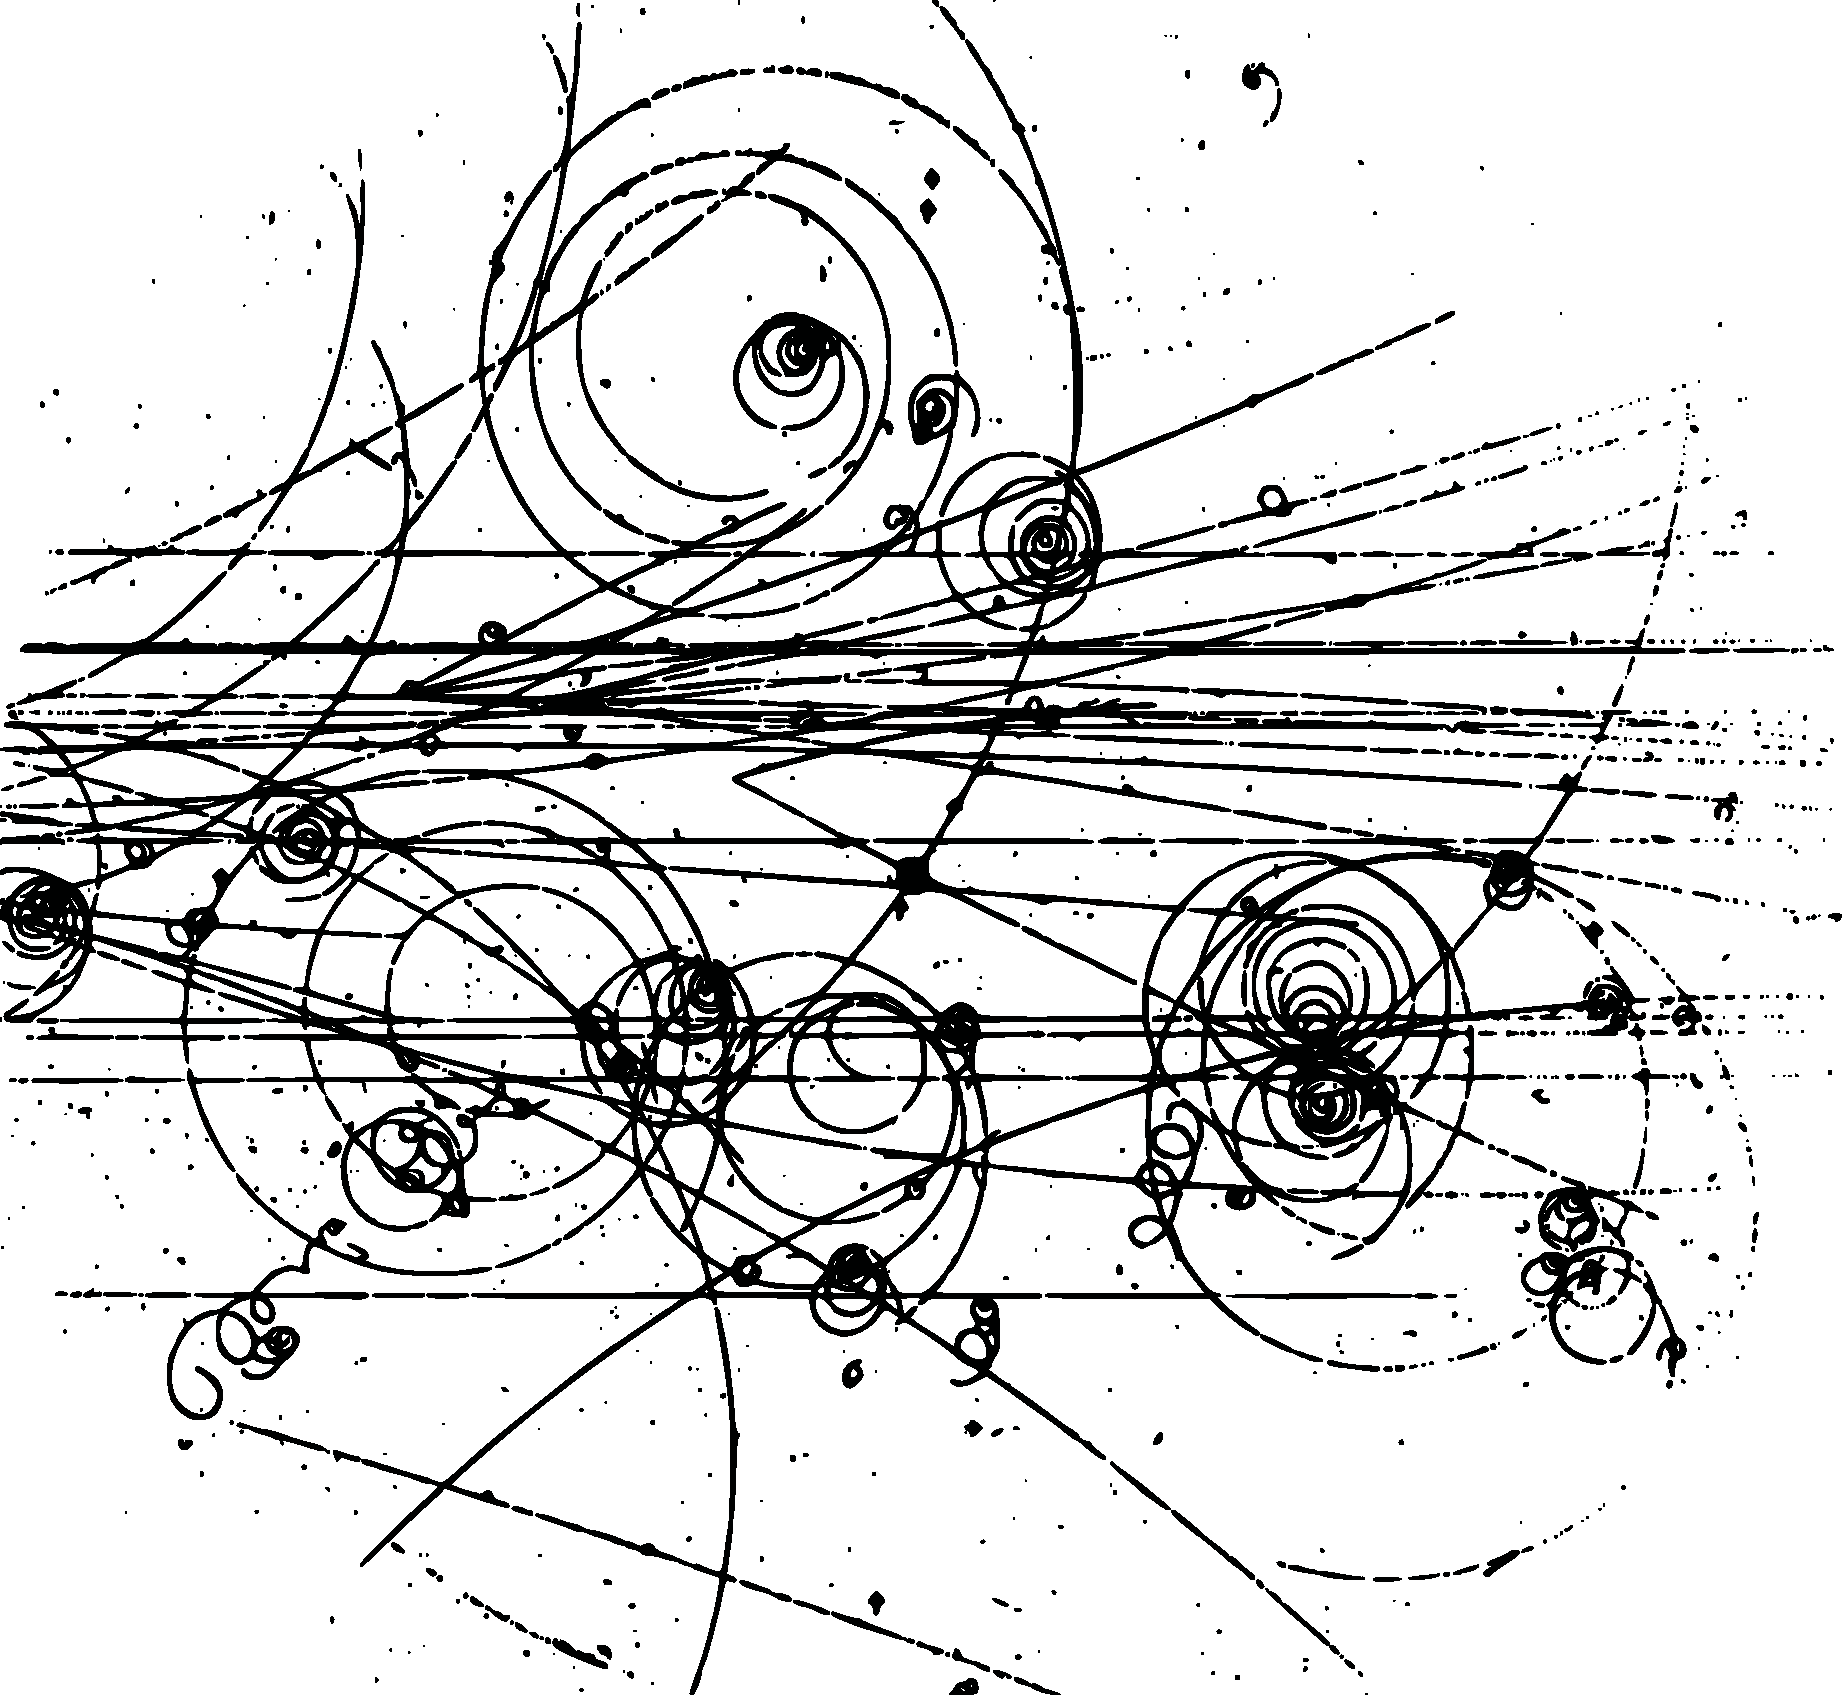
\includegraphics[width=0.6\linewidth]{fig/bc_1}};
%\end{tikzpicture}

\vspace{10cm}
{\huge DOKTORSKA DISERTACIJA}



\vfill

{\hfill \large Matic Lubej}

\vspace{1cm}
{\large 2018}

\cleardoublepage

\end{center}
\end{otherlanguage}

%%% NASLOVNA STRAN V ANGLESKEM JEZIKU
\pagenumbering{roman}
\pagestyle{empty}
\begin{center}


\includegraphics{fig/logo2}

{\large UNIVERSITY OF LJUBLJANA\\
FACULTY OF MATHEMATICS AND PHYSICS\\
DEPARTMENT OF PHYSICS\\}

\vspace{5cm}

{\Large Matic Lubej\\}

\vspace{10mm}

{\bf \Large Measurement of the $\bm{B^+ \to K^+K^-\ell^+\nu_\ell}$ Decay with the Belle Detector\\}
\vspace{5mm}
{\large Doctoral thesis}\\

\vfill

{\large ADVISER: Assist. Prof. Dr. An\v ze Zupanc\\
%COADVISER: Ime in priimek\\
}

\vspace{2cm}
{\large Ljubljana, 2018}

\end{center}


%%% NASLOVNA STRAN V SLOVENSKEM JEZIKU

\cleardoublepage
\begin{otherlanguage}{slovene}
\begin{center}


\includegraphics{fig/logo2}

{\large UNIVERZA V LJUBLJANI\\
FAKULTETA ZA MATEMATIKO IN FIZIKO\\
ODDELEK ZA FIZIKO\\}

\vspace{5cm}

{\Large Matic Lubej\\}

\vspace{10mm}

{\bf \Large Meritev razpada $\bm{B^+ \to K^+K^-\ell^+\nu_\ell}$ z detektorjem Belle\\}
\vspace{5mm}
{\large Doktorska disertacija}\\

\vfill

{\large MENTOR: doc. dr. An\v ze Zupanc\\
%SOMENTOR$\backslash$-ICA: naziv, Ime in priimek\\
}



\vspace{2cm}

{\large Ljubljana, 2018}

\end{center}


%%% ZAHVALA (NEOBVEZNO)

\cleardoublepage

\pagestyle{plain}
\vfill
\chapter*{Zahvala}
Zahvala
\pagestyle{empty}

%%% IZVLECEK

\cleardoublepage
\chapter*{Izvle"cek}
V Disertaciji predstavljamo meritev razvejitvenega razmerja ne-"carobnega semileptonskega razpada \decayb. Meritev je bila opravljena na vzorcu podatkov, ki ustreza integrirani luminoznosti $710\e{fb^{-1}}$, zbranim z detektorjem Belle na asimetri"cnem trkalniku delcev $e^+e^-$ KEKB v mestu Tsukuba na Japonskem. V delu predstavimo rezultate, ki so bili pridobljeni s konverzijo B2BII. To je prva meritev tega razpada, kjer izmerimo razvejitveno razmerje $\mathcal{B}(B^+ \to K^+ K^- \ell^+ \nu) = (3.04 \pm 0.51 \pm {}^{+0.67}_{-0.66})\E{-5}$. S signifikanco $5.9\sigma$ ta meritev "steje kot prvo odkritje razpada.\\
\vspace{1cm}\\
{{\bf Klju"cne besede}:}
\begin{itemize}
	\item detektor Belle
	\item mezoni $B$
	\item semileptonski razpadi
	\item razvejitveno razmerje
\end{itemize}
\vspace{1cm}
{{\bf PACS}:}
\begin{itemize}
	\item 11.30.Er Konjugacija naboja, parnost, obrat "casa in ostale diskretne simetrije
	\item 13.20.-v Leptonski, semileptonski in radiativni razpadi mezonov
	\item 13.20.He Razpadi mezonov s kvarkom $b$
	\item 14.40.Nd Mezoni s kvarkom $b$ ($|B|>0$) 
\end{itemize}
\end{otherlanguage}

\pagestyle{empty}

%%% ABSTRACT
\cleardoublepage
\pagestyle{plain}
\chapter*{Abstract}
We present the branching fraction measurement of the charmless semileptonic decay \decayb. The measurement has been performed on a data sample corresponding to $710\e{fb^{-1}}$ of integrated luminosity, collected with the Belle detector at the KEKB asymmetric-energy $e^+e^-$ collider in Tsukuba, Japan. We present the results obtained with the B2BII data format converter. This is the first measurement of the decay, where we obtain the branching fraction of $\mathcal{B}(B^+ \to K^+ K^- \ell^+ \nu) = (3.04 \pm 0.51 \pm {}^{+0.67}_{-0.66})\E{-5}$. With the fit significance of $5.9\sigma$, this measurement counts as the first discovery of the decay.\\
\vspace{1cm}\\
{{\bf Keywords}:} 
\begin{itemize}
	\item Belle detector
	\item $B$ mesons
	\item semileptonic decays
	\item branching fraction
	\item inclusive tagging
	\item untagged
	\item rest of event
\end{itemize}
\vspace{1cm}
{{\bf PACS}:}
\begin{itemize}
	\item 11.30.Er Charge conjugation, parity, time reversal, and other discrete symmetries
	\item 13.20.-v Leptonic, semileptonic, and radiative decays of mesons
	\item 13.20.He Decays of bottom mesons 
	\item 14.40.Nd Bottom mesons ($|B|>0$) 
\end{itemize}

\pagestyle{empty}

%%% KAZALO
\tableofcontents
\pagestyle{plain}

\chapter{Introduction}

\pagenumbering{arabic}
Particle physics is an established branch of physics with a rich history in theory and experiments ever since the beginning of the 20th century. So far the experimental and theoretical research have shown us hand in hand that the universe consists of particles and force carriers. Particles of matter, or elementary particles, are divided into two groups, quarks and leptons. The quarks that we know today are called $u$ (up), $d$ (down), $s$ (strange), $c$ (charm), $b$ (bottom) and $t$ (top). Leptons are  further split into two groups; charged leptons $e$ (electron), $\mu$ (muon), $\tau$ (tau lepton) and their corresponding neutrinos $\nu_e$ (electron neutrino), $\nu_\mu$ (muon neutrino), $\nu_\tau$ (tau neutrino). Particles of force are known as gauge bosons and they are $\gamma$ (photon), $g$ (gluon), $W^\pm$ (charged weak bosons) and $Z^0$ (neutral weak boson). Theory also predicted the recently discovered Higgs boson ($H$), which is responsible for the mass of all particles. Some of the particles above also have a mirrored version of themselves, called antiparticles, which exhibit somewhat different properties as their un-mirrored versions.

Combinations of quarks such as $q_1 q_2 q_3$ (hadrons) or $q_1 \bar{q}_2$ (mesons) can make up heavier particles that we see today. Such particles are protons and neutrons, but also heavier particles which can be produced in processes involving very high energies. Such heavy particles are unstable and decay into lighter ones via forces of nature. Together with the elementary particles and force carriers, three out of four of these forces are joined in a theoretical model called the Standard Model (SM), which is shown in Figure \ref{fig:sm}. They are the electromagnetic, weak nuclear and strong nuclear force. Gravity is not included in the current version of the Standard Model due to its complex and weakly interacting nature. Researching such processes in large experiments enables us to study the mechanism of how elementary particles interact. By doing so we are able to learn the secrets of the universe and how it all began.

\begin{figure}[!htb]
\centering
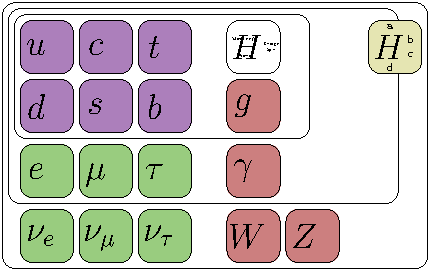
\includegraphics[scale=1.6]{texfig/SM}
\captionsetup{width=.8\linewidth}
\caption{A schematic of the Standard Model.}
\label{fig:sm}
\end{figure}

This analysis revolves around decays of the so-called $B$ mesons, which are particles that consist of a $b$ quark and a light $\bar u$ or $\bar d$ quark (or vice-versa). One of the most surprising features of the universe that can be studied with decays of $B$ mesons is the $CP$ symmetry violation ($\cancel{CP}$). $CP$ symmetry is a combination of the $C$ symmetry (charge conjugation) and the $P$ symmetry (spatial inversion). It states that there is no reason why processes of particles and mirrored processes of antiparticles would be different. Today we know that this does not hold for all cases and we, in fact, find processes which violate this postulate. We also know that $\cancel{CP}$ is very closely related to the weak nuclear force. Here lies our motivation for studying decays of $B$ mesons, since they exhibit a rich spectrum of decays which proceed via the weak nuclear force.

One of the most important properties of the weak nuclear force is that it can change the flavor of particles. Flavor is a quantum number which is conserved for each type of quark, so changing a flavor of a quark means changing the quark itself. Such processes are forbidden for the electromagnetic and the strong nuclear force, but not for the weak one. All of the information regarding quark transitions and transition probabilities can be merged into a form of a complex matrix called the Cabibbo-Kobayashi-Maskawa (CKM) matrix \cite{cabibbo1963unitary,kobayashi1973cp}
\begin{equation}
V_{CKM} = \begin{bmatrix}
    V_{ud} & V_{us} & V_{ub}\\
    V_{cd} & V_{cs} & V_{cb}\\
    V_{td} & V_{ts} & V_{tb}
\end{bmatrix}.
\end{equation}

The CKM matrix is a unitary matrix and has only four free parameters which are not described by theory. Its unitarity provides us with several mathematical identities, out of which the most famous one is
\begin{equation}
V_{ud}V_{ub}^* + V_{cd}V_{cb}^* + V_{td}V_{tb}^* = 0.
\end{equation}

It can be represented by a triangle in the complex plane, called the unitarity triangle, shown in Figure~\ref{ut}. The sides and the angles of the unitarity triangle are closely connected to the free parameters of the CKM matrix. It is important to mention that all experimental measurements depend only on these four parameters, so it is possible to determine them by measuring the angles and sides of the unitarity triangle. This way the unitarity triangle offers us a unique way to test the consistency of the SM. The ultimate goal is to then join all such measurements and overconstrain the unitarity triangle to check if all the sides meet. By improving such measurements one can check whether the SM is consistent, or if there are some contributing physics processes that we do not yet understand. Such processes are commonly referred to as "new physics" (NP). The measurements of the sides and angles of the triangle are done by using different decays of which a large portion are $B$ meson decays. Here lies another motivation for using $B$ mesons in the analysis.

\begin{figure}[!htb]
\centering
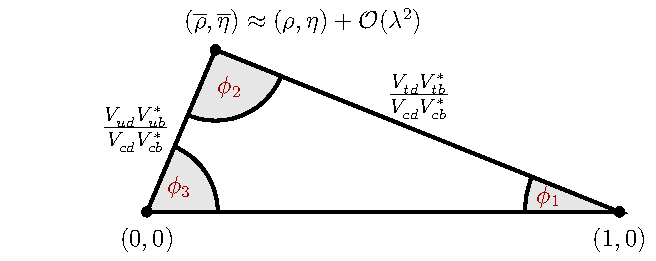
\includegraphics[scale=1]{texfig/UT_Triangle}
\caption{The unitarity triangle with $\lambda,~\eta,~\rho$ and $A$ (not shown) as free parameters of the CKM matrix.}
\label{ut}
\end{figure}

In this analysis, we focus on the $V_{ub}$ CKM matrix element, which corresponds to $b \to u$ quark transitions. It has the smallest absolute value of all the CKM matrix elements and the largest error, so it offers the most room for improvement. Such quark transitions are present in charmless semi-leptonic $B$ meson decays of the form
\begin{equation}
B^+ \to X_u^0 \ell^+ \nu_\ell,
\end{equation}

where $X_u^0$ represents a charmless hadron with a $u$ quark and $\ell$ is one of the charged leptons $e,~\mu$ or $\tau$. Measuring the decay rate of the $B$ meson in such decays paves the way for the CKM matrix element determination. Decay rates are directly connected to the $V_{ub}$ element as
\begin{equation}
\mathrm{d} \Gamma \propto G_F^2 \vert V_{ub} \vert ^2 \vert L^\mu \langle X_u \vert \bar u \gamma_u \frac{1}{2} (1-\gamma_5) b \vert B \rangle \vert ^2,
\end{equation}

where $\Gamma$ is the decay width, $G_F$ is the Fermi coupling constant, $L^\mu$ is the leptonic current and the expression in the Dirac brackets is the hadronic current. The factor $\vert V_{ub} \vert ^2$ represents the probability for the $b \to u$ quark transition. Measurement of the $V_{ub}$ CKM matrix element can be performed in two possible ways. With the exclusive or the inclusive method, which are described below. Both methods require different experimental and theoretical techniques, so they provide largely independent determinations of $\vert V_{ub} \vert$. Currently, both methods also have comparable accuracies. 

In the exclusive method, one studies the decays of $B$ mesons to a specific charmless hadronic final state, such as $B \to \pi \ell \nu$. Clean determination of the $V_{ub}$ is possible due to precise experimental measurements along with reliable theoretical calculations. However, theoretical calculations are more challenging for decays to a specific final state, since hadronization of quarks has to be taken into account. There are also two main experimental challenges in this method. One has to reduce the abundant background from $B \to X_c \ell \nu$ processes since the $b \to c$ quark transition is much more common. The second experimental challenge is to separate the $B$ meson decay with the specific charmless hadronic final state from other $B \to X_u \ell \nu$ decays since it roughly populates the same regions of the phase-space as the signal decay.

In the inclusive method, one studies the decays of $B$ mesons to any charmless hadronic final state $B \to X_u \ell \nu$. In this case, the total decay rate for $b \to u \ell \nu$ can be calculated accurately since hadronization does not have to be taken into account. The greater challenge with this method is again the experimental measurement of the total decay rate due to the $B \to X_c \ell \nu$ background. Experimental sensitivity to $V_{ub}$ is highest where $B \to X_c \ell \nu$ decays are less dominant. Theory and experiment have to compromise and limit the $V_{ub}$ determination to a region where the signal-to-background ratio is good. Theory takes this into account by reliably calculating the partial decay rate $\Delta \Gamma$, which is more challenging than the total decay rate. One possible and often used approach to reduce $b \to c$ background is to reject all events with $K$ particles, or kaons, present in the final particle selection. The procedure is called a $K$-veto. Kaons consist of an $s$ quark, which is mainly produced in $c \to s$ transitions. This means that if a kaon is found in the event, it is very likely that it originates from a particle with a $c$ quark, indicating the $b \to c$ process. 

If $V_{ub}$ is determined with both these methods, the values can be compared. It turns out that consistency between these two results is only marginal, where the difference is at a level of $3\sigma$. The current world averages \cite{Amhis:2016xyh} of the exclusive (from $B^0 \to \pi^- \ell^+ \nu$) and inclusive (GGOU collab. \cite{Gambino:2007rp}) are
\begin{align}
&\vert V_{ub} \vert_{\mathrm{excl.}} = \left(3.65 \pm 0.09 \pm 0.11\right)\E{-3},\\
&\vert V_{ub} \vert_{\mathrm{incl.}}^{\mathrm{GGOU}} = \left(4.52 \pm 0.15~{}^{+0.11}_{-0.14}\right)\E{-3},
\end{align}
where the first and the second errors are the experimental and the theoretical error, respectively. We see that inclusive measurements prefer higher values than exclusive ones. This is known as the $V_{ub}$ puzzle. It is necessary to make further research as to why this difference occurs. The reason could be an unknown experimental or theoretical error, or it is even possible that some NP contributions occur. This analysis will focus on a possible reason that could be hidden in the selection mentioned before. By performing a $K$-veto, one discards all events with kaons in the final state in order to suppress $b \to c$ contributions. In this analysis, we focus on the charged \decaya~decay, which is very similar to the $B \to \pi \ell \nu$, except for a production of an $s \bar s$ quark pair, which then combines with final state quarks to form kaons, as shown in Figure~\ref{feynman}. In this case, we have kaons in the final state where the $B$ meson decayed via a $b \to u$ process. Such decays were discarded in previous $V_{ub}$ determinations with the inclusive method, but in principle, they contribute to the result and should be taken into account. The results of this analysis should help us make a step closer to solving the $V_{ub}$ puzzle. 

\begin{figure}[!htb]
\centering
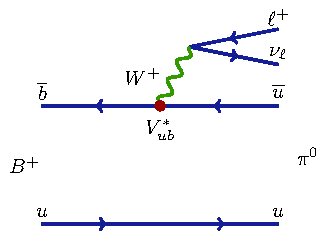
\includegraphics{texfig/B2pilnu}
\hspace{1cm}
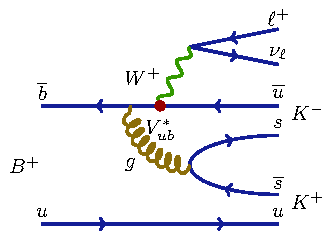
\includegraphics{texfig/B2KKlnu}
\caption{Feynman diagrams for the $B^+ \to \pi^0 \ell^+ \nu_\ell$ decay (left) and the $B^+ \to K^- K^+ \ell^+ \nu_\ell$ decay (right).}
\label{feynman}
\end{figure}

Specifically, we will be focusing on decays of the charged $B$ mesons of the form \decayb, since it includes two charged kaons, as opposed to the case of the neutral $B$ meson decay. The reason for this is a simpler decay chain and a higher reconstruction efficiency. All further occurrences of \decaya~automatically imply decays of the form \decayb~and its charge conjugated counterpart.
\chapter{Data and Monte-Carlo Samples}\label{sec:data-and-monte-carlo-samples}

The Belle detector acquired a dataset of about $L_0 \approx 710\e{fb^{-1}}$ of integrated luminosity in it's lifetime, which corresponds to about $771\E{6}$ $B \bar B$ meson pairs. Additionally, several streams of Monte-Carlo (MC) samples were produced, where each stream of MC corresponds to the same amount of data that was taken with the detector. The main focus of this and other similar analyses is to study a rare signal decay, which means that the amount of such decays in the existing MC is not abundant enough. In such cases, it is a common practice to produce specific samples of signal MC, where the abundance of signal decays is much larger, enabling us to study its properties in greater detail.

The following samples were used in this analysis
\begin{itemize}
	\item data
	\begin{itemize}
		\item Belle on-resonance dataset of about $L_0$ integrated luminosity, measured at $\Upsilon(4S)$ resonance energy,
		\item Belle off-resonance dataset of about $1/10 \times L_0$ integrated luminosity, measured at $60\e{MeV}$ below $\Upsilon(4S)$ resonance energy,
	\end{itemize}
	\item signal MC, corresponding to about $400 \times L_0$,
	\item other MC
	\begin{itemize}
		\item generic on-resonance, $10$ streams of $B\bar B$ (denoted as \texttt{charged} and \texttt{mixed}) and $6$ streams of $q\bar q$ produced at $\Upsilon(4S)$ resonance energy, where each stream corresponds to $L_0$,
		\item generic off-resonance, $6$ streams of $q\bar q$ produced at $60\e{MeV}$ below $\Upsilon(4S)$ resonance energy, where each stream corresponds to $1/10 \times L_0$,
		\item $B\to X_u \ell \nu$ (denoted as \texttt{ulnu}), not included in previous MC samples, equal to an amount of $20 \times L_0$, 
		\item other rare $B$ meson decays (denoted as \texttt{rare}), not included in previous MC samples, equal to an amount of $50 \times L_0$.
	\end{itemize}
\end{itemize}

\section{Signal MC Production}

The signal MC sample of $B^+ \to K^+ K^- \ell \nu_\ell$ and the charge conjugated $B^-$ decays was produced using the \texttt{mcproduzh} package for producing Belle MC. The package accepts a decay file, which describes the decays to be generated. The decay file used for signal MC generation was the same as for the \texttt{ulnu} sample since it includes the decays of interest. An additional skim was applied in order to select only events of interest with at least 2 kaons and a light lepton, all coming from the same particle. This decreases the CPU consumption during the detector simulation and reconstruction.

The relevant processes which contribute to our signal decay are
\begin{itemize}
	\item $B^+ \to a_{00} \ell^+ \nu_\ell$,
	\item $B^+ \to a_{20} \ell^+ \nu_\ell$,
	\item $B^+ \to f_{2} \ell^+ \nu_\ell$,
	\item $B^+ \to f_{0} \ell^+ \nu_\ell$,
	\item $B^+ \to X_{u}^0 \ell^+ \nu_\ell$,
\end{itemize}
where $a_{00}$, $a_{20}$, $f_{2}$ and $f_{0}$ are light unflavored states which include further decays into a $K^+K^-$ pair, and $X_u^0$ represents a generic $u \bar u$ quark pair, which further hadronizes based on the \texttt{PYTHIA} quark hadronization model \cite{sjostrand2006pythia}. Figure \ref{fig:KKsrc} shows the invariant mass of the $KK$ pair from various contributions of the MC generator. The light unflavored states have small contributions with resonant structures, while $KK$ pairs from the $X_u^0$ state are more frequent and follow a wider and smoother distribution.

\begin{figure}[!htb]
	\centering
	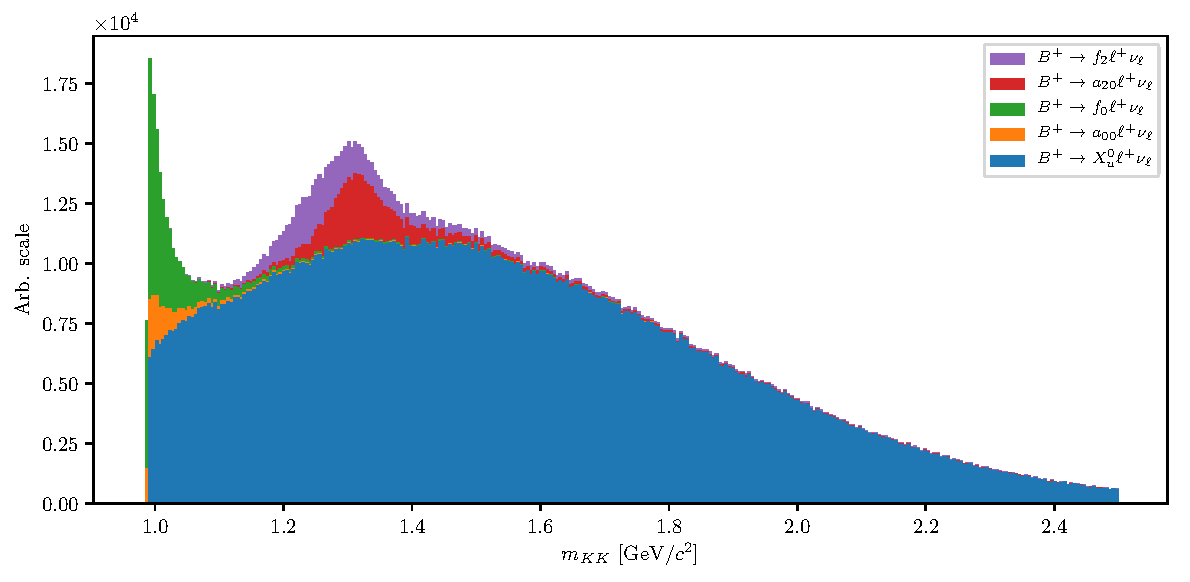
\includegraphics[width=\linewidth]{fig/KKlnu_src}
	\captionsetup{width=.8\linewidth}
	\caption{Invariant mass of the $KK$ pair from various contributions of the MC generator. The light unflavored states have small contributions with resonant structurer, while $KK$ pairs from the $X_u^0$ state are more frequent and follow a wider and smoother distribution.}
	\label{fig:KKsrc}
\end{figure}

The produced signal MC sample contains decays of the form $B \to KK\ell \nu$ as well as $B \to KKX\ell \nu$, where $X$ can be any hadron as long as it satisfies all the selection rules of the decay. It is possible to calculate the MC branching ratios for each channel by making combinations of the particles directly from the generator. Table \ref{tab:KKX} shows some of the most prominent channels, which are similar to our signal decay, as well as their relative fraction. It is clear that our signal decay is the most abundant one, with a relative contribution of about $28.14~\%$, while other channels contribute only up to about $8~\%$ or less. Additionally, our signal decay is the cleanest, while other decays include neutral particles like $\pi^0$, which are harder to reconstruct and suffer from decrease in efficiency due to reconstruction effects.
\begin{table}[!htb]
	\centering
	\begin{tabular}{|l|c|}
		\hline
		Channel & Ratio $[\%]$ \\
		\hline 
		$K^+ K^-$ & 28.14 \\
		\hline
		$K^+ K^- \pi^0$ & 8.94 \\
		\hline
		$K^+ \bar{K}{}^0 \pi^-$ & 8.71 \\
		\hline
		$K^0 K^- \pi^+$ & 8.70 \\
		\hline
		$K^+ K^- \pi^+ \pi^-$ & 4.15 \\
		\hline
		$K^0 \bar K {}^0$ & 3.32 \\
		\hline
		$K^0 \bar K {}^0 \pi^0$ & 3.26 \\
		\hline
		$K^+ K^- \rho^0$ & 1.93 \\
		\hline
		$K^+ \bar{K}{}^0 \rho^-$ & 1.84 \\
		\hline
		$K^0 K^- \rho^+$ & 1.83 \\
		\hline
	\end{tabular}
	\begin{tabular}{|l|c|}
		\hline
		Channel & Ratio \\
		\hline 
		$K^+ K^- \pi^0 \pi^0$ & 0.86 \\
		\hline
		$K^+ K^- \pi^+ \rho^-$ & 0.69 \\
		\hline
		$K^+ K^- \rho^+ \pi^-$ & 0.68 \\
		\hline
		$K^0 \bar K {}^0 \rho^0$ & 0.00 \\
		\hline
		\hline
		$K \bar K$ pair with $\eta$ & 7.08 \\
		\hline
		$K \bar K$ pair with $\omega$ & 5.33 \\
		\hline
		Other & 14.53 \\
		\hline
	\end{tabular}
	\caption{Relative branching ratios of $B \to KKX\ell \nu$ decays by channel.}
	\label{tab:KKX}
\end{table}

We generate about $1.3\E{9}$ events of the form $B\to X_u \ell \nu$, which corresponds to an integrated luminosity of about $L = 400\times L_0$, where this value was obtained by normalizing the signal MC to the amount of signal in the $B\to X_u \ell \nu$ MC sample. This amounts to a total of about $9.37\E{6}$ generated signal events, and to a branching ratio
\begin{equation}
\mathcal{B}\left(B^+ \to K^+ K^- \ell^+ \nu_\ell\right)_{MC} = 1.53\E{-5},
\end{equation}
where $\ell$ is $e$ or $\mu$. During analysis, the abundant signal MC sample is scaled down to correspond to the amount of data taken with the Belle detector.

\section{Control Decay}\label{sec:control-decay}

In this analysis, we are also able to define another $B$ meson decay which occupies almost the same phase space as our signal decay. This process can be used for the monitoring of our analysis steps, which are applied to both measured and simulated data. Any kind of difference between the two might indicate our procedure to be fine-tuned to simulated data, or some other similar problem. 

We define a control decay of the form $$B^+ \to \bar D {}^0 \ell^+ \nu, \quad D^0 \to K^+ K^-,$$ which is much more abundant and, most importantly, easy to suppress since it only populates a very narrow region in the kaon invariant mass spectrum. Due to no extra particles in the $D^0$ decay, the kaon invariant mass is equal to $m_{KK} \approx m_{D^0}$ up to very good precision. By excluding this narrow region we discard the majority of the control candidates while discarding only a small amount of the signal candidates. A more quantitative description of suppressing control and other background candidates is written in chapter \ref{sec:background-suppression}.
\chapter{Experimental Setup}
The data used in this analysis were produced in $e^+e^-$ collisions at the KEKB accelerator and collected with the Belle detector. The experiment was hosted at the High Energy Accelerator Research Organization (KEK) in Tsukuba, Japan. The experiment ran
from years 1999 to 2010, collecting data at and near the energy of the $\Upsilon(4S)$ resonance. This chapter briefly describes the accelerator and the detector, based on detailed reports from \cite{doi:10.1093/ptep/pts102} and \cite{ABASHIAN2002117}, respectively.


\section{KEKB Accelerator}
KEKB is an asymmetric $e^+e^-$ collider, composed roughly of an electron source and a positron target, a linear accelerator (Linac) and two separate main rings with a circumference of about $3\e{km}$ as shown in Figure \ref{fig:kekb}. Electrons are first produced by a thermal electron gun and accelerated in the Linac to an energy of about $8\e{GeV}$. Part of the electrons collide with a tungsten target to produce positrons, which are accelerated in the Linac to an energy of about $3.5\e{GeV}$. Electron and positron beams are injected into the high- (HER) and low energy ring (LER) where they collide as bunches of particles at a single interaction point (IP) at an angle of about $22\e{mrad}$. The combined center-of-mass (CM) energy of the collision corresponds to the mass of the $\Upsilon(4S)$ resonance
\begin{equation}
E_{CM} = \sqrt{2E_{e^+}E_{e^-}} = m_{\Upsilon(4S)}c^2 \approx 10.58\e{GeV}.
\end{equation}

\begin{figure}[!htb]
	\centering
	\captionsetup{width=0.8\linewidth}
	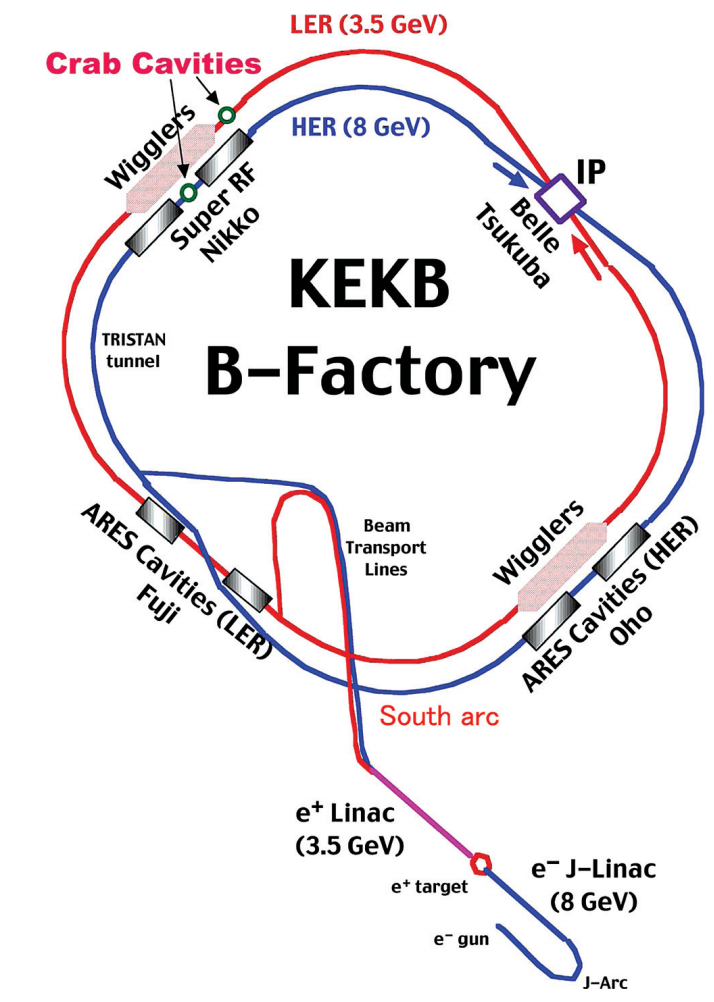
\includegraphics[width=0.5\linewidth]{fig/setup/KEKB}
	\caption{Schematic layout of the KEKB accelerator. The HER and the LER are the $e^-$ and the $e^+$ beams, respectively. Four experimental halls, FUJI, NIKKO, OHO and TSUKUBA are shown.}
	\label{fig:kekb}
\end{figure}

The $\Upsilon(4S)$ state is produced only in a fraction of all collisions, but when it is produced, it predominantly decays to a pair of charged or neutral $B$ mesons. This setup was chosen in accordance with the main goal of the experiment, which was to study CP
violation in the $B$ meson system. In other cases, the processes include $e^+e^-$ scattering, also known as Bhabha scattering, two-photon events, muon or tau lepton pair production, and production of $q \bar q$, where $q=u,\,d,\,s$ or $c$. Table \ref{tab:xsec} shows the cross-sections for all mentioned interactions in collisions of $e^+e^-$.
In addition to the nominal CM energy, the experiment collected data also at energies
corresponding to other $\Upsilon(nS)$ resonances, where $n = 1,\,2,\,3,\,5$, and also at energies below the resonances.

\begin{table}[!htb]
	\centering
	\begin{tabular}{|c|c|}
		\hline
		Interaction & Cross-section $[\mathrm{nb}]$ \\ 
		\hline
		$\Upsilon(4S) \to B \bar B$ & $1.2$ \\
		$q \bar q,~q \in [u,d,s,c]$ & $2.8$ \\
		$\mu^+\mu^-,~\tau^+\tau^-$ & $1.6$ \\
		Bhabha scattering (within detector acceptance)& $44$ \\
		Other QED processes (within detector acceptance)& $\sim 17$ \\
		\hline
		Total & $\sim 67$ \\
		\hline
	\end{tabular}
	\caption{Cross-sections with $L=10^{34}\e{cm^{-2}s^{-1}}$ for various physics processes at $\Upsilon(4S)$ resonance energy \cite{ABASHIAN2002117}.}
	\label{tab:xsec}
\end{table}

KEKB achieved the world-record for the peak luminosity of $2.11\E{34}\e{cm^{-2}s^{-1}}$, twice as much as the designed prediction, and the total integrated luminosity of $1041\e{fb^{-1}}$. Of the full Belle dataset, about $711\e{fb^{-1}}$ of data were taken at the $\Upsilon(4S)$ energy of $10.58\e{GeV}$, which corresponds to about $771\E{6}$ $B \bar B$ meson pairs.

\section{Belle Detector}
The Belle detector is a magnetic mass spectrometer which covers a large solid angle. It is designed to detect remnants of $e^+e^-$ collisions. The detector is configured around a $1.5\e{T}$ superconducting solenoid and iron structure surrounding the interaction point (IP). The 4-momentum of the decaying $B$ mesons and it's decayed daughter particles are determined via a series of sub-detector systems, which are installed in an onion-like shape. Short-lived particle decay vertices are measured by the silicon vertex detector (SVD) situated outside of a cylindrical beryllium beam pipe. Long-lived charged particle momentum is measured via tracking, which is performed by a wire drift chamber (CDC). Particle identification is provided by energy-loss measurements in CDC, aerogel Cherenkov counters (ACC) and time-of-flight counters (TOF), situated radially outside of CDC. Particles producing electromagnetic showers deposit energy in an array of CsI(Tl) crystals, known as the electromagnetic calorimeter (ECL), which is located inside the solenoid coil. Muons and $K_L$ mesons (KLM) are identified by arrays of resistive plate counters in the iron yoke on the outside of the coil. 

The coordinate system of the Belle detector originates at the IP, with the $z$ axis pointing in the opposite direction of the positron beam, the $x$ axis pointing horizontally out of the ring, and the $y$ axis being perpendicular to the aforementioned axes. Th electron beam crosses the positron beam at an angle of about $22^\circ$. The polar angle $\theta$ covers the region between $17^\circ \leq \theta \leq 150^\circ$, while the cylindrical angle $\varphi$ covers the full $360^\circ$ range, amounting to about $92\%$ coverage of the full solid angle.

%TODO: add detector image


%In our analysis, key features of the Belle detector are as follows.
%•
%Good particle detection efficiency for 4-
%π
%region to collect all the particles in an
%e
%+
%e
%−
%collision.  This is important not only for the good signal reconstruction efficiency,
%but also for background reduction since un-detected particles from various
%B
%decay
%modes are the main source of the background.
%•
%Good reconstruction efficiency for low-momentum particles.  Since decay particles
%from
%D
%∗
%mesons and
%τ
%leptons are produced in a chain of multi-body decays, their
%momenta are about 0.7 GeV
%/c
%on average and lower than 1.5 GeV
%/c
%.
%•
%Good  momentum  resolution  in  the  tracking  devices  and  energy  resolution  in  the
%ECL.
%•
%Good PID performance for charged particles.

%\subsection{Extreme forward calorimeter (EFC)}

\subsection{Silicon Vertex Detector}
SVD is the inner-most part of the Belle detector and serves the purpose of measuring the decay vertices of decaying particles. The precision of the subsystem is about $100\e{\mu m}$, which is important for measuring the difference in $z$-vertex positions of the $B$ mesons in time-dependent CP violation studies. The main parts of the SVD are the double-sided silicon detectors (DSSD). With their thin profile and parallel silicon strips on both sides they provide 2D hit information of charged particle and are perfect for a small-scale device which acts with high precision.

During the data taking period, two configurations of the SVD have been used. The first, SVD1, has three layers of DSSD detectors, positioned at $30$, $45.5$ and $60\e{mm}$ away from the IP. They compose a ladder-like structure, covering the polar angle of $23^\circ < \theta < 140^\circ$. This configuration was used from the beginning of the experiment until 2003 when a dataset of about $1.52\E{8}$ pairs of $B \bar B$ mesons were recorded. Due to problems with radiation hardness, a new configuration was used, SVD2, which was operational until the end of data taking, measuring about $6.20\E{8}$ pairs of $B \bar B$ mesons. The SVD2 has 4 layers of DSSD detectors positioned at $20$, $43.5$, $70$ and $80\e{mm}$ away from the IP and covered the polar angle of $17^\circ < \theta < 150^\circ$. The first layer was moved closer to the IP, which greatly improved the sub-system precision, due to multiple-Coulomb scattering affecting resolution more as the distance from the IP increases. The front and side view of the SVD2 are shown in Figure \ref{fig:SVD_layout}.

\begin{figure}[!htb]
	\centering
	\captionsetup{width=0.8\linewidth}
	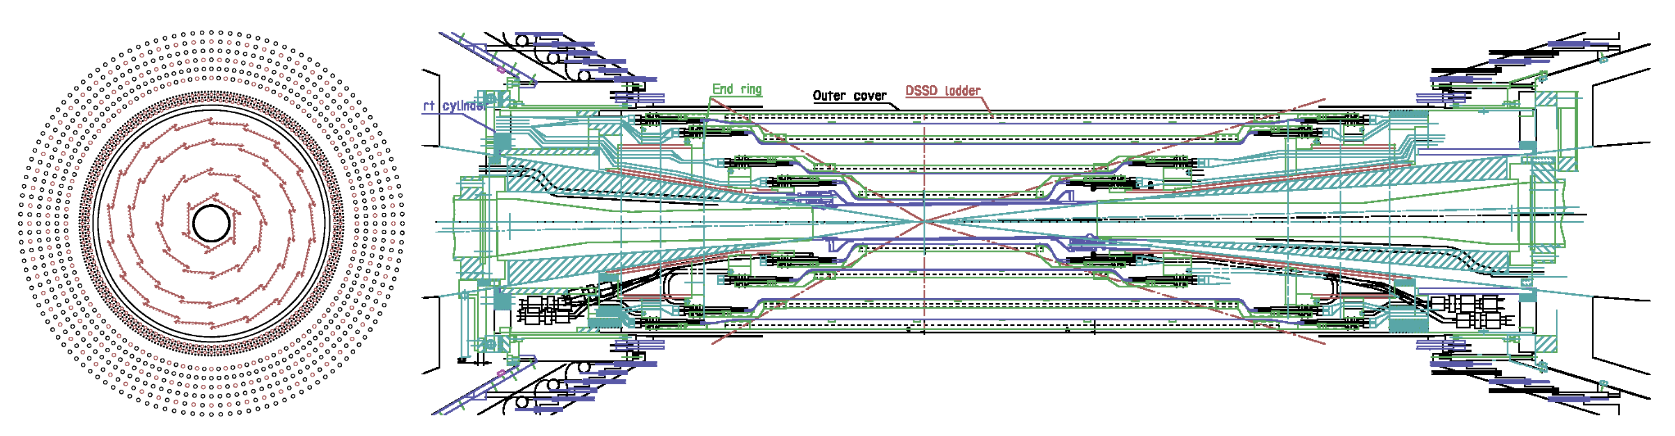
\includegraphics[width=\linewidth]{fig/setup/SVD_layout}
	\caption{Front (left) and side (right) view of the SVD detector with the SVD2 configuration. The front view also shows the inner wires of the
		Drift Chamber \cite{haba2004letter}.}
	\label{fig:SVD_layout}
\end{figure}

The efficiency of the SVD was determined as a fraction of CDC tracks within the SVD acceptance that have associated SVD hits, needed for the $B$ meson reconstruction. The average efficiency is found to be around $98\%$ and is in agreement with simulation. SVD performance is also determined via the impact parameter $z$ and $r\phi$ resolution, which was obtained from cosmic ray data. The momentum and angular dependence of the impact parameters is shown in Figure \ref{fig:SVD_performance} and is well represented by the following parametrization for the SVD2
\begin{align}
\sigma_z = 28\e{\mu m}\oplus \frac{32\e{\mu m}}{\left(p/(1\e{GeV}/c)\right)}\frac{1}{\beta \sin^{5/2}\theta},\\
\sigma_{r\phi} = 22\e{\mu m}\oplus \frac{36\e{\mu m}}{\left(p/(1\e{GeV}/c)\right)}\frac{1}{\beta \sin^{3/2}\theta},
\end{align}
where $p$ is the particle momentum, $\theta$ is the polar angle, and $\beta=v/c$. An advantage of the smaller distance between the IP and the first DSSD layer in SVD2 is clearly seen.

\begin{figure}[!htb]
	\centering
	\captionsetup{width=0.8\linewidth}
	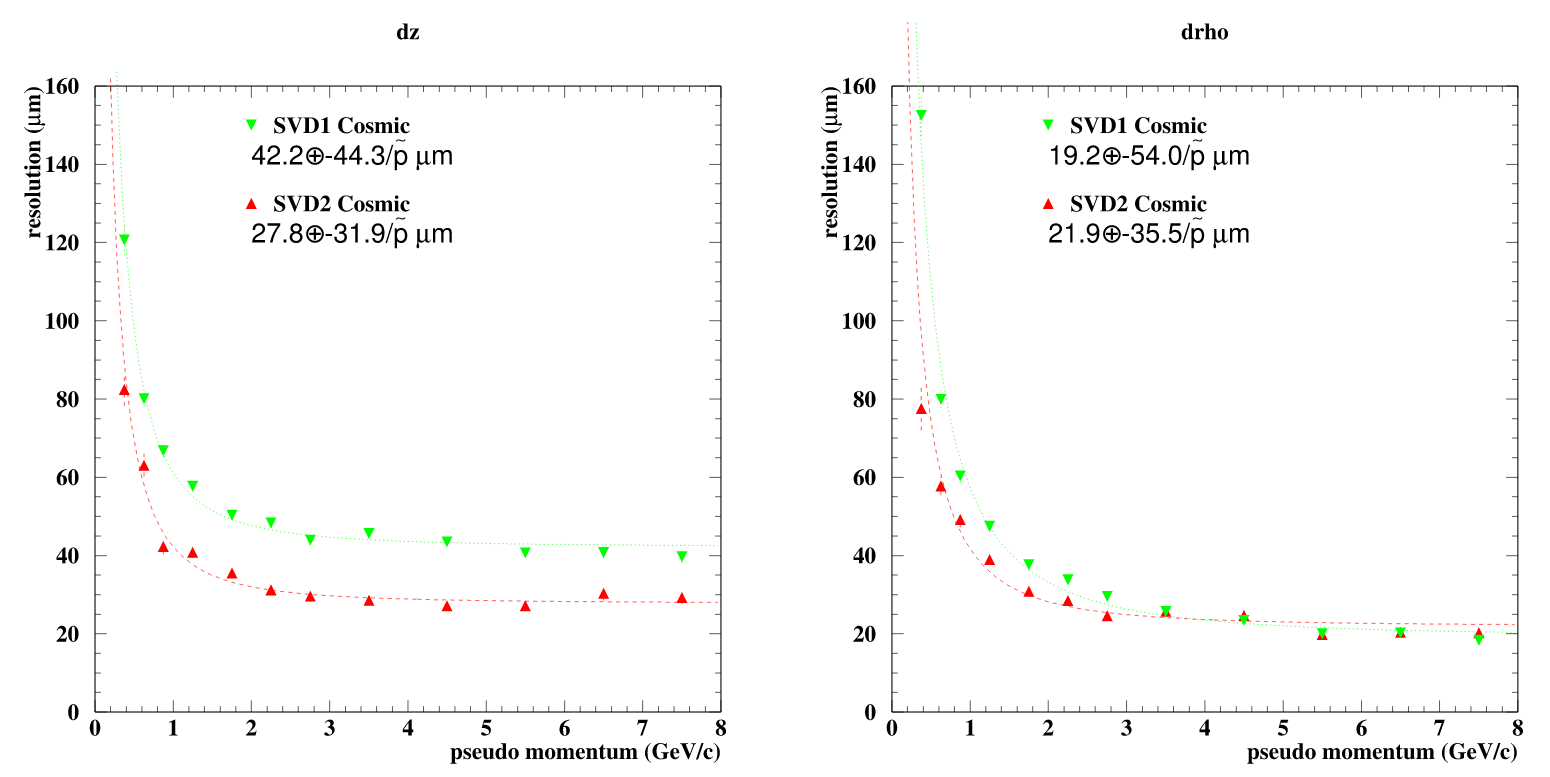
\includegraphics[width=\linewidth]{fig/setup/SVD_performance_1}
	\caption{Impact parameter resolutions of $z$ (left) and $r\phi$ (right) coordinates for the SVD1 and SVD2 configuration of the vertex detector \cite{haba2004letter}.}
	\label{fig:SVD_performance}
\end{figure}


\subsection{Central Drift Chamber}

CDC is a large-volume tracking device located at the central part of the Belle detector and is crucial for measurements of the particle trajectories and momenta, but also serves as a particle identification device (PID). It has a cylindrical structure with a radius of $88\e{cm}$, length of $2.4\e{m}$ and acceptance equal to the one of SVD2. The chamber has a total of $8400$ wires, which are positioned in $50$ layers and describe a nearly square wire configuration. There are two types of wires -- field wires for producing the electrical field, and sense wires for detecting the particles. Odd-numbered wire layers are oriented in the $z$ direction and provide a measurement of the transverse momentum $p_t$, while even-numbered wires are inclined with respect to the $z$ axis by a small angle of $\pm 50\e{mrad}$ to allow for measuring of the polar angle of the track. The wire configuration is shown in Figure \ref{fig:CDC_layout}. The space between the wires is filled with a gas mixture of $1:1$ helium-ethane, a low-$Z$ gas in order to minimize multiple-Coulomb scattering contributions to momentum resolution, since the majority of particles in $B$ events have a momentum lower than $1\e{GeV}/c$. It also has a small cross section of the photoelectric effect, which is important to reduce background electrons induced by the synchrotron radiation from the beam. 

\begin{figure}[!htb]
	\centering
	\captionsetup{width=0.8\linewidth}
	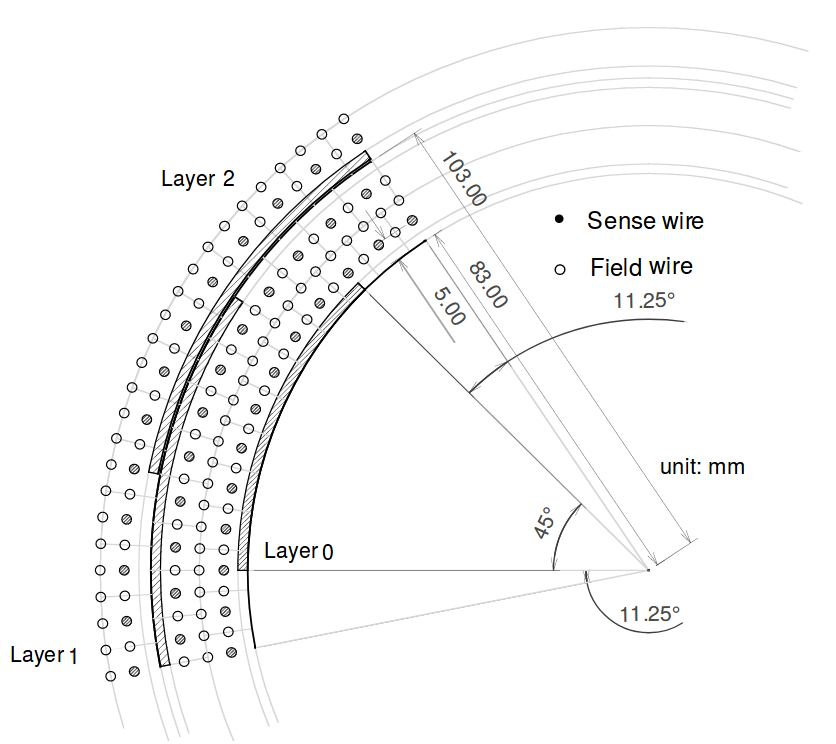
\includegraphics[width=0.6\linewidth]{fig/setup/CDC_layout}
	\caption{Cell structure of CDC \cite{ABASHIAN2002117}.}
	\label{fig:CDC_layout}
\end{figure}

Charged particles which pass the CDC wire frame cause gas ionization. The produced electrons drift toward the sense wires with great acceleration due to the strong electric field close to the wire. The accelerated electrons collide with gas molecules and produce secondary, tertiary etc. ionizations, which result in an electron avalanche, a process which increases the signal by many orders of magnitude. The primary electrons also have a specific drift velocity, which allows us to relate the measured pulse height and drift time to the energy deposit of the particle as well as the distance from the sense wire. This information is important for calculating the energy loss $\mathrm{d}E/\mathrm{d}x$. $\mathrm{d}E/\mathrm{d}x$ as a function of momentum differs for different particles, as shown in Figure \ref{fig:dEdx}. This allows for identification purposes of, specifically for kaons and pions. In the momentum region less than $0.8\e{GeV}/c$, $\mathrm{d}E/\mathrm{d}x$ enables a separation between kaons and pions up to $3\sigma$. The resolution of the transverse momentum measurement with the CDC is a function of the transverse momentum itself, as well as the particle velocity, and is parametrized as
\begin{equation}
\sigma(p_T)/p_T = \frac{0.201\%~p_T}{1\e{GeV}/c} \oplus \frac{0.290\%}{\beta}.
\end{equation}

\begin{figure}[!htb]
	\centering
	\captionsetup{width=0.8\linewidth}
	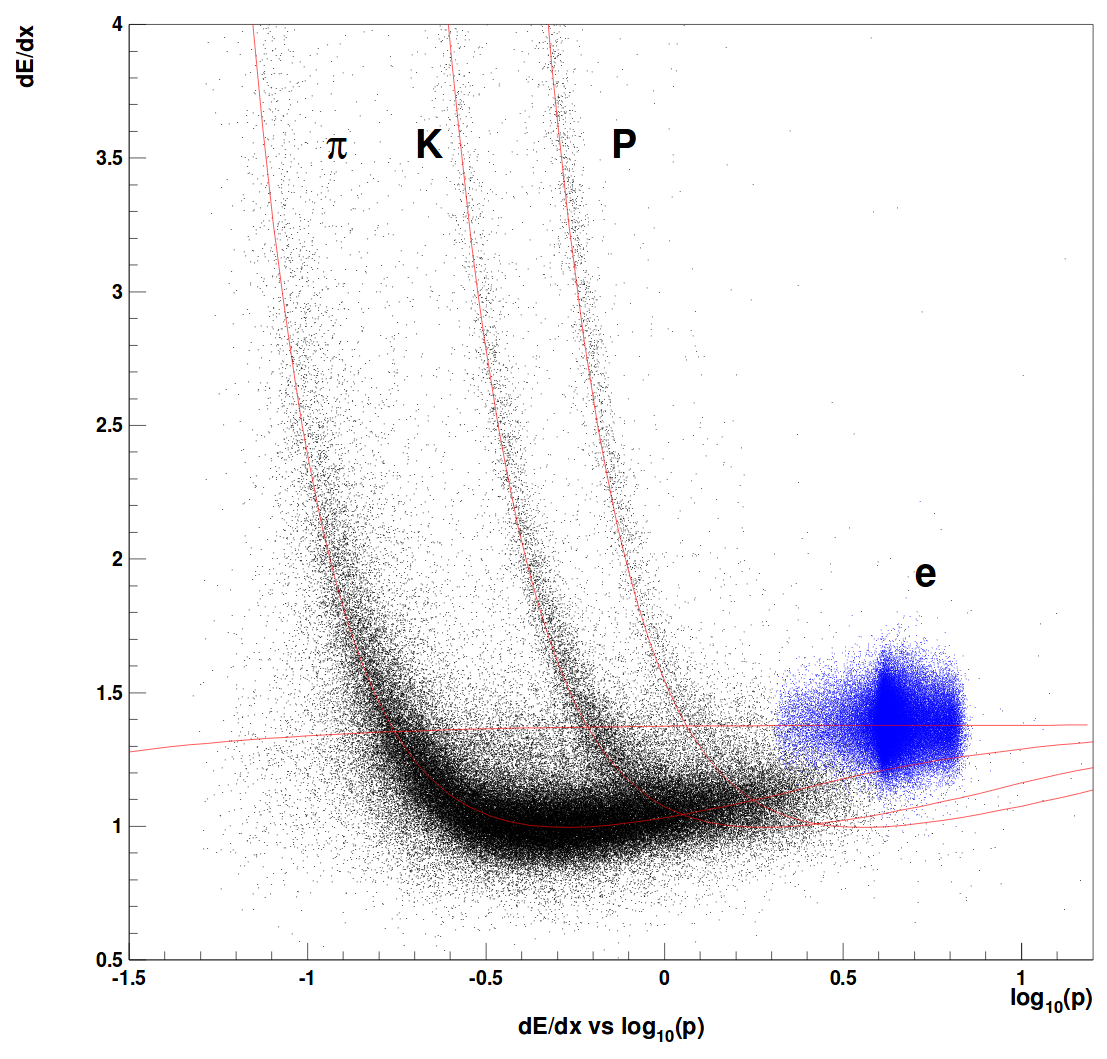
\includegraphics[width=0.6\linewidth]{fig/setup/dEdx}
	\caption{Measured $\mathrm{d}E/\mathrm{d}x$ as a function of particle momentum. The red lines show the expected distribution for different types of particles \cite{ABASHIAN2002117}.}
	\label{fig:dEdx}
\end{figure}

\subsection{Time-of-Flight Counter}

The purpose of the TOF subdetector is particle identification in the momentum region $0.8\e{GeV}/c < p < 1.2\e{GeV}/c$, especially for kaons and pions. There are 64 TOF modules in the barrel region, covering the polar angle of $33^\circ < \theta < 121^\circ$. One TOF module consists of two long polyvinyl toluene-based plastic scintillator bars, 4 fine-mesh photo-multiplier tubes (PMT) at the 4 ends of the bars, and a trigger scintillation counter, where the latter provides additional trigger information. TOF measures the time interval between the $e^+e^-$ collision and the passage of the particle through it. The mass of a particle can be inferred via the relation
\begin{equation}
m^2 = \left( \frac{1}{\beta^2}-1\right)p^2 = \left( \frac{T^2c^2}{L^2}-1\right)p^2,
\end{equation}
where $T$ is the measured time interval, $L$ is the charged particle trajectory length from the IP to TOF and $p$ is the charged particle momentum, determined by SVD and CDC. The resulting mass distribution for charged tracks measured by TOF in hadron events is shown in Figure \ref{fig:TOF_mass}, where clear peaks corresponding to pions, kaons and protons can be seen. To achieve the good discrimination between kaons and pions, a time-of-flight resolution of less than $100\e{ps}$ is needed for particles with momentum below about $1.2\e{GeV}/c$, which encompasses $90\%$ of the particles produced in $\Upsilon(4S)$ decays. The identification power can also be determined in the form of $\pi^\pm/K^\pm$ separation significance as a function of particle momentum, shown in Figure \ref{fig:TOF_separation}. A clear separation of about $2\sigma$ is achieved for particle momenta up to $1.25\e{GeV}/c$.

\begin{figure}[!htb]
	\centering
	\captionsetup{width=0.8\linewidth}
	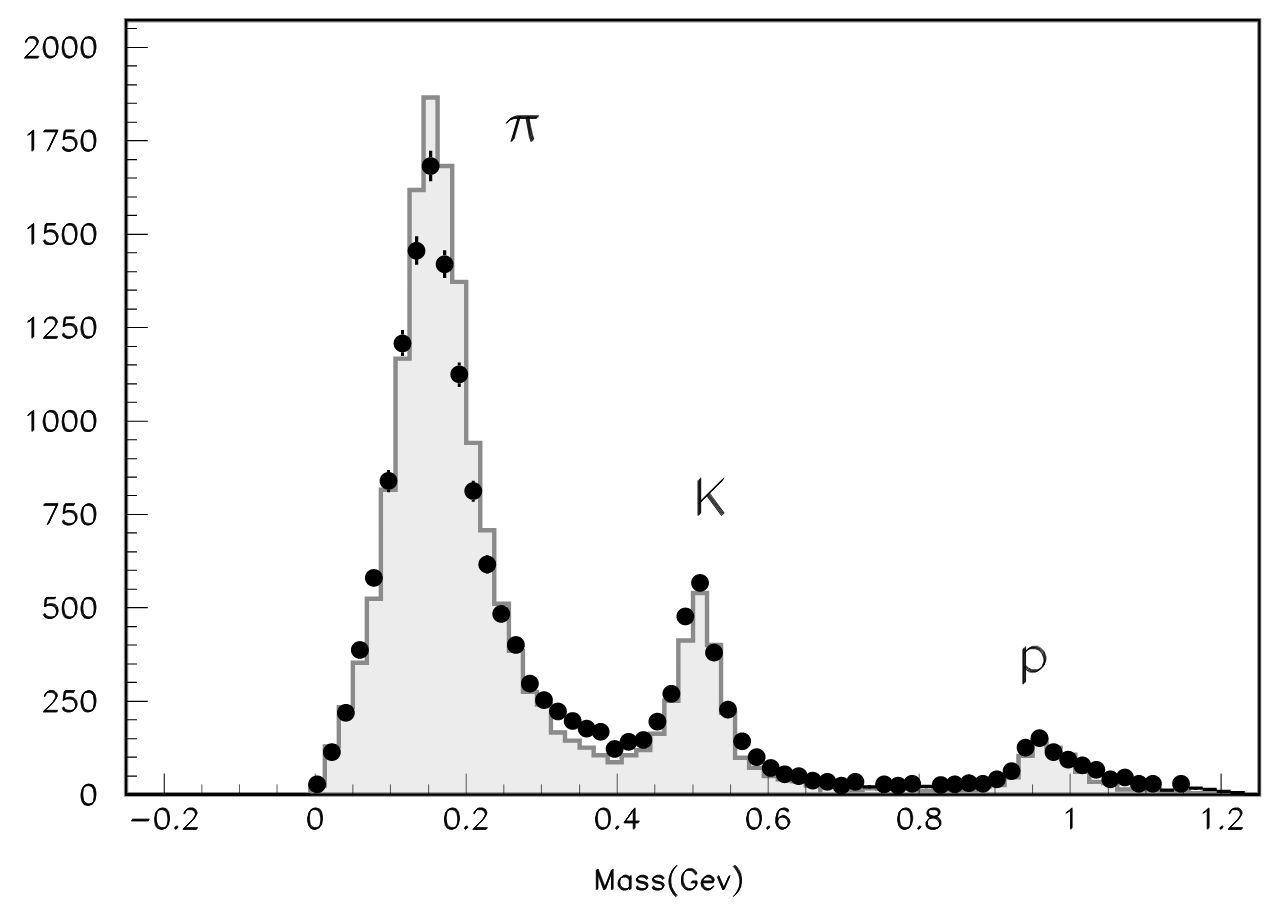
\includegraphics[width=0.6\linewidth]{fig/setup/TOF_mass}
	\caption{Mass distribution from TOF measurements for particle momenta below $1.2\e{GeV}/c$ \cite{ABASHIAN2002117}.}
	\label{fig:TOF_mass}
\end{figure}

\begin{figure}[!htb]
	\centering
	\captionsetup{width=0.8\linewidth}
	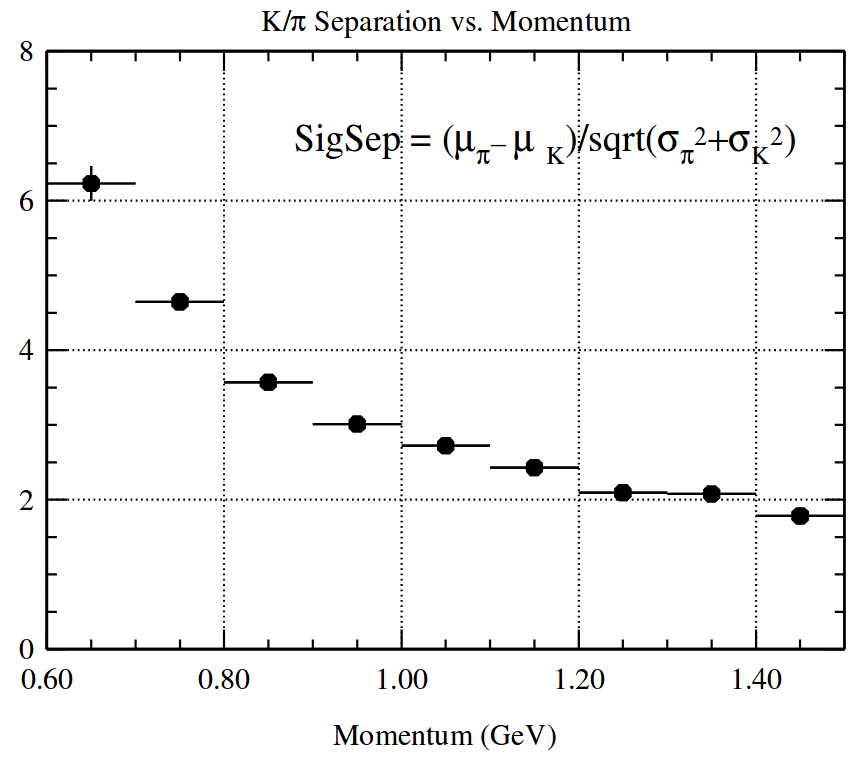
\includegraphics[width=0.6\linewidth]{fig/setup/TOF_separation}
	\caption{$\pi^\pm/K^\pm$ separation by TOF \cite{ABASHIAN2002117}.}
	\label{fig:TOF_separation}
\end{figure}


\subsection{Aerogel Cherenkov Counter}
TOF is not capable of performing good PID above $1.2\e{GeV}/c$ momentum since $\beta$ is almost equal to 1. For higher momenta in the region $1.0\e{GeV}/c < 4.0\e{GeV}/c$, the ACC is introduced. It is a threshold-type Cherenkov counter which utilizes the fact that particles emit Cherenkov light if the particle speed is greater than the speed of light in the passing medium. ACC is introduced in the barrel region with 960 separate modules, covering a polar angle of $34^\circ < \theta < 127^\circ$ and 228 modules in the forward end-cap region, with the polar angle coverage of $17^\circ < \theta < 34^\circ$. Each ACC module consists of an aluminum encased block of silica aerogel and one or two fine-mesh PMTs encased on each block to detect Cherenkov light pulses. Due to the polar angle dependence of the particle momentum, 6 different refractive indices are chosen for the aerogel material, ranging from $1.010$ up to $1.030$ and are controlled within $3\%$ precision. The layout of the ACC is shown in Figure \ref{fig:ACC_layout}.
\begin{figure}[!htb]
	\centering
	\captionsetup{width=0.8\linewidth}
	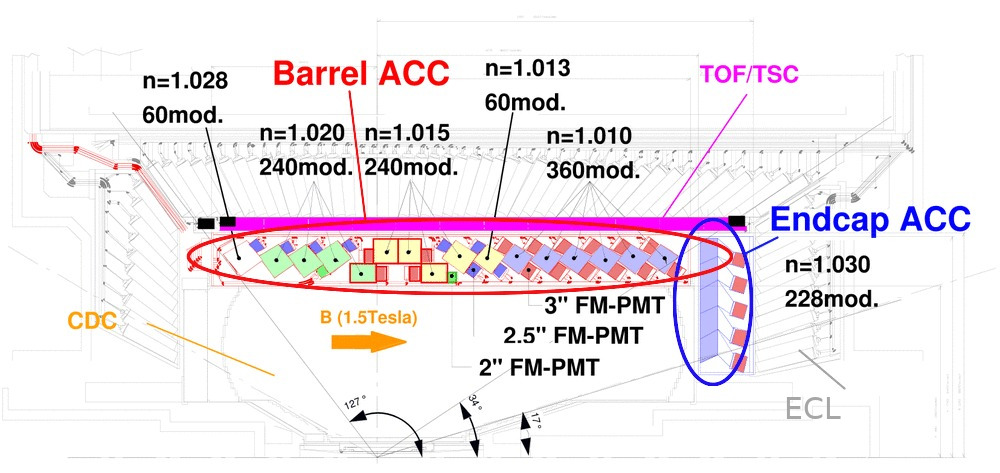
\includegraphics[width=\linewidth]{fig/setup/ACC_layout}
	\caption{Cross-sectional view of the CDC (inner most), ACC and TOF (outer most) detectors \cite{ABASHIAN2002117}.}
	\label{fig:ACC_layout}
\end{figure}
The threshold velocity $\beta$ of a given particle for Cherenkov radiation is
\begin{equation}
\beta \leq \frac{1}{n},
\end{equation}
where $n$ is the refractive index of the medium. The refractive indices in the ACC are such that, due to different masses, pions will emit Cherenkov light and kaons will not, due to different masses of the particles. Using the PID of ACC, along with other sub-system PID info, the electron identification efficiency in the momentum range above $1\e{GeV}/c$ is equal to or above $90\%$ while the pion fake rate, the probability of wrongly identifying pions as electrons, to be around $0.2$ - $0.3\%$. Similarly for kaons, kaon ID efficiency is equal to $80\%$ for most of the momentum region up to $4\e{GeV}/c$, while pion fake rate remains below $10\%$. Figure \ref{fig:ACC_eff} shows the electron and kaon efficiencies and the corresponding pion fake rates as a function of particle momenta.

\begin{figure}[!htb]
	\centering
	\captionsetup{width=0.8\linewidth}
	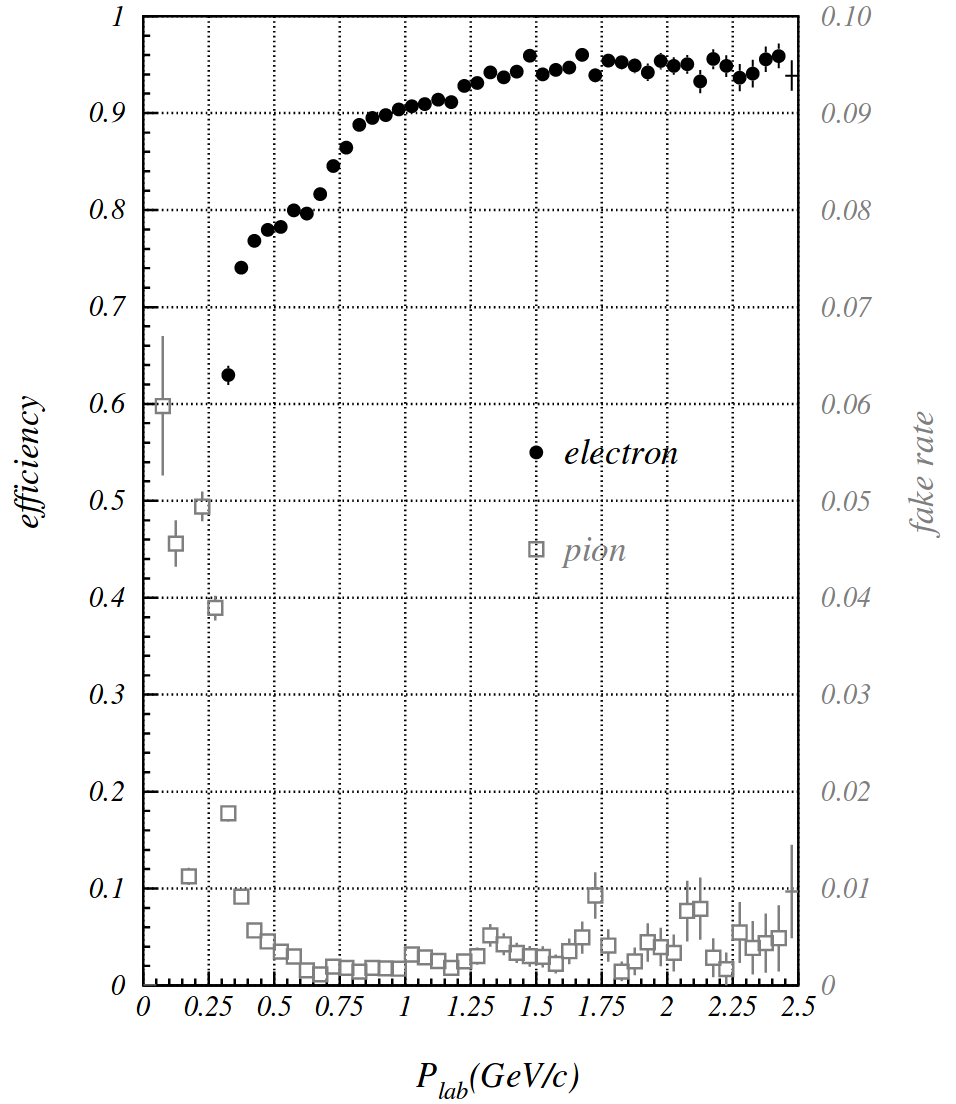
\includegraphics[width=0.48\linewidth]{fig/setup/ACC_eff1}
	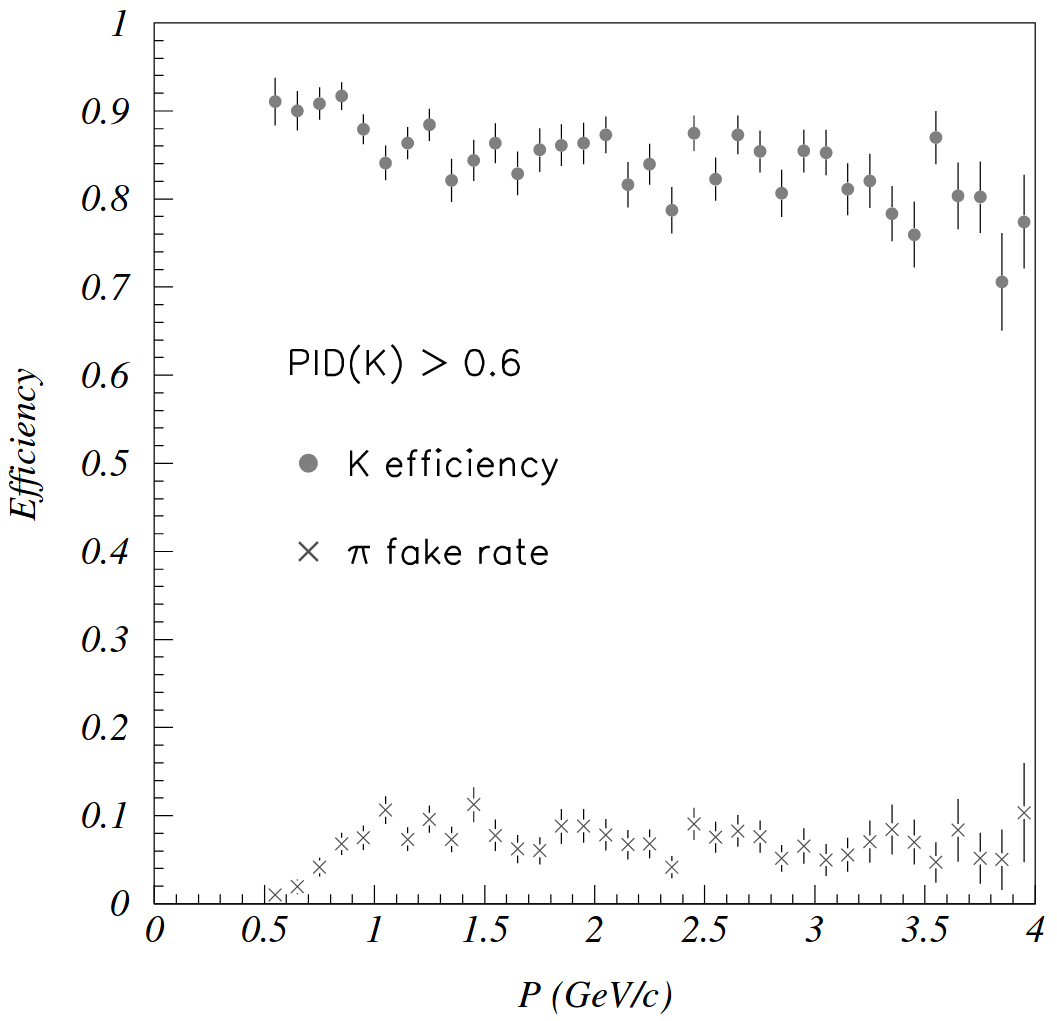
\includegraphics[width=0.48\linewidth,trim = 0cm -4cm 0cm 0cm]{fig/setup/ACC_eff2}
	\caption{Electron identification efficiency and fake rate for charged pions (left) and similarly for kaons (right). Note the different scales for the electron efficiency and fake rate in the former case \cite{ABASHIAN2002117}.}
	\label{fig:ACC_eff}
\end{figure}


\subsection{Electromagnetic Calorimeter}
Measurement of position and energy deposit of particles is performed in the ECL, especially for electrons and photons, where the latter are not measured by any of the subsystems described so far. It also provides complimentary particle identifications for electrons versus pions. The calorimeter consists of a highly segmented array of thallium-doped cesium iodide (CsI(Tl)) in the form of tower-shaped crystals, each pointing towards the IP. Each crystal is about $30\e{cm}$ long with a width from $44.5\e{mm}$ to $65\e{mm}$ in the barrel, and from $44.5\e{mm}$ to $82\e{mm}$ in the end-caps. Out of a total of 8736 crystals with a total mass of about $43\e{tons}$, 6624 of them are positioned in the barrel region and 1152 (960) in the forward (backward) end-caps. The inner radius of the barrel section is about $1.25\e{m}$, while the end-caps are positioned at $-1.0\e{m}$ and $2.0\e{m}$ from the IP in direction of the $z$ axis. The polar angle coverage of the barrel region is $32.2^\circ < \theta < 128.7^\circ$, and for the end-caps $12.4^\circ < \theta < 31.4^\circ$ and $130.7^\circ < \theta < 155.1^\circ$. Figure \ref{fig:ECL_layout} shows the layout of the barrel and end-caps ECL. 
\begin{figure}[!htb]
	\centering
	\captionsetup{width=0.8\linewidth}
	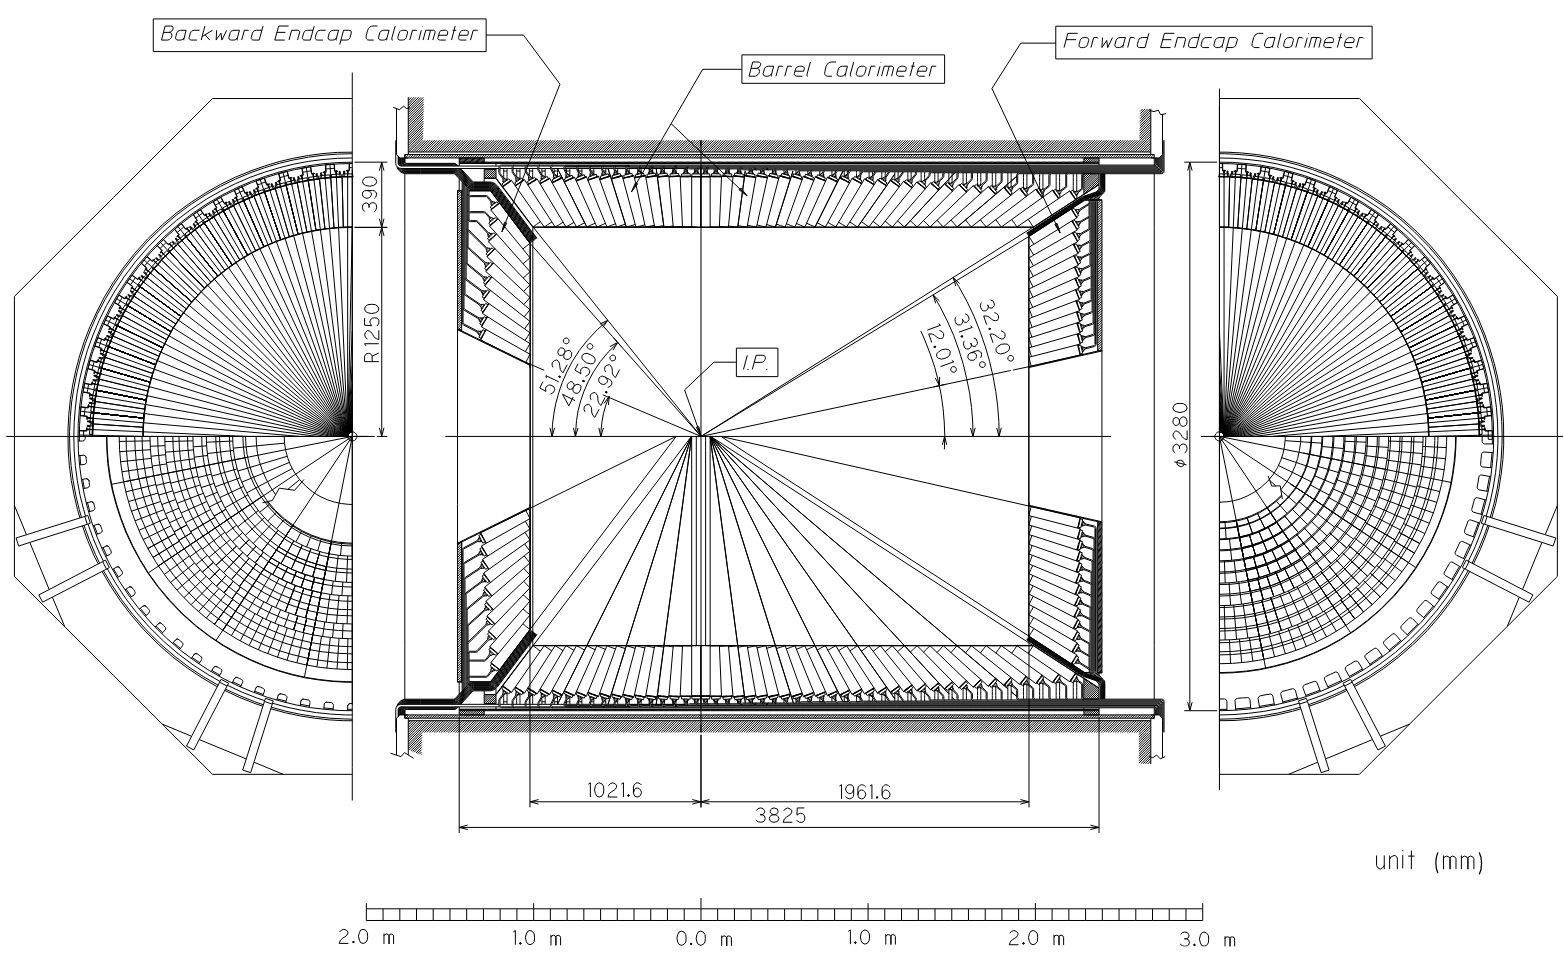
\includegraphics[width=\linewidth]{fig/setup/ECL_layout}
	\caption{Overall configuration of the ECL \cite{ABASHIAN2002117}.}
	\label{fig:ECL_layout}
\end{figure}
When an electron or a photon hits a crystal, it produces an electromagnetic shower, a result of the bremsstrahlung and pair-production effects. Heavier charged particles do not interact in the same way and deposit only a small amount of energy by ionization effects. The information from the ECL, compared with momentum measurements provided by the CDC, enables the identification of electrons. The distribution of the deposited energy for different particles is shown in Figure \ref{fig:ECL_deposit}. The probability of misidentifying an electron as a pion is approximately $5\%$ for momenta less than $1\e{GeV}/c$, and less than $1\%$ for momenta above $2\e{GeV}/c$.

\begin{figure}[!htb]
	\centering
	\captionsetup{width=0.8\linewidth}
	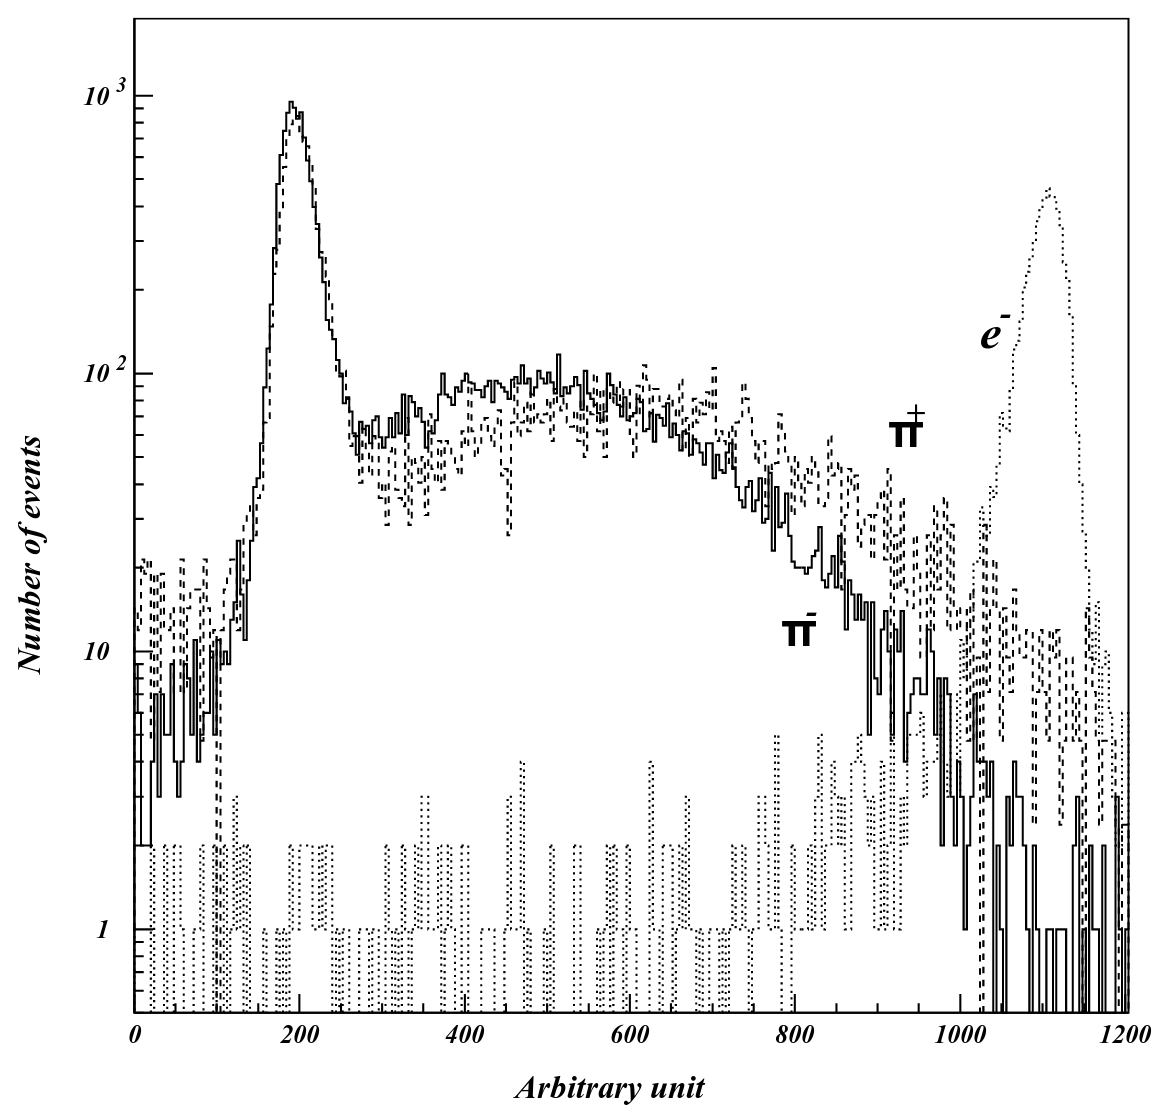
\includegraphics[width=0.6\linewidth]{fig/setup/ECL_deposit}
	\caption{Distribution of the energy deposit by electrons and charged pions at $1\e{GeV}/c$ momentum \cite{ABASHIAN2002117}.}
	\label{fig:ECL_deposit}
\end{figure}

For ECL calibration, $e^+e^- \to e^+e^-$ and $e^+e^- \to \gamma\gamma$ events were used. The average energy resolution was achieved to be $1.7\%$ for the barrel ECL, and $1.74\%$ and $2.85\%$ for the forward and backward ECL, respectively, as shown in Figure \ref{fig:ECL_resolution}. These value are in good agreement with Monte Carlo predictions. Worse energy resolution in backward end-cap is due to the lower photon energy, which results in larger effects of passive material in front of the calorimeter \cite{haba2004letter}. The energy resolution as a function of energy can be obtained via the following relation
\begin{equation}
\frac{\sigma_E}{E} = \frac{0.0066\%}{\left(E/1\e{GeV}\right)}\oplus\frac{1.53\%}{\left( E/1\e{GeV}\right)^{1/4}}\oplus 1.18\%,
\end{equation}
while the resolution of the position measurement is
\begin{equation}
\sigma_{pos} = 0.27\e{mm}+\frac{3.4\e{mm}}{\left( E/1\e{GeV}\right)^{1/2}} + \frac{1.8\e{mm}}{\left( E/1\e{GeV}\right)^{1/4}}.
\end{equation}

\begin{figure}[!htb]
	\centering
	\captionsetup{width=0.8\linewidth}
	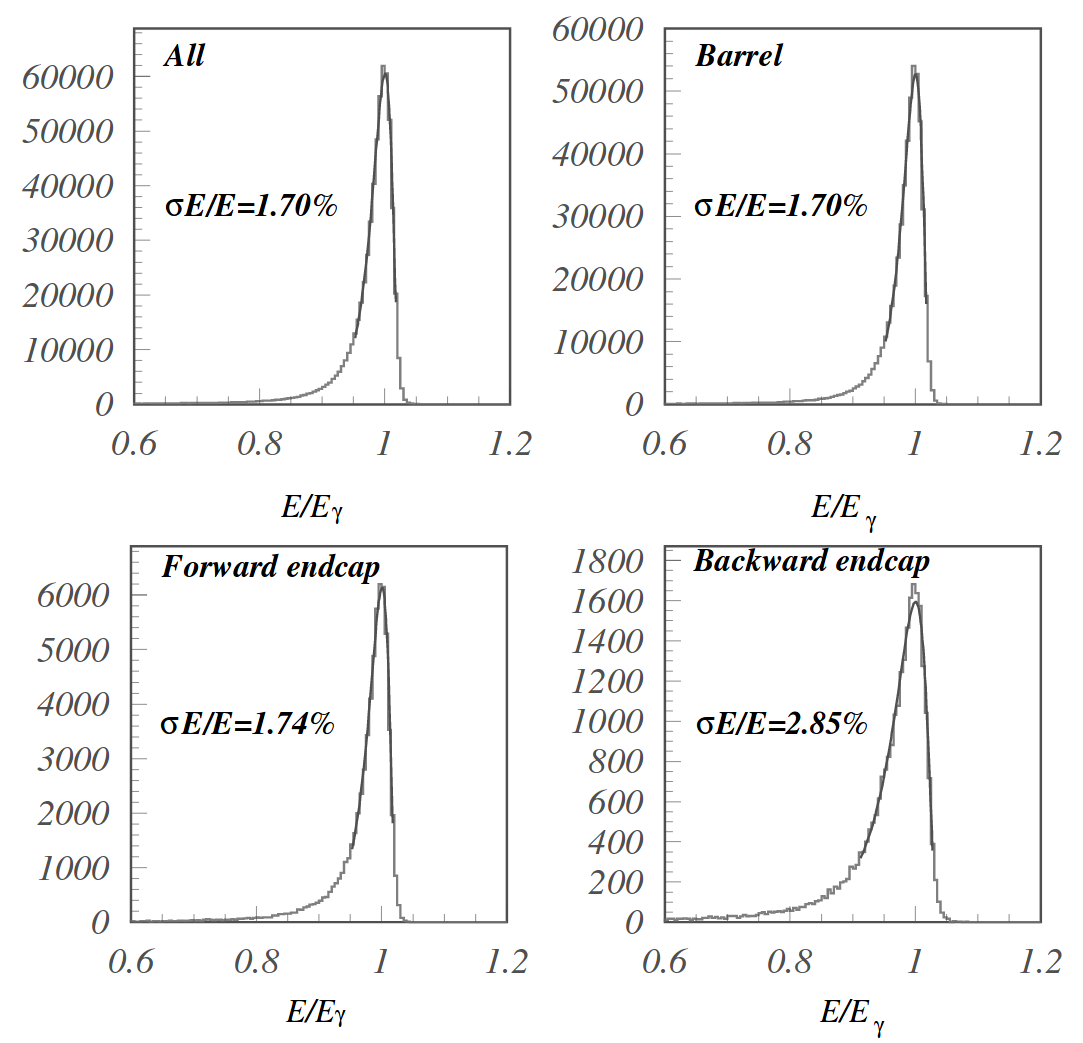
\includegraphics[width=0.8\linewidth]{fig/setup/ECL_resolution}
	\caption{Reconstructed energy distribution for $e^+e^- \to \gamma\gamma$ events for overall, barrel, forward and backward end-cap calorimeters \cite{ABASHIAN2002117}.}
	\label{fig:ECL_resolution}
\end{figure}

\subsection{$K_L^0/\mu$ Detector}
The KLM detector is used for detection of high-penetration particles such as $K_L^0$ and $\mu$ for momenta larger than $0.6\e{GeV}/c$. The setup covers the polar angle of $20^\circ < \theta < 155^\circ$. Detection of $K_L^0$ particles is troublesome since they are neutral and have a small material interaction probability, therefore a lot of material is needed in the KLM. To provide detection of both kinds of particles, hadronic and neutral, as well as electromagnetically and hadronically interacting, the KLM is constructed as a sampling calorimeter, which consists of 15 layers of $3.7\e{cm}$ thick resistive-plate counters (RPC) with 14 layers of $4.7\e{cm}$ thick iron plates between them. A single RPC module consists of two parallel plate electrodes, two glass panels, and gas in between. A charged particle passing the gas gap initiates a local discharge of the plates, which in turn induces signal to record the time and location of ionization. This is possible since the resistivity of the glass surface is high, so the discharge occurs locally. Hadrons interacting with the iron plates may produce a shower of ionizing particles, which are then also detected by the RPCs. The KLM is located outside of the superconducting solenoid and the iron plates of the KLM serve a dual role as the flux return for the magnetic field. Figure \ref{fig:KLM_layer} shows a cross-section of an RPC superlayer, consisting of an RPC pair.

\begin{figure}[!htb]
	\centering
	\captionsetup{width=0.8\linewidth}
	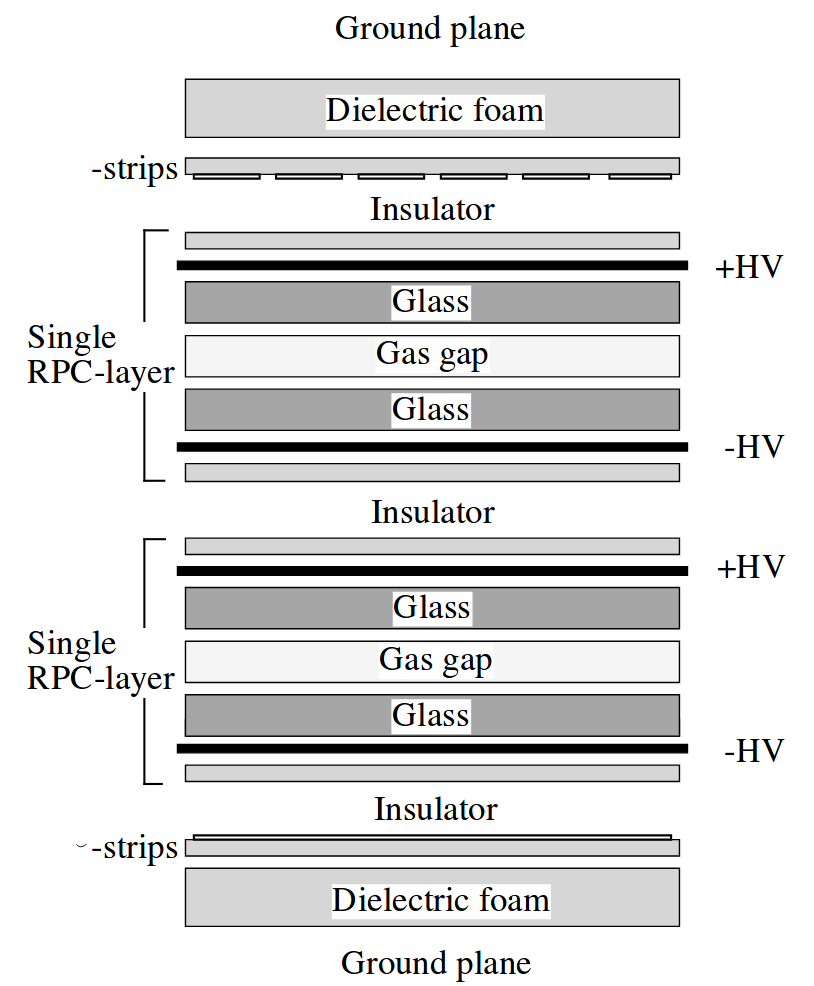
\includegraphics[width=0.5\linewidth]{fig/setup/KLM_layer}
	\caption{Cross-section of an RPC superlayer, consisting of an RPC pair \cite{ABASHIAN2002117}.}
	\label{fig:KLM_layer}
\end{figure}

The $K_L^0$ particle can be distinguished from other charged hadrons because they have no matched track in the CDC. The flight direction can also be inferred from the hit locations in the consecutive RPCs. Tracks of charged particles measured in CDC are extrapolated into KLM and clusters within $15^\circ$ of an extrapolated charged particle track are excluded from $K_L^0$ cluster candidates. On the other hand, muons with matched CDC tracks are able to reach the KLM if their momentum is larger than $0.5\e{GeV}/c$. They do not interact strongly and do not produce hadronic showers in the KLM, which serves as a handle on the muon identification. Figure \ref{fig:KLM_eff} (left) shows the number of neutral clusters per event and a Monte Carlo simulation of the predicted number of $K_L^0$ clusters per event. The average number of $K_L^0$ clusters per event is $0.5$. The agreement with the prediction gives us the confidence that the detector and our reconstruction software are performing correctly. Figure \ref{fig:KLM_eff} (right) shows the muon detection efficiency as a function of momentum and shown for a likelihood cut of $0.66$, where muon likelihood is based on the comparison of the measured range of a particle with the predicted range for a muon. Based on $K_S \to \pi^+\pi^-$ events, a muon identification efficiency of better than $90\%$ is determined,  with a pion fake rate of less than $5\%$ for particles with momenta more than $1.5\e{GeV}/c$ and a likelihood cut of $0.66$.

\begin{figure}[!htb]
	\centering
	\captionsetup{width=0.8\linewidth}
	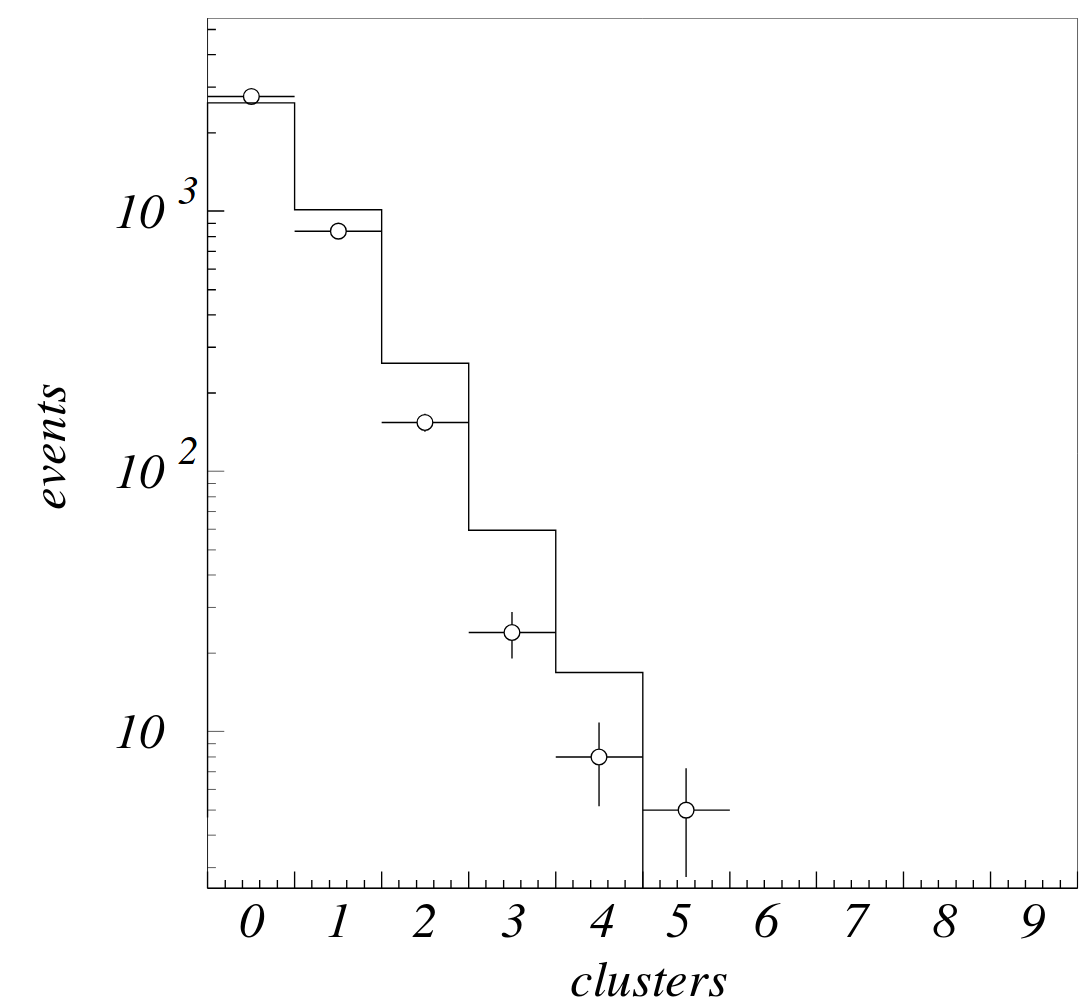
\includegraphics[width=0.48\linewidth,trim = 0cm -1.5cm 0cm 0cm]{fig/setup/KLM_clusters}
	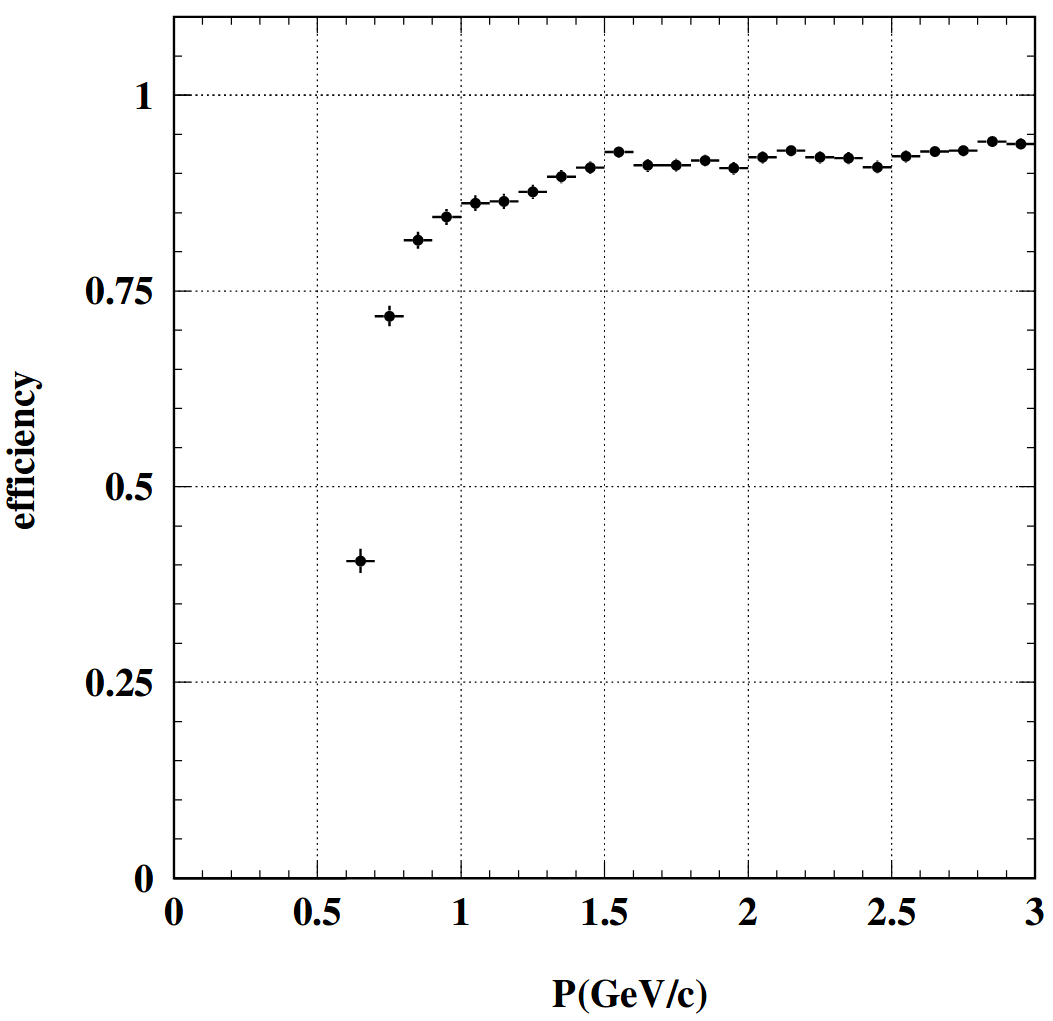
\includegraphics[width=0.48\linewidth]{fig/setup/KLM_efficiency}
	\caption{Number of neutral clusters per event in KLM (left) and muon detection efficiency as a function of momentum in KLM (right) \cite{ABASHIAN2002117}.}
	\label{fig:KLM_eff}
\end{figure}

Cosmic ray events have been used to determine the efficiency and resolution of the KLM, with an overall efficiency typically over $98\%$. The temporal and spatial resolutions of the KLM are few$\e{ns}$ and about $1.2\e{cm}$, respectively. The latter corresponds to an angular resolution from the interaction point of better than $10\e{mrad}$.

In order to do detector calibration and proper luminosity measurements, we need to accumulate samples of Bhabha and $\gamma\gamma$ scattering. Otherwise, as shown in Table \ref{tab:xsec}, the cross-section for physics events of interest is reasonably small. During normal operation (luminosity of $L = 10\E{34}\e{cm^{-2}s^{-1}}$) the total event rate is around $200\e{Hz}$, which is well below the data acquisition (DAQ) limit of $500\e{Hz}$. Out of this rate, $100\e{Hz}$ are physically interesting events, which include also two-photon events, Bhabha scattering, and $\mu$ pair production, besides hadronic events from $B \bar B$ pair events. In order to discard events which are not interesting for physics analyses, we use a trigger system by appropriately applying restrictive conditions. This section describes the necessary procedures and equipment to successfully do so.

\subsection{Trigger System}
The trigger system operates by immediately eliminating events that are not of interest, so that the amount of stored data is within the $500\e{Hz}$ frequency limit, while the efficiency for physics events of interest is kept high. Events which pass the triggers are then stored, otherwise discarded. The Belle trigger system consists of three stages, Level-1 (L1) online hardware trigger, Level-3 (L3) online software trigger and Level-4 (L4) offline software trigger.

L1 trigger is the first stage of the trigger system, which consists of multiple sub-detector triggers, all connected to a central trigger system called the Global Decision Logic (GDL), as schematically shown in Figure \ref{fig:TRG_GDL}. Each sub-detector trigger works on a principle of either a track trigger or an energy trigger. In the former case, the triggers discard events not meeting conditions based on the number of reconstructed tracks or track hits, while the latter is based on the total energy deposit and counting of crystal hits. Each sub-detector processes the event information and provides it to the GDL, where all the information is combined and the current event is characterized. The information from the sub-detector triggers reaches the GLD within $1.85\e{\mu s}$ after the collision, and the final trigger signal is provided within at a fixed $2.2\e{\mu s}$ latency. The combined efficiency from the L1 trigger is greater than $99.5\%$ for hadronic events.

\begin{figure}[!htb]
	\centering
	\captionsetup{width=0.8\linewidth}
	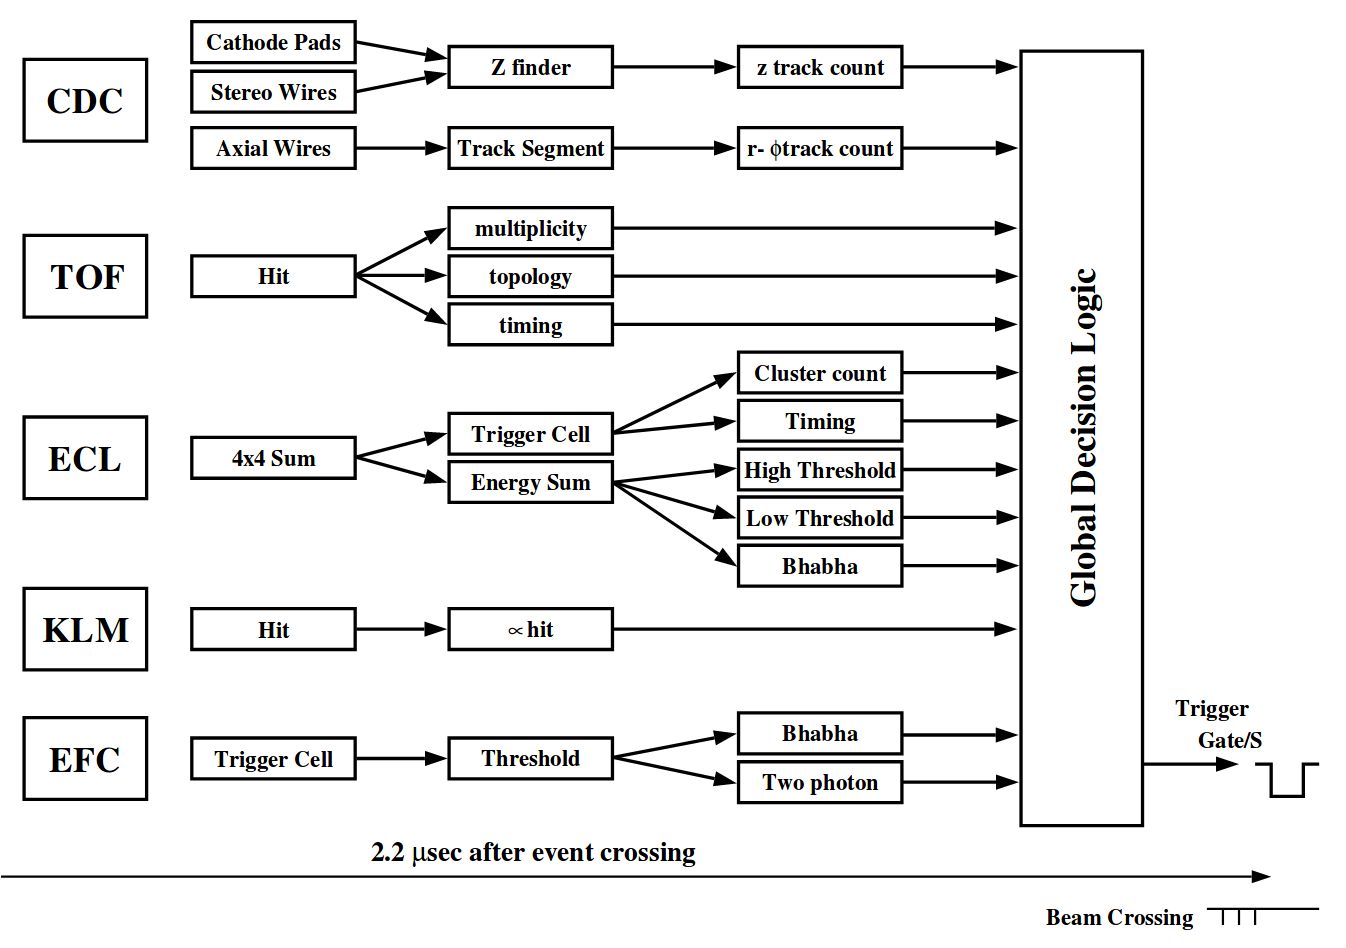
\includegraphics[width=0.8\linewidth]{fig/setup/TRG_GDL}
	\caption{The Level-1 trigger system for the Belle detector \cite{ABASHIAN2002117}.}
	\label{fig:TRG_GDL}
\end{figure}

After passing L1 trigger, the L3 discards background events from the software-wise perspective. L3 is an online software trigger which performs a simple, but fast reconstruction of the event. Events with at least one track satisfying the impact parameter condition $\vert\mathrm{d}z \vert < 5.0\e{cm}$ and with a total energy deposit in the ECL more than $1\e{GeV}/c$ are selected. The L3 trigger reduces the event rate by $50\%$, with a $99\%$ efficiency for hadronic events.

After passing the L3 trigger, the events are recorded on tapes. However, these data still contain many events from the beam background. To reduce the background events even further, they are required to pass the L4 offline software filtering. At the same time, high efficiencies for signal events is still required. Events must satisfy the following conditions
\begin{itemize}
	\item have at least one track with $p_T > 300\e{MeV}/c$ and impact parameters $\vert \mathrm{d}r \vert < 1.0\e{cm}$ and $\vert \mathrm{d}z \vert < 4.0\e{cm}$,
	\item have total energy deposit in the ECL must greater than $4\e{GeV}$.
\end{itemize}
Approximately $27\%$ of triggered events are passed through L4 while keeping an almost full efficiency for hadronic events. Events that pass the L4 trigger are fully reconstructed and stored to the DST. Overall, the efficiency of hadronic events after all trigger stages is measured to be more than $99\%$, which is more than the requirements from physics analyses.




\chapter{Belle to Belle II Format Conversion}

\section{Conversion Procedure}
The Belle experiment finished its data-taking run of 10 years at the end of 2010 after collecting a dataset of about $1\e{ab^{-1}}$. That year the Belle detector was shut down and the Belle II experiment has started in its place. While the focus moved to the construction of the Belle II detector and the development of the Belle II Analysis Framework (BASF2) \cite{Kuhr:2018lps}, Belle analyses are still on-going and Belle data is still being used today. BASF2 software with its modular structure has a more intuitive approach to performing analyses, however, since it was rewritten completely from scratch, it was designed for the incoming Belle II data and therefore out-of-the-box usage of Belle data is outside of its scope.

In the Belle Collaboration, a task force was created in order to convert Belle data into Belle II format (\btbii) \cite{Keck:b2bii2018}. The \btbii~package was developed as a part of BASF2 in order to convert data and MC of the Belle experiment and make it available within BASF2. In addition to the convenience of Belle data being processed in the more intuitive and advanced BASF2 framework, \btbii~allows for estimation and validation of performances of various advanced algorithms being developed for Belle II. The conversion itself, however, is considered non-trivial. Although the conversion of the raw detector data would be possible, the reconstruction algorithms of BASF2 are optimized for Belle II and cannot be effectively applied to Belle data. To bypass this problem, reconstructed objects from \texttt{PANTHER} tables, a custom solution of the Belle collaboration based on C/C++ and Fortran, are mapped to their corresponding representations in BASF2. In this analysis, we use the developed converter package in order to analyze Belle data with the Belle II software.

The conversion in the \btbii~package is divided into three BASF2 modules. The first module opens the Belle input files and reads the events into memory in the form of \texttt{PANTHER} tables. This module consists predominantly of reused BASF code. The second module applies various calibration factors, such as experiment- and run-dependent factors, to the beam energy, particle identification information, error matrices of the fitted tracks, etc. The module also applies some low-level selection criteria to reproduce removing background events as done within BASF. The actual conversion and the mapping of reconstructed objects are done in the last module. For more information see \cite{Keck:48940}.

\section{Validation}

In order to make sure the conversion was successful and without errors, a thorough validation should be performed. This is done by comparing histograms of all physical quantities of the reconstructed objects on simulated and recorded events, processed with BASF and BASF2. 

Our signal decay mode consists of three charged tracks, track conversion should perform flawlessly. Additionally, energy measurement is also very important in our untagged analysis in order to successfully determine the missing 4-momentum in the event, which is why we also need a correct conversion of the ECL clusters for photons and $\pi^0$ particles. Figures \ref{fig:b2bii_tracks} to \ref{fig:b2bii_pi0s} show the basic physical properties of converted tracks, photons and $\pi^0$ particles, obtained with BASF and BASF2, and their difference, which is (up to numerical precision) equal to 0. The plots indicate that the conversion is successful in all aspects and we can proceed with the analysis in the framework of BASF2.

\begin{figure}[H]
	\centering
	\captionsetup{width=0.8\linewidth}
	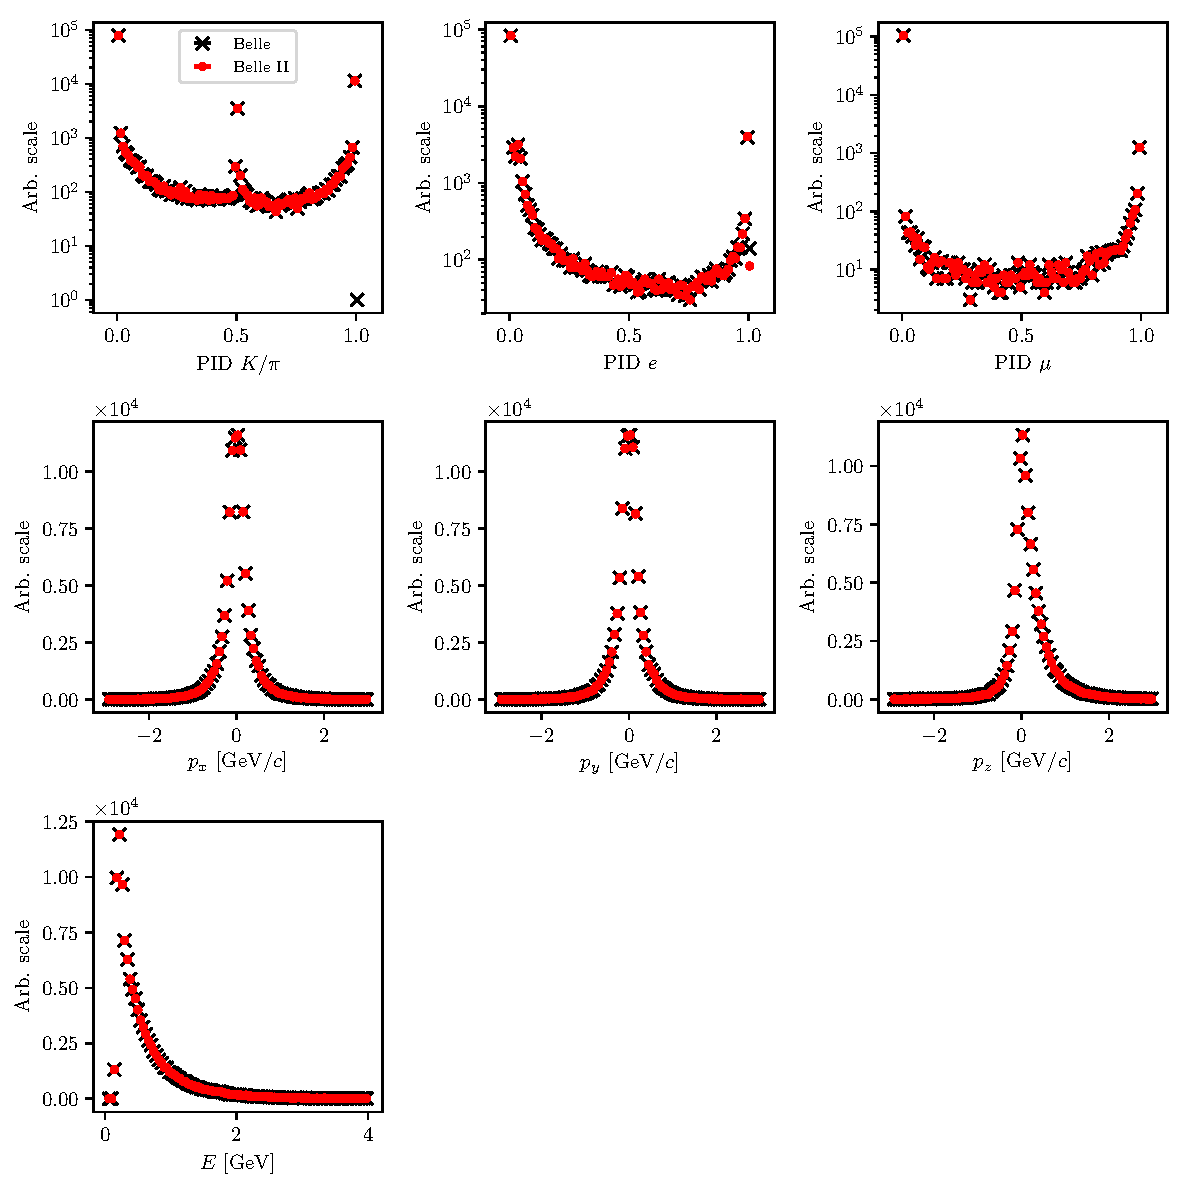
\includegraphics[width=\linewidth]{fig/b2bii_tracks}
	\caption{Some of the more important physical properties of tracks for Belle and Belle II in the conversion process. The histograms seem to overlap and the conversion is assumed to be successful.}
	\label{fig:b2bii_tracks}
\end{figure}

\begin{figure}[H]
	\centering
	\captionsetup{width=0.8\linewidth}
	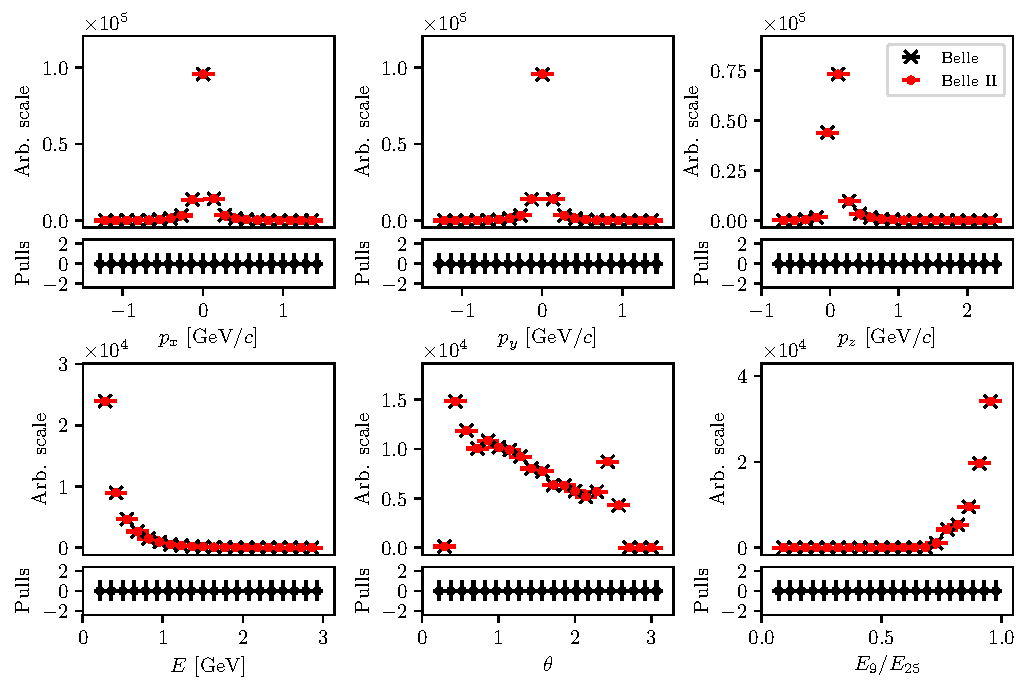
\includegraphics[width=\linewidth]{fig/b2bii_gammas}
	\caption{Some of the more important physical properties of photons for Belle and Belle II in the conversion process. The histograms seem to overlap and the conversion is assumed to be successful.}
	\label{fig:b2bii_gammas}
\end{figure}

\begin{figure}[H]
	\centering
	\captionsetup{width=0.8\linewidth}
	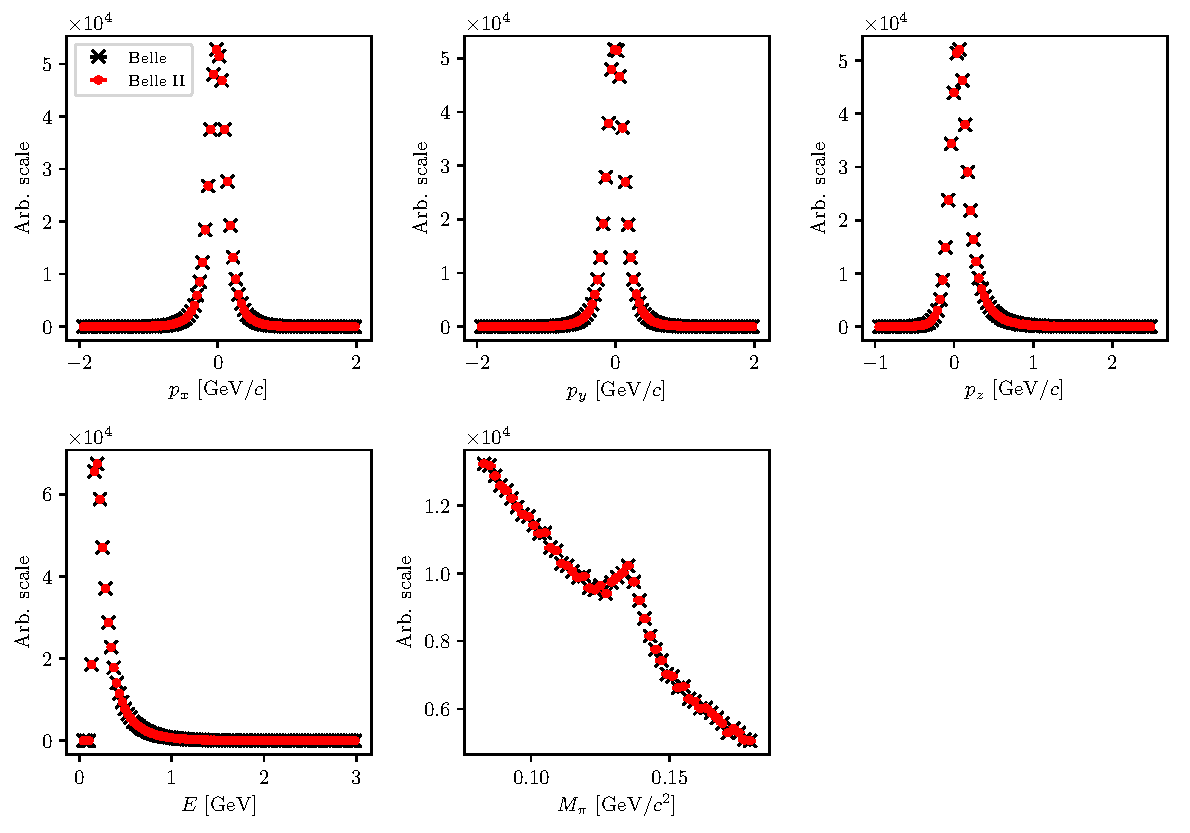
\includegraphics[width=\linewidth]{fig/b2bii_pi0s}
	\caption{Some of the more important physical properties of $\pi^0$ particles for Belle and Belle II in the conversion process. The histograms seem to overlap and the conversion is assumed to be successful.}
	\label{fig:b2bii_pi0s}
\end{figure}

%\section{Conversion improvement}
%
%An additional improvement is applied to neutral particles after the conversion where we change the origin of the ECL clusters to the interaction point instead of the point $(0,0,0)$, which was used at Belle. In order to successfully implement this improvement, we have to make sure that the conversion of the beam parameters is successful and how the momentum resolution of neutral particles changes after its implementation. Figure X shows the distributions of the beam parameters for Belle and Belle II, which shows no obvious errors in the conversion process. Improving the information about the origin point of photons then results in improvement of the momentum determination. The comparison is shown in Figure X with an obvious benefit after the mentioned implementation.
%
%PLOT
%
%PLOT
\chapter{Event reconstruction}

In this chapter the procedure for event reconstruction of the $B$ meson decay $B \to K K \ell \nu$ is shown, starting with final state particle selection and then combining them to obtain $B$ meson candidates.

\section{Final state particles selection}
Since the neutrino escapes detection, we can only reconstruct the charged tracks in the decay, which are the two charged kaons ($K$) and the light lepton, which is the electron ($e$) or muon ($\mu$). These are some of the particles which are commonly referred to as final state particles (FSP). Final state particles have a long lifetime and are usually the particles that we detect when they interact with the material in the detector.

It is important to limit our selection of FSP particles in order to cut down the number of particle combinations, and consequentially computation time and file sizes.

\subsubsection{Leptons}

Figures \ref{fig:evars} and \ref{fig:muvars} show the impact parameters $d_0$ and $z_0$, the momentum in  $\Upsilon(4S)$ center-of-mass system (CMS), and the PID information for true and fake electrons and muons, where an extra category for true electrons/muons from the signal decay is shown.

\begin{figure}[H]
\centering
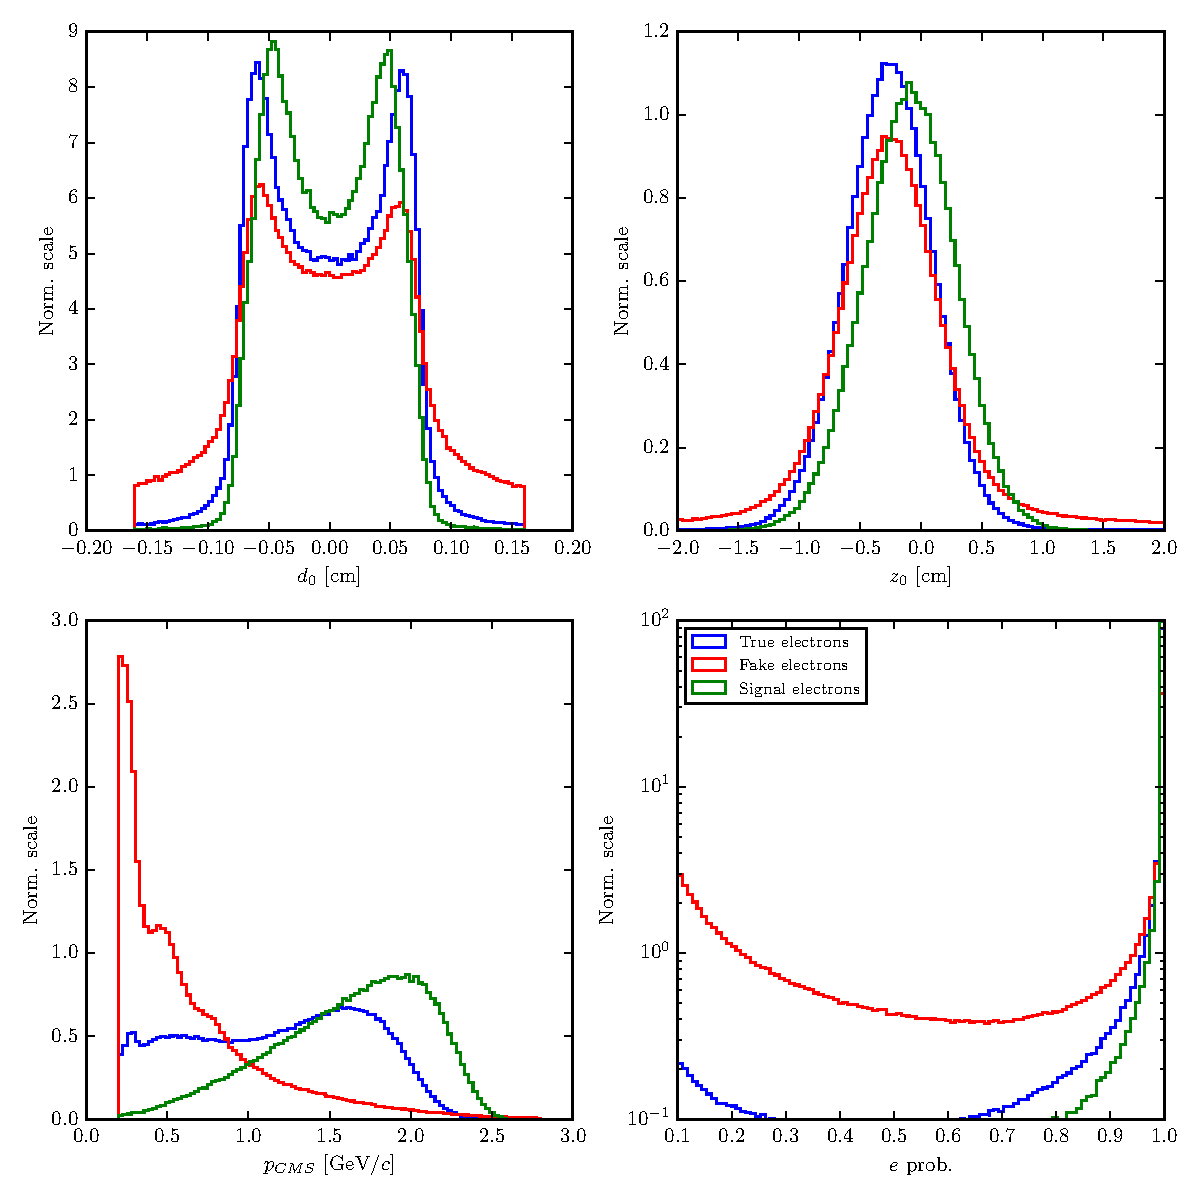
\includegraphics[width=\linewidth]{fig/FSP_e_vars}
\captionsetup{width=.8\linewidth}
\caption{Normalized properties of true (blue), fake (red) and true electrons from signal $B$ candidates (green).}
\label{fig:evars}
\end{figure}

\begin{figure}[H]
\centering
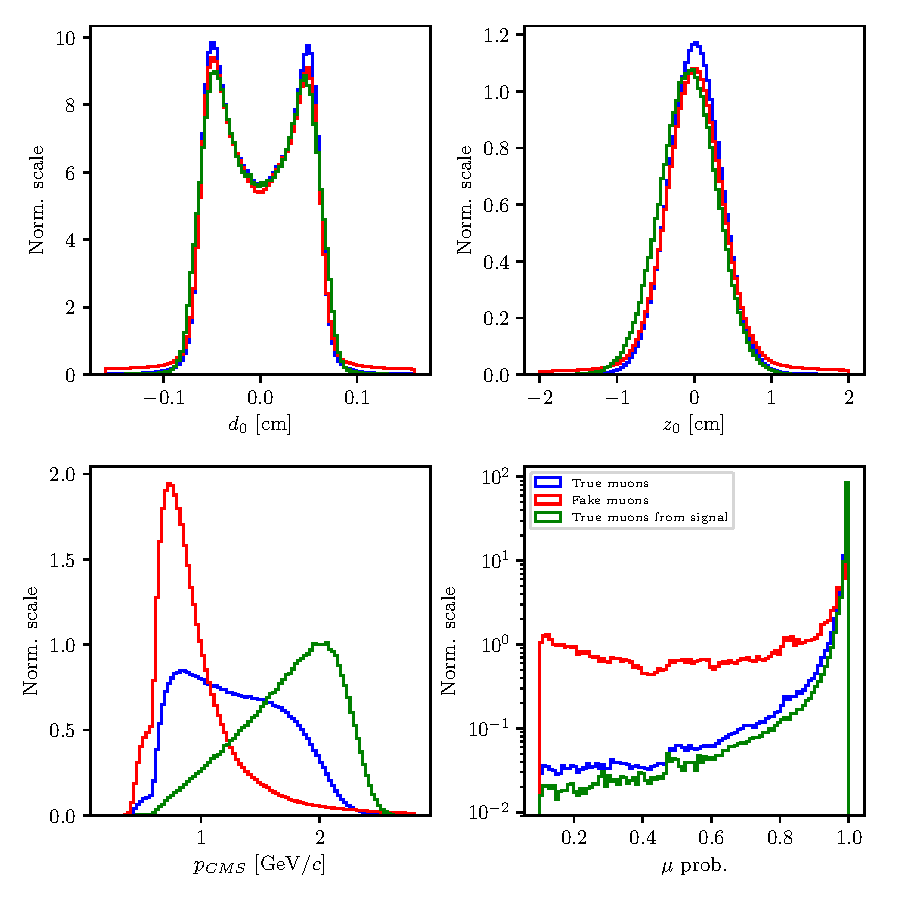
\includegraphics[width=\linewidth]{fig/FSP_mu_vars}
\captionsetup{width=.8\linewidth}
\caption{Normalized properties of true (blue), fake (red) and true muons from signal $B$ candidates (green).}
\label{fig:muvars}
\end{figure}

Based on these distributions, we can define a set of cuts
\begin{itemize}
\item $\vert d_0 \vert < 0.1\e{cm}$,
\item $\vert z_0 \vert < 1.5\e{cm}$,
\item $p_{CMS} \in [0.4,\,2.6]~\e{GeV}/c$ for electrons,
\item $p_{CMS} \in [0.6,\,2.6]~\e{GeV}/c$ for muons.
\end{itemize}

After this selection we can determine the optimal PID cuts for electrons and muons, where we optimize the selection by maximizing the standard definition of \textit{figure of merit} ($\mathrm{FOM}$), defined in Eq. (\ref{eq:fom})
\begin{equation}
\label{eq:fom}
\mathrm{FOM} = \sqrt{\mathcal{E}\mathcal{P}} \propto \frac{S}{\sqrt{S+B}},
\end{equation} 
where the argument in the square root is the product of the efficiency ($\mathcal{E}$) and the purity ($\mathcal{P}$) function. The definitions of signal ($S$) and background ($B$) are somewhat fluid throughout the analysis and need to be defined for each $\mathrm{FOM}$ separately. In this section we define two representations of $S$ and $B$. In $\mathrm{FOM}_1$ the signal $S$ represents correctly reconstructed final state particles, while in $\mathrm{FOM}_2$ the signal $S$ represents correctly reconstructed final state particles which also come from a correctly reconstructed $B$ meson candidate. In both cases $B$ represents all other particle candidates which do not satisfy the conditions of $S$.

The $\mathrm{FOM}$ plots are shown in Figures \ref{fig:efom} and \ref{fig:mufom}. The cut values are based on PID cuts used for PID efficiency calibration. The optimal value for the PID cuts is equal to the largest available value, regardless of the leptons coming from signal decays or not. The optimized PID cuts for leptons are
\begin{itemize}
\item $e$ prob. $ > 0.9$ for electrons,
\item $\mu$ prob. $ > 0.97$ for muons.
\end{itemize}

\begin{figure}[H]
\centering
\captionsetup{width=.8\linewidth}
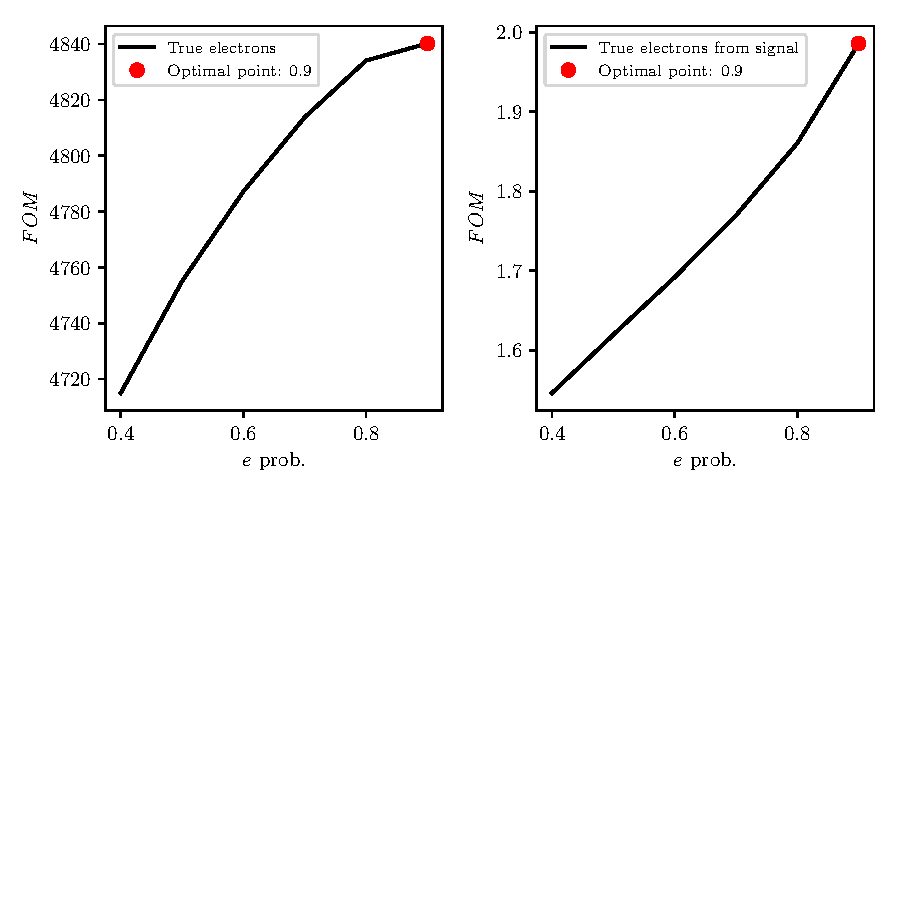
\includegraphics[width=\linewidth]{fig/FSP_e_fom}
\caption{$\mathrm{FOM}$ optimizations of the PID probability cuts for true electrons (left) and true electrons from signal $B$ candidatess (right).}
\label{fig:efom}
\end{figure}

\begin{figure}[H]
\centering
\captionsetup{width=.8\linewidth}
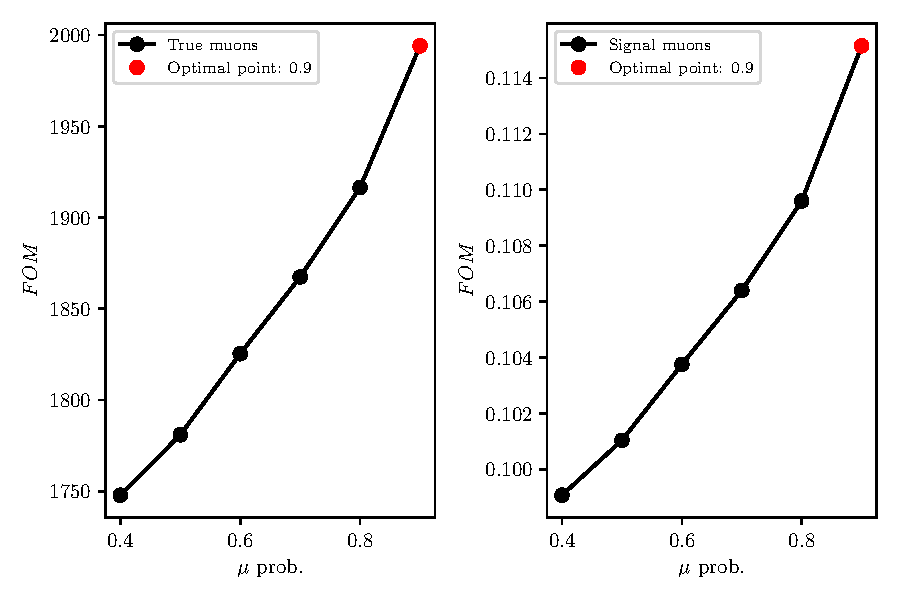
\includegraphics[width=\linewidth]{fig/FSP_mu_fom}
\caption{$\mathrm{FOM}$ optimizations of the PID probability cuts for true muons (left) and true muons from signal $B$ candidates (right).}
\label{fig:mufom}
\end{figure}


\subsubsection{Kaons}

We repeat the procedure for both kaons. Figure \ref{fig:Kvars} shows the impact parameters $d_0$ and $z_0$, the momentum in  $\Upsilon(4S)$ center-of-mass system (CMS), and the PID information for true and fake kaons, where an extra category for true kaons from the signal decay is shown.

\begin{figure}[H]
\centering
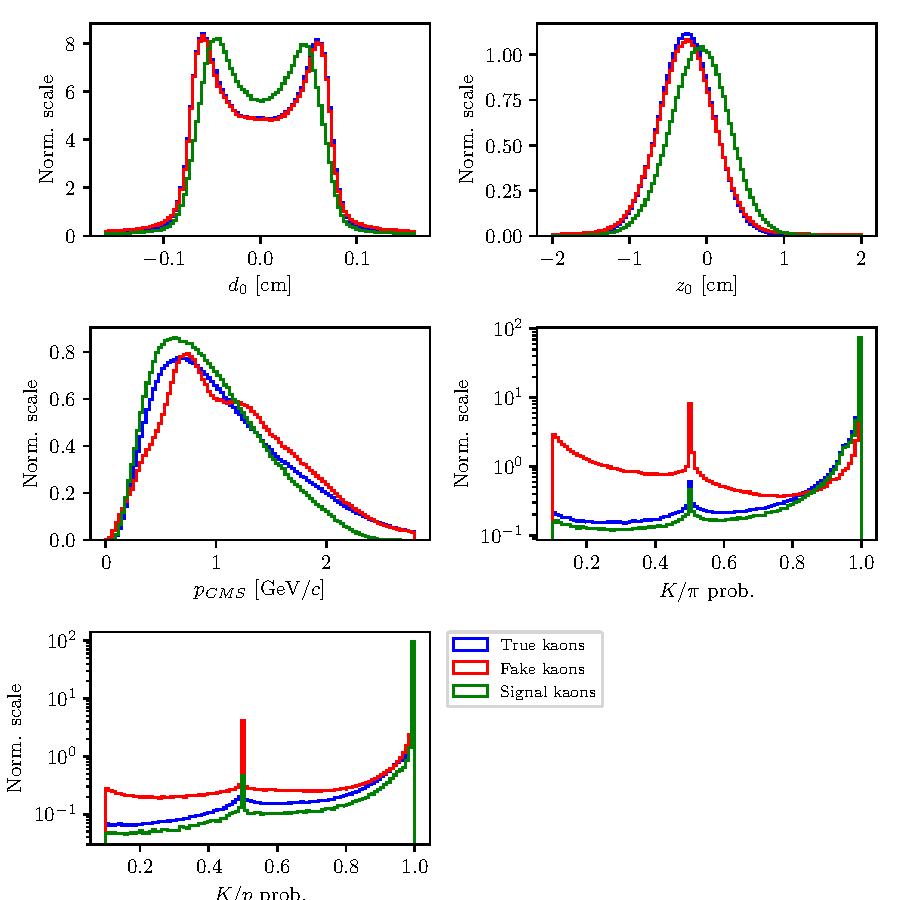
\includegraphics[width=\linewidth]{fig/FSP_kaon_vars}
\captionsetup{width=.8\linewidth}
\caption{Normalized properties of true (blue), fake (red) and true kaons (green) from signal $B$ candidates.}
\label{fig:Kvars}
\end{figure}

We define the kaon cuts in the same manner as in the case for leptons
\begin{itemize}
\item $\vert d_0 \vert < 0.15\e{cm}$,
\item $\vert z_0 \vert < 1.5\e{cm}$,
\item $p_{CMS} \in [0,\,2.5]~\e{GeV}/c$.
\end{itemize}

The PID optimization in this case is taken in two steps. First we optimize the cut on $K / \pi$, and after that the $K/p$ separation probability. Figure \ref{fig:Kfom} shows the optimization procedure for PID cuts on kaon candidates.

\begin{figure}[H]
\centering
\captionsetup{width=.8\linewidth}
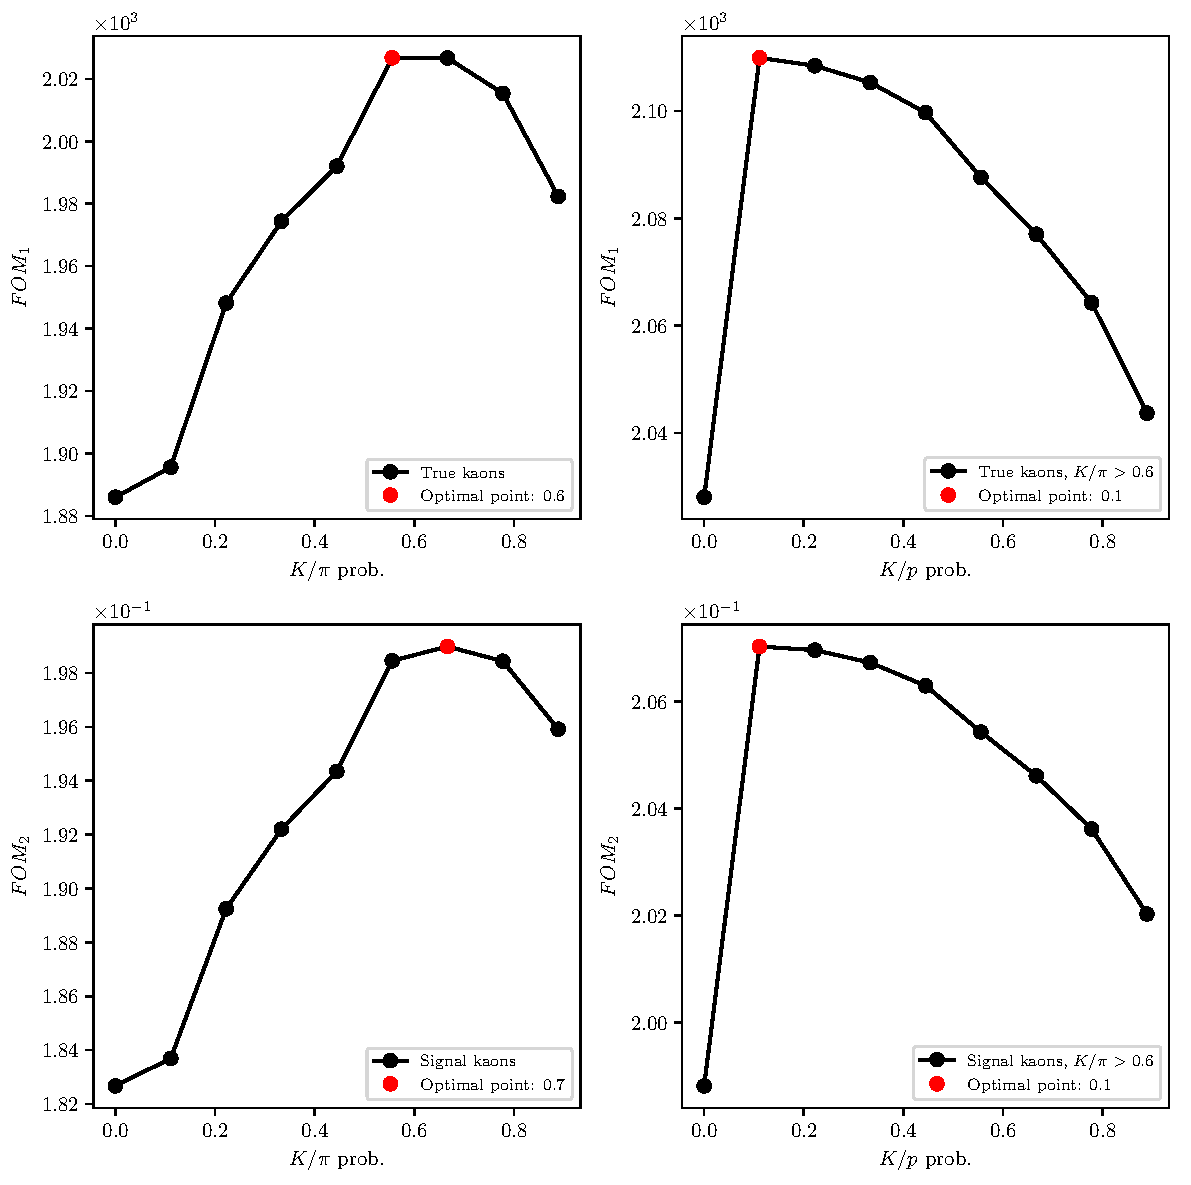
\includegraphics[width=\linewidth]{fig/FSP_kaon_fom}
\caption{$\mathrm{FOM}$ optimizations of the PID probability cuts for true kaons (top) and true kaons from signal $B$ candidates (bottom). The plots on the left show the optimization of the first step for the $K / \pi$ probability cut, and the plot on the right the $K/p$ probability cut.}
\label{fig:Kfom}
\end{figure}

The optimized PID cuts for kaons are
\begin{itemize}
\item $K/\pi > 0.6$,
\item $K/p > 0.1$.
\end{itemize}

\section{Combination of FSP particles}

With the pre-selected kaon and lepton candidates we make combinations for potential $B$ meson candidates. Since the missing neutrino escapes detection, we reconstruct the $B$ mesons in the following two channels
\begin{align*}
B^+ &\to K^+ K^- e^+, \\
B^+ &\to K^+ K^- \mu^+,
\end{align*}
and similarly for $B^-$. When an arbitrary combination is obtained, we perform a vertex fit of the three tracks in order to discard combinations with a low probability of tracks coming from the same point. $B$ mesons have a relatively long lifetime and decay along the $z$ axis of the detector in the direction of the boost, so the vertex fit is enforced with an \texttt{IPTUBE} constraint, which constrains the vertex to an elongated ellipsoid along beam direction. We demand that the fit converged and apply a cut on the minimal fit probability. The fit probability for signal and background $B$ meson candidates is shown in Figure \ref{fig:vtx} (left). We perform a $\mathrm{FOM}$ cut optimization of this variable, which is shown in Figure \ref{fig:vtx} (right). In this and in the following cases, the definition of $S$ from Eq. (\ref{eq:fom}) are correctly reconstructed $B$ meson candidates with a missing neutrino which are not coming from the $b \to c$ transition.

\begin{figure}[H]
\centering
\captionsetup{width=0.8\linewidth}
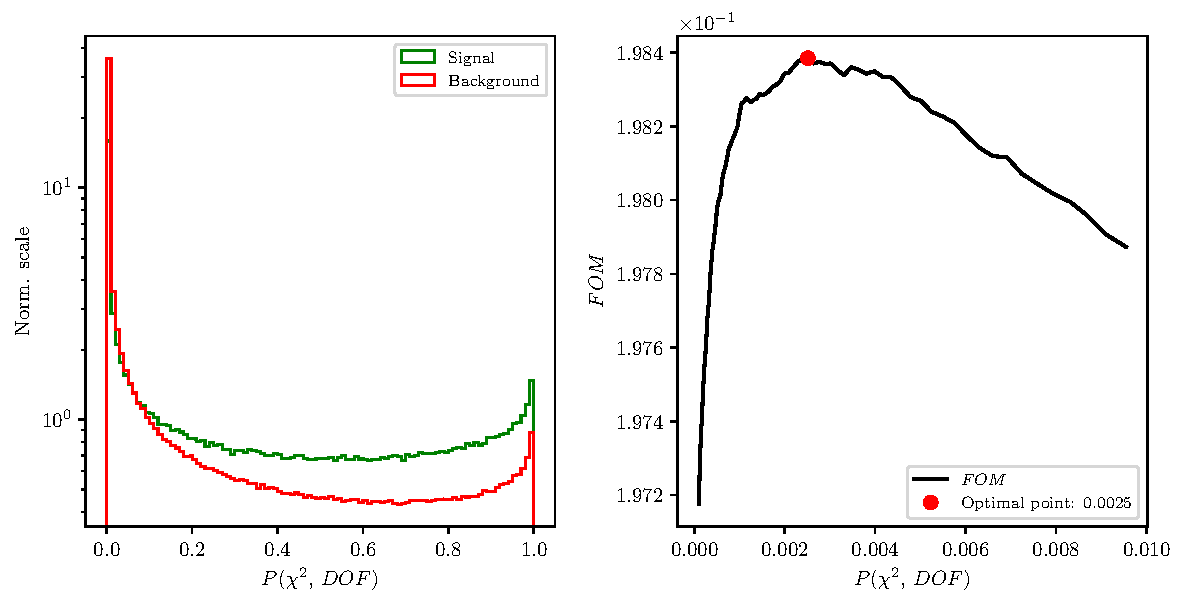
\includegraphics[width=\linewidth]{fig/VTX}
\caption{Normalized vertex fit probability distribution for signal and background $B$ meson candidates in logarithmic scale (left) and $\mathrm{FOM}$ optimization of the vertex fit probability (right).}
\label{fig:vtx}
\end{figure}

Even though the vertex fit probability cut was optimized, we choose a slightly different but a more standard cut of
\begin{itemize}
\item $P(\chi^2,NDF) > 1.0\E{-3}$.
\end{itemize}

With the neutrino being the only missing particle on the reconstructed side, it is possible to determine the angle between the direction of the reconstructed $B$ (denoted as $Y \to K K \ell$) and the nominal $B$, as
\begin{align}
\mathrm{p}_\nu &= \mathrm{p}_B - \mathrm{p}_{Y}, \\
\label{eq:massnu}
\mathrm{p}_\nu^2 = m_\nu^2 &= m_B^2 + m_Y^2 - 2E_BE_Y + 2\vec{p}_B \cdot \vec{p}_Y \approx 0, \\ 
\label{eq:cosby}
\cos \left(\theta_{BY}\right) &= \frac{2E_BE_Y - m_B^2 - m_Y^2}{2\vert \vec{p}_B \vert \vert \vec{p}_Y\vert},
\end{align} 

where all the energy and momenta above are calculated in the CMS frame. The mass of the neutrino is equal to 0 to a very good precision, so we use it in Eq. (\ref{eq:massnu}). In addition, we can substitute the unknown energy and momentum magnitude, $E_B$ and $\vert \vec{p}_B \vert$, of the $B$ meson in Eq. (\ref{eq:cosby}), with quantities from the well known initial conditions
\begin{align}
E_B &= E_{CMS} / 2,\\
\vert \vec{p}_B \vert = p_B &= \sqrt{E_B^2 - m_B^2},
\end{align} 

where $E_{CMS}$ is the total energy of the $e^+e^-$ collision in the CMS frame and $m_B$ is the nominal mass of the $B$ meson. 

For the correctly reconstructed candidates, this variable lies in the $[-1,1]$ region, though only to a certain precision, due to the finite detector resolution. For background candidates, however, the candidates populate also the non-physical regions, as shown in Figure \ref{fig:cosby} (left). We impose an optimized cut on this variable from Figure \ref{fig:cosby} (right) to discard a large amount of background.
\begin{itemize}
\item $\vert \cos \left(\theta_{BY}\right) \vert < 1.0$.
\end{itemize}

\begin{figure}[H]
\centering
\captionsetup{width=.8\linewidth}
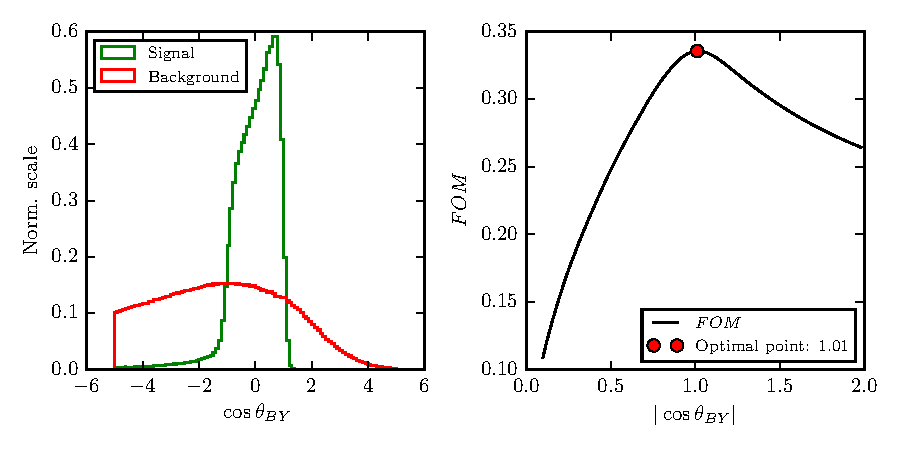
\includegraphics[width=\linewidth]{fig/cosBY}
\caption{Normalized $\cos \theta_{BY}$ distribution for signal and background $B$ meson candidates (left) and $\mathrm{FOM}$ optimization of the $\cos \theta_{BY}$ variable (right).}
\label{fig:cosby}
\end{figure}

\section{Loose neutrino reconstruction}\label{sec:loose-neutrino-reconstruction}

%Due to the beam background in the detector, material interactions, or other processes, random tracks and clusters enter our event and get reconstructed as part of the physics process we want to study. These tracks and clusters are not interesting and further spoil the data we measure. In order to remedy this, we perform an extensive clean-up of the tracks and clusters in the ROE side before calculating the four-momentum of the missing part of the event. The clean-up procedure is performed separately on tracks and clusters and uses multiple steps with multivariate analysis (MVA) algorithms in order to separate good tracks and clusters from the bad ones, which populate the ROE. Then, for each ROE object, a ROE mask is created for tracks and clusters, which narrates the use of this track or cluster in the final calculations of the ROE four-momentum.
%
%In order to preserve the continuity of this chapter, a more detailed description of the ROE clean-up can be found in Chapter \ref{ch:roe}. From this point on we assume the ROE to be efficiently cleansed of extra tracks and clusters .


The signal-side neutrino escapes detection, so we cannot directly determine it's four-momentum. However, due to the detectors geometry, which almost completely covers the full solid angle, and due to well known initial conditions of the $\Upsilon(4S)$ meson, it is possible to determine the kinematics of the missing neutrino via indirectly reconstructing the companion $B$ meson by summing up the four-momenta of all the FSP particles in the event which were not used in the reconstruction of the signal side $B$ meson. This is known as the \textit{untagged} method since we are not using any kind of tagging method to reconstruct the companion $B$ meson. The particles used in the indirect companion $B$ meson reconstruction are also said to belong to the \textit{rest of the event} (ROE).

Due to the beam background in the detector, material interactions, or other processes, random tracks and clusters enter our event and get reconstructed as part of the physics process we want to study. These tracks and clusters are not interesting and further spoil the data we measure. In order to remedy this, we perform an extensive clean-up of the tracks and clusters in the ROE side before calculating the four-momentum of the missing part of the event. Here we see the motivation for the ROE clean-up, since our signal candidate reconstruction depends on tracks and clusters in the ROE side. The clean-up procedure is performed separately on tracks and clusters and uses multiple steps with multivariate analysis (MVA) algorithms in order to separate good tracks and clusters from the bad ones, which populate the ROE. Then, for each ROE object, a ROE mask is created for tracks and clusters, which narrates the use of this object in the final calculations of the ROE four-momentum. From this point on we assume the ROE to be efficiently cleansed of extra tracks and clusters. A more detailed description of the ROE clean-up can be found in Chapter \ref{ch:roe}. 

The total missing four-momentum in the event can be determined as
\begin{align}
\mathrm{p}_{miss} &= \mathrm{p}_{\Upsilon(4S)} - \sum_i^{\mathrm{Event}}\left(E_i,\,\vec{p}_i \right),\\
\label{eq:ROEloop}
\mathrm{p}_{miss} &= \mathrm{p}_{\Upsilon(4S)} - \left(\mathrm{p}_{Y} -\sum_i^{\mathrm{Rest~of~event}}\left(E_i,\,\vec{p}_i \right)\right),
\end{align}

where the summation runs over all charged and neutral particles in the defined set with
\begin{equation}
\mathrm{p}^{neutral}_i = \left(p_i,\, \vec{p}_i \right) \quad \mathrm{and} \quad \mathrm{p}^{charged}_i = \left(\sqrt{m_i^2 + p_i^2},\, \vec{p}_i \right),
\label{eq:pcharged}
\end{equation}
where we assumed all neutral particles to be massless photons. For charged tracks in the ROE a mass hypothesis needs to be defined in order to determine the track's energy. After the ROE clean-up we make the following procedure of choosing the mass hypothesis
\begin{enumerate}
\item $e$, if $e$ prob. $> \mu$ prob. and $e$ prob. $> 0.9$,
\item otherwise $\mu$, if $\mu$ prob. $> e$ prob. and $\mu$ prob. $> 0.97$,
\item otherwise $K$, if $K/\pi$ prob. $> 0.6$,
\item otherwise $\pi$.
\end{enumerate} 
We define the square of the missing mass, $m_{miss}^2$, which is consistent with zero, if signal-side neutrino is the only missing particle in the event, as shown in Eq. (\ref{eq:m2def}).
\begin{align}
\label{eq:nuold}
\mathrm{p}_\nu &= \mathrm{p}_{miss} = \left(E_{miss},\,\vec{p}_{miss} \right),\\
\label{eq:m2def}
m_{miss}^2 &= \mathrm{p}_{miss}^2 = \mathrm{p}_{\nu}^2 = m_\nu^2 \approx 0.
\end{align}

Since the detector is not perfect, the distribution of the $m_{miss}^2$ variable has a non-zero width. Additionally, tails are introduced as soon as we have missing particles such as extra missing neutrinos, other neutral undetected particles such as $K_L^0$, or simply missing tracks due to detection failure. Figure \ref{fig:missm2} shows the distribution of $m_{miss}^2$ as defined with the missing four-momentum in Eq. (\ref{eq:nuold}). Correctly reconstructed candidates, which come from events where the other $B$ meson decayed via a hadronic decay mode, should peak at zero. If this is not the case, candidates are shifted to larger values of this variable. Due to this fact, we impose a cut on the $m_{miss}^2$ variable in order to partially discard candidates with spoiled properties, even if it was in principle a correct combination of FSP particles on the signal side
\begin{itemize}
\item $\vert m_{miss}^2 \vert < 7\e{GeV}/c^2$.
\end{itemize}

For further purposes in this analysis we also define a subset of all signal candidates, which come from events where the companion $B$ meson decayed hadronically and all of it's particles were taken into account correctly. We only allow for missing photons, since they are frequently irradiated due to brehmsstrahlung effects and don't have such a big impact on the 4-momentum of the final candidate. We denote this subset as \textit{perfect} signal.

This cut on $m_{miss}^2$ was not optimized as the optimal case would result in a too strong threshold if optimized on perfect signal sample, since we still may want to retain as much signal candidates as possible, even if they are coming from events with semi-leptonic decays of the other $B$ meson.

\begin{figure}[H]
\centering
\captionsetup{width=.8\linewidth}
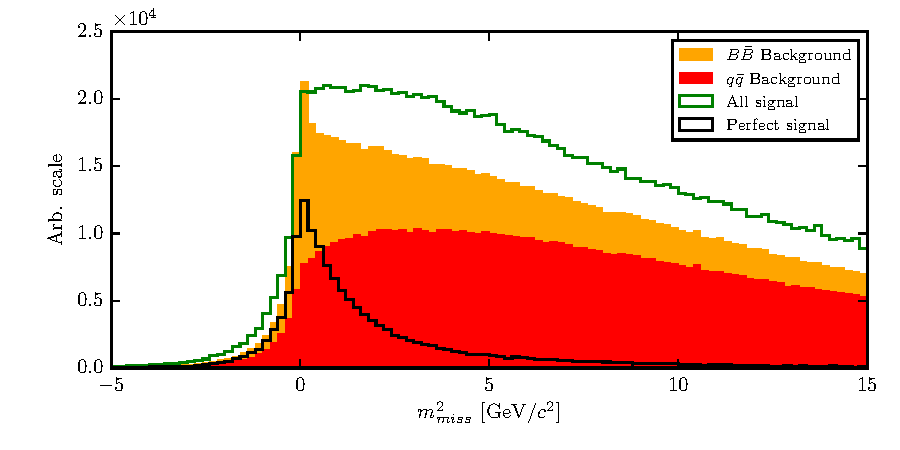
\includegraphics[width=\linewidth]{fig/missM2}
\caption{Squared missing mass distribution for $q \bar q$ and $B \bar B$ background in filled histograms. All signal (green) and perfect signal (black) are scaled up equally.}
\label{fig:missm2}
\end{figure}

The main uncertainty of the neutrino four-momentum, defined in Eq. (\ref{eq:nuold}), comes from energy uncertainty. It is a common practice to substitute the missing energy with the magnitude of the missing momentum, since the momentum resolution from the measurement is much better, thus redefining the neutrino four-momentum to
\begin{equation}
\label{eq:nunew}
\mathrm{p}_\nu = \left(\vert \vec{p}_{miss} \vert,\,\vec{p}_{miss} \right),
\end{equation}
which fixes the neutrino mass to $0\e{GeV}/c^2$.

The newly defined neutrino four-momentum can be added to the four-momentum of the $Y(KK\ell)$ candidate to obtain the full $B$ meson four-momentum and calculate the traditional $M_{BC}$ and $\Delta E$ variables
\begin{align}
\label{eq:de}
\Delta E &= E_B - E_{CMS}/2,\\
M_{BC} &= \sqrt{\left(E_{CMS}/2\right)^2 - \vert \vec{p} \vert^2}.
\end{align}

Since the final fit will be performed over \vars, we define the fit region
\begin{itemize}
\item $M_{BC} \in [5.1,\,5.295]\e{GeV}/c^2$,
\item $\Delta E \in [-1.0,\,1.3]\e{GeV}$.
%\item Signal enhanced region: $M_{BC} \in [5.27,\,5.295]\e{GeV}/c^2$ and $\vert \Delta E \vert < 0.143 \e{GeV}$,
\end{itemize}

Figure \ref{fig:mbc_de_pre} shows the distributions of $\Delta E$ (left) and $M_{BC}$ (right) for signal and major types of background after the pre-cuts. Both signal components are scaled up with respect to the background components, but are in proper scale one to another. The effects of missing particles are clearly seen based on the shape difference between all and perfect signal.

\begin{figure}[H]
\centering
\captionsetup{width=0.8\linewidth}
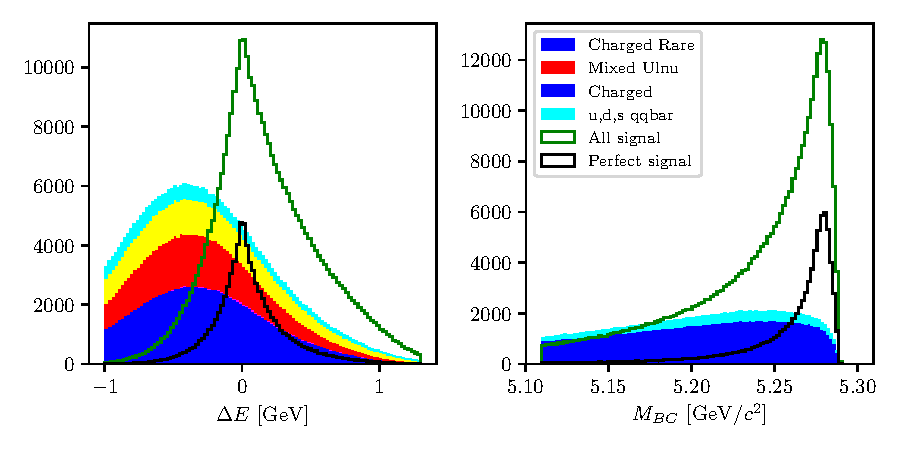
\includegraphics[width=\linewidth]{fig/mbc_de_pre}
\caption{Distributions of $\Delta E$ (left) and $M_{BC}$ (right) for signal and major types of background after the precuts. Both signal components are scaled up with respect to the background components, but are in proper scale one to another. The perfect signal has a much better resolution in both distributions, since the event is perfectly reconstructed.}
\label{fig:mbc_de_pre}
\end{figure}


%\section{$q^2$ calculation}
%
%Momentum transfer squared, $q^2$, is the squared Lorentz invariant of the four-momentum which is transferred from the $B$ meson to the $W$ boson. There are several possible calculations of this variable which offer different resolution. The following describes the calculation of $q^2$ which follows the calculation from [] and yields the best resolution.
%
%For correctly reconstructed events Eq. (\ref{eq:de}) satisfies the condition $\Delta E \approx 0$ within precision. It is possible to rescale the neutrino energy in such way that we fix $\Delta E$ to zero, meaning 
%\begin{equation}
%\Delta E' = (E_Y + \alpha E_\nu) - E_{CMS}/2 = 0.
%\end{equation}
%and calculate and adapted version of $M_{BC}$
%\begin{equation}
%M_{BC}' = \sqrt{\left(E_{CMS}/2\right)^2 - \vert \vec{p}_Y + \alpha \vec{p}_\nu \vert^2}.
%\end{equation}
%
%The neutrino momentum resolution dominates the $\Delta E$ uncertainty [], so the correction factor $\alpha$ reduces this source of uncertainty.
%
%A second correction can be applied by rotating the direction of the neutrino momentum by a small angle with respect to the reconstructed one. Such an angle is chosen in order fix the value of $M_{BC}'$ to the nominal mass of the $B$ meson, $m_B$.
%
%The corrected neutrino momentum is then solely used for the $q^2$ calculation, alongside the reconstructed lepton four-momentum, as
%\begin{equation}
%\label{eq:q2}
%q^2 = \mathrm{q}^2 = \left(\mathrm{p}_\ell + \mathrm{p}_\nu \right)^2.
%\end{equation}
%
%The $q^2$ distribution and its resolution are shown in Figure \ref{fig:q2}, along with additional versions of $q^2$, with details of the calculation method in the caption.
%\begin{figure}[H]
%\centering
%\captionsetup{width=0.8\linewidth}
%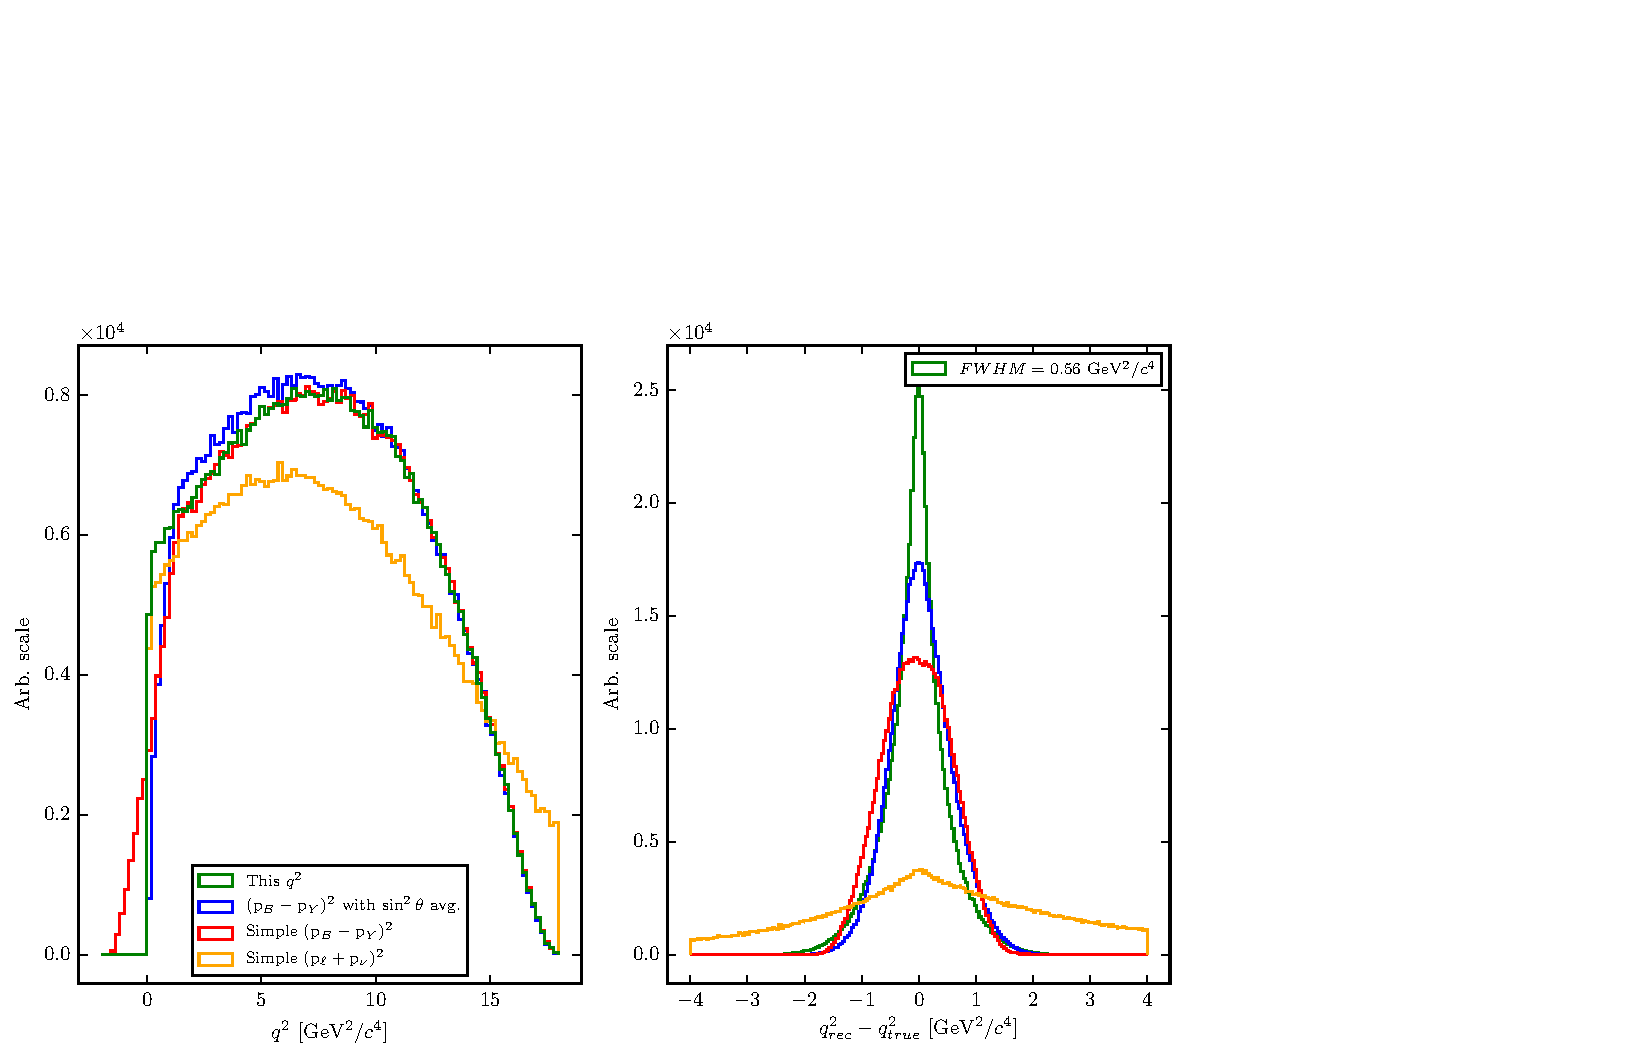
\includegraphics[width=\linewidth]{fig/q2}
%\caption{Distributions of $q^2$ (left) and $q^2$ resolution (right) for various methods of $q^2$ calculation. The blue distribution follows the procedure in [], whereas the red and the orange ones are straight-forward calculations with available information in the reconstruction. The $q^2$ calculation in red assumes a resting $B$ meson in the CMS frame, and the calculation in orange uses the neutrino four-momentum from Eq. (\ref{eq:nuold}).}
%\label{fig:q2}
%\end{figure}
%
%One must bare in mind that even though this calculation yields a precise result, this says nothing about the correctness of the $q^2$ model which was used (ISGW2) []. Since this decay has not been observed yet, we do not have a good description of the decay model, which is also a source of systematics in this analysis.

\section{Event categorization}\label{sec:event-categorization}

The missing information due to an escaping neutrino in our reconstructed channel is replaced by information from the companion $B$ meson. Since this is an untagged reconstruction, the quality of the companion $B$ meson affects the properties of signal candidate. Perfect reconstruction of a hadronically decayed companion $B$ meson results in pronounced peaks at $\Delta E \approx 0$, $m_{miss}^2 \approx 0$ and $M_{BC} \approx m_B$, while imperfect reconstruction due to any kind of missing particles produces long tails and/or a shift from the desired value in the mentioned distributions. These effects are undesired, since they make it harder to separate signal from background.

To remedy this, we split our signal candidates into 4 categories and work only with the best category. For categorization we use splitting in two ways. First, we look at the charge product of the reconstructed $B$ meson and the ROE object. For correctly reconstructed events, this should have a value of 
\begin{equation}
\label{eq:chargeprod}
q_{B^\pm}q_{B^\mp} = -1,
\end{equation}

however, this value is distributed due to missing charged particles in the reconstruction. Secondly, we train an MVA classifier based on ROE object properties in order to recognize companion $B$ mesons, which decayed hadronically. The details of the training are described in subsection \ref{subs:HDMVA} and in Addendum section \ref{sec:hadronic-decay-mva-training}.

We define 4 categories in the following way
\begin{enumerate} 
\item[]category I: $q_{B^\pm}q_{B^\mp} = -1$ and $BDT_{had.} > 0.51$,
\item[]category II: $q_{B^\pm}q_{B^\mp} \neq -1$ and $BDT_{had.} > 0.51$,
\item[]category III: $q_{B^\pm}q_{B^\mp} = -1$ and $BDT_{had.} \leq 0.51$,
\item[]category IV: $q_{B^\pm}q_{B^\mp} \neq -1$ and $BDT_{had.} \leq 0.51$,
\end{enumerate}

with the relative ratios of $37.74~\%$, $40.50~\%$, $13.43~\%$ and $8.32~\%$ for categories I, II, III and IV, respectively. Different categories for all signal candidates after the pre-cuts are shown in Figure \ref{fig:sig_categ}. Category I and II represent the majority of the candidates more or less equally, but category I has the best resolution, so we focus on candidates from category I in this analysis.

\begin{figure}[H]
\centering
\captionsetup{width=0.8\linewidth}
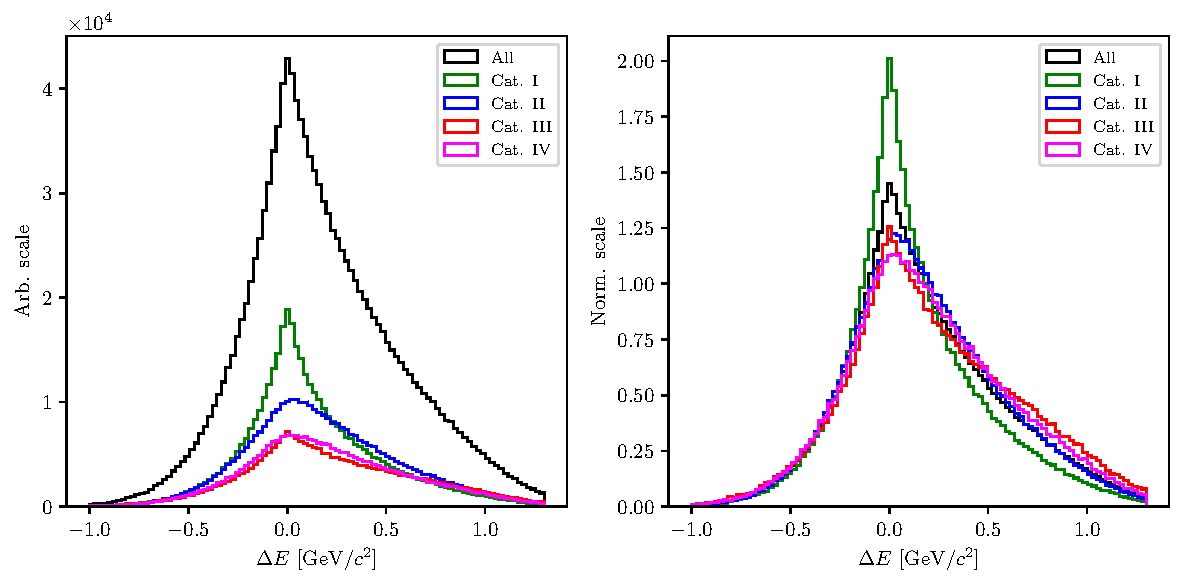
\includegraphics[width=\linewidth]{fig/sig_categ}
\caption{Categorization of signal candidates based on the charge product of both $B$ mesons in the event and the MVA output for recognizing hadronic decays of the companion $B$ meson. The plot on the left shows the distributions in an arbitrary scales, while the plot on the right shows the normalized distributions.}
\label{fig:sig_categ}
\end{figure}


\subsection{Hadronic decay MVA training}
\label{subs:HDMVA}

The Fast-BDT (FBDT) \cite{keck2017fastbdt} algorithm was used as the MVA classifier in all the following cases in this analysis. The following hyper-parameters were chosen for optimization
\begin{itemize}
\item \texttt{nTrees}: the number of trees in the FBDT forest,
\item \texttt{nLevels}: the number of levels in each FBDT tree.
\end{itemize}

Figure \ref{fig:BDT} shows a graphical interpretation of the FBDT forest with \texttt{nTrees} and \texttt{nLevels}. In all cases the hyper-parameters were optimized with a grid-search method in the hyper-parameter phase-space. 
\begin{figure}[H]
\centering
\captionsetup{width=0.8\linewidth}
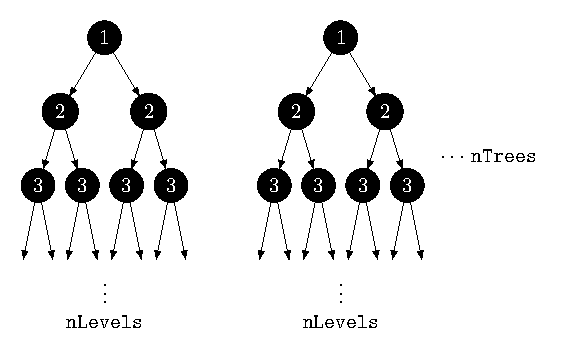
\includegraphics[scale=1]{texfig/BDT_forest}
\caption{A schematic of a BDT forest with \texttt{nTrees}, each tree having a depth of \texttt{nLevels}.}
\label{fig:BDT}
\end{figure}

In order to train an MVA classifier to recognize events with hadronically decaying $B$ mesons in the ROE side, we prepare a dataset of $2\E5$ candidates, where $50~\%$ of the candidates are signal $B$ candidates with hadronic decay of the companion $B$ meson. The remaining part of the training dataset consists of signal $B$ candidates with semi-leptonic decays of $B_{comp}$ and background $B$ candidates with hadronic and semi-leptonic decays of $B_{comp}$ in proportions $2:1:1$. 

The input variables used in this MVA are ROE specific and do not depend on the signal side. They are
\begin{itemize}
\item angle between tracks,
\item track quantities
	\begin{itemize}
	\item $P(\chi^2,DOF)$ of the tracks fit from the ROE side,
	\item $K$ and $\ell$ FlavorTagger variables,
	\item Charge of the ROE,
	\item $\cos \theta$ of the ROE momentum in the CMS frame,
	\item Number of tracks in ROE,
	\item Number of distant tracks in ROE, which don't pass requirements from Section \ref{s:ss}.
	\end{itemize}
\end{itemize}
%
The classifier output is shown in Figure \ref{fig:hdmva} (left). Candidates which populate the region with low values of the classifier output are more likely to come from semi-leptonic decays, so we want to discard those candidates. When optimizing the $\mathrm{FOM}$, we redefine the $S$ in Eq. (\ref{eq:fom}) to a correctly reconstructed signal candidate with a hadronically decayed companion $B$ meson. This $\mathrm{FOM}$ optimization, shown in Figure \ref{fig:hdmva} (right), yields the optimal cut
\begin{itemize}
\item $BDT_{had.} > 0.51.$
\end{itemize} 

\begin{figure}[H]
\centering
\captionsetup{width=0.8\linewidth}
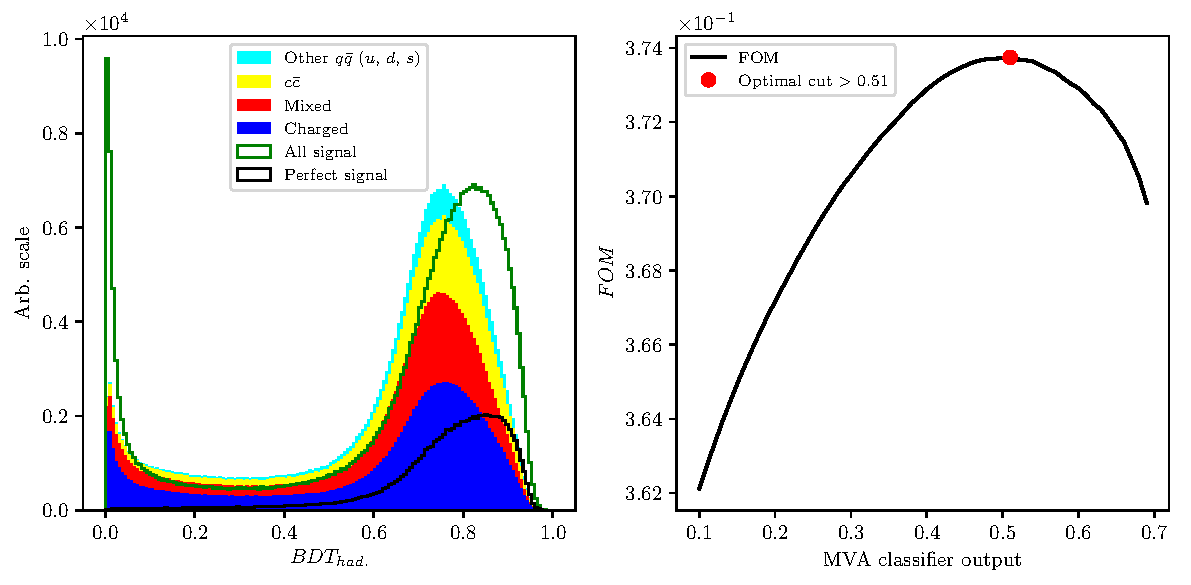
\includegraphics[width=\linewidth]{fig/hdmva_opt}
\caption{Hadronic MVA classifier output for major types of background and scaled-up signal (left), and $\mathrm{FOM}$ optimization on this cut for correctly reconstructed signal candidates with hadronically decayed companion $B$ meson (right).}
\label{fig:hdmva}
\end{figure}

More details on the hadronic MVA classifier training can be found in Appendix A.

\section{Signal region definition}

Since signal candidates are now categorized, we can define a signal region, where most of our perfectly reconstructed candidates lie. We use this region for optimizations of all cuts in the following steps of background suppression in chapter \ref{sec:background-suppression}. The 2D $\mathrm{FOM}$ optimization of the optimal $M_{BC}$ and $\Delta E$ is shown in Figure \ref{fig:sigwin}.
The signal region is defined as
\begin{itemize}
\item $M_{BC} > 5.270\e{GeV}/c^2.$,
\item $\vert \Delta E \vert < 0.166\e{Gev}$. 
\end{itemize}

\begin{figure}[H]
\centering
\captionsetup{width=0.8\linewidth}
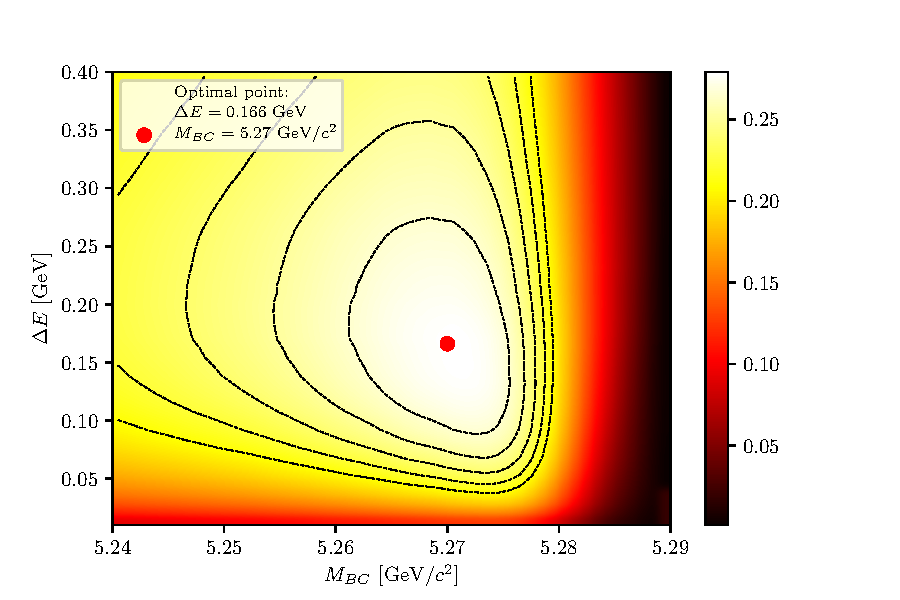
\includegraphics[width=\linewidth]{fig/sigWin}
\caption{2D $\mathrm{FOM}$ optimization of the signal region definition, where the signal in the optimization was represented by perfectly reconstructed candidates.}
\label{fig:sigwin}
\end{figure}

Lastly, we can tighten the cut on $m_{miss}^2$, which we intentionally left loose before the signal categorization. With the $\mathrm{FOM}$ optimization of perfectly reconstructed candidates inside the signal region, shown in Figure \ref{fig:missm2opt}, the optimal cut on $m_{miss}^2$ is 

\begin{itemize}
\item $\vert m_{miss}^2 \vert < 1.1\e{GeV}/c^2$.
\end{itemize}

\begin{figure}[H]
\centering
\captionsetup{width=0.8\linewidth}
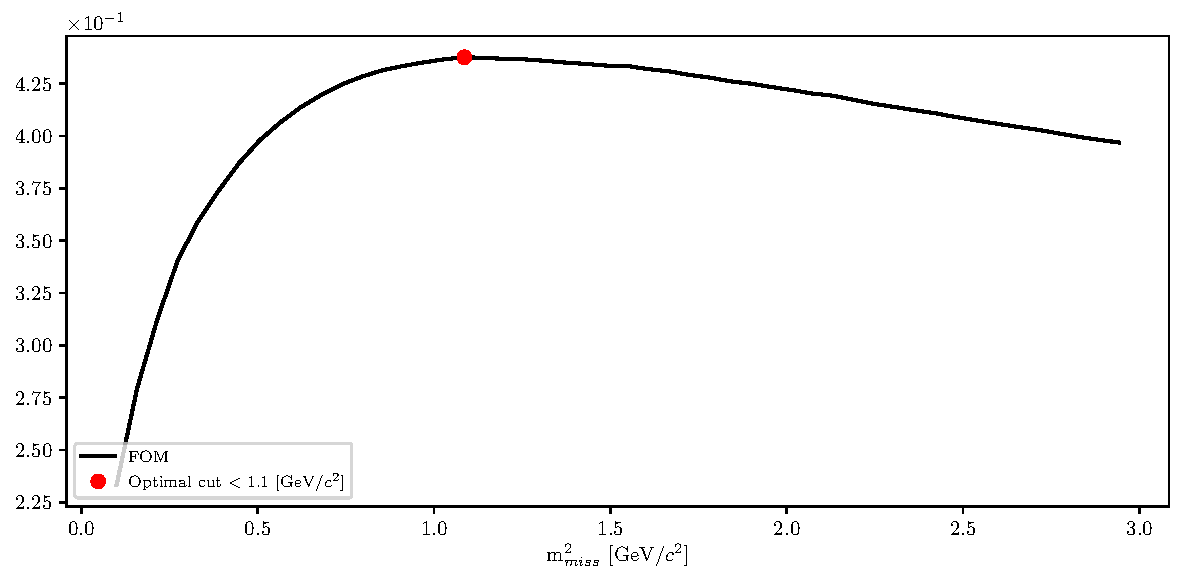
\includegraphics[width=\linewidth]{fig/missm2_opt}
\caption{$\mathrm{FOM}$ optimization of the optimal $m_{miss}^2$ cut in the signal region.}
\label{fig:missm2opt}
\end{figure}

\section{Selection summary}
\label{s:ss}
In this section one can find the summary of all selection cuts in the event reconstruction, from FSP particles up to the $B$ meson.

\begin{itemize}
\item FSP particles:
	\begin{itemize}
	\item Electrons: $\vert d_0 \vert < 0.1\e{cm},\,\vert z_0 \vert < 1,5\e{cm},\,p>0.6\e{GeV}/c,\\p_{CMS}\in[0.4,\,2.6]\e{GeV}/c,\,eID>0.9,$
    \item Muons: $\vert d_0 \vert < 0.1\e{cm},\,\vert z_0 \vert < 1,5\e{cm},\,p_{CMS}\in[0.6,\,2.6]\e{GeV}/c,\\\mu ID>0.97,$
    \item Kaons: $\vert d_0 \vert < 0.15\e{cm},\,\vert z_0 \vert < 1,5\e{cm},\,p_{CMS} < 2.5\e{GeV}/c,\\K/\pi~ID>0.6,\,K/p~ID>0.1,$
	\end{itemize}
\item $B$ meson candidates:
	\begin{itemize}
	\item Before ROE clean-up: $P(\chi^2,\,DOF) > 1\E{-3},\,\vert \cos \theta_{BY} \vert < 1,\,\vert m_{miss}^2 \vert < 7\e{GeV}/c^2,$
    \item After ROE clean-up: $\Delta E \in [-1.0,1.3]\e{GeV},\,M_{BC} \in [5.1,5.295]\e{GeV}/c^2,$
    \item After signal categorization: $q_{B^\pm}q_{B^\mp} = -1,\,BDT_{had.} > 0.51,\,\vert m_{miss}^2\vert<~1.1\e{GeV}/c^2.$
	\end{itemize}
\end{itemize}
\chapter{Rest of Event Clean-up}
\label{sec:roe}

Continuing from Section \ref{sec:loose-neutrino-reconstruction}, the description of the ROE clean-up process is described here. 

Training the MVA classifiers follows the same recipe for all the steps in this chapter. For each step, we run the $B$ meson reconstruction on Signal MC with a generic companion $B$ meson. For every correctly reconstructed signal $B$ meson candidate we save the necessary information for each MVA step (e.g. properties of ROE clusters). Only correctly reconstructed $B$ candidates are chosen here, to prevent leaks of information from the signal side to the ROE side.

More information about the MVA training, hyper-parameter optimization and feature importance for each MVA step in this chapter can be found in Appendix \ref{sec:roe-control-plots}.

\section{Clusters Clean-up}

Photons originate from the IP region, travel to the ECL part of the detector in a straight line, and produce a cluster. The direction of the photon is determined via the location of the cluster hit in the ECL and the energy of the photon is directly measured via the deposited energy. This way the four-momentum of photons is determined and used in Eq. (\ref{eq:ROEloop}).

Most of the photons in events with $B$ mesons come from processes such as $\pi^0 \to \gamma \gamma$ decays, which are interesting for physics. However, a lot of hits in the ECL are also created by photons coming from the beam-induced background or secondary interactions with the detector material, which we are usually not interested in, except in cases involving material studies. Photons of the first kind should be taken into account when calculating the missing four-momentum, while photons, which are not directly related to the collision, add extra energy and momentum to the event. In the first step of the clusters clean-up, we train an MVA which recognizes good $\pi^0$ candidates and apply this information to the daughter photons. This represents a sort of a $\pi^0$ origin probability, which peaks at or is equal to 0 for photons not coming from $\pi^0$ particles, and peaks at 1 otherwise. This information is used as an additional classifier variable in the next step of the clean-up, where we train to recognize good photons in an event.

\subsection{\texorpdfstring{$\pi^0$}{π0} MVA Training}

The training dataset of $\pi^0$ candidates contains
\begin{itemize}
	\item 183255 target candidates,
	\item 200000 background candidates,
\end{itemize}
where the definition of a target is that both photon daughters, which were used in the reconstruction of the $\pi^0$, are actual photons and real daughters of the $\pi^0$ particle. We use $\pi^0$ candidates from the converted Belle particle list and select those with the invariant mass in the range of $M \in [0.10,~0.16]\e{GeV}$. After that, we perform a mass-constrained fit on all $\pi^0$ candidates, keeping only the ones for which the fit converged. 

The input variables used in this MVA are
\begin{itemize}
	\item $p$ and $p_{CMS}$ of $\pi^0$ and $\gamma$ daughters,
	\item fit probability of the mass-constrained fit, invariant mass and significance of mass before and after the fit,
	\item angle between the photon daughters in the CMS frame,
	\item cluster quantities for each daughter photon
	\begin{itemize}
		\item $E_9/E_{25}$,
		\item theta angle,
		\item number of hit cells in the ECL,
		\item highest energy in cell,
		\item energy error,
		\item distance to closest track at ECL radius.
	\end{itemize}
\end{itemize}

The classifier output variable is shown in Figure \ref{fig:ROE_pi0}.

\begin{figure}[H]
	\centering
	\captionsetup{width=0.8\linewidth}
	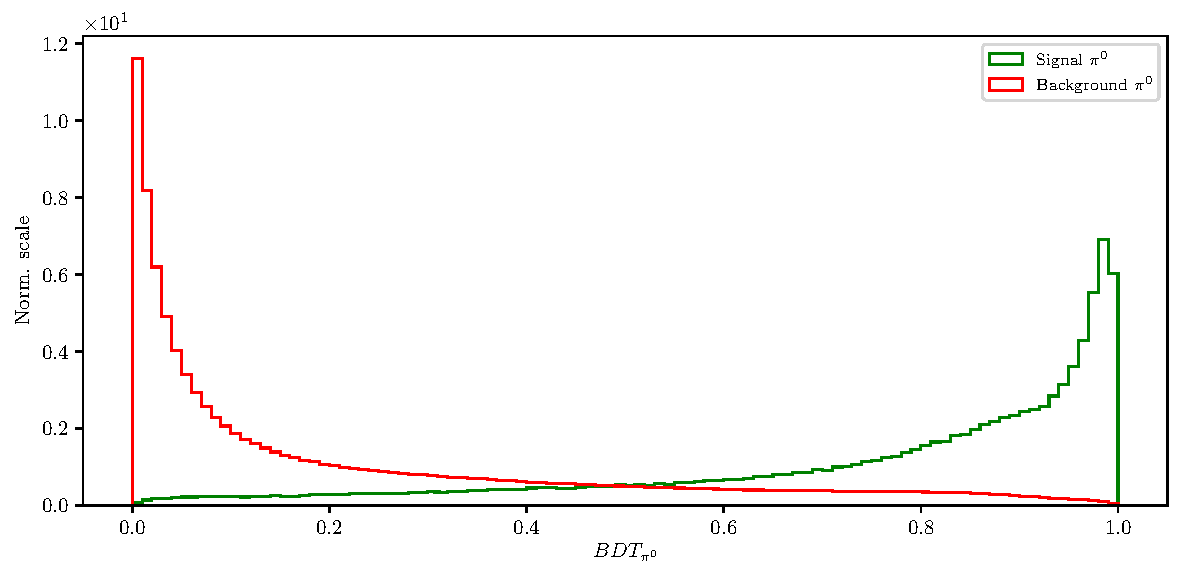
\includegraphics[width=\linewidth]{fig/ROECleanup_pi0}
	\caption{Classifier output of the $\pi^0$ training for signal and background $\pi^0$ candidates.}
	\label{fig:ROE_pi0}
\end{figure}


\subsection{\texorpdfstring{$\gamma$}{γ} MVA Training}

In this MVA training, we take the $\pi^0$ classifier output of the previous training as an input in order to train a classifier to distinguish between good and bad photons. The $\pi^0$ probability information from the previous step is applied to all photon pairs, which pass the same $\pi^0$ selection criteria, as defined in the previous step. Since it is possible to have overlapping pairs of photons, the $\pi^0$ probability is overwritten in the case of a larger value, since this points to a greater probability of a correct photon combination. On the other hand, some photon candidates fail to pass the $\pi^0$ selection. These candidates have a fixed value of $\pi^0$ probability equal to zero.

The training dataset of $\gamma$ candidates contains
\begin{itemize}
	\item 171699 target candidates,
	\item 177773 background candidates,
\end{itemize}
where the definition of a target is that the photon is an actual photon, which is related to a primary MC particle. This tags all photon particles from secondary interactions as background photons. We use the converted $\gamma$ candidates from the existing Belle particle list. 

The input variables used in this MVA are
\begin{itemize}
	\item $p$ and $p_{CMS}$ of $\gamma$ candidates,
	\item $\pi^0$ probability,
	\item cluster quantities
	\begin{itemize}
		\item $E_9/E{25}$,
		\item theta angle,
		\item number of hit cells in the ECL,
		\item highest energy in cell,
		\item energy error,
		\item distance to closest track at ECL radius.
	\end{itemize}
\end{itemize}

The classifier output variable is shown in Figure \ref{fig:ROE_gamma}.

\begin{figure}[H]
	\centering
	\captionsetup{width=0.8\linewidth}
	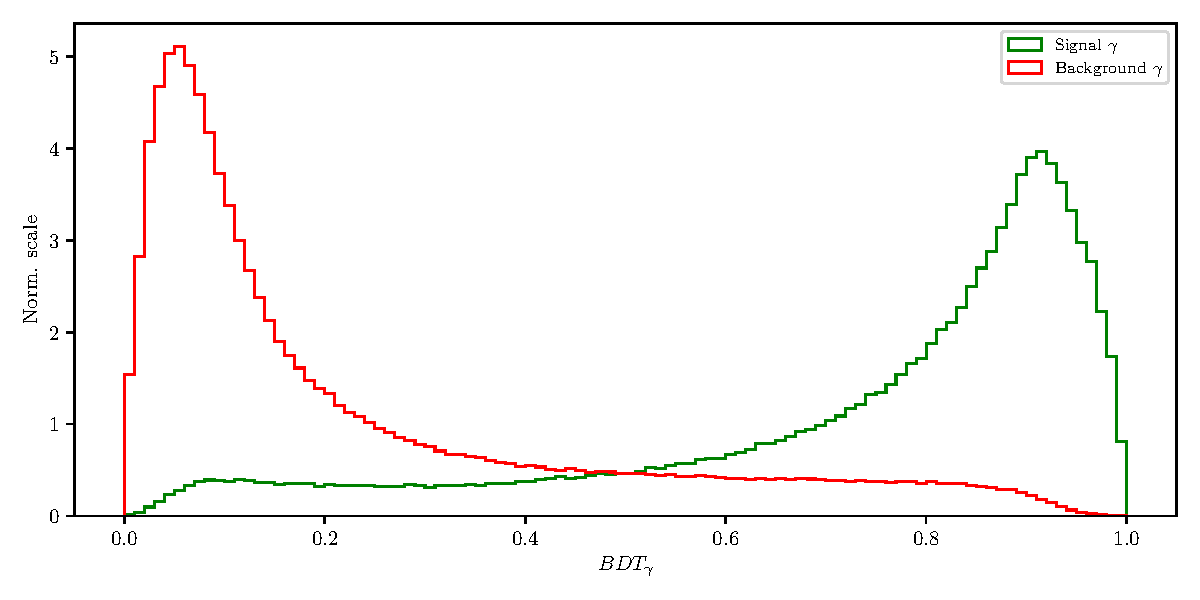
\includegraphics[width=\linewidth]{fig/ROECleanup_gamma}
	\caption{Classifier output of the $\gamma$ training for signal and background $\gamma$ candidates.}
	\label{fig:ROE_gamma}
\end{figure}

With the classifier output at hand, we apply a selection to the photon particle list. The selection optimization is shown in Figure \ref{fig:ROE_gamma_opt} (left), with the optimal selection on the $\gamma$ classifier output at
\begin{itemize}
	\item $BDT_\gamma > 0.5045$.
\end{itemize}

Figure \ref{fig:ROE_gamma_opt} (right) shows the LAB frame momentum of the photons in the logarithmic scale, before and after the selection. The signal efficiency and background rejection of this clean-up step are
\begin{itemize}
	\item Signal efficiency: $\epsilon_{SIG} = 83.2~\%$,
	\item Background rejection: $1-\epsilon_{BKG} = 81.2~\%$.
\end{itemize}

\begin{figure}[H]
	\centering
	\captionsetup{width=0.8\linewidth}
	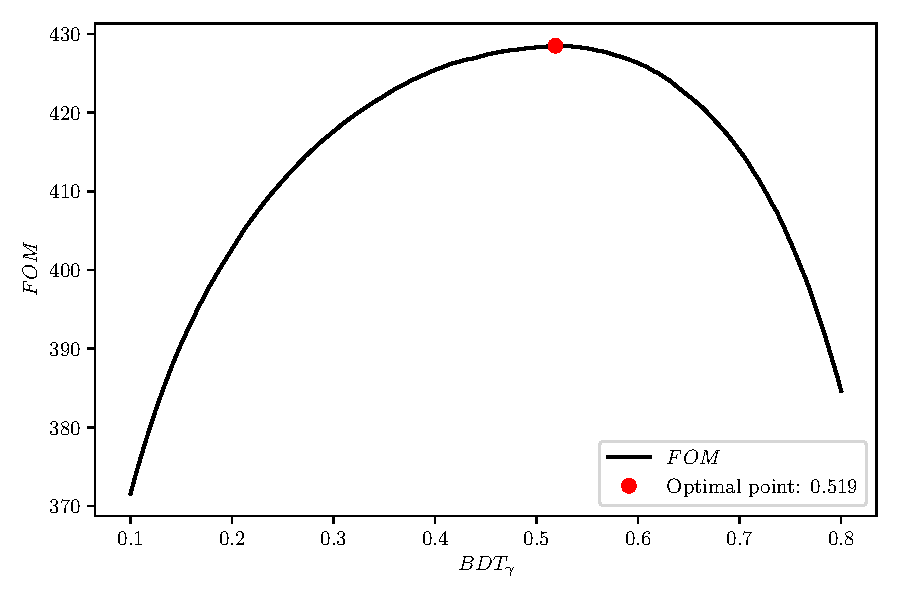
\includegraphics[width=\linewidth]{fig/ROECleanup_gamma_opt}
	\caption{The $FOM$ of the classifier output optimization (left) and  momentum magnitude in the LAB frame (right) of signal and background photon candidates before (dashed) and after (solid) the optimal selection.}
	\label{fig:ROE_gamma_opt}
\end{figure}

The event is now considered to be clean of extra clusters.

\section{Tracks Clean-up}

Charged particles leave hits in the detector, which are then grouped into tracks by advanced tracking algorithms. The track is fitted and the track momentum is determined. With the help of particle identification information (PID), we are able to make an intelligent decision about the mass hypothesis of the particle and thus reconstruct the four-momentum of the charged particle, which is then taken into account in the loop in Eq. (\ref{eq:ROEloop}).

Most of the quality (good) tracks, which come from physics event of interest, come from the IP region, where the collisions occur. Cleaning up the tracks is a more complex procedure than cleaning up the clusters. The following facts need to be taken into account
\begin{enumerate}[(a)]
	\item good tracks can also originate away from the IP region, due to decays of long-lived particles, such as $K_S^0 \to \pi^+ \pi^-$,
	\item charged particles from background sources produce extra tracks or duplicates,
	\item low momentum charged particles can curl in the magnetic field and produce multiple tracks,
	\item secondary interactions with detector material or decays of particles in flight can produce "kinks" in the flight directory, resulting in multiple track fit results per track.
\end{enumerate}

Schematics of all the cases mentioned above are shown in Figure \ref{fig:track_cleanup}.

\begin{figure}[H]
	\centering
	\subfigure[]{
		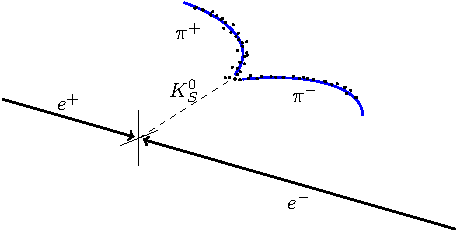
\includegraphics[width=0.49\linewidth]{texfig/V0}}%
	\subfigure[]{
		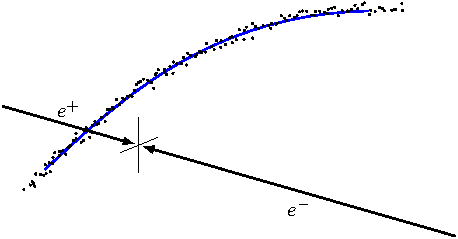
\includegraphics[width=0.49\linewidth]{texfig/background}}\\
	\subfigure[]{
		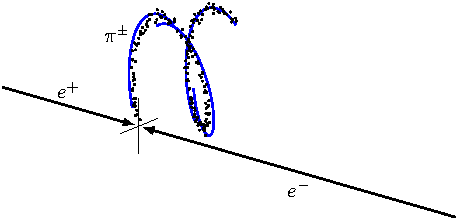
\includegraphics[width=0.49\linewidth]{texfig/curler}}%
	\subfigure[]{
		\includegraphics[width=0.49\linewidth]{texfig/decay}}%
	\captionsetup{width=.8\linewidth}
	\caption{(a) Tracks from long-lived neutral particles, which decay away from the IP region, (b) random reconstructed background tracks, (c) low-momentum particles, which curl in the magnetic field, (d) in-flight decays of particles, which produce a "kink" in the trajectory.}
	\label{fig:track_cleanup}
\end{figure}

It is obvious that tracks from the same momentum source should only be taken into account once, or, in the case of background tracks, not at all. Such tracks will, from this point on, be denoted as \textit{extra} tracks, because they add extra four-momentum to our final calculations in Eq. (\ref{eq:ROEloop}). At the same time, we have to take care that we do not identify \textit{good} tracks as \textit{extra} tracks. Both of these cases have negative impacts on the final resolution of all variables, which depend on information from ROE.

\subsection{Tracks from Long-lived Particles}

The first step in the tracks clean-up is taking care of the tracks from long-lived particles, such as $K_S^0 \to \pi^+\pi^-$, $\gamma \to e^+ e^-$ and decays of $\Lambda$ baryons. Here we only focus on $K_S^0$, since they are the most abundant. This step is necessary because of the $\pi^\pm$ particles, coming from the $K_S^0$ decays, have large impact parameters, which is usually a trait of background particles. In order to minimize confusion from the MVA point-of-view, these tracks are taken into account separately.

We use the converted $K_S^0$ candidates from the existing Belle particle list and use a pre-trained Neural Network classifier in order to select only the good $K_S^0$ candidates. Figure \ref{fig:ROE_V0} shows the distribution of the $K_S^0$ invariant mass for signal and background candidates, before and after the selection cut on the classifier output. The momentum of selected $K_S^0$ candidates is added to the ROE, while the daughter tracks are discarded from our set.

\begin{figure}[H]
	\centering
	\captionsetup{width=0.8\linewidth}
	\includegraphics[width=\linewidth]{fig/ROECleanup_V0}
	\caption{Invariant mass of the $K_S^0$ candidates before (dashed) and after (solid) the selection on the Neural Network classifier for signal (green) and background candidates (red). Signal peaks at nominal $K_S^0$ mass, while background covers a wider region.}
	\label{fig:ROE_V0}
\end{figure}

The signal efficiency and background rejection for $K_S^0$ candidates after this selection and on the full range are
\begin{itemize}
	\item Signal efficiency: $\epsilon_{SIG} = 80.7~\%$,
	\item Background rejection: $1-\epsilon_{BKG} = 99.4~\%$.
\end{itemize}

\subsection{Duplicate Tracks}
All good tracks at this point should be coming from the IP region, since we took care of all the good tracks from long-lived particle decays, therefore we apply a selection on impact parameters for all the remaining tracks
\begin{itemize}
	\item $\vert d_0 \vert < 10\e{cm}$ and $\vert z_0 \vert < 20\e{cm}$
\end{itemize} 

and proceed with the clean-up of track duplicates.

\subsubsection{Defining a duplicate track pair}

In this step, we wish to find a handle on secondary tracks from low momentum curlers and decays in flight. The main property for these cases is that the 3D opening angle between such two tracks is very close to $0^\circ$ or $180^\circ$, since the tracks deviate only slightly from the initial direction, but can also be reconstructed in the opposite way. Figure \ref{fig:ROE_dupAngleInit} shows the distribution of the angle between two tracks in a single pair for random track pairs and duplicate track pairs, where the latter were reconstructed as two same-sign or opposite-sign tracks.

\begin{figure}[H]
	\centering
	\captionsetup{width=0.8\linewidth}
	\includegraphics[width=\linewidth]{fig/ROECleanup_dup_angle_initial}
	\caption{Distribution of the angle between two tracks in a single pair for random track pairs (green) and duplicate track pairs, where the latter were reconstructed as two same-sign (blue) or opposite-sign tracks (red).}
	\label{fig:ROE_dupAngleInit}
\end{figure}

If the particle decayed mid-flight or produced multiple tracks due to being a low-momentum curler, then, as the name suggests, these particles most likely a had low momentum in the transverse direction, $p_T$. Since both tracks originate from the same initial particle, the momentum difference should also peak at small values. Figure \ref{fig:ROE_dupPt} shows the momentum and momentum difference of tracks which belong to a random or a duplicate track pair.

\begin{figure}[H]
	\centering
	\captionsetup{width=0.8\linewidth}
	\includegraphics[width=\linewidth]{fig/ROECleanup_dup_pt}
	\caption{Distribution of transverse momentum $p_T$ (left) and transverse momentum difference $\Delta p_T$ (right) for all tracks coming from random (green) or duplicate track pairs (red). The plot on the right already includes the selection on $p_T$ from the plot on the left.}
	\label{fig:ROE_dupPt}
\end{figure}

We impose a selection of
\begin{itemize}
	\item $p_T < 0.5\e{GeV}/c$,
	\item $\vert \Delta p_T \vert < 0.1\e{GeV}/c$,
\end{itemize}

in order to minimize the number of random track pairs, while retaining a high percentage of duplicate track pairs. After applying the selection criteria defined in this chapter, the final distribution of the angle between two tracks is shown in Figure \ref{fig:ROE_dupAngleFinal}.

\begin{figure}[H]
	\centering
	\captionsetup{width=0.8\linewidth}
	\includegraphics[width=\linewidth]{fig/ROECleanup_dup_angle_final}
	\caption{Distribution of the angle between two tracks in a single pair after applying the selection defined in this section. The distributions are shown for random track pairs (green) and duplicate track pairs, where the latter were reconstructed as two same-sign (blue) or opposite-sign tracks (red).}
	\label{fig:ROE_dupAngleFinal}
\end{figure}

\subsubsection{Training the duplicate track pair MVA}
\label{ss:trackMVA}

This final sample of track pairs is used in the MVA training to recognize duplicate track pairs. The training dataset contains
\begin{itemize}
	\item 113707 target candidates,
	\item 190314 background candidates,
\end{itemize}
where the definition of a target is that the track pair is a duplicate track pair. 

The input variables used in this MVA are
\begin{itemize}
	\item angle between tracks,
	\item track quantities
	\begin{itemize}
		\item impact parameters $d_0$ and $z_0$,
		\item transverse momentum $p_T$,
		\item helix parameters and helix parameter errors of the track,
		\item track fit $p$-value,
		\item number of hits in the SVD and CDC detectors
	\end{itemize}
\end{itemize}

The classifier is able to distinguish between random and duplicate track pairs in a very efficient manner, as shown in Figure \ref{fig:ROE_dupBDT}.

\begin{figure}[H]
	\centering
	\captionsetup{width=0.8\linewidth}
	\includegraphics[width=\linewidth]{fig/ROECleanup_dup}
	\caption{Classifier output of the track pair training for random track pairs and duplicate track pairs.}
	\label{fig:ROE_dupBDT}
\end{figure}

The $FOM$ function for optimal selection is shown in Figure \ref{fig:ROE_dupOpt} (left), along with the angle between the two tracks before and after the optimal selection (right). The optimal duplicate track selection is
\begin{itemize}
	\item $BDT_{duplicate} > 0.9985.$
\end{itemize}

The signal efficiency and background rejection for duplicate pair candidates after this selection is
\begin{itemize}
	\item Signal efficiency: $\epsilon_{SIG} = 87.2~\%$,
	\item Background rejection: $1-\epsilon_{BKG} = 98.8~\%$,
\end{itemize}
where signal and background represent duplicate and random track pairs, respectively.


\begin{figure}[H]
	\centering
	\captionsetup{width=0.8\linewidth}
	\includegraphics[width=\linewidth]{fig/ROECleanup_dup_opt}
	\caption{The optimization of the $FOM$ function for the cut on classifier output (left) and distribution of the angle between two tracks in a single pair before (dashed) and after (solid) applying the optimal cut on the output classifier for random and duplicate track pairs (right).}
	\label{fig:ROE_dupOpt}
\end{figure}

\subsubsection{Defining duplicate tracks}

What remains now is to decide which track from the duplicate track pair to keep and which to discard. For this purpose, we apply duplicate pair-level information to each track in the pair in the form of
\begin{equation}
\Delta f = f_{this} - f_{other},
\end{equation}

where $f$ is an arbitrary variable from the list of track quantities in Section \ref{ss:trackMVA}. From the point-of-view of \textit{this} track, a track is more $duplicate$-like if the following is true
\begin{itemize}
	\item $\Delta d_0,\,\Delta z_0 > 0$ (\textit{this} track further away from the IP region),
	\item $\Delta p_T,\,\Delta p_Z < 0$ (\textit{this} track has lower momentum),
	\item $\Delta N_{SVD},\,\Delta N_{CDC} < 0$ (\textit{this} track has less hits in the SVD and CDC),
\end{itemize}

Additionally we define an MC truth variable 
\begin{equation}
\label{eq:chi2}
\Delta \chi^2 = \chi^2_{this} - \chi^2_{other},\quad\chi^2 = \sum_{i=x,y,z}\frac{\left(p_i - p_i^{MC}\right)^2}{\sigma(p_i)^2},
\end{equation}
where we compare all components of track momentum to the true values. If the condition $\Delta \chi^2 > 0$ is satisfied, then \textit{this} track is probably a duplicate track and should be discarded.

However, it turns out that solving this problem is not as simple as discarding one track and keeping the other one. An additional complication here is that we can have more than one extra track from the same initial particle, which leads to track pairs, where both tracks are track duplicates. For example, if we have the following case
\begin{align*}
t_1&: \mathrm{good~track},\\
t_2&: \mathrm{extra~track},\\
t_3&: \mathrm{extra~track},\\
\mathrm{pair}_1&:\left(t_1,t_2\right),\\
\mathrm{pair}_2&:\left(t_1,t_3\right),\\
\mathrm{pair}_3&:\left(t_2,t_3\right),
\end{align*}
where $t_1$ is the original track and $t_2$ and $t_3$ are extra tracks, with $t_3$ being even more duplicate-like with respect to $t_2$. Here tracks $t_2$ and $t_3$ should be discarded while $t_1$ should be kept. We can achieve this, if we overwrite existing pair-level information in the tracks for cases, where the variable difference $\Delta f$ is more duplicate-like. If we follow the same example, we could fill information about the property $f$ in six different orders. 
\begin{align*}
1.&~\left(t_1,t_2*\right)\quad \to \quad \left(t_1,t_3*\right)\quad \to \quad \left(t_2*,t_3*\right),\\ 
2.&~\left(t_1,t_2*\right)\quad \to \quad \left(t_2*,t_3*\right)\quad \to \quad \left(t_1,t_3*\right),\\ 
3.&~\left(t_1,t_3*\right)\quad \to \quad \left(t_2,t_3*\right)\quad \to \quad \left(t_1,t_2*\right),\\
4.&~\left(t_1,t_3*\right)\quad \to \quad \left(t_1,t_2*\right)\quad \to \quad \left(t_2*,t_3*\right),\\
5.&~\left(t_2,t_3*\right)\quad \to \quad \left(t_1,t_3*\right)\quad \to \quad \left(t_1,t_2*\right),\\
6.&~\left(t_2,t_3*\right)\quad \to \quad \left(t_1,t_2*\right)\quad \to \quad \left(t_1,t_3*\right),
\end{align*}

where the "*" symbol denotes when a track is recognized as a duplicate track with respect to the other track. If you are a part of my defense committee and actually read this before my thesis defense, let me know, I owe you a bottle of whiskey. We see that no matter the order, both $t_2$ and $t_3$ get recognized as duplicate tracks correctly.

\subsubsection{Training the duplicate track MVA}
The training procedure is similar as before. The sample of tracks from duplicate track pairs is now used in the MVA training to distinguish duplicate tracks from good tracks. The training dataset contains
\begin{itemize}
	\item 84339 target candidates,
	\item 68280 background candidates,
\end{itemize}
where the definition of a target is that the track is a duplicate track, based on the $\Delta \chi^2 > 0$ condition.

The input variables used in this MVA are
\begin{itemize}
	\item theta angle of the track momentum,
	\item track quantities
	\begin{itemize}
		\item impact parameters $d_0$ and $z_0$ and their errors,
		\item CMS frame momentum $p_{CMS}$ and momentum components $p_T$ and $p_z$ 
		\item number of hits in the SVD and CDC detectors
		\item track fit $p$-value,
	\end{itemize}
	\item pair-level information
	\begin{itemize}
		\item $\Delta d_0$, $\Delta z_0$, $\Delta N_{CDC}$, $\Delta N_{SVD}$, $\Delta p_T$, $\Delta p_z$, $\Delta p$-value.  
	\end{itemize}
\end{itemize}

The output classifier information is added to the tracks, where now each track has a certain probability of being a duplicate track. We then compare these values between both tracks in each track pair as
\begin{equation}
\Delta BDT_{final} = BDT_{final}^{this} - BDT_{final}^{other},
\end{equation}
which is again applied to all track pairs and overwritten for tracks which are more duplicate-like. The classifier output and the classifier output difference for each track are shown in Figure \ref{fig:ROE_curl}. 

\begin{figure}[H]
	\centering
	\captionsetup{width=0.8\linewidth}
	\includegraphics[width=\linewidth]{fig/ROECleanup_curl}
	\caption{Classifier output of the MVA training for curling track recognition (left) and difference of the classifier output, calculated for each track in a track pair (right).}
	\label{fig:ROE_curl}
\end{figure}

Finally, we select all duplicate tracks, which survive the selection 
\begin{equation}
\Delta BDT_{final} > 0,
\end{equation}

and discard them from our ROE. We can check the performance of our duplicate track classifier by applying the procedure to a validation sample of duplicate track pairs and compare the predicted result with the truth, based on Eq. (\ref{eq:chi2}). Table \ref{tab:rat} shows the performance of the duplicate track recognition in the form of percentages of correctly and incorrectly identified duplicate and original tracks. The model seems to perform well and the event is now considered to be clean of duplicate tracks.

\begin{table}[H]
	\centering
	\begin{tabular}{c|c|c}
		& Predicted duplicate track & Predicted good track \\
		\toprule
		Duplicate track & $83.07~\%$  & $22.62~\%$  \\
		Good track & $16.93~\%$ & $77.38\%$ \\
		\bottomrule
	\end{tabular}
	\captionsetup{width=.8\linewidth}
	\caption{Ratios of correctly classified and misclassified tracks.}
	\label{tab:rat}
\end{table}

\section{Belle Clean-up}

For comparison, we define the Belle clean-up, used standardly at Belle, which is much simpler and relies only on a set of basic selection criteria for neutral and charged particles. This clean-up procedure is not applied in addition to our ROE clean-up, but separately, only for comparison. 

In the case of photons, only a selection on the photon energy is applied, depending on the region where the photon hit the relevant part of the detector. The photon selection is summarized in Table \ref{tab:bellegamma}.

\begin{table}[H]
	\centering
	\begin{tabular}{c|c|c|c}
		& $17^\circ < \theta < 32^\circ$ & $32^\circ < \theta < 130^\circ$ & $130^\circ < \theta < 150^\circ$ \\
		\toprule
		$E_\gamma$ & $> 100\e{MeV}$  & $> 50\e{MeV}$ & $> 150\e{MeV}$  \\
		\bottomrule
	\end{tabular}
	\captionsetup{width=.8\linewidth}
	\caption{Photon selection for the Belle clean-up procedure. Different selection criteria are applied on photons in different parts of the detector.}
	\label{tab:bellegamma}
\end{table}

In case of tracks, pairs are selected which satisfy the following criteria:
\begin{itemize}
	\item $p_T < 275\e{MeV}/c$,
	\item $\Delta p = \vert \vec{p}_1 - \vec{p}_2\vert  < 100\e{MeV}/c$,
	\item $\cos \theta (\vec{p}_1,\vec{p}_2) < 15^\circ$ for same sign,
	\item $\cos\theta(\vec{p}_1,\vec{p}_2) > 165^\circ$ for opposite sign.
\end{itemize}

Of the two tracks, the one with a larger value of formula in Eq. \ref{eq:belleformula} is discarded. The remaining tracks in the event then need to satisfy the conditions described in Table \ref{tab:belletrack}.
\begin{equation}
\label{eq:belleformula}
\left(\gamma\vert d_0 \vert \right)^2 + \vert z_0 \vert^2, \quad \gamma = 5.
\end{equation}

\begin{table}[H]
	\centering
	\begin{tabular}{c|c|c|c}
		& $p_T < 250\e{MeV}/c$ & $250\e{MeV}/c < p_T < 500\e{MeV}/c$ & $p_T > 500\e{MeV}/c$ \\
		\toprule
		$\vert d_0 \vert$ & $< 20\e{cm}$  & $< 15\e{cm}$ & $< 10\e{cm}$  \\
		$\vert z_0 \vert$ & $< 100\e{cm}$  & $< 50\e{cm}$ & $< 20\e{cm}$  \\
		\bottomrule
		
	\end{tabular}
	\captionsetup{width=.8\linewidth}
	\caption{Track selection for the Belle clean-up procedure. Different selection criteria are applied to tracks in different $p_T$ regions.}
	\label{tab:belletrack}
\end{table}

\section{Clean-up Results}

In this section, the results of the ROE clean-up are shown. It is obvious that cleaning up the event affects the shape of various distributions, especially \vars, which we are most interested in. Since the reconstruction procedure includes applying selection criteria on the cleaned-up variables, the clean-up also affects the efficiency of the reconstructed sample, not only the resolution. 

We compare the clean-up setup, defined in this analysis, to the standard clean-up used by Belle, and to a default case, where no clean-up was applied at all. We apply the clean-up procedure to our signal MC sample with all the applied selection criteria, defined in Section \ref{s:ss}, except for the signal categorization. Figure \ref{fig:roeopt} (left) shows signal candidate distributions of \vars~for various clean-up setups. Focusing on the ROE clean-up, we see an improvement in resolution in both observed variables and an overall decrease in efficiency. The efficiency decrease is expected since the cleaned-up variables are able to better isolate the perfectly reconstructed candidates and discard the non-perfect candidates. In fact, the efficiency of the perfectly reconstructed candidates increases after the ROE clean-up, as shown in Figure \ref{fig:roeopt} (right). The signal MC sample in case of the Belle clean-up also shows a slight improvement in the resolution after the procedure, but looking at the perfectly reconstructed candidates, we see that this clean-up procedure is not optimal. Table \ref{tab:roeeff} shows ratios of efficiencies and $FWHM$'s of the clean-up procedures for the perfect signal with respect to the default case, based on the $\Delta E$ distribution. While both, the Belle and ROE clean-up, improve the resolution, ROE clean-up performs significantly better and also increases the amount of the perfectly reconstructed candidates in the final sample.

\begin{figure}[H]
	\centering
	\captionsetup{width=0.8\linewidth}
	\includegraphics[width=\linewidth]{fig/roe_opt}
	\caption{\vars~distributions for various types of clean-up procedures. The figures on the left are shown for the full signal sample after the stated selection criteria, while the figures on the right are shown for the perfectly reconstructed signal candidates. For ROE clean-up, the procedure seems to improve resolution as well as increase the amount of perfectly reconstructed candidates, relative to the default case.}
	\label{fig:roeopt}
\end{figure}

\begin{table}[H]
	\centering
	\begin{tabular}{c|c|c}
		& Efficiency ratio & FWHM ratio \\
		\toprule
		Belle clean-up & $28.5~\%$  & $75.0~\%$  \\
		ROE clean-up & $140.1~\%$ & $35.0~\%$ \\
		\bottomrule
	\end{tabular}
	\captionsetup{width=.8\linewidth}
	\caption{Comparison of efficiencies and $FWHM$'s of ROE and Belle clean-up setups with respect to the default case (no clean-up) for the perfect signal.}
	\label{tab:roeeff}
\end{table}

Another variable which heavily depends on the clean-up is the charge product of the signal and companion $B$ meson candidate, already defined in Eq. (\ref{eq:chargeprod}), shown in Figure \ref{fig:roe_chargeproduct} for various clean-up procedures. The figure shows an improved resolution of the distribution of the charged product, which means that candidates migrate to the correct value of the charge product after the clean-up. Looking at the perfectly reconstructed candidates, we again see the increase in the bin corresponding to the correct charge product. As a cross-check, we can also look at \vars~variables for each value of the charge product. These plots are shown for the full signal MC sample in Figure \ref{fig:roe_split} and they show a clear resolution improvement for the correct value of the charge product in the case of the ROE clean-up. For other values of the charge product there also seems to be a small improvement for both cases of clean-up, but it is negligible compared to the plots for the optimal charge product value. This supports our choice of signal categorization, defined in Section \ref{sec:event-categorization}, where we select only candidates with the correct value of the charge product.

\begin{figure}[H]
	\centering
	\captionsetup{width=0.8\linewidth}
	\includegraphics[width=\linewidth]{fig/roe_chargeprod}
	\caption{Distribution of the charge product of both $B$ mesons for various types of clean-up procedures, shown on the full signal MC (left) and for the perfectly reconstructed signal candidates (right). For ROE clean-up, the procedure seems to increase the number of perfectly reconstructed candidates.}
	\label{fig:roe_chargeproduct}
\end{figure}

\begin{figure}[H]
	\centering
	\captionsetup{width=0.8\linewidth}
	\includegraphics[width=\linewidth]{fig/roe_split}
	\caption{Distributions of $\Delta E$ (top) and $M_{BC}$ (bottom) for various types of clean-up procedures, split by specific values of the charge product, shown for the full signal MC. There is a significant improvement in resolution after ROE-cleanup, for the case of the correct value of the charge product.}
	\label{fig:roe_split}
\end{figure}

\section{ROE Clean-up Validation}

The ROE clean-up seems to perform well on signal MC, based on the results in the previous section. However, it is necessary to make sure that this procedure performs as well on other simulated and measured data, which is done in this section. The clean-up procedure is validated on the control sample, $$B^+ \to \bar D {}^0 \ell^+ \nu,\quad D^0 \to K^+K^-,$$
which was already defined in Section \ref{sec:control-decay}. The control candidates are reconstructed in the same manner as the signal candidates. In addition to the same selection criteria applied, as in the previous section, we also apply a selection to make the control sample more significant. We keep only the candidates passing the following selection cut on the invariant mass of the two kaons
\begin{equation}
1.849\e{GeV}/c^2 < m_{KK} < 1.879\e{GeV}/c^2
\end{equation}
as shown in Figure \ref{fig:roe_mKK}. Further detail about this cut can be found in Section \ref{sec:res_bkg}.
\begin{figure}[H]
	\centering
	\captionsetup{width=0.8\linewidth}
	\includegraphics[width=\linewidth]{fig/roe_mKK_cut}
	\caption{Normalized distributions of $m_{KK}$ for the full MC dataset. The red lines represent the edges of the selection in the $m_{KK}$ distribution where the control sample is enhanced. The $m_{KK}$ distribution drops quickly for the case of the control decay, while staying uniform for other contributions.}
	\label{fig:roe_mKK}
\end{figure}

With the control sample selection determined, we now run the reconstruction with and without the ROE clean-up procedure on all available MC and data.

The effects of the ROE clean-up are shown in Figure \ref{fig:roe_val}, where we overlay the data points to a stacked histogram of MC contributions for \vars. We see that the data and MC agree well. A slight systematic trend can be seen in the $\Delta E$ variable, which is addressed in Section \ref{sec:smearing-and-offset-parameters}. The control sample resolution seems very poor in the case without the clean-up, but it improves significantly if the clean-up procedure is applied, as expected. The simulated background also seems to gain an improvement in the resolution, but this is likely due to the background consisting of similar candidates as the control sample. This means that the clean-up performs as expected due to the nature of the decays and does not arbitrarily shape the background to be more signal like. Additionally, it should be pointed out that, after the clean-up, the simulated background resolution is worse compared to the control decay resolution, while this is not the case if the clean-up procedure is not performed.
\begin{figure}[H]
	\centering
	\captionsetup{width=0.8\linewidth}
	\includegraphics[width=\linewidth]{fig/roe_val}
	\caption{Distributions of $\Delta E$ (top) and $M_{BC}$ bottom for the case without (left) and with ROE clean-up (right). The resolution of the control sample is improved and the MC and data agree well in all aspects. While the simulated background resolution is also improved, it is worse compared to the resolution of the control sample.}
	\label{fig:roe_val}
\end{figure}

To perform the clean-up validation in greater detail, we also compare the data and MC agreement in bins of the charge product of the two $B$ mesons. Figure \ref{fig:roe_val_split} shows the cleaned-up versions of \vars~for each charge product bin in the same manner as shown in the previous section. We see that the MC and data agreement persists in all cases. 
\begin{figure}[H]
	\centering
	\captionsetup{width=0.8\linewidth}
	\includegraphics[width=\linewidth]{fig/roe_val_split}
	\caption{Distributions of $\Delta E$ (top) and $M_{BC}$ (bottom) split in bins of the charge product of the two $B$ mesons.}
	\label{fig:roe_val_split}
\end{figure}

The ROE clean-up procedure seems to perform well. It significantly improves the resolution of the control and, therefore, signal candidates and increases the amount of perfectly reconstructed events. The clean-up procedure was also applied to data and no disagreement with respect to the simulated MC samples was found. This means that the procedure does not differ between MC and data and does not perform on them differently. The procedure was therefore validated in great detail and is suitable to be used in this analysis.
\chapter{Background suppression}\label{sec:background-suppression}

This chapter shows the procedure in suppressing various kinds of background by applying cuts on MVA classifier outputs. 

\section{Resonant background}

In this analysis we study decays with kaons in the final state. This means that standard procedures in $b \to u$ analyses in order to suppress $b \to c$ backgrounds, such as $K$-veto, are not possible. As a consequence, our final sample consists of combinations of $K$ pairs coming also from $b \to c$  sources, such as $D^0 \to K^+ K^-$. Such candidates usually have resonance-like properties in the two-kaon invariant mass spectrum. Figure \ref{fig:res_bkg} shows this invariant mass spectrum of two kaons, $m_{KK}$, where obvious resonant structures are present from sources like
\begin{itemize}
\item $\phi \to K^+K^-$ (sharp resonance at $\sim1.019\e{GeV}/c^2$),
\item $D^0 \to K^+K^-$ (sharp peak at $\sim 1.864\e{GeV}/c^2$),
\item $D^0 \to K^+ \pi^-$ (wide, shifted peak, due to kaon miss-identification).
\end{itemize}

In order to suppress these resonant backgrounds while studying the signal or control decay, we impose a set of the following cuts
\begin{itemize}
\item Signal cut: $\vert m_{KK} - m_{\phi} \vert > \Delta_\phi$, $\vert m_{KK} - m_{D^0} \vert > \Delta_{D^0}$, $\vert m_{K\pi} - m_{D^0} \vert > \Delta_{D^0}$,
\item Control cut: $\vert m_{KK} - m_{D^0} \vert \leq \Delta_{D^0}$, $\vert m_{K\pi} - m_{D^0} \vert > \Delta_{D^0}$,
\end{itemize}

where $m_\phi \approx 1.019\e{GeV}/c^2$ and $m_{D^0} \approx 1.864\e{GeV}/c^2$ are nominal masses of the $\phi$ and $D^0$ mesons, and $\Delta_\phi \approx 8\E{-3}\e{GeV}/c^2$ and $\Delta_{D^0} \approx 1.2\E{-2}\e{GeV}/c^2$ are symmetric cut widths around the nominal mass values for the $\phi$ and $D^0$ mesons, respectively.

By imposing the signal cut, as defined above, on the full sample at this stage, we are able to suppress $94.6~\%$ and $86.4~\%$ of the control candidates and candidates with the $\phi$ intermediate state, respectively, while retaining $95.9~\%$ of signal candidates. On the other hand, by imposing the control cut, we suppress $98.4~\%$ and $100.0~\%$ of the signal candidates and candidates with the $\phi$ intermediate state, respectively, while retaining $98.4~\%$ of the control candidates. We see that both cuts are very efficient in isolating the desired subsamples, which is very useful for further studies.

\begin{figure}[H]
\centering
\captionsetup{width=0.8\linewidth}
\includegraphics[width=\linewidth]{fig/res_bkg}
\caption{Invariant mass of two correctly reconstructed kaons (left) and invariant mass of two kaons, where one was miss-identified as a pion (right).}
\label{fig:res_bkg}
\end{figure}


\section{Continuum suppression}

Continuum background are physics processes where continuum states are produced in electron and positron collisions $$e^+ e^- \to q \bar q,$$ 
where $q = u,~d,~s$ or $c$, and are a sizable contribution to $B \bar B$ events. Additionally to kinematic constraints to separate $e^+ e^- \to \Upsilon(4S) \to B \bar B$ decays from $e^+ e^- \to q \bar q$, properties of the "event shape" are also often used, because phase-space distributions of decayed particles differ for these two processes. Continuum background events are generated in a back-to-back way in the CMS frame, so hadrons produced in the quark fragmentation possess only a small transverse momentum compared to the initial momentum magnitude. This leads to a spatially confined, jet-like structure. On the other hand $B$ mesons from $B \bar B$ events are produced almost at rest in the CMS frame. Their decay products from an isotropic distribution in the detector, which yields a spherical event shape.

\subsection{Characteristic variables}
\label{ss:charvar}
Information on the phase-space distribution of decay particles is obtained in a number of different ways. In this subsection different characteristic variables are presented which are used in the MVA training. They all focus on kinematic and shape differences between the two processes, which we want to discriminate. 

%\subsubsection{$B$ meson direction}
%Two $B$ mesons, coming from a spin-1 $\Upsilon(4S)$ meson, both have 0 spin, which results in a $\sin^2\theta_B$ angular distribution of the $B$ meson direction with respect to the beam axis. On the other hand, $q \bar q$ final states are represented by two half-spin fermions, which results in two jets, following a $1+\cos^2\theta_B$ distribution. The variable $\vert \cos \theta_B \vert$ allows one to discriminate between $B$ candidates from $B \bar B$ decays and continuum background. Figure X shows the distribution of $\vert \cos \theta_B \vert$ for different $B$ meson candidates.

\subsubsection{Thrust and related variables}
It is possible to define a thrust axis $\mathbf{T}$ for a collection of $N$ momenta $p_i$ as a unit vector along which their total projection is maximal. Thrust axis $\mathbf T$ can be obtained by maximizing the expression
\begin{equation}
\mathbf{T} = \frac{\sum_{i}\vert \mathbf{T} \cdot \mathbf{p}_i\vert}{\sum_{i}\vert \mathbf{p}_i\vert}.
\end{equation}
In this case, a related variable is $\vert \cos\theta_T\vert$, where $\theta_T$ is the angle between the thrust axis of the momenta from $B$ meson decay particles, and the thrust axis of all particles in the ROE. Since both $B$ mesons in $B \bar B$ events are produced at rest, their decay particles, and consequentially their thrust axes, are uniformly distributed in the range $[0,~1]$. On the other hand, decay particles from continuum events follow the direction of the jets in the event. As a consequence, the thrusts of both the $B$ meson and the ROE are strongly directional and collimated, which results in a large peak at $\vert \cos\theta_T\vert \approx 1$. Additionally, one can also use the variable $\vert \cos\theta_{TB}\vert $, which is the thrust axis between the $B$ candidate and the beam axis. For $B$ candidates from $B \bar B$, this distributions is again uniformly distributed, while for candidates from continuum events this distribution follows the distribution of the jets with the function $1+\cos^2\theta_{T,B}$. Figure \ref{fig:cosplots} shows the distributions of $\vert \cos\theta_T\vert$ (left) and $\vert \cos\theta_{T,B}\vert$ (right) for different $B$ meson candidates.

\begin{figure}[H]
\centering
\captionsetup{width=0.8\linewidth}
\includegraphics[width=\linewidth]{fig/cs_cosplots}
\caption{Distributions of $\vert \cos\theta_T\vert$ (left) and $\vert \cos\theta_{T,B}\vert$ (right) for different $B$ meson candidates.}
\label{fig:cosplots}
\end{figure}

\subsubsection{CLEO cones}
CLEO cones have been introduced by the CLEO collaboration \cite{asner1996search} and are an additional specific tool to provide optimal background discrimination. They are nine variables corresponding to the momentum flow around the thrust axis of the $B$ meson candidate, binned in nine cones of $10^\circ$ around the thrust axis, as illustrated in Figure \ref{fig:ccones}. 

\begin{figure}[H]
\centering
\captionsetup{width=0.8\linewidth}
\includegraphics[scale=1]{texfig/CCones}
\caption{Concept of CLEO cones. $\mathbf{T}$ denotes the thrust axis of the $B$ meson candidates in the event. Each variable corresponds to a momentum flow around the thrust axis in steps of $10^\circ$.}
\label{fig:ccones}
\end{figure}

\subsubsection{KSFW moments}
Fox-Wolfram moments are another useful parametrization of phase-space distribution of energy flow and momentum in an event. For a collection of $N$ momenta $p_i$, the $k$-th order normalized Fox-Wolfram moment $R_k$ is defined as
\begin{equation}
R_k = \frac{H_k}{H_0} = \frac{1}{H_0} \sum_{i,j} \vert p_i \vert \vert p_j \vert P_k(\cos \theta_{ij}),
\end{equation}
where $\theta_{ij}$ is the angle between $p_i$ and $p_j$, and $P_k$ is the $k$-th order Legendre polynomial. For events with two strongly collimated jets, $R_k$ takes values close to 0 (1) for odd (even) values of $k$, so these moments provide a convenient discrimination between $B \bar B$ and continuum events.

Belle developed a refined generation of Fox-Wolfram moments, called Kakuno-Super-Fox-Wolfram (KSFW) moments to further suppress the continuum background. There are $17$  different KSFW moments which are grouped into $R^{so}_k$, $R^{oo}_k$ and $R^{ss}_k$ \cite{bevan2014physics}. The latter ones are excluded due to correlations with $B$ meson specific variables.

\subsection{MVA training}
\label{ss:qqmva}
Most of the characteristic variables, described in subsection \ref{ss:charvar}, were taken together in order to train a single MVA classifier for continuum suppression. All characteristic variables were checked for possible $q^2$ correlation. Variables with significant correlation or complex shapes in the 2D plot were discarded from the training set, since they would have introduced unwanted dependence on the unreliable model, ISGW2, used for signal MC generation. Additionally, all of the characteristic variables in our set do not depend on the signal mode, they only differ in the kinematic and topological aspects of $B \bar B$ and continuum background events.

The training dataset consisted of $2\E5$ candidates, where $50~\%$ of the candidates are correctly reconstructed signal events, $25~\%$ are $u \bar u$, $d \bar d$ and $s \bar s$ background with expected proportions, and $25~\%$ is $c \bar c$ background. Since the full Belle dataset is experiment dependent, we construct the training dataset by proportionally sampling each MC dataset, corresponding to the appropriate experiment number.

The training variable set consisted of
\begin{itemize}
\item $B$ meson direction and thrust related variables
	\begin{itemize}
	\item magnitude of thrust axes of $B$ and $ROE$,
	\item cosine of angle between thrust axis of $B$ and thrust axis of ROE,
	\item cosine of angle between thrust axis of $B$ and beam direction,
	\item reduced Fox-Wolfram moment $R_2$	,
	\end{itemize}
\item all $9$ CLEO Cones
\item KSFW Moments
	\begin{itemize}
	\item $R^{so}_{01}$, $R^{so}_{02}$, $R^{so}_{03}$, $R^{so}_{04}$,
	\item $R^{so}_{10}$, $R^{so}_{12}$, $R^{so}_{14}$,
	\item $R^{so}_{20}$, $R^{so}_{22}$, $R^{so}_{24}$,
	\item $R^{oo}_{0}$, $R^{oo}_{1}$, $R^{oo}_{2}$, $R^{oo}_{3}$, $R^{oo}_{4}$,
	\end{itemize}
\item FlavorTagging variables
	\begin{itemize}
	\item $qp$ of $e,~\mu,~\ell$,
    \item $qp$ of intermediate $e,~\mu,~\ell$,
	\item $qp$ of $K$, $K/\pi$, slow pion, fast hadron,
	\item $qp$ of maximum $P^*$, $\Lambda$, fast-slow-correlated (FSC),
	\end{itemize}
\item Other
	\begin{itemize}
	\item $\Delta z$, $\Delta t$.
	\end{itemize}
\end{itemize}

Figure \ref{fig:cs_mva} shows the classifier output for various types of background, all in expected MC proportions. $B$ meson candidates from continuum background are dominant at lower values, while candidates from $B \bar B$ events populate the region with higher values.

\begin{figure}[H]
\centering
\captionsetup{width=0.8\linewidth}
\includegraphics[width=\linewidth]{fig/cs_BDT}
\caption{Continuum suppression classifier output for signal and various types of background. $B$ candidates from continuum events dominate the lower region, while candidates from $B\bar B$ dominate in the upper region of the classifier output.}
\label{fig:cs_mva}
\end{figure}

\section{$B\bar B$ suppression}

After separating continuum background from $B \bar B$ events, the next step is to train an MVA classifier to recognize our signal candidates amongst the candidates of other $B \bar B$ background. $B \bar B$ background consists of
\begin{itemize}
\item $b \to c \ell \nu$ background,
\item $b \to u \ell \nu$ background,
\item Other rare decays (radiative, penguin, rare 2- and 3-body decays, \dots).
\end{itemize}

Similarly as before, the training dataset for this classifier consisted of $2\E5$ candidates, where $50~\%$ of the candidates are correctly reconstructed signal events. The remaining part of the training dataset consists of all background, not including the control sample, because we are not interested in suppressing it directly. The background part of the dataset consists of $75~\%$ charged and neutral $B \bar B$ events in equal proportions, whereas the remaining $25~\%$ is equally populated with charged and neutral $B \bar B$ events from $b \to u \ell \nu$ and other rare decays. The training dataset was proportionally sampled in the same manner as described in subsection \ref{ss:qqmva}.

In order to separate this kind of background, we must be careful not to introduce correlations with the fit variables ($\Delta E$, $M_{BC}$) or any kind of model dependence (correlation with $q^2$). This means that we can not use any information of the decay particles or the candidate, which is of kinematics nature, such as decay particles momenta, decay angles or other variables with such behavior.

The training variable set consisted of
\begin{itemize}
\item fit probability of $P(\chi^2,DOF)$ of the signal candidate and the ROE side, separately,
\item $\cos\theta_{BY}$ from Eq. (\ref{eq:cosby}),
\item $\cos$ of the angle between momentum and vertex of $X$, where $X \in [KK,~KK\ell,~KK\ell\nu]$,
\item FlavorTagger variables for the two signal-side kaons,
\item number of kaons, tracks and distant tracks in ROE,
\item $\theta$ angle of the ROE momentum in CMS frame,
\item $\xi_Z$ from \cite{PhysRevD.83.032007}
\item $\Delta z$,
\item $m_{miss}^2$ from Eq. (\ref{eq:m2def}),
\item $B \to D^* \ell \nu$ veto variables,
\end{itemize}
where distant tracks are all tracks in ROE which satisfy the condition of $\vert d_0 \vert  > 10.0\e{cm}$ or $\vert z_0 \vert > 20.0\e{cm}$. The last entry, $B \to D^* \ell \nu$ veto variables, are a set of variables where we partially reconstruct the $D^*$ candidate 4-momentum via a linear combination of the $\pi^\pm_s$ 4-momentum in the $D^* \to D \pi_s^\pm$ decay. It helps discard the most dominant $B \to D^* \ell \nu$ background. It is most efficient in the $B^0 \to D^{*-} \ell^+ \nu$ decay, where $D^{*-}$ further decays via $D^{*-} \to \bar D {}^0 \pi^-_s$. Other decays do not contain a charged $\pi_s$ particle and are harder to reconstruct with good precision. This results in larger suppression of the neutral $B \bar B$ background only. Figures \ref{fig:vetoplot} shows the veto variable with a partial reconstruction of a charged $\pi_s^\pm$.

\begin{figure}[H]
\centering
\captionsetup{width=0.8\linewidth}
\includegraphics[width=\linewidth]{fig/bb_partial_veto}
\caption{Distribution of $m_{miss}^2$ for partially reconstructed $B^0 \to D^{*-} \ell^+ \nu$ decays, which serves as a veto.}
\label{fig:vetoplot}
\end{figure}

When the training is finished and hyper-parameters of the classifier are optimized, the classifier output, shown in Figure \ref{fig:bbmva} (left), can be used for background suppression. $B$ meson candidates from $B \bar B$ background are dominant at lower values, while candidates from $B \bar B$ events populate the region with higher values. Since the differences between signal and background $B \bar B$ events are smaller than $B \bar B$ and $q \bar q$ events, the resulting classifier has a smaller separation power than in previous section.

\subsection{Boosting to uniformity}
The selection approach with standard classifiers is optimal for counting experiments, as it by construction produces the optimal selection for observing an excess of signal over background events. Today's BDT algorithms, which work in this way, produce non-uniform selection efficiencies and may, as a consequence, shape background distributions to look like signal. In order to minimize such behavior, it is possible to discard variables, which are correlated with the variable of interest (in our case \vars), from the training set. This, however, decreases the classifiers discriminating power. Another approach is to use a novel boosting method, uBoost, which is trained to optimize an integrated $\mathrm{FOM}$ under the constraint that the BDT selection efficiency for the desired class must be uniform. The uBoost algorithm balances the biases to produce the optimal uniform selection \cite{stevens2013uboost}.

The training set used in this training is the same as described in the beginning of this chapter, along with the same set of training variables. It will be seen later that the standard BDT classifier shapes the background to look like signal mostly in the $M_{BC}$ picture, therefore we train the uBDT classifier with a uniformity constraint in the $M_{BC}$ variable for background candidates with the uBoost algorithm. The resulting classifier output is shown in Figure \ref{fig:bbmva} (right). For this classifier, the separation power between signal and background seems worse, however, the shapes of backgrounds can differ and the final conclusion will be shown only after the signal extraction.

\begin{figure}[H]
\centering
\captionsetup{width=0.8\linewidth}
\includegraphics[width=\linewidth]{fig/bb_BDT}
\caption{$B\bar B$ suppression classifier output for signal and various types of background for the standard BDT classifier (left) and the uBDT classifier (right). $B$ candidates from $B\bar B$ background events dominate the lower region, while signal and control candidates dominate in the upper region of the classifier output.}
\label{fig:bbmva}
\end{figure}

\section{Selection optimization}\label{sec:selection-optimization}

Instead of two separate $q \bar q$ and $B \bar B$ $\mathrm{FOM}$ optimizations, it is more efficient to do a simultaneous 2D $\mathrm{FOM}$ optimization, since the two classifiers are not completely uncorrelated. In the same manner as before, $\mathrm{FOM}$ is optimized for perfectly reconstructed signal candidates in the signal window, after all the pre-cuts, signal categorization, and after cutting out the background resonances and the control decay. The $\mathrm{FOM}$ plot with the optimal point for both $B \bar B$ MVA classifiers is shown in Figure \ref{fig:mvafom}.

\begin{figure}[H]
\centering
\captionsetup{width=0.8\linewidth}
\includegraphics[width=\linewidth]{fig/mva_fom}
\caption{2D $\mathrm{FOM}$ optimization of continuum suppression classifier and the standard BDT (left) and uBDT (right) $B\bar B$ suppression classifier.}
\label{fig:mvafom}
\end{figure}

We can compare signal and major background distributions of \vars~after the 2D $\mathrm{FOM}$ optimization for both classifiers. Figure \ref{fig:opt01c} shows the arbitrary (left) and normalized scale (right) for $\Delta E$ (top) and $M_{BC}$ (bottom) for the final sample optimized with the standard BDT classifier, while Figure \ref{fig:opt1dc} shows similarly for the final sample optimized with uBDT classifier. We can see that there is considerably more background in the latter case, however, also shapes of background and signal distributions differ greatly. The biggest change seems to be in the shape of the $M_{BC}$ distribution, where the background component is much more signal like in the final sample optimized with the standard BDT classifier than in the other case. The total numbers of expected signal candidates and the signal-to-noise ratios for both classifiers are:
\begin{itemize}
\item Standard BDT: $N_{sig} = 224.50,\quad N_{sig}/N_{bkg} = 1.97~\%$,
\item uBDT: $N_{sig} = 297.34,\quad N_{sig}/N_{bkg} = 0.62~\%$.
\end{itemize}
%TODO: update numbers

\begin{figure}[H]
\centering
\captionsetup{width=0.8\linewidth}
\includegraphics[width=\linewidth]{fig/opt_01c}
\caption{Arbitrary (left) and normalized scale (right) for $\Delta E$ (top) and $M_{BC}$ (bottom) for the final sample optimized with the standard BDT classifier.}
\label{fig:opt01c}
\end{figure} 

\begin{figure}[H]
\centering
\captionsetup{width=0.8\linewidth}
\includegraphics[width=\linewidth]{fig/opt_1dc}
\caption{Arbitrary (left) and normalized scale (right) for $\Delta E$ (top) and $M_{BC}$ (bottom) for the final sample optimized with the uBDT classifier.}
\label{fig:opt1dc}
\end{figure} 

\section{Data and MC agreement}

With the final selection in place, we can check the data and MC agreement by checking the control decay region in on- and off- resonance data. Off-resonance samples provide the ability to check the agreement of the $q\bar q$ background component, while on-resonance samples can be used to check the validity of the control MC sample and, consequentially, the signal MC sample.

The off-resonance data were collected at $60\e{MeV}$ below the $\Upsilon(4S)$ resonance peak energy in order to determine the non-$B\bar B$ background. It therefore offers a direct view of the $q\bar q$ background data sample, which we can compare to the off-resonance MC sample. Figure \ref{fig:offres_control} shows $\Delta E$, $M_{BC}$ and the $q \bar q$ classifier output, $BDT_{q\bar q}$, for off-resonance data and MC in the control region, before any MVA cuts, where the MC sample was scaled down by a factor of $6$, due to having more streams of MC. Figures show a slight and a consistent under-estimation of the $q\bar q$ MC sample. However, looking at the shapes of the fit distributions, the only difference seems to be the normalization factor, so the distribution shapes can be left as they are, since the normalization will be automatically set in the template fit. There also seems to be a difference in the classifier performance for the continuum background suppression on data and MC. This leads to further differences between data and MC in the $q \bar q$ sample after the classifier cut, but we estimate that these differences are negligible, since a relatively small amount of continuum background passes the selection, compared to other background types.
\begin{figure}[H]
\centering
\captionsetup{width=0.8\linewidth}
\includegraphics[width=\linewidth]{fig/offres_control}
\caption{$\Delta E$ (left), $M_{BC}$ (right) and the $q \bar q$ classifier output (bottom), for off-resonance data and MC in the control region before any MVA cuts.}
\label{fig:offres_control}
\end{figure}

We can repeat the check on on-resonance data. Figure \ref{fig:onres_control} shows $\Delta E$, $M_{BC}$ and $BDT_{q \bar q}$, where one can see inconsistencies between data and MC on the lower spectrum, where continuum background is dominant. We see that MC is over-estimated in this region, most likely due to additional disagreements from other sources. On the other hand, data and MC seem to agree well in the upper part of the spectrum, where $B \bar B$ events are dominant. Overall, data and MC seem to agree well already off-the-shelf after all the pre-cuts and without any corrections. This means that the modeling of this MC sample is very precise in this particular region of data and that there are no significant differences between data an MC for the control sample and the signal sample.
\begin{figure}[H]
\centering
\captionsetup{width=0.8\linewidth}
\includegraphics[width=\linewidth]{fig/onres_control}
\caption{$\Delta E$ (left), $M_{BC}$ (right) and the $q \bar q$ classifier output (bottom), for on-resonance data and MC in the control region before any MVA cuts.}
\label{fig:onres_control}
\end{figure}
\chapter{Signal Extraction}
In this chapter, the procedure for signal yield extraction is presented. We use the framework of \texttt{RooFit} \cite{verkerke2006roofit} where we define 2D histogram templates in \vars, based on MC, for signal and several types of background. Using these templates, the independent full sample is fitted with the binned extended maximum likelihood (ML) fit, so that the individual template ratios and their sum describe the fitted sample as best as possible. In particle physics we are often dealing with low numbers of events and need to account for the Poisson nature of the data, therefore we use the likelihood fit, since it takes the Poisson errors into account, unlike the $\chi^2$ fit, where the errors are assumed to be Gaussian. In this procedure, we attempt to find the parameter values that maximize the likelihood function, given the observations.

If $P(n\vert\vec \alpha)$ is the probability of measuring $n$ candidates, where $\vec \alpha$ is a set of parameters on which $P$ depends, we can define the likelihood function $L$ for a series of such measurements (i.e., bins in histogram) $n_i$ based on Poisson statistics as
\begin{equation}
\label{eq:ML}
L(\vec \alpha) = \prod_{i=1} P(n_i|\vec \alpha) = \prod_{i=1} \frac{\mu_i^{n_i}\mathrm{e}^{-\mu_i}}{n_i!},
\end{equation}
where $\mu_i$ is the expected value for each measurement. It is also common to search for the minimum of the negative value of $\ln L$, or negative log-likelihood (NLL), as
\begin{equation}
\label{eq:NLL}
\mathcal{L}(\vec \alpha) = -\ln L(\vec \alpha) = -\sum_{i}\ln \left(\frac{\mu_i^{n_i}\mathrm{e}^{-\mu_i}}{n_i!}\right) = \sum_{i}\ln(n_i!) + \mu_i - n_i\ln(\mu_i).
\end{equation}
Maximizing $L$ or minimizing $\mathcal{L}$ gives us a maximum likelihood estimate of the set of parameters $\vec \alpha_{ML}$ which best describe the observed data. 

The ML method provides a method to estimate the fit uncertainty. This is especially useful if the log-likelihood has a non-parabolic shape, which leads to asymmetric errors. We calculate the errors using the \texttt{MINOS} algorithm from the \texttt{MINUIT} package \cite{James:1994vla}, which is implemented in RooFit. The algorithm follows the log-likelihood function out of the minimum to find the appropriate intervals of confidence for each parameter, taking the parameter correlations into account. 

To estimate the goodness of the likelihood fit, one option is to generate toy MC experiments and obtain the expected log-likelihood distribution. Likelihood fits, however, also offer another way to test the goodness of fit via the likelihood ratio (LR), where we compare the likelihood obtained under the ML parameters $\vec\alpha_{ML}$, to the likelihood obtained under the null hypothesis parameters $\vec\alpha_{H_0}$. This determines how likely the data is under one model than the other. We define the LR test as
\begin{equation}
\label{eq:lr}
\lambda = -2\ln\left(\frac{L(\vec \alpha_{ML})}{L(\vec \alpha_{H_0})}\right) = -2 \left[ \ln L(\vec \alpha_{ML}) - L(\vec \alpha_{H_0})\right] \sim \chi^2_q,
\end{equation}
which asymptotically behaves as the $\chi^2_q$ distribution with $q=m-n$ degrees of freedom, where $m$ and $n$ are degrees of freedom of $L(\vec \alpha_{ML})$ and $L(\vec \alpha_{H_0})$, respectively. In particle physics we usually study a specific decay and try to perform measurements of the signal yield, so the null hypothesis in this case is that we expect to observe no signal. This means that for the null hypothesis we fix the expected signal yield parameter to zero, while leaving the other parameters of $\vec\alpha_{H_0}$ the same as in $\vec\alpha_{ML}$, which results in $n = m-1$ degrees of freedom and in their difference $q = m -n = 1$. For such a simple $LR$ test of a single parameter the LR test then follows the $\chi^2$ distribution with $1$ degree of freedom. In this case we can define the fit significance from the $\chi^2$ value in units of $\sigma$ as
\begin{equation}
\mathrm{Significance} = \sqrt{\lambda} = \sqrt{\chi^2}.
\end{equation}

\section{Fit Setup}
We perform 10 fits to each stream of MC, where 9 streams were used for the creation of the templates and the remaining stream was used as fitted data. When fitting real data, all available MC was used for creating the templates. The full signal MC sample was used for the signal template definition in case of MC as well as data fits. The signal part of the \texttt{ulnu} sample was not used in template construction, it was only used as a part of the fitted sample. 

The same MC samples are used for template construction as described in chapter \ref{sec:data-and-monte-carlo-samples},
\begin{itemize}
	\item signal MC,
	\item 10 streams of \texttt{charged} and \texttt{mixed} $B \bar B$ background,
	\item 6 streams of $c \bar c$ (\texttt{charm}) and other $q \bar q$ (\texttt{uds}) background,
	\item \texttt{ulnu} sample, corresponding to $20\times$ integrated luminosity of the full Belle dataset,
	\item \texttt{rare} sample, corresponding to $50\times$ integrated luminosity of the full Belle dataset.
\end{itemize}

\subsection{Control Fit}\label{sec:control-fit}
$B \bar B$ background composition in control region is shown in Figure \ref{fig:cs_bkg_after}. Due to the strict cut of the $m_{KK}$ around the $D^0$ mass window, most of the decays with a $D^0$ proceed via $D^0 \to K^+K^-$ decay. In this case, the following fit templates are chosen
\begin{itemize}
	\item signal template,
	\item $q \bar q$ template,
	\item $C_0:~B^+ \to \bar{D} {}^0 \ell^+ \nu,~D^0 \to K^-K^+$ (control decay),
	\item $C_1:~B \to \bar{D} {}^* \ell^+ \nu,~D^0 \to K^-K^+$,
	\item other $B \bar B$ BKG template.
\end{itemize}
In control fits, all template shapes are fixed and the yields of all templates are floated, except for the signal template, which is expected to be very close to zero and is fixed to the expected MC yield. Additionally, since the $C_0$ and $C_1$ decays are well known and measured, we make use of this fact in the form of a ratio $N_{C_1}/N_{C_0}$, which is fixed to the MC value in case of the MC fit and constrained to the measured value in case of fits to real data. The ratio is implemented based on the decay channels shown in Table \ref{tab:cs_constraint_table} and is defined as
\begin{equation}
r_1 = \frac{\left(\sum_j N_{1j}\times \rho_{1j} \right)}{N_{00} \times \rho_{00}},
\label{eq:cs_fix}
\end{equation}
where $j$ runs over all channels in the category $C_1$ and where $\rho_{ij}$ is the branching ratio correction factor for the specific channel $N_{ij}$, which incorporates information from world measurements. It is defined as 
\begin{equation}
\rho = \frac{\mathcal{B}^{PDG}}{\mathcal{B}^{GEN}},
\label{eq:br_fix}
\end{equation}
where $\mathcal{B}^{PDG}$ is the measured branching ratio and $\mathcal{B}^{GEN}$ is the branching ratio value used in MC generation. The branching ratio correction factor has been implemented due to differences between measured and MC branching ratio values. Each branching ratio measurement serves as a constraint used in the fit. All branching ratio constraints in the control fit are shown in Table \ref{tab:cs_br_constraint_table}. The measured values are cited only for the $B^0$ decay mode, where isospin symmetry has been assumed. The corresponding $B^+$ branching ratios can be calculated as
\begin{equation}
\mathcal{B}(B^+) = \mathcal{B}(B^0) \times \tau_{B^+/B^0},
\end{equation}
where $\tau_{B^+/B^0}$ is the ratio of $B$-meson decay times, which is measured to be \cite{Amhis:2016xyh}
\begin{equation}
\tau_{B^+/B^0} = 1.076 \pm 0.004.
\end{equation}

\begin{table}[H]
	\centering
	\begin{tabular}{l|l|l|l|l}
		Category & Channel & $B$ Decay Mode & $D$ Decay Mode & $N_{MC}$ \\
		\toprule
		$C_0$ & $N_{00}$ & $B^+ \to \bar D {}^{0} \ell^+ \nu$ & $D^0 \to K^-K^+$ & $1182 \pm 34$\\
		\midrule
		\multirow{2}{*}{$C_1$} & $N_{10}$ & $B^+ \to \bar D {}^{*0} \ell^+ \nu$ & $D^0 \to K^-K^+$ & $1455\pm38$\\
		& $N_{11}$ & $B^0 \to D {}^{*-} \ell^+ \nu$ & $D^0 \to K^-K^+$ & $186\pm16$\\
		\bottomrule
	\end{tabular}
	\captionsetup{width=0.8\linewidth}
	\caption{Well defined decay channels used for constraining the control fits.}
	\label{tab:cs_constraint_table}
\end{table}

In case of MC fits, the fitted sample is also generated with MC, so $\mathcal{B}_{i}^{PDG} = \mathcal{B}_{i}^{GEN}$ and Eq. (\ref{eq:cs_fix}) simplifies to a simple MC yield ratio. On fits to real data, expected MC yields and branching ratio measurements are implemented as independent Gaussian constraints in order to properly account for correlations in Eq. (\ref{eq:cs_fix}).
\begin{table}[H]
	\centering
	\begin{tabular}{c|l|l|l|c|c}
		ID & Decay & $\mathcal{B}_{GEN}$ & $\mathcal{B}_{PDG}$ & $\rho$ & Ref. \\
		\toprule
		0 & $B^0 \to D {}^{-} \ell^+ \nu$ & $2.13\E{-2}$ & $(2.13 \pm 0.09)\E{-2}$ & $1.00 \pm 0.04$ & \multirow{2}{*}{\cite{Amhis:2016xyh}} \\ 
		1 & $B^0 \to D {}^{*-} \ell^+ \nu$ & $5.33\E{-2}$ & $(4.88 \pm 0.11)\E{-2}$ & $0.92 \pm 0.02$ & \\
		\cline{6-6}
		2 & $B^+ \to \bar D {}^{0} \ell^+ \nu$ & $2.31\E{-2}$ & $(2.29 \pm 0.10)\E{-2}$ &  $0.99 \pm 0.04$ & \multirow{2}{*}{[calc.]} \\ 
		3 & $B^+ \to \bar D {}^{*0} \ell^+ \nu$ & $5.79\E{-2}$ & $(5.25 \pm 0.12)\E{-2}$ &  $0.91 \pm 0.02$ & \\
		\cline{6-6}
		4 & $D^0 \to K^-K^+$ & $3.90\E{-3}$ & $(3.97\pm0.07)\E{-3}$ & $1.02 \pm 0.02$ & \cite{tanabashi2018review} \\
		\bottomrule
	\end{tabular}
	\captionsetup{width=0.8\linewidth}
	\caption{MC and measured values of branching ratios along with the calculated correction factors used for constraining the control fit.}
	\label{tab:cs_br_constraint_table}
\end{table}

\subsubsection{Smearing and Offset Parameters}\label{sec:smearing-and-offset-parameters}
With simulated data, we are able to perform detailed studies prior to looking at the measured data. However, simulated data often does not describe real data perfectly. Out of variables \vars, $\Delta E$ is especially prone to a lack of precision in energy measurements. This can introduce either overestimation of resolution on MC as well as a possible shift in the measured energy in either direction. Due to this fact, we introduce a modification of the $\Delta E$ variable by applying a smearing factor and an offset. These are applied by simple transformations of 
\begin{align}
f_{\mathrm{offset}}&: x \mapsto x + a, \\
f_{\mathrm{smearing}}&: x \mapsto \frac{1}{\sqrt{2\pi \sigma^2}} \mathrm{e}^{-\frac{(x-\mu)^2}{2\sigma^2}},
\end{align}
where $x$ goes over all entries in the $\Delta E$ distribution, $a$ is the energy offset and $f_{\mathrm{smearing}}$ corresponds to the normal distribution with mean $\mu$ and standard deviation $\sigma$. In case of the $M_{BC}$ variable the mentioned effects are not as prominent, so the smearing and offset for the latter variable are omitted. 

The following parameter phase space is scanned in order to determine the best parameter values
\begin{itemize}
	\item smearing factor in range $[0.0 ,0.08]\e{GeV}$ in steps of $8\E{-3}$,
	\item offset in range $[0.0, 0.003]\e{GeV}$ in steps of $1.5\E{-4}$,
\end{itemize}
where for each parameter pair the likelihood ratio test is performed to estimate the goodness of the fit. Figure \ref{fig:smearing_offset} shows the contour plot of the likelihood ratio $\lambda$, as defined in Eq. (\ref{eq:lr}), for 2 d.o.f., for MC (left) and data (right). The scan over MC serves the purpose of a consistency check, where we expect the best fit to occur in the phase space where neither smearing nor offset are applied. In the case of data, we see that we obtain a better fit by introducing some level of smearing and offset. In both cases, the two parameters have shown no sign of significant correlation, so we treat them independently. The likelihood ratio test allows us to estimate the parameter values in the $1\sigma$ confidence interval, where we obtain the optimal parameter set
\begin{itemize}
	\item Smearing: $40_{-17}^{+15}\e{MeV}$,
	\item Offset: $6_{-6}^{+4.6}\e{MeV}$.
\end{itemize}
We apply this transformation to our MC samples in all cases when fitting real data.

\begin{figure}[H]
	\centering
	\captionsetup{width=0.8\linewidth}
	\includegraphics[width=\linewidth]{fig/smearing_offset}
	\caption{Likelihood ratio test of an additional smearing and offset parameter to MC (left) and data (right).}
	\label{fig:smearing_offset}
\end{figure}


\subsection{Signal Fit}\label{sec:templates-in-signal-fits}
The motivation for the choice of signal fit templates comes from Figure \ref{fig:sig_bkg_all_after}. The following histogram templates were defined
\begin{itemize}
	\item signal template,
	\item $q \bar q$ template,
	\item a series of well defined templates from $B \bar B$ background:
	\begin{itemize}
		\item $C_0:~B^+ \to \bar{D} {}^0 \ell^+ \nu,~D^0 \to K^-K^+$ (control decay),
		\item $C_1:~B \to \bar{D} {}^* \ell^+ \nu,~D^0 \to K^-K^+$,
		\item $C_2:~B \to \bar{D} {}^{(*)} \ell^+ \nu,~D^0 \to K^-\pi^+$,
		\item $C_3:~B \to \bar{D} {}^{(*)} \ell^+ \nu,~D^0 \to K^-K^+\pi^0,~K^-\pi^+\pi^0$,
		\item $C_4:~B \to \bar{D} {}{(*)} \ell^+ \nu,~D^0 \to K^-\ell^+\nu$,
		\item $C_5:~B^0 \to D^{(*)-} \ell^+ \nu,~D^+ \to K^-K^+\pi^+,~K^-\pi^+\pi^+$,
		\item $C_6:~$ other $B \to \bar D {}^{(*)} \ell^+ \nu$ decays,
	\end{itemize}
	\item remaining $B \bar B$ background template.
\end{itemize}
As mentioned in chapter \ref{sec:background-suppression}, the majority of the background comes from $B \bar B$ events. Various processes ($C_0$ to $C_6$) contribute to this background which are well known and measured, so we make use of these measurements by fixing their yields in MC fits and appropriately constraining them in real data fits. The remaining $B \bar B$ background is merged into a single template. In this case, the shape of all templates is fixed as well, while the yields are floated for all templates except for the constrained background templates. The yield constraints are based on the channels shown in Table \ref{tab:sig_constraint_table} and defined for each template category as 
\begin{equation}
Y_i = \eta_{\mathrm{norm.}} \times \frac{\left(\sum_j N_{ij}\times \rho_{ij} \right)}{\rho_{00}},
\label{eq:sig_fix}
\end{equation}
where $j$ runs over all channels in the category $C_i$ and where $\rho_{ij}$ is defined in Eq. (\ref{eq:br_fix}). The first factor, $\eta_{\mathrm{norm.}}$, serves as a normalization factor in order to scale the number of generated $B \bar B$ events to the number of $B \bar B$ events in measured data. We define it as
\begin{equation}
\eta_{\mathrm{norm.}} = \frac{N_{\mathrm{control}}^D}{N_{\mathrm{control}}^{MC}},
\end{equation}
where $N_{\mathrm{control}}^D$ and $N_{\mathrm{control}}^{MC}$ are control yields in the control fit for data and MC, respectively.

In addition to branching ratio constraints in Table \ref{tab:cs_br_constraint_table}, further constraints are defined in Table \ref{tab:sig_br_constraint_table} due to more decay channels. In case of the category $C_6$, we have no firm handle on the $D$ meson decay, therefore no correction for this branching ratio can be introduced, so we set a correction factor of $1$ with a $100\%$ error for the $D$ meson decay branching ratio. As most of the correction factors used for constraints have deviations (including the errors) from nominal values well below $100\%$ this value is very conservative.


\begin{table}[H]
	\centering
	\begin{tabular}{l|l|l|l|l}
		Category & Channel & $B$ Decay Mode & $D$ Decay Mode & Expected MC Yield \\
		\toprule
		
		$C_0$ & $N_{00}$ &  $B^+ \to \bar D {}^{0} \ell^+ \nu$ & $D^0 \to K^-K^+$ & $44\pm7$\\
		\midrule
		
		\multirow{2}{*}{$C_1$} & $N_{10}$ & $B^+ \to \bar D {}^{*0} \ell^+ \nu$ & $D^0 \to K^-K^+$ & $53\pm7$\\
		& $N_{11}$ & $B^0 \to D {}^{*-} \ell^+ \nu$  & $D^0 \to K^-K^+$ & $6\pm2$\\
		\midrule
		
		\multirow{3}{*}{$C_2$} & $N_{20}$ & $B^+ \to \bar D {}^{0} \ell^+ \nu$ & $D^0 \to K^-\pi^+$ & $23\pm5$\\
		& $N_{21}$ & $B^+ \to \bar D {}^{*0} \ell^+ \nu$  & $D^0 \to K^-\pi^+$ & $41\pm6$\\
		& $N_{22}$ & $B^0 \to D {}^{*-} \ell^+ \nu$  & $D^0 \to K^-\pi^+$ & $6\pm2$\\
		\midrule
		\multirow{6}{*}{$C_3$} & $N_{30}$ & $B^+ \to \bar D {}^{0} \ell^+ \nu$ & $D^0 \to K^-K^+\pi^0$ & $103\pm10$\\
		& $N_{31}$ & $B^+ \to \bar D {}^{0} \ell^+ \nu$ & $D^0 \to K^-\pi^+\pi^0$ & $211\pm15$\\
		& $N_{32}$ & $B^+ \to \bar D {}^{*0} \ell^+ \nu$ & $D^0 \to K^-K^+\pi^0$ & $135\pm12$\\
		& $N_{33}$ & $B^+ \to \bar D {}^{*0} \ell^+ \nu$ & $D^0 \to K^-\pi^+\pi^0$ & $267\pm16$\\
		& $N_{34}$ & $B^0 \to D {}^{*-} \ell^+ \nu$ & $D^0 \to K^-K^+\pi^0$ & $19\pm4$\\
		& $N_{35}$ & $B^0 \to D {}^{*-} \ell^+ \nu$ & $D^0 \to K^-\pi^+\pi^0$ & $36\pm6$\\
		\midrule
		\multirow{6}{*}{$C_4$} & $N_{40}$ & $B^+ \to \bar D {}^{0} \ell^+ \nu$ & $D^0 \to K^-e^+\nu$ & $48\pm7$\\
		& $N_{41}$ & $B^+ \to \bar D {}^{0} \ell^+ \nu$ & $D^0 \to K^-\mu^+\nu$ & $7\pm3$\\
		& $N_{42}$ & $B^+ \to \bar D {}^{*0} \ell^+ \nu$ & $D^0 \to K^-e^+\nu$ & $98\pm10$\\
		& $N_{43}$ & $B^+ \to \bar D {}^{*0} \ell^+ \nu$ & $D^0 \to K^-\mu^+\nu$ & $10\pm3$\\
		& $N_{44}$ & $B^0 \to D {}^{*-} \ell^+ \nu$ & $D^0 \to K^-e^+\nu$ & $14\pm4$\\
		& $N_{45}$ & $B^0 \to D {}^{*-} \ell^+ \nu$ & $D^0 \to K^-\mu^+\nu$ & $3\pm2$\\
		\midrule
		\multirow{4}{*}{$C_5$} & $N_{50}$ & $B^0 \to D {}^{-} \ell^+ \nu$ & $D^+ \to K^-K^+\pi^+$ & $103\pm10$\\
		& $N_{51}$ & $B^0 \to D {}^{-} \ell^+ \nu$ & $D^+ \to K^-\pi^+\pi^+$ & $63\pm8$\\
		& $N_{52}$ & $B^0 \to D {}^{*-} \ell^+ \nu$ & $D^+ \to K^-K^+\pi^+$ & $31\pm6$\\
		& $N_{53}$ & $B^0 \to D {}^{*-} \ell^+ \nu$ & $D^+ \to K^-\pi^+\pi^+$ & $21\pm5$\\
		\midrule
		\multirow{4}{*}{$C_6$} & $N_{60}$ & $B^+ \to \bar D {}^{0} \ell^+ \nu$ & \multirow{4}{*}{} & $69\pm8$\\
		& $N_{61}$ & $B^+ \to \bar D {}^{*0} \ell^+ \nu$ & Other $D^0$ and $D^+$ & $95\pm10$\\
		& $N_{62}$ & $B^0 \to D {}^{-} \ell^+ \nu$ & decays & $63\pm8$\\
		& $N_{63}$ & $B^0 \to D {}^{*-} \ell^+ \nu$ &  & $36\pm6$\\
		\bottomrule
		
	\end{tabular}
	\captionsetup{width=0.8\linewidth}
	\caption{Well defined decay channels used for constraining the signal fits.}
	\label{tab:sig_constraint_table}
\end{table}

\begin{table}[H]
	\centering
	\begin{tabular}{c|l|l|l|c|c}
		ID & Decay & $\mathcal{B}_{GEN}$ & $\mathcal{B}_{PDG}$ & $\rho$ & Ref. \\ 
		\toprule
		5 &    $D^0 \to K^-\pi^+$ & $3.82\E{-2}$ & $(3.89\pm0.04)\E{-2}$ & $1.02 \pm 0.01$ & \multirow{7}{*}{ \cite{tanabashi2018review}} \\
		6 & $D^0 \to K^-K^+\pi^0$ & $2.36\E{-3}$ & $(3.37\pm0.15)\E{-3}$ & $1.43 \pm 0.06$ & \\
		7 & $D^0 \to K^-\pi^+\pi^0$ & $13.08\E{-2}$ & $(14.2\pm0.5)\E{-2}$ & $1.09 \pm 0.04$ &  \\
		8 & $D^0 \to K^-e^+\nu$ & $3.41\E{-2}$ & $(3.53\pm0.028)\E{-2}$ & $1.04 \pm 0.01$ &  \\
		9 & $D^0 \to K^-\mu^+\nu$ & $3.41\E{-2}$ & $(3.31\pm0.13)\E{-2}$ & $0.97 \pm 0.04$ &  \\
		10 & $D^+ \to K^-K^+\pi^+$ & $9.06\E{-3}$ & $(9.51\pm0.34)\E{-3}$ & $1.05 \pm 0.04$ &  \\
		11 & $D^+ \to K^-\pi^+\pi^+$ & $9.51\E{-2}$ & $(8.98\pm0.28)\E{-2}$ & $0.94 \pm 0.03$ &  \\
		\bottomrule
	\end{tabular}
	\captionsetup{width=0.8\linewidth}
	\caption{Additional MC and measured values of $D$ meson branching ratios along with the calculated correction factors used for constraining the signal fit.}
	\label{tab:sig_br_constraint_table}
\end{table}

\section{Adaptive Binning Algorithm}\label{sec:adaptive-binning-algorithm}

The fit templates contain areas of low statistics, which are populated with bins with zero content. This is a direct consequence of having a finite MC sample and represent a liability in ML fits. Due to low statistics in the edge regions, the locations of these empty bins can vary for the templates and the fitted sample. A problem occurs if all templates have an empty bin where the fitted sample does not. In the scope of ML fits, this effectively means that there are entries in bins where the probability of having them is $0$. We will call such bins \textit{problematic} because in these cases the fit does not converge.

The ideal solution for this problem would be to increase the MC statistics. Since this is not an option, we pursue other solutions, such as decreasing the number of bins. While this solves the problem, the drawback of it is a decrease in the template resolution in densely populated regions, where good resolution is most needed. The optimal solution here seems to be a choice of variable bins, with fine binning in the densely populated regions and larger bins in the regions with low statistics.

We have devised an algorithm, which compares the templates and the fitted sample, and defines a variable binning so that there are no more problematic bins in the end. Figure \ref{fig:adapt} shows an example of how the procedure works. The algorithm takes an argument for the initial number of uniform bins in each dimension and does the following
\begin{enumerate}
	\item define uniform binning in both dimensions with the provided argument,
	\item create a 2D histogram from MC templates with expected yields,
	\item define an \textit{optimal} region, where most of the 2D integral is contained and where all bins have a non-zero content (this region does not change throughout the process),
	\item compare the histograms for the expected and the fitted sample, find the problematic bins,
	\item loop until all problematic bins disappear
	\begin{enumerate}
		\item find the problematic bin, which is nearest to the maximum bin,
		\item change the binning from $N$ to $N-1$ from that bin and in the direction away from the maximum bin.
	\end{enumerate}
\end{enumerate}

\begin{figure}[H]
	\centering
	\captionsetup{width=0.8\linewidth}
	\includegraphics[width=0.49\linewidth]{fig/adaptive_1}
	\includegraphics[width=0.49\linewidth]{fig/adaptive_15}
	\caption{Steps taken in the adaptive binning algorithm. Left image shows the initial 2D histogram with the defined optimal region and the problematic bins, the right image shows the final binning with the unchanged optimal region, while the problematic bins are gone due to the new binning choice.}
	\label{fig:adapt}
\end{figure}

An additional problem occurs in the plotting of the fitted templates and the sample with variable binning. It would seem that RooFit does not take the bin widths into account when plotting, while everything works as expected for the fit itself. This was bypassed by extracting the fitted yields and applying them to templates and samples with uniform binning, which were then used for drawing.

\section{Toy MC Experiments}

For the chosen final selection and fit procedure, toy MC pseudo-experiments were performed in order to confirm the behavior of the fit setup. The fit behavior is also checked as a function of the signal yield in the form of a linearity test. A detailed description of toy MC experiments is written in this section.

With toy MC experiments in this section, we study the yields, errors and the pulls of the signal fit by generating our own pseudo-datasets, according to the MC. This significantly reduces the time we would need to produce the datasets in the standard way, while still reliably describing the underlying physics behind the pseudo-dataset. All available MC was used for pseudo-dataset generation as well as creating templates. 

\subsection{Pseudo-Experiment: Expected Signal Yield}

We constructed $3\E{3}$ pseudo-datasets, where each dataset was generated with the expected amount of each template category, distributed according to the Poisson distribution. All fits were performed with the optimal initial uniform binning of $19 \times 19$ bins in \vars.

Figure \ref{fig:toyMC} shows distributions of the fit yields, errors and the pull distribution of all pseudo-fits. The fits seem to be under control, although there is a slight bias present in the negative direction, which can also be seen in the pull distribution plot. The latter follows a normal distribution with a mean of $(-0.11\pm0.02)$ and standard deviation of $(1.01\pm0.01)$. The mean ($\bar X$) and the standard deviation $(S)$ were calculated in the usual way, while their errors $\sigma_{\bar X}$ and $\sigma_S$ were calculated~as~\cite{ahn2003standard}
\begin{equation}
\sigma_{\bar X} = \frac{S}{\sqrt{N}},\quad \sigma_{S} = \frac{S}{\sqrt{2(N-1)}},
\end{equation}
where $N$ is the number of performed measurements. It seems that there is a small bias present in the pseudo-fits. A decision has been made to put this difference as one of the contributions to the overall systematic uncertainty.

\begin{figure}[H]
	\centering
	\captionsetup{width=0.8\linewidth}
	\includegraphics[width=\linewidth]{fig/toyMC}
	\caption{Toy MC fits of pseudo-data showing the fit yield (top), fit errors (center) and the pull distribution of the fits (bottom).}
	\label{fig:toyMC}
\end{figure}

\subsection{Pseudo-Experiment: Linearity Test}
\label{sec:pseudo-experiment-linearity-test}
Linearity test is used for determining the sensitivity of the fit to the amount of signal in the fitted sample. Since this is the first measurement of this decay channel, MC modeling is not reliable and could be very different from reality, so we need to perform this test in order to determine our sensitivity to smaller, as well as larger amounts of expected signal.

The pseudo-datasets are generated in the same way as in the previous subsection, with the exception of signal, which is generated in various amounts. $50$ steps from $[0.1,~10]$ in the logarithmic scale are taken for fractions of signal amount and for each fraction we generate 500 pseudo-datasets according to Poisson statistics.

Figure \ref{fig:lin_test} shows the difference between mean fit yield and the expected yield, mean pull and the mean significance at each signal fraction value. The expected MC result lies at the fraction value $10^0 = 1$. The plots show a small bias with respect to the expected signal yield, while the pulls seem to be described by the normal distributions throughout the fraction range with a slight offset, which will be incorporated as a contribution to the overall systematic uncertainty. At expected value, we are at about $3.58\sigma$ significance.

\begin{figure}[H]
	\centering
	\captionsetup{width=0.8\linewidth}
	\includegraphics[width=\linewidth]{fig/lin_test}
	\caption{Mean fit yield and expected yield difference (top), mean pull (center) and mean significance (bottom) as a function of signal fraction.}
	\label{fig:lin_test}
\end{figure}


\section{Fit Results}
In this section, we present the first results of signal and control fits on MC as well as data, along with the control decay branching ratio measurement. We also show results of the signal fit on MC and data.

\subsection{Signal MC Fit Results}\label{sec:signal-mc-fit-results}

With the signal fit setup described in section \ref{sec:templates-in-signal-fits}, we proceed to fit the 10 streams of MC. To compare both methods of $B \bar B$ bar suppression, two different samples were prepared and used in the fit. Since the choice of initial uniform binning is not obvious, we perform fits to all streams of MC for each initial binning choice in the range $N\times N,~N\in[4,30]$. Figure \ref{fig:sig_binning} shows the expected yield differences, pulls and fit significances for both final samples for each binning case. The difference between fitted an expected signal yield should be equal to 0 to ensure no bias is present in the fit, while the average pull distribution for each bin case should have a central value at 0, with a width of 1. It can be seen from the plots that this is not exactly the case, as a slight offset is present in the other direction as in the case of the pseudo-experiments. This difference is also accounted for as a contribution to the overall systematic uncertainty. The pull distribution seems to be closer to the normal distribution for the case of the uBDT classifier, as well as the fit significance appears to be larger by approximately $1\sigma$, so we conclude that the uBDT classifier fit setup outperforms the standard BDT fit setup, which determines our choice of the final selection. The binning in \vars~is chosen at the plateau of the significance, where no significant bias is present and is somewhere in the region of $20$ bins in each dimension.

\begin{figure}[H]
	\centering
	\captionsetup{width=0.8\linewidth}
	\includegraphics[width=\linewidth]{fig/sig_binning}
	\caption{Fitted yield and expected yield difference (top), pulls (center) and fit significance (bottom) as a function of binning in \vars~for the final sample, optimized with the standard BDT classifier (blue) and the uBDT classifier (orange).}
	\label{fig:sig_binning}
\end{figure}

For the chosen binning of $19 \times 19$ in \vars~we perform the 10 stream MC fits, where an average stream fit is shown in Figure \ref{fig:sig_streamfit}, while all fit results are shown in Figure \ref{fig:sig_global}. All stream fit results were fitted with a 0th-degree polynomial. The global result seems to describe the expected value in a precise manner, with the bias much smaller than the average statistical error. The normalized $\chi^2$ value with $10-1=9$ degrees of freedom of the global fit is $\chi^2_9 = 0.98$, while the average significance of the fits is around $3.56 \sigma$.

\begin{figure}[H]
	\centering
	\captionsetup{width=0.8\linewidth}
	\includegraphics[width=\linewidth]{fig/sig_fit_mc}
	\caption{An example fit to one stream of MC. Left column shows the $M_{BC}$ and the right column shows the $\Delta E$ distribution of the full fitted sample in the full fit region (top) and the signal region (bottom).}
	\label{fig:sig_streamfit}
\end{figure}

\begin{figure}[H]
	\centering
	\captionsetup{width=0.8\linewidth}
	\includegraphics[width=\linewidth]{fig/sig_global_mc}
	\caption{Fits to all 10 streams of MC and the global fit with a zero degree polynomial. The red line shows the mean value of the global fit and the gray band shows the $1\sigma$ confidence interval.}
	\label{fig:sig_global}
\end{figure}

\subsection{Control Fit Result}
With the control fit setup described in section \ref{sec:control-fit}, we proceed to fit the control sample after the final selection for 10 streams of MC and 1 stream of data. An average MC stream fit is shown in Figure \ref{fig:cs_fit_mc} for MC and Figure \ref{fig:cs_fit_data} for data, while all fit results are shown in Figure \ref{fig:cs_global}, where all streams of MC are fitted with a $0^{\mathrm{th}}$ degree polynomial. The control fit results for split and joined lepton modes are shown in Table \ref{tab:cs_fit_yield}.
\begin{table}[H]
	\centering
	\begin{tabular}{l|c|c}
		
		& $N^{MC}$ & $N^{\mathrm{data}}$ \\
		\toprule
		$\ell = e$ or $\mu$ & $1180 \pm 11$ & $1192 \pm 44$\\
		$\ell = e$ & $590 \pm 9$ & $588 \pm 28$ \\
		$\ell = \mu$ & $591 \pm 7$ & $610 \pm 30$\\
		\bottomrule
	\end{tabular}
	\captionsetup{width=0.8\linewidth}
	\caption{Control sample fit results for MC and data for various lepton final state modes.}
	\label{tab:cs_fit_yield}
\end{table}

\begin{figure}[H]
	\centering
	\captionsetup{width=0.8\linewidth}
	\includegraphics[width=\linewidth]{fig/cs_fit_mc}
	\caption{Control fit result on stream 9 of MC. Left column shows the $M_{BC}$ and the right column shows the $\Delta E$ distribution in the full fit window (top) and the signal window (bottom).}
	\label{fig:cs_fit_mc}
\end{figure}

\begin{figure}[H]
	\centering
	\captionsetup{width=0.8\linewidth}
	\includegraphics[width=\linewidth]{fig/cs_fit_data}
	\caption{Control fit result on real data. Left column shows the $M_{BC}$ and the right column shows the $\Delta E$ distribution in the full fit window (top) and the signal window (bottom).}
	\label{fig:cs_fit_data}
\end{figure}

\begin{figure}[H]
	\centering
	\captionsetup{width=0.8\linewidth}
	\includegraphics[width=\linewidth]{fig/cs_global}
	\caption{Control fit to data and to all 10 streams of MC. The red line shows the mean value of the global MC fit with a 0th degree polynomial. The gray band shows the $1\sigma$ confidence interval around the global MC fit.}
	\label{fig:cs_global}
\end{figure}

\subsubsection{Branching Ratio Measurement for Control Decay}\label{sec:branching-ratio-measurement-for-control-decay}

After acquiring the fit results on MC and data, we are able to determine the branching ratio of the control decay, which is defined as

\begin{align}
\mathcal{B}^{MC}_{\mathrm{control}} &= \frac{N^{\mathrm{MC}}_\mathrm{control} \times \epsilon_{MC}}{2N_{B\bar B}^{MC}},\\
\mathcal{B}_{\mathrm{control}} &= \frac{N_\mathrm{control} \times \epsilon_{MC} \times \rho_{PID}}{2N_{B\bar B}},
\label{eq:br_data}
\end{align}
where $N^{\mathrm{MC}}_\mathrm{control}$ and $N_\mathrm{control}$ are yields of the control fit on MC and data, $\epsilon_{MC}$ is the MC efficiency of the control sample, $\rho_{PID}$ the PID correction factor, and $N_{B\bar B}^{MC}$ and $N_{B\bar B}$ are the numbers of $B \bar B$ meson pairs on MC and data, respectively. The factor of 2 in the denominator comes from the fact that there are 2 $B$ mesons in each $B$ meson pair $(\times 1/2)$, where only about $50\%$ of the $B$ meson pairs are charged $B^+B^-$ meson pairs $(\times 2)$, and from the fact that we are interested in the branching ratio to the lepton final state of either $e$ or $\mu$, and not their sum $(\times 1/2)$.

The control sample efficiency was determined on a separate signal MC sample of the control decay, where we generated $5\E{6}$ $B^+ \bar B^-$ pairs, with one $B$ always decaying via $B^+ \to \bar D {}^0 \ell^+ \nu,~D^0 \to K^+K^-$. After applying the final selection, the full and split efficiencies with regard to the lepton final state were determined to be 
\begin{align*}
\epsilon_{MC} &= (8.89\pm 0.04)\E{-3},\\
\epsilon_{MC}^e &= (4.40\pm 0.03)\E{-3},\\
\epsilon_{MC}^\mu &= (4.49\pm 0.03)\E{-3},
\end{align*}
where the efficiency error was estimated based on a formula from \cite{paterno2004calculating}.
\begin{equation*}
\epsilon_{MC} = \frac{1}{N}\sqrt{n(1-\frac{n}{N})},
\end{equation*}
where $n$ is a subset of the full set $N$.

The PID correction factor is obtained by taking into account the known PID efficiency differences between data and MC. It is described in detail in section \ref{sec:pid-efficiency-correction} and is determined to be
\begin{equation*}
\rho_{PID} = 0.99\pm 0.02
\end{equation*}
for the $e$ and $\mu$ mode, as well as both of them together.

The number of $B\bar B$ meson pairs can be counted on MC and has been measured for data by the collaboration. The values are
\begin{align*}
&N_{B\bar B}^{MC} = 765.98\E{6},\\
&N_{B\bar B} = (771.58 \pm 10.56)\E{6}.
\end{align*}

Finally, we can determine the branching ratios based on the calculations in Eq. (\ref{eq:br_data}). The obtained values are shown in Table \ref{tab:br_result} and graphically shown in Figure \ref{fig:br_plot}, along with the MC generated value and the current PDG world average. Both MC and measured determinations of the control decay branching ratio are in agreement with the expected and the world average values. One should note that the black error bars correspond to statistical uncertainty. Of all the systematic uncertainties, only the PID systematics are included in this results. Other contributions of systematics are not included since this measurement is not the goal of our analysis.

\begin{table}[H]
	\centering
	\begin{tabular}{l|c|c|c|c}
		& $\mathcal{B}_{GEN}~[\times 10^{-5}]$ & $\mathcal{B}_{PDG}~[\times 10^{-5}]$ & $\mathcal{B}^{MC}~[\times 10^{-5}]$ & $\mathcal{B}^{\mathrm{data}}~[\times 10^{-5}]$ \\
		\toprule
		$\ell = e$ or $\mu$ & \multirow{3}{*}{$9.01$} & \multirow{3}{*}{$9.10\pm0.42$} & $8.94\pm0.09$ & $9.06\pm0.40$\\
		$\ell = e$ & & & $9.04\pm0.15$ & $9.07\pm0.49$ \\
		$\ell = \mu$  & & & $8.85\pm0.12$ & $9.12\pm0.50$\\
		\bottomrule
	\end{tabular}
	\captionsetup{width=.8\linewidth}
	\caption{Control sample fit results for MC and data for various lepton final state modes.}
	\label{tab:br_result}
\end{table}

\begin{figure}[H]
	\centering
	\captionsetup{width=0.8\linewidth}
	\includegraphics[width=\linewidth]{fig/br_plot}
	\caption{Various branching ratio determinations for the control decay of our analysis.}
	\label{fig:br_plot}
\end{figure}

\subsection{Signal Fit to Data}\label{sec:final-results-from-data}

\subsubsection{Signal Yield}

Finally, after making sure that the analysis procedure makes sense on the control MC, control data and signal MC sample, we can continue to perform the signal extraction process on the full Belle $\Upsilon(4S)$ data sample. Figure \ref{fig:sig_fit_data} shows the fit result in projections of \vars~ for both fit regions. The extracted signal yield on data as well as the yields of the remaining contributions are shown in Table \ref{tab:sig_yields}. Values of all the constraints are shown in Table \ref{tab:constraints}. 

\begin{figure}[H]
	\centering
	\captionsetup{width=0.8\linewidth}
	\includegraphics[width=\linewidth]{fig/sig_fit_data}
	\caption{Signal fit result on real data. Left column shows the $M_{BC}$ and the right column shows the $\Delta E$ distribution in the full fit window (top) and the signal window (bottom).}
	\label{fig:sig_fit_data}
\end{figure} 

\begin{table}[H]
	\centering
	\begin{tabular}{l|l}
		Category & Fit Yield \\
		\toprule
		Signal & $476 \pm 86$ \\
		$q \bar q$ background & $ 2315 \pm 179 $ \\
		$C_0$ & $ 45 \pm 7 $ \\
		$C_1$ & $ 57 \pm 8 $\\
		$C_2$ & $ 69 \pm 9 $ \\
		$C_3$ & $ 910 \pm 57 $ \\
		$C_4$ & $ 180 \pm 16 $ \\
		$C_5$ & $ 223 \pm 18 $ \\
		$C_6$ & $ 341 \pm 107 $ \\
		Other $B \bar B$ background & $ 16399 \pm 246 $ \\
		\bottomrule
	\end{tabular}
	\captionsetup{width=.8\linewidth}
	\caption{Yields of all signal fit contributions on data.}
	\label{tab:sig_yields}
\end{table}

\begin{table}[H]
	\centering
	\begin{tabular}{l|l||l|l}
		Constraint & Value & Constraint & Value \\
		\toprule
		$\mathcal{B}_{0}$ & $0.049 \pm 0.001$ & $N_{30}$ & $103 \pm 10$\\
		$\mathcal{B}_{1}$ & $1.076 \pm 0.004$ & $N_{31}$ & $211 \pm 14$\\
		$\mathcal{B}_{2}$ & $0.021 \pm 0.001$ & $N_{32}$ & $136 \pm 12$\\
		$\mathcal{B}_{3}$ & $1.014 \pm 0.018$ & $N_{33}$ & $267 \pm 16$\\
		$\mathcal{B}_{4}$ & $1.018 \pm 0.010$ & $N_{34}$ & $19 \pm 4$\\
		$\mathcal{B}_{5}$ & $1.439 \pm 0.063$ & $N_{35}$ & $35 \pm 6$\\
		$\mathcal{B}_{6}$ & $1.092 \pm 0.038$ & $N_{40}$ & $48 \pm 7$\\
		$\mathcal{B}_{7}$ & $1.035 \pm 0.008$ & $N_{41}$ & $7 \pm 3$\\
		$\mathcal{B}_{8}$ & $0.971 \pm 0.038$ & $N_{42}$ & $99 \pm 10$\\
		$\mathcal{B}_{9}$ & $1.052 \pm 0.038$ & $N_{43}$ & $10 \pm 3$\\
		$\mathcal{B}_{10}$ & $0.945 \pm 0.029$ & $N_{44}$ & $14 \pm 4$\\
		$\mathcal{B}_{11}$ & $1.331 \pm 0.441$ & $N_{45}$ & $3 \pm 2$\\
		$N_{\mathrm{control}}^{MC}$ & $1179 \pm 11$ & $N_{50}$ & $103 \pm 10$\\
		$N_{\mathrm{control}}$ & $1215 \pm 43$ & $N_{51}$ & $63 \pm 8$\\
		$N_{00}$ & $44 \pm 7$ & $N_{52}$ & $31 \pm 6$\\
		$N_{10}$ & $54 \pm 7$ & $N_{53}$ & $21 \pm 5$\\
		$N_{11}$ & $6 \pm 2$ & $N_{60}$ & $69 \pm 8$\\
		$N_{20}$ & $23 \pm 5$ & $N_{61}$ & $94 \pm 10$\\
		$N_{21}$ & $41 \pm 6$ & $N_{62}$ & $63 \pm 8$\\
		$N_{22}$ & $6 \pm 2$ & $N_{63}$ & $35 \pm 6$\\
		\bottomrule
	\end{tabular}
	\captionsetup{width=.8\linewidth}
	\caption{Mean values and standard deviations of constraints after the fit.}
	\label{tab:constraints}
\end{table}

In this fit setup, we perform a random smearing of the $\Delta E$ variable according to the Poisson distribution. The result is similar to a convolution with a Gaussian function, but the application is different in the sense that it returns a slightly different result after each fit. We perform 500 data fits in order to obtain the mean values of the signal yield and fit error. The averaged result is
\begin{equation*}
\bar N {}_{sig} = 487 \pm 86,\quad \mathrm{fit~significance} = 5.9\sigma,
\end{equation*}
where the error represents the joint value of the statistical error as well as the systematic error of the Gaussian constraints used in the fit. This means that our initial fit is a good representation of the average fit result. 

It is possible to estimate the contribution of the systematic uncertainty to the fit error above, which is found to be
\begin{equation}
\sigma_{stat} = 81,\quad \sigma_{sys}^{GC} = 29,\quad \delta_{sys}^{GC} = 6\%,
\end{equation}
where GC stands for Gaussian constraint. Further details about systematic uncertainties can be found in chapter \ref{sec:systematic-uncertainty}.

\subsubsection{Branching Ratio}\label{sec:branching-ratio-calculation-for-signal-decay}

Similarly as for the control decay, we are able to calculate the branching ratio of the signal decay via the formulas
\begin{align}
\mathcal{B}^{MC}_{\mathrm{sig}} &= \frac{N^{\mathrm{MC}}_\mathrm{sig} \times \epsilon_{MC}}{2N_{B\bar B}^{MC}},\\
\mathcal{B}_{\mathrm{sig}} &= \frac{N_\mathrm{sig} \times \epsilon_{MC} \times \rho_{PID}}{2N_{B\bar B}},
\label{eq:br_data_sig}
\end{align}
where $N^{\mathrm{MC}}_\mathrm{sig}$ and $N_\mathrm{sig}$ are yields of the signal fit on MC and data, $\epsilon_{MC}$ is the MC efficiency of the signal sample, $\rho_{PID}$ the PID correction factor, and $N_{B\bar B}^{MC}$ and $N_{B\bar B}$ are the numbers of $B \bar B$ meson pairs on MC and data, respectively.

The signal efficiency was determined on the same signal MC sample as was used throughout the analysis. The full signal efficiency is determined to be
\begin{equation*}
\epsilon_{MC} = (1.030 \pm 0.007)\E{-2},
\end{equation*}
where the efficiency error was calculated in the same manner as in section \ref{sec:branching-ratio-measurement-for-control-decay}. The PID correction factors for signal and the numbers of $B\bar B$ meson pairs on MC and data are the same as in the case of control decay branching ration measurement

Finally, we can determine the branching ratios based on the calculations in Eq. (\ref{eq:br_data_sig}). The obtained values are shown in Table \ref{tab:br_result_sig}. We see that the measured value is twice as large as the MC value. The error in case of the MC result is statistical only, while the first and the second error in the data result are the statistical and the systematic errors, respectively.

With the statistical significance of about $5.9\sigma$ this is the first observation of the charmless semileptonic decay $B^+ \to K^+ K^- \ell^+ \nu$. It indicates that the MC contribution to our simulated samples is underestimated. This analysis has shown that the branching fraction of the decay seems considerable enough in order to affect results in precision physics in cases where they are ignored.

\begin{table}[H]
	\centering
	\begin{tabular}{l|c|c|c}
		& $\mathcal{B}_{GEN}~[\times 10^{-5}]$ & $\mathcal{B}^{MC}~[\times 10^{-5}]$ & $\mathcal{B}^{\mathrm{data}}~[\times 10^{-5}]$ \\
		\toprule
		$\ell = e$ or $\mu$ & $1.57$ & $1.60 \pm 0.14$ & $3.09 \pm 0.52 \pm {}^{+0.66}_{-0.47}$\\
		\bottomrule
	\end{tabular}
	\captionsetup{width=.8\linewidth}
	\caption{Signal decay branching ratio results for MC and data.}
	\label{tab:br_result_sig}
\end{table}

\subsubsection{Signal Distribution in \texorpdfstring{$m_{KK}$}{mKK}}

It is possible to take a deeper look in the signal decay distribution over the $m_{KK}$ variable by performing the signal fit in windows over the $m_{KK}$ distribution instead of a single fit over the whole region. This offers deeper insight into the real $m_{KK}$ distribution and provides more detail about the reliability of our MC samples. Table \ref{tab:mKK_windows} shows the selected regions in $m_{KK}$, along with the corresponding signal yields on MC and data. The results are graphically shown in Figure \ref{fig:mKK_windows}. Figures for each $m_{KK}$ window fit can be found in Appendix \ref{sec:other_plots}.

\begin{table}[H]
	\centering
	\begin{tabular}{c|c|c|c|c}
		Region & Expected & MC fit & Data fit & Note \\
		\toprule
		$0.980  < m_{KK} < 1.011$ & $8$ & $7 \pm 2$ & $21 \pm 7$ & --\\
		$1.011  < m_{KK} < 1.027$ & $4$ & $2 \pm 2$ & $33 \pm 11$ & $\phi$ resonance\\
		$1.027  < m_{KK} < 1.187$ & $28$ & $24 \pm 8$ & $103 \pm 25$ & --\\
		$1.187  < m_{KK} < 1.342$ & $39$ & $41 \pm 6$ & $102 \pm 29$ & --\\
		$1.342  < m_{KK} < 1.497$ & $39$ & $34 \pm 10$ & $76 \pm 32$ & --\\
		$1.497  < m_{KK} < 1.647$ & $39$ & $38 \pm 15$ & $79 \pm 35$ & --\\
		$1.647  < m_{KK} < 1.850$ & $45$ & $44 \pm 8$ & $165 \pm 46$ & --\\
		$1.850  < m_{KK} < 1.880$ & $5$ & $2 \pm 19$ & $-23 \pm 81$ & $D^0$ resonance\\
		$1.880  < m_{KK} < 3.660$ & $53$ & $53 \pm 12$ & $2 \pm 41$ & -- \\
		\bottomrule
	\end{tabular}
	\captionsetup{width=.8\linewidth}
	\caption{Various signal fit yields for for each of the defined $m_{KK}$ windows.}
	\label{tab:mKK_windows}
\end{table}

\begin{figure}[H]
	\centering
	\captionsetup{width=0.8\linewidth}
	\includegraphics[width=\linewidth]{fig/sig_mKK_all}
	\caption{Signal yield distribution as a function of bins in $m_{KK}$.}
	\label{fig:mKK_windows}
\end{figure} 

\chapter{Systematic Uncertainty}\label{sec:systematic-uncertainty}
In this chapter the systematic errors of the analysis are discussed. These uncertainties arise due to various reasons, some of them being the difference between real and simulated data, or due to the nature of the approaches taken in a specific analysis. Depending on their type, some uncertainties are generic and prepared beforehand in order to be used in all analyses, while others are analysis specific and possible sources need to be thought through thoroughly. 

\section{PID efficiency correction}

The PID selection efficiency for the three charged particles in our signal decay needs to be corrected on MC due to various differences when comparing to data. The Belle PID group has prepared correction factors and systematics tables for PID efficiencies for all charged particles. In case of kaon ID and lepton ID, the tables are binned in experiment numbers, particle momentum and in $\cos\theta$ of the particle direction, where, for each bin, a ratio of efficiencies between MC and data is provided, as well as the systematic errors. Each particle's correction factor and error is shown in Table \ref{tab:PID}, as well as the corresponding entry for all 3 particles. The entries are shown for both signal and control region.

The central values were obtained with a weighted average over all experiments, where $100\%$ correlation for error calculation was assumed. Full correlation was also assumed when calculating the $KK$ correction, as both $K$ use the same PID information.

The final PID efficiency systematic error on the full signal MC sample is determined to be
\begin{equation}
\sigma_{\mathrm{sys.}}^{\mathrm{PID}} = 2\%.
\end{equation}

\begin{table}[H]
	\centering
	\begin{tabular}{|l|c|c|}
		\hline
		PID correction and systematics & Control region & Signal region \\
		\hline
		Same sign $K$ (w.r.t the $B$ meson) & $1.005\pm 0.009$ & $1.007\pm 0.010$\\
		\hline
		Opposite sign $K$ (w.r.t the $B$ meson) & $1.004\pm 0.009$ & $1.006\pm 0.009$\\
		\hline
		$e$ & $0.977\pm 0.011$ & $0.976\pm 0.011$\\
		\hline
		$\mu$ & $0.985\pm 0.009$ & $0.980\pm 0.009$\\
		\hline
        $\ell$ & $0.981\pm 0.007$ & $0.980\pm 0.007$\\
		\hline
		\hline
		$KKe$ & $0.986 \pm 0.021$ & $0.988\pm 0.022$\\
		\hline
		$KK\mu$ & $0.994 \pm 0.020$ & $0.993\pm 0.021$\\
		\hline
		$KK\ell$ & $0.990 \pm 0.019$ & $0.990\pm 0.020$\\
		\hline
	\end{tabular}
	\caption{PID correction factors and systematic error for various charged particles and their combinations.}
	\label{tab:PID}
\end{table}

\section{Fit Bias}
Signal and background templates in our analysis are not perfectly distinct from one another and may potentially cause some over- or underestimation of the signal fit yield. In order to study this problem, we estimate the bias from the binning study performed in section \ref{sec:signal-mc-fit-results} as well as the linearity test toy MC study in section \ref{sec:pseudo-experiment-linearity-test}. The two bias functions are approximated as
\begin{align}
f_1(x) &= -9-x, \\
f_2(x) &= 5, \\
\end{align}
where $x$ represents the signal yield of the fit.

\texttt{Wait for referees to get $x$.}


\section{Fit Template Smearing and Offset}
The smearing and offset of the $\Delta E$ variable was discussed in section \ref{sec:smearing-and-offset-parameters}, where we have estimated the central value of the parameters as well as their range in the $1\sigma$ confidence level. We have to perform a study of effects of different smearing and offset parameter values on the final value of the signal yield. From section \ref{sec:smearing-and-offset-parameters}, the parameter values are
\begin{itemize}
	\item Smearing: $40_{-17}^{+15}\e{MeV}$,
	\item Offset: $6_{-6}^{+4.6}\e{MeV}$.
\end{itemize}
We perform signal fits for all four different combinations of parameters in the given ranges, where for each parameter setting X fits are performed.

\texttt{Wait for referees to do the fits.}

\section{Effects of a Finite MC sample}
The shape of signal and backgrounds templates in our analysis is fixed and only their normalization is considered as a floating parameter in the fit. Due to the finite size of the MC sample, the template shape introduces an additional source of uncertainty, as it may differ if produced in a separate, equal-sized MC sample. Since the bins in these 2D histogram templates are statistically independent, we can take the content of each bin and vary value according to the Poisson distribution. This procedure is repeated for X times and the width of the fit yield distribution is taken as the uncertainty estimate.

\texttt{Wait for referees to do the fits.}

\section{MVA Selection Efficiencies}
Control sample fits allow us to check the behavior of optimized MVA cuts on MC as well as data and see if any of the MVA steps introduce a possible disagreement between the two. We compare control yields, their ratios and ratios of cut efficiencies (double ratios). The following cut scenarios are studied
\begin{itemize}
\item[(a)] final selection before any MVA step,
\item[(b)] (a) + $BDT_{q\bar q}$ cut,
\item[(c)] (a) + $uBDT_{B\bar B}$ cut,
\item[(d)] (a) + $BDT_{q\bar q} + uBDT_{B\bar B}$ cut (final selection).
\end{itemize}

The results for control fit yields, their ratios and double ratios are shown in Figure \ref{fig:cs_fits}. The plot shows that yield ratios and cut efficiency ratios are consistent with $1$. This means that data and MC are in agreement before as well as after applying the final selection cuts. This is an important check, since behavior of our analysis on the control sample suggests that the final selection is not over-optimized to signal MC.

We estimate the systematic error due to the MVA selection steps as the standard deviation of double ratio entries around the nominal value for each step in the MVA selection, except for the final two values for $e$ and $\mu$ modes, since we are performing the inclusive fit. The systematic error estimation is 
\begin{equation}
\sigma_{\mathrm{sys.}}^{\mathrm{MVA}} = 1\%
\end{equation}

\begin{figure}[H]
	\centering
	\captionsetup{width=0.8\linewidth}
	\includegraphics[width=\linewidth]{fig/cs_fits.pdf}
	\caption{Fit yields, their ratios and ratios of cut efficiencies (double ratios) for the control sample fits to data and MC.}
	\label{fig:cs_fits}
\end{figure}

\section{Model Uncertainty Effects}
The used signal decay model in the generation step was \texttt{ISGW2} \cite{Scora:1995ty}, which is known to result in unrealistic predictions and poor agreement with data, so it is not the most precise model for our signal. Due to this model unreliability, our analysis has been made as model independent as possible via means of not using variables, which exhibit model dependence. Such variables are i.e. squared momentum transfer to the lepton pair ($q^2$), invariant mass of the two kaon daughters ($m_{KK}$) or decay angle between any two charged particles in the final state.

In order to test the effects of model dependency on our final result, we prepare two additional signal MC samples, produced with two extreme scenarios of decay model choice. In the first scenario we generate the signal MC sample with a generic phase-space decay mode \texttt{PHSP} \cite{lange2001dj}, which results in continuum-like distributions of $q^2$ and $m_{KK}$. In the other scenario only resonant-like contributions in $m_{KK}$ are used. These two scenarios act as extreme cases of decay model choice and present a reasonable measure of the model uncertainty. Figure \ref{fig:model_cases} shows the generated $m_{KK}$ and $q^2$ distributions of the three mentioned decay models as well as distributions of \vars~after the final selection. The different signal MC samples are used for templates in the signal fit where X fits are performed in each case. The differences between mean values of fit yields serve as a measure of model uncertainty.

\begin{figure}[H]
	\centering
	\captionsetup{width=0.8\linewidth}
	\includegraphics[width=\linewidth]{fig/model_cases}
	\caption{$m_{KK}$ (top left), $q^2$ (tip right), $\Delta E$ (bottom left) and $M_{BC}$ (bottom right) for three different signal MC data sets with the standard ISGW2 decay model and two extreme cases of decay models, phase-space (PHSP) and resonant (RES) modes.}
	\label{fig:model_cases}
\end{figure}

\texttt{Wait for referees to do the fits.}

\section{Summary of Systematics}






\begin{otherlanguage}{slovene}
\chapter{Povzetek doktorskega dela}
\section{Uvod}
Fizika delcev je eden od stebrov fizike z mo"cnimi koreninami, ki segajo vse do za"cetka 20. stoletja. Natan"cni eksperimenti in preverljiva teorija so pokazali, da vesolje sestoji iz osnovnih delcev in nosilcev interakcij med njimi. Osnovne delce delimo na kvarke ($u$, $d$, $s$, $c$, $b$, $t$) in leptone, ki so nadaljnje razdeljeni na nabite leptone ($e$, $\mu$, $\tau$) in pa nevtrine ($\nu_e$, $\nu_\mu$, $\nu_\tau$). Nosilci treh (od "stirih) osnovnih interakcij, s katerimi se ukvarjamo na tem podro"cju, so fotoni ($\gamma$) za elektromagnetno, gluoni ($g$) za mo"cno in nabiti- ($W^\pm$) ter nevtralni ($Z^0$) bozoni za "sibko interakcijo. Vsi delci in njihovi zrcalni partnerji, antidelci (ozna"ceni z $~\bar {}~$), imajo maso, ki jim jo dolo"ca Higgsov bozon ($H$). Vse delce ter interakcije med njimi opisuje Standardni model, ki je osrednja teorija fizike visokih energij. Kvarke lahko zdru"zujemo v kombinacije oblike $q_1 q_2 q_3$ (hadroni) ali pa $q_1 \bar{q}_2$ (mezoni), kamor med prve uvr"s"camo tudi protone in nevtrone. Poleg omenjenih dolgo-"zive"cih delcev pa obstajajo tudi te"zji, manj stabilni delci, ki preko zgoraj na"stetih interakcij razpadajo v la"zje in stabilnej"se. Raziskovanje tak"snih procesov s pomo"cjo pospe"sevalnikov in trkalnikov nam danes omogo"ca spoznavanje zakonov vesolja vse do njegovega za"cetka.

Osrednji del doktorske disertacije predstavljajo meritve razpadov mezonov $B$, t.j. delcev, ki so sestavljeni iz te"zkega kvarka $b$ in enega od lahkih kvarkov $u$ ali $d$. Ena bolj presenetljivih lastnosti vesolja je kr"sitev simetrije $CP$, t.j. kombinacije simetrij konjugacije naboja ($C$) in prostorske inverzije ($P$). Simetrija $CP$ nakazuje, da so fizikalni procesi delcev in zrcalni procesi antidelcev enaki, kar pa danes vemo, da ne dr"zi v celoti, in poznamo procese, ki to simetrijo kr"sijo. Kr"sitev simetrije $CP$ je tesno povezana s "sibko interakcijo, to pa predstavlja na"so motivacijo za "studijo mezonov $B$, saj razpadajo preko velike mno"zice "sibkih razpadov.

Edinstvena lastnost "sibke interakcije je, da lahko spreminja tip oziroma t.i. okus kvarkov, medtem ko ga ostale interakcije ohranjajo. Tak"sni procesi so opisani s prehodno matriko CKM (Cabibbo-Kobayashi-Maskawa) \cite{cabibbo1963unitary,kobayashi1973cp}
\begin{equation}
V_{CKM} = \begin{bmatrix}
    V_{ud} & V_{us} & V_{ub}\\
	V_{cd} & V_{cs} & V_{cb}\\
	V_{td} & V_{ts} & V_{tb}
\end{bmatrix}.
\end{equation}
Unitarnost matrike CKM nam omogo"ca, da iz nje izlu"s"cimo matemati"cne identitete, od katerih je ena pomembnej"sih
\begin{equation}
V_{ud}V_{ub}^* + V_{cd}V_{cb}^* + V_{td}V_{tb}^* = 0,
\end{equation}
poznana pod imenom unitarni trikotnik, saj predstavlja zaklju"cen vektor treh to"ck v kompleksni ravnini, kot prikazuje Slika \ref{fig:ut_si}. Parametri matrike CKM niso dolo"cljivi s strani teorije, temve"c jih moramo dolo"citi z eksperimentalnimi meritvami tako, da najdemo procese, ki so tesno povezani s stranicami in koti unitarnega trikotnika. Na tak na"cin lahko preverimo, "ce je oblika trikotnika konsistentna, kar predstavlja dober test Standardnega modela. V primeru, da opisana ena"cba ne bi opisala trikotnika, bi to nakazovalo na potencialne nove procese, ki jih "se ne poznamo, in jih kolektivno imenujemo "nova fizika". 
\begin{figure}[H]
\centering
\includegraphics[scale=1]{texfig/UT_Triangle}
	\captionsetup{width=0.8\linewidth}
\caption{Unitarni trikotnik s parametri $\lambda,~\eta,~\rho$ and $A$ (slednji ni prikazan), ki predstavljajo proste parametre matrike CKM. Trikotnik je prikazan v Wolfensteinovi parametrizaciji \cite{PhysRevLett.51.1945}.}
\label{fig:ut_si}
\end{figure}

Procesi, ki jih "studiramo v tej analizi, so tesno povezani z elementom $V_{ub}$ matrike CKM, saj le-ta opisuje prehode kvarkov $b \to u$. Od vseh elementov je absolutna vrednost tega elementa najmanj"sa, relativna napaka pa najve"cja, zato meritve iz tega podro"cja potencialno omogo"cajo najve"cjo izbolj"savo. Tak"sni prehodi kvarkov so prisotni v ne-"carobnih (t.j. brez kvarkov $c$) semileptonskih razpadih mezonov $B$ oblike 
\begin{equation}
B^+ \to X_u^0 \ell^+ \nu_\ell,
\end{equation}
kjer $X_u^0$ predstavlja ne-"carobne mezone, $\ell$ pa je eden od nabitih leptonov. Frekvenco razpadov, ki je tesno povezana z elementom $V_{ub}$, opi"semo z ena"cbo
\begin{equation}
\mathrm{d} \Gamma \propto G_F^2 \vert V_{ub} \vert ^2 \vert L^\mu \langle X_u \vert \bar u \gamma_u \frac{1}{2} (1-\gamma_5) b \vert B \rangle \vert ^2,
\end{equation}
kjer $G_F$ predstavlja Fermijevo konstanto, $L^\mu$ leptonski tok, izraz v Diracovih oklepajih pa hadronski tok. V tak"snih prehodih $\vert V_{ub} \vert ^2$ predstavlja verjetnost za prehod $b \to u$.

Meritev elementa $V_{ub}$ je mo"zna na ekskluziven in inkluziven na"cin, kjer pri prvi metodi opravljamo meritve v specifi"cno definirana kon"cna stanja, kot na primer $B \to \pi \ell \nu$, pri drugi metodi pa opravljamo meritev v skupno kon"cno stanje oblike $B \to X_u \ell \nu$. Obe metodi potekata preko razli"cnih pristopov in se soo"cata z razli"cnimi te"zavami, kar pomeni, da sta oba kon"cna rezultata v ve"cji meri neodvisna. Obe meritvi imata tudi zelo podobno natan"cnost, medtem ko se srednja vrednost le deloma ujema. Rezultata se razlikujeta s signifikanco $3\sigma$, kar predstavlja ve"cjo te"zavo znotraj podro"cja. Trenutni svetovni povpre"cji \cite{Amhis:2016xyh} ekskluzivne (iz razpadov $B^0 \to \pi^- \ell^+ \nu$) in inkluzivne meritve (GGOU kolaboracija \cite{Gambino:2007rp}) sta
\begin{align}
&\vert V_{ub} \vert_{\mathrm{e.}} = \left(3,65 \pm 0,09 \pm 0,11\right)\E{-3},\\
&\vert V_{ub} \vert_{\mathrm{i.}}^{\mathrm{GGOU}} = \left(4,52 \pm 0,15~{}^{+0,11}_{-0,14}\right)\E{-3},
\end{align}
kjer prva in druga napaka predstavljata eksperimentalno in teoretsko napako. Rezultati inkluzivnih meritev so praviloma ve"cjih vrednosti kot rezultati ekskluzivnih. Razlogov za neujemanje je lahko ve"c, od nepoznanih napak pri eksperimentu ali teoriji, do prispevkov nove fizike.

V tej analizi se osredoto"camo na enega od mo"znih razlogov za zgoraj omenjeno neujemanje, konkretneje za razpad \decayb, ki je strukturno precej podoben razpadu $B \to \pi \ell \nu$, za razliko produkcije para kvarkov $s \bar s$, ki se potem hadronizira v nove delce, kot prikazuje Slika \ref{feynman_si}. V inkluzivnih meritvah ne-"carobnih semileptonskih razpadov mezonov $B$ se standardno uporablja $K$-veto, t.j. selekcija, kjer zahtevamo, da v kon"cnem stanju nimamo mezonov $K$ (sestava $q \bar s,~q \in [u,d]$), poznanih tudi pod imenom kaoni. Kaoni v kon"cnem stanju nakazujejo na pogost prehod kvarkov $b \to c \to s$, ki pa jih ho"cemo v analizah prehodov $b \to u$ zatreti. V primeru na"se analize imamo v kon"cnem stanju 2 kaona s prehodom $b \to u$, kar pomeni, da tak"sni razpadi niso upo"stevani v inkluzivnih meritvah, "ceprav bi morali biti. Cilj "studije je dolo"citi pogostost razpadov \decayb~s prehodom $b\to u$ in s tem oceniti, kak"sen potencialen efekt ima lahko neupo"stevanje teh razpadov na inkluzivno meritev elementa $V_{ub}$. V nadaljevanju bo razpad \decayb~zaradi enostavnosti zapisan kot \decaya.
\begin{figure}[H]
\centering
\includegraphics{texfig/B2pilnu}
\hspace{1cm}
\includegraphics{texfig/B2KKlnu}
	\captionsetup{width=0.8\linewidth}
\caption{Feynmanovi diagrami za razpada $B^+ \to \pi^0 \ell^+ \nu_\ell$ (levo) in $B^+ \to K^- K^+ \ell^+ \nu_\ell$ (desno).}
\label{feynman_si}
\end{figure}

\section{Experimentalna postavitev}

Podatki, uporabljeni v tej analizi, so bili ustvarjeni pri trkih elektronov $e^-$ in pozitronov $e^+$ v pospe"sevalniku KEKB in zajeti z detektorjem Belle. Eksperiment je trajal od leta 1999 do 2010 pod okriljem znanstvene organizacije KEK v mestu Tsukuba na Japonskem. Trki delcev so se dogajali pri energiji, ki je ustrezala masi resonance $\Upsilon(4S)$, (sestava $b \bar b$). Podrobnej"si opis pospe"sevalnika in detektorja se nahaja v literaturah \cite{doi:10.1093/ptep/pts102} in \cite{ABASHIAN2002117}.

\subsection{Trkalnik KEKB}
Trkalnik KEKB je asimetri"cen trkalnik delcev $e^+e^-$, ki potujejo po obro"cih s premerom $3\e{km}$ v gru"cah. V sredi"s"cu detektorja gru"ci elektronov z energijo $8\e{GeV}$ in pozitronov z energijo $3,5\e{GeV}$ tr"cita pod kotom $22\e{mrad}$. Skupna invariantna masa trka ustreza masi resonance $\Upsilon(4S)$ 
\begin{equation}
E_{CM} = \sqrt{2E_{e^+}E_{e^-}} = m_{\Upsilon(4S)}c^2 \approx 10,58\e{GeV}.
\end{equation}
Dele"z mezonov $\Upsilon(4S)$ razpade preko zelo "cistega kanala v dva prakti"cno mirujo"ca mezona $B$ v te"zi"s"cnem sistemu, kar v tej in v podobnih analizah pogosto izkori"s"camo, saj je za"cetno stanje dobro poznano.

Trkalnik je v "casu obratovanja zajel koli"cino podatkov, ki ustreza integrirani luminoznosti $1041\e{fb^{-1}}$, od katere okoli $711\e{fb^{-1}}$ predstavlja podatke, zajete pri energiji $10,58\e{GeV}$, t.j. masi resonance $\Upsilon(4S)$. Slednja vrednost integrirane luminoznosti ustreza "stevilu $771\E{6}$ parov $B \bar B$ mezonov.

\subsection{Detektor Belle}
Detektor Belle je magnetni masni spektrometer, ki pokriva ve"cji del prostorskega kota. Njegov namen je, da detektira delce, ki se gibljejo v magnetnem polju $1,5\e{T}$ in so potomci trkov $e^+e^-$. Cilj je dolo"citi energijo in gibalno koli"cino delcev, kar dose"zemo preko detektorskih podsistemov, ki so okoli interacijske to"cke postavljeni v plasteh, kot je prikazano na Sliki \ref{fig:bdet_si}. Detektor pokriva polarni kot med $17^\circ \leq \theta \leq 150^\circ$, medtem ko je azimutni kot pokrit v celoti, kar skupaj predstavlja $92\%$ pokritost polnega prostorskega kota.

\begin{figure}[H]
	\centering
	\captionsetup{width=0.8\linewidth}
	\includegraphics[width=0.8\linewidth]{fig/setup/Belle_detector}
	\caption{Shematski prikaz detektorja Belle in ustreznih podsistemov \cite{ABASHIAN2002117}.}
	\label{fig:bdet_si}
\end{figure}

\subsubsection{Silikonski  detektor verteksov}
Silikonski detektor verteksov je postavljen najbli"zje interakcijski to"cki. Sestavljen je iz dvostranskih silikonskih detektorjev, ki podajajo 2D informacijo o prehodih nabitih delcev z natan"cnostjo okoli $100\e{\mu m}$. To nam omogo"ca dolo"citev to"ck razpada (verteksov) kratko-"zive"cih delcev.

\subsubsection{Osrednja potovalna komora}
Osrednja potovalna komora je sestavljena iz mnogih "zic, napeljanih skozi skrbno izbrano me"sanico plina. Komora tako meri sledi nabitih delcev, ki potujejo skozi magnetno polje v detektorju. Preko sledi lahko dolo"cimo informacijo o gibalni koli"cini delca, hkrati pa v obmo"cju gibalne koli"cine pod $0,8\e{GeV}/c$ komora slu"zi tudi za njihovo identifikacijo.

\subsubsection{Merilec "casa preleta}
Merilec "casa preleta meri "casovno razliko od trka pa do preleta delca skozi enega od scintilatorjev tega podsistema. Namen je identifikacija delcev v obmo"cju gibalnih koli"cin $0,8\e{GeV}/c < p < 1,2\e{GeV}/c$, "se posebej kaonov $K^\pm$ in pionov $\pi^\pm$. Pri isti gibalni koli"cini zaradi razli"cnih mas delcev dobimo razli"cne "case preleta, kar lahko uporabimo za dolo"citev njihove mase. "Casovna resolucijo tega podsistema ima zgornjo mejo $100\e{ps}$.

\subsubsection{Pragovni "stevec sevanja "Cerenkova}
"Stevec sevanja "Cerenkova se prav tako uporablja za identifikacijo delcev, deluje pa v vi"sjih obmo"cjih gibalne koli"cine $1,0\e{GeV}/c < 4,0\e{GeV}/c$, kjer merilec "casa preleta ni ve"c zadosten. Silikatni aerogel, ki z dobro dolo"cenim lomnim koli"cnikom predstavlja osrednjo strukturo podsistema, seva svetlobo "Cerenkova, "ce ga preletijo delci, ki se gibljejo hitreje od svetlobne hitrosti v tej snovi. Pragovni "stevec deluje na osnovi, da prelet la"zjih delcev povzro"ci sevanje "Cerenkova, prelet te"zjih delcev pa ne.

\subsubsection{Elektromagnetni kalorimeter}
Elektromagnetni kalorimeter slu"zi za detekcijo delcev, ki interagirajo elektromagnetno. Karakteristi"cno so to elektroni in fotoni. Z njim lahko izmerimo pozicijo in energijo delca, ko zadane kalorimeter. Ko elektroni ali fotoni zadenejo kristalne celice kalorimetra, povzro"cijo t.i. elektromagnetni tu"s, medtem ko drugi, te"zji delci, ne interagirajo na enak na"cin in v kalorimetru pustijo le majhen dele"z energije. Energijska lo"cljivost kalorimetra je pribli"zno $1,7\%$.

\subsubsection{Detektor mezonov $K_L^0$ in mionov}
Za elektromagnetnim kalorimetrom, na drugi strani magnetnega jedra, je postavljen detektor mezonov $K_L^0$ in mionov za gibalno koli"cino ve"cjo od $0,6\e{GeV}/c$. Ti delci so visoko penetrirajo"ci, saj lahko preletijo vse do sedaj opisane podsisteme. Prvi so nevtralni in jih lahko dolo"cimo preko hadronske interakcije v detektorju in preko manjkajo"ce nabite sledi, medtem ko so drugi nabiti in jih identificiramo "ze samo z njihovo prisotnostjo.

\section{Analizni postopek}
Analizni postopek je dolo"cen na podlagi simuliranih podatkov, oziroma Monte Carlo (MC) simulacije. Ta nam omogo"ca, da na podlagi teoreti"cnega modela razpadov dobro opi"semo realnost, dodatno pa nam je na voljo "resnica", kot na primer generirane lastnosti delcev in njihova identiteta, ki je bila dolo"cena pri generaciji podatkov.

Za pripravo analiznega postopka imamo na voljo $6-10\times$ ve"c podatkov kot jih je izmerjenih, s "cimer pove"camo natan"cnost analiznih korakov in zmanj"samo mo"znost statisti"cnih fluktuacij.

Poleg signalnega razpada \decayb~v "studiji rekonstruiramo tudi kontrolni razpad $B^+ \to \bar D {}^0 \ell^+ \nu,~\bar D{}^0 \to K^+K^-$. Drugi ima enako kon"cno stanje kot prvi, le da poteka preko prehoda kvarkov $b \to c$ in ne $b \to u$, kot pri prvem razpadu. Uspe"sno jih lahko lo"cimo preko invariantne mase dveh kaonov, ki je v primeru kontrolnega razpada zelo omejena na obmo"cje okoli mase mezona $D^0$, v primeru signalnega razpada pa je razporejena po celotnem obmo"cju, kot prikazuje Slika \ref{fig:mKK_si}.

\begin{figure}[H]
	\centering
	\captionsetup{width=0.8\linewidth}
	\includegraphics[width=\linewidth]{fig/mKK_si}
	\caption{Porazdelitev mase dveh kaonov ($m_{KK}$) za signalni in kontrolni razpad. Porazdelitev $m_{KK}$ kontrolnega razpada je prisotna samo v obmo"cju mase mezona $D^0$, medtem ko je porazdelitev $m_{KK}$ signalnega razpada prisotna po "sir"sem obmo"cju.}
	\label{fig:mKK_si}
\end{figure}

\subsection{Rekonstrukcija razpada}

Postopek rekonstrukcije se pri"cne z izbiro dolgo-"zive"cih stabilnih delcev, ki so v na"sem primeru elektroni $e^\pm$, mioni $\mu^\pm$ ter kaoni $K^\pm$. Vsi so nabiti in v detektorju pustijo sled. Nevtrino $\nu$ je nevtralen in interagira le preko "sibke interakcije, zato jih s tak"snim detektorjem ne moremo opaziti, kar predstavlja manjkajo"co energijo in gibalno koli"cino v dogodku trka $e^+e^-$.

Selekcija poteka na podlagi rezov spremenljivk, kjer je izbrano obmo"cje dolo"ceno na podlagi optimizacije metrike $FOM$ (ang. \textit{figure of merit}), definirane kot 

\begin{equation}
FOM = \frac{N_S}{\sqrt{N_S + N_O}},
\end{equation}
kjer $N_S$ predstavlja "stevilo pravilno rekonstruiranih kandidatov (signal), $N_O$ pa "stevilo nepravilno rekonstruiranih kandidatov.

Povzeta selekcija dolgo-"zive"cih stabilnih delcev je
\begin{itemize}
\item elektroni: $\vert d_0 \vert < 0,1\e{cm}, \vert z_0 \vert < 1,5\e{cm},~p_{CMS} \in [0,4,\,2,6]\e{GeV}/c,~PID_e > 0,9$,
\item mioni: $\vert d_0 \vert < 0,1\e{cm},~\vert z_0 \vert < 1,5\e{cm},~p_{CMS} \in [0,6,\,2,6]\e{GeV}/c,~PID_\mu > 0,97$,
\item kaoni: $\vert d_0 \vert < 0,15\e{cm},~\vert z_0 \vert < 1,5\e{cm},~p_{CMS} \in [0,0,\,2,5]\e{GeV}/c,~PID_{K/\pi} > 0,6$,
\end{itemize}
kjer $d_0$ in $z_0$ predstavljata vpadne parametre nabitih delcev, $p_{CMS}$ gibalno koli"cino v te"zi"s"cnem koordinatnem sistemu, $PID_e$ in $PID_\mu$ metriko identifikacije delcev za elektrone in mione, $PID_{K/\pi}$ pa metriko separacije med kaoni in pioni.

Iz izbranih kandidatov nato naredimo kombinacije $Y = KKe,~KK\mu$, ki slu"zijo kot kandidati mezonov $B$, z izjemo manjkajo"cih nevtrinov. Na podlagi dejstva, da je detektor Belle hermeti"cno zaprt in pokriva ve"cino prostorskega kota in da dobro poznamo za"cetno stanje $\Upsilon(4S)$, lahko dolo"cimo "cetverec manjkajo"ce (ang. \textit{missing}) gibalne koli"cine kot
\begin{align}
\mathrm{p}_{miss} &= \mathrm{p}_{\Upsilon(4S)} - \sum_i^{\mathrm{Dogodek}}\left(E_i,\,\vec{p}_i \right),\\
\label{eq:ROEloop_si}
\mathrm{p}_{miss} &= \mathrm{p}_{\Upsilon(4S)} - \left(\mathrm{p}_{Y} -\sum_i^{\mathrm{ROE}}\left(E_i,\,\vec{p}_i \right)\right),
\end{align}
kjer $\mathrm{p}$ predstavlja "cetverec gibalne koli"cine, indeks $i$ te"ce po vseh delcih znotraj mno"zice, ROE (ang. \textit{rest of event}) pa predstavlja podmno"zico celotnega dogodka trka $e^+e^-$, ki vsebuje vse delce, ki niso bili uporabljeni v rekonstrukciji kandidata $Y$.

Tudi na tej stopnji je prisotnih veliko napa"cnih kombinacij kandidatov $Y$, zato po enakem postopku optimiziramo nadaljnjo selekcijo

\begin{itemize}
\item mezoni $B$: 
\begin{itemize}
	\item $P(\chi^2, NDF) > 6,0\E{-3}$, 
	\item $\vert \cos \theta_{BY} \vert < 1,05$,  
	\item $m_{miss}^2 < 0,975\e{GeV}/c^2$, 
	\item $5,1\e{GeV}/c^2 < M_{BC} < 5,295\e{GeV}/c^2$, 
	\item $-1,0\e{GeV} < \Delta E < 1,3\e{GeV},$
\end{itemize} 
\end{itemize}
kjer $P(\chi^2, NDF)$ predstavlja kvaliteto rekonstrukcije verteksa mezona $B$, $m_{miss}^2$ pa invariantno maso "cetverca manjkajo"ce gibalne koli"cine v dogodku. Ostali izrazi za $\cos \theta_{BY}$, $M_{BC}$ in $\Delta E$ so
\begin{align}
%TODO fix p in Mbc
\cos \left(\theta_{BY}\right) &= \frac{2E_BE_Y - m_B^2 - m_Y^2}{2\vert \vec{p}_B \vert \vert \vec{p}_Y\vert},\\
M_{BC} &= \sqrt{\left(E_{CMS}/2\right)^2 - \vert \vec{p}_B \vert^2},\\
\Delta E &= E_B - E_{CMS}/2
\end{align}
in po vrsti predstavljajo kot med nominalnim ($B$) in rekonstruiranim ($Y$) mezonom $B$, maso, vezano na energijo "zarka v te"zi"s"cnem koordinatnem sistemu, in razliko energije kandidata in polovice te"zi"s"cne energije $E_{CMS}$. Za pravilne kombinacije mezonov $B$ se porazdelitev po $\cos \left(\theta_{BY}\right)$ nahaja na intervalu $[-1, 1]$, porazdelitvi $M_{BC}$ in $\Delta E$ pa imata vrh okoli $m_B$ in $0\e{GeV}$, kjer $m_B$ predstavlja nominalno maso mezona $B$.

Potrebno je omeniti, da so v posameznem dogodku lahko prisotni tako nevtralni kot nabiti delci, ki ne prihajajo neposredno iz trka, temve"c so lahko bodisi produkti sekundarnih interakcij v detektorju, bodisi delci, ki izhajajo iz ozadja na ra"cun raznih interakcij "zarkov med potovanjem po obro"cih pospe"sevalnika. Tak"sne delce je potrebno odstraniti iz En. (\ref{eq:ROEloop_si}), "cemur pravimo "ci"s"cenje dogodka. V tej analizi je bilo opravljeno temeljito "ci"s"cenje tako nevtralnih kot nabitih delcev, ki je terjalo razli"cne pristope. V ta namen so bile uporabljene metode strojnega u"cenja za prepoznavanje tak"snih ne"zelenih delcev. Slika \ref{fig:roe_cleanup_si} prikazuje primerjavo med o"ci"s"cenim in neo"ci"s"cenim dogodkom, kjer primerjamo porazdelitvi \varss.

\begin{figure}[H]
	\centering
	\captionsetup{width=0.8\linewidth}
	\includegraphics[width=\linewidth]{fig/roe_opt_si}
	\caption{Primerjava o"ci"s"cenega in neo"ci"s"cenega dogodka za porazdelitvi \varss. Porazdelitve iz o"ci"s"cenega dogodka so bolj ostre in predstavljajo bolj"so mo"znost za lo"citev od ozadja.}
	\label{fig:roe_cleanup_si}
\end{figure}

\subsection{Odstranjevanje ozadja}

Ozadje v tak"sni analizi predstavljajo napa"cne kombinacije razpadne verige signalnega kandidata. Napa"cno kombinacijo lahko predstavlja napa"cna kombinatorika ali pa primer kon"cnega stanja drugih razpadnih kanalov, ki posnema kon"cno stanje signalnega razpada. Tak"sne kombinacije v splo"snem nimajo enakih lastnosti kot signalne, zato sku"samo najti na"cine, kako tak"sno ozadje odstraniti na najbolj optimalen na"cin.

Odstranjevanja ozadja se lotimo v treh korakih, v prvem koraku uporabimo enostavne reze na invariantni masi kaonskega para, saj pri"cakujemo, da veliko parov $KK$ pride iz resonancam podobnih struktur, kot na primer $\phi \to KK$ ali $D^0 \to KK$, kjer za slednjo "ze vemo, da je prisotna v kontrolnem razpadu. Prav tako se lahko zgodi, da je eden od pionov napa"cno identificiran kot kaon in tako dobimo vrh porazdelitve, ki je zamaknjen za razliko mas masnih hipotez. Slika X prikazuje vse reze, ki jih uporabimo za odstranjevanje omenjenih kandidatov, in so
\begin{itemize}
\item signalni razpad: $\vert m_{KK} - m_{\phi} \vert > \Delta_\phi$, $\vert m_{KK} - m_{D^0} \vert > \Delta_{D^0}$, $\vert m_{K\pi} - m_{D^0} \vert > \Delta_{D^0}$,
\item kontrolni razpad: $\vert m_{KK} - m_{D^0} \vert < \Delta_{D^0}$, $\vert m_{K\pi} - m_{D^0} \vert > \Delta_{D^0}$,
\end{itemize}
kjer $m_{KK}$ predstavlja invariantno maso kaonskega para $KK$, $m_{K\pi}$ pa invariantno maso kaonskega para $KK$, kjer je bila masa kaona, katerega naboj je nasproten naboju $B$ mezona, zamenjana z maso delca $\pi$. Ostali parametri so $m_\phi \approx 1.019\e{GeV}/c^2$, $m_{D^0} \approx 1.864\e{GeV}/c^2$, $\Delta_\phi \approx 8\E{-3}\e{GeV}/c^2$ in $\Delta_{D^0} \approx 1.5\E{-2}\e{GeV}/c^2$. V primeru "studije kontrolnega razpada se osredoto"cimo na ozko okno okoli mase mezona $D^0$. 

V drugem koraku se lotimo odstranjevanja t.i. kontinuumskega ozadja, kjer kandidati prihajajo iz procesov $e^+e^- \to q \bar q,~q\in[u, d, s, c]$. Poslu"zimo se metod strojnega u"cenja, ki prepoznajo kandidate iz kontinuumskih procesov od signalnih kandidatov. Za ta namen potrebujemo spremenljivke, ki opisujejo sferi"cne momente fizikalnih dogodkov, saj so le-ti zelo razli"cni med procesi $e^+e^- \to q \bar q$ in $e^+e^- \to B \bar B$.

V tretjem koraku se na podoben na"cin lotimo odstranjevanja ostalih kandidatov iz procesov $e^+e^- \to B \bar B$, za kar uporabimo vse ostale lastnosti kandidatov, razen \varss, ker le-te potrebujemo za lu"s"cenje "stevila signalnih kandidatov. Pri odstranjevanju ozadja te vrste uporabimo posebno metodo strojnega u"cenja, ki ohranja obliko porazdelitve spremenljivke $M_{BC}$ za ozadje, kar prepre"cuje, da bi optimizacija preoblikovala obliko porazdelitve ozadja v tisto od signala.

Kot v prej"snjih optimizacijah optimiziramo metriko $FOM$ za odstranjevanje ozadja v drugem in tretjem koraku. Kon"cni vzorec za signalni razpad je prikazan na Sliki \ref{fig:opt_uBB_si}, za kontrolni razpad pa na Sliki \ref{fig:onres_control_si}.

\begin{figure}[H]
	\centering
	\captionsetup{width=0.8\linewidth}
	\includegraphics[width=\linewidth]{fig/opt_uBB_si}
	\caption{Porazdelitvi spremenljivk \varss~za kon"cni signalni vzorec.}
	\label{fig:opt_uBB_si}
\end{figure}

\begin{figure}[H]
	\centering
	\captionsetup{width=0.8\linewidth}
	\includegraphics[width=\linewidth]{fig/onres_control_si}
	\caption{Porazdelitvi spremenljivk \varss~za kon"cni kontrolni vzorec.}
	\label{fig:onres_control_si}
\end{figure}

\subsection{Lu"s"cenje fizikalnih parametrov}

Po selekciji kon"cnega vzorca lahko za"cnemo lu"s"citi fizikalne parametre iz podatkov. Za to uporabimo orodje RooFit \cite{verkerke2006roofit}, ki nam omogo"ca, da teoreti"cni model prilagodimo izmerjenim podatkom, in na tak na"cin dolo"cimo fizikalne parametre, ki jih i"s"cemo. Na podlagi MC vzorca dolo"cimo porazdelitve za kandidate signalne kategorije in ve"cih tipov ozadja. Te porazdelitve slu"zijo kot predloge, ki jih ustrezno se"stejemo skupaj, da dobimo teoreti"cen model, ki dobro opi"se podatke.

Vsaka predloga je predstavljena kot 2-dimenzionalen histogram v spremenljivkah \varss, in sicer v $19\times 19$ razredih v zgoraj definiranem obmo"cju. Predloge posameznih kategorij so si med seboj razli"cne, kar programu omogo"ca, da z visoko verjetnostjo pravilno dolo"ci prispevke posameznih komponent.

Lu"s"cenja parametrov se lotimo z metodo najve"cje zanesljivosti (ang. \textit{maximum likelihood method}), saj nam omogo"ca zanesljivej"se rezultate, ko so signalni vzorci majhni, kot v na"sem primeru. Za vsakega od 10 vzorcev MC podatkov izvr"simo prilagajanje v namen preverjanja metode, na koncu pa enako ponovimo "se na pravih podatkih. V nadaljevanju so prikazani rezultati prilagajanja za signalni in kontrolni razpad.

\subsubsection{Kontrolni razpad}
Fizikalne parametre v primeru kontrolnega razpada izlu"s"cimo v ozkem oknu okoli mase mezona $D^0$. Pri postopku lu"s"cenja uporabimo naslednje predloge
\begin{itemize}
\item kontrolni razpad,
\item signalni razpad,
\item kontinuumsko ozadje,
\item ozadje razpada $B\to D^* \ell \nu,~D^0 \to K^+K^-$,
\item ostalo $B \bar B$ ozadje.
\end{itemize}

Slika \ref{fig:cs_fit_data_si} prikazuje primer prilagajanja predlog izmerjenim podatkom, Slika \ref{fig:cs_global_si} pa rezultate lu"s"cenja na vseh MC podatkih in na pravih podatkih. "Stevilo kandidatov kontrolnega razpada na podlagi lu"s"cenja je

\begin{table}[H]
	\centering
	\begin{tabular}{l|c|c}
		& $N^{MC}$ & $N^{\mathrm{podatki}}$ \\
		\toprule
		$\ell = e$ ali $\mu$ & $1182 \pm 11$ & $1187 \pm 44$\\
		$\ell = e$ & $591 \pm 8$ & $583 \pm 28$ \\
		$\ell = \mu$ & $592 \pm 7$ & $613 \pm 30$\\
		\bottomrule
	\end{tabular}
	\captionsetup{width=0.8\linewidth}
	\caption{Rezultati lu"s"cenja "stevila kontrolnih kandidatov za razli"cna kon"cna leptonska stanja.}
	\label{tab:cs_fit_yield_si}
\end{table}

\begin{figure}[H]
	\centering
	\captionsetup{width=0.8\linewidth}
	\includegraphics[width=\linewidth]{fig/cs_fit_data}
	\caption{Primer lu"s"cenja "stevila kontrolnih kandidatov na pravih podatkih. Lev stolpec prikazuje $M_{BC}$, desni pa $\Delta E$, medtem ko zgornja vrstica prikazuje porazdelitvi na celotnem definiranem obmo"cju, spodnja pa projekcija na ozko okno okoli vrha signalne porazdelitve.}
	\label{fig:cs_fit_data_si}
\end{figure}

\begin{figure}[H]
	\centering
	\captionsetup{width=0.8\linewidth}
	\includegraphics[width=\linewidth]{fig/cs_global}
	\caption{"Stevilo kontrolnih kandidatov za vseh 10 vzorcev MC podatkov in njihovo ute"zeno povpre"cje, ter za izmerjene podatke.}
	\label{fig:cs_global_si}
\end{figure}

Pri lu"s"cenju parametrov na pravih podatkih smo uporabili dodatno informacijo, in sicer meritev razpada $B\to D^* \ell \nu,~D^0 \to K^+K^-$ \cite{Amhis:2016xyh,tanabashi2018review}, ki smo jo uporabili v obliki omejitve vrednosti razmerja "stevila kandidatov omenjenega ter kontrolnega razpada. Na podlagi kon"cnega "stevila kandidatov kontrolnega razpada $N$ lahko dolo"cimo tudi razvejitveno razmerje, ki je dolo"ceno kot
\begin{align}
\mathcal{B} &= \frac{N \times \epsilon_{MC} \times \rho_{PID}}{2N_{B\bar B}},
\label{eq:br_data_si}
\end{align}
kjer $\epsilon_{MC}$ predstavlja izkoristek kontrolnega razpada, dolo"cenega na MC vzorcu, $\rho_{PID}$ je korekcijski faktor na ra"cun razlike identifikacij nabitih delcev na MC in na pravih podatkih, $N_{B\bar B}$ pa je izmerjeno "stevilo generiranih parov mezonov $B$. Razvejitveno razmerje lahko dolo"cimo tako na podatkih kot na MC vzorcu, rezultati obeh pa so prikazani na Sliki \ref{fig:br_plot_si}. Rezultati so konsistentni s pri"cakovanimi in izmerjenimi vrednostmi, kar potrjuje zanesljivost na"se analize.

\begin{figure}[H]
	\centering
	\captionsetup{width=0.8\linewidth}
	\includegraphics[width=\linewidth]{fig/br_plot}
	\caption{Rezultati meritev razvejitvenih razmerij kontrolnega razpada za MC in za podatke za razli"cna kon"cna leptonska stanja.}
	\label{fig:br_plot_si}
\end{figure}

\subsubsection{Signalni razpad}

Rezultati prilagajanja MC in pravim podatkov za kontrolni razpad potrjujejo konsistentnost na"sega analiznega postopka, tako da jih lahko ponovimo "se na signalnem razpadu. V tem primeru smo uporabili naslednje predloge
\begin{itemize}
	\item signalni razpad,
	\item kontinuumsko ozadje,
	\item dobro poznana ozadja
	\begin{itemize}
		\item $C_0:~B^+ \to \bar{D} {}^0 \ell^+ \nu,~D^0 \to K^-K^+$ (kontrolni razpad),
		\item $C_1:~B \to \bar{D} {}^* \ell^+ \nu,~D^0 \to K^-K^+$,
		\item $C_2:~B \to \bar{D} {}^{(*)} \ell^+ \nu,~D^0 \to K^-\pi^+$,
		\item $C_3:~B \to \bar{D} {}^{(*)} \ell^+ \nu,~D^0 \to K^-K^+\pi^0,~K^-\pi^+\pi^0$,
		\item $C_4:~B \to \bar{D} {}{(*)} \ell^+ \nu,~D^0 \to K^-\ell^+\nu$,
		\item $C_5:~B^0 \to D^{(*)-} \ell^+ \nu,~D^+ \to K^-K^+\pi^+,~K^-\pi^+\pi^+$,
		\item $C_6:~$ ostali $B \to \bar D {}^{(*)} \ell^+ \nu$ razpadi,
	\end{itemize}
	\item ostalo $B \bar B$ ozadje.
\end{itemize}
V primeru dobro poznanih razpadov zopet uporabimo informacije o najnovej"sih meritvah in jih uporabimo za omejitev "stevila kandidatov posamezne kategorije. Pri prilagajanju predlog pravim podatkom smo uporabili kontrolni razpad za kalibracijo "stevila parov mezonov $B$. Slika \ref{fig:sig_datafit_si} prikazuje primer prilagajanja predlog izmerjenim podatkom, Slika \ref{fig:sig_global_si} pa prikazuje rezultate lu"s"cenja na vseh MC in na pravih podatkih skupaj. "Stevila kandidatov signalnega razpada in ostalih prispevkov na podlagi lu"s"cenja so

\begin{table}[H]
	\centering
	\begin{tabular}{l|l}
		Kategorija & "Stevilo kandidatov \\
		\toprule
		Signal & $491 \pm 86$ \\
		$q \bar q$ ozadje & $ 2385 \pm 181 $ \\
		$C_0$ & $ 45 \pm 7 $ \\
		$C_1$ & $ 57 \pm 8 $\\
		$C_2$ & $ 69 \pm 9 $ \\
		$C_3$ & $ 907 \pm 57 $ \\
		$C_4$ & $ 178 \pm 16 $ \\
		$C_5$ & $ 224 \pm 18 $ \\
		$C_6$ & $ 322 \pm 108 $ \\
		Ostalo $B \bar B$ ozadje & $ 16382 \pm 247 $ \\
		\bottomrule
	\end{tabular}
	\captionsetup{width=.8\linewidth}
	\caption{"Stevila kandidatov vseh prispevkov, dolo"cenih z lu"s"cenjem na signalnem vzorcu.}
	\label{tab:sig_yields_si}
\end{table}

\begin{figure}[H]
	\centering
	\captionsetup{width=0.8\linewidth}
	\includegraphics[width=\linewidth]{fig/sig_fit_data}
	\caption{Primer lu"s"cenja "stevila signalnih kandidatov na podatkih. Lev stolpec prikazuje $M_{BC}$, desni pa $\Delta E$, medtem ko zgornja vrstica prikazuje porazdelitvi na celotnem definiranem obmo"cju, spodnja pa projekcija na ozko okno okoli vrha signalne porazdelitve.}
	\label{fig:sig_datafit_si}
\end{figure}

\begin{figure}[H]
	\centering
	\captionsetup{width=0.8\linewidth}
	\includegraphics[width=\linewidth]{fig/sig_global}
	\caption{"Stevilo kontrolnih kandidatov za vseh 10 vzorcev MC podatkov in njihovo ute"zeno povpre"cje, ter za izmerjene podatke.}
	\label{fig:sig_global_si}
\end{figure}

Tabela \ref{tab:br_result_sig_si} prikazuje vrednosti razvejitvenega razmerja za signalni razpad na MC in na pravih podatkih. V vseh primerih je rezultat prikazan le s statistično napako.

\begin{table}[H]
	\centering
	\begin{tabular}{l|c|c|c}
		& $\mathcal{B}_{GEN}~[\times 10^{-5}]$ & $\mathcal{B}^{MC}~[\times 10^{-5}]$ & $\mathcal{B}^{\mathrm{podatki}}~[\times 10^{-5}]$ \\
		\toprule
		$\ell = e$ ali $\mu$ & $1.57$ & $1.55 \pm 0.15$ & $3.04 \pm 0.51$\\
		\bottomrule
	\end{tabular}
	\captionsetup{width=.8\linewidth}
	\caption{Vrednost razvejitvenega razmerja signalnega razpada za MC in za podatke.}
\label{tab:br_result_sig_si}
\end{table}

\section{Sistematske negotovosti}

Sistematske negotovosti vstopijo v analizo zaradi razli"cnih razlogov, bodisi zaradi poznanih razlik med MC in med podatki, bodisi zaradi pomanjkljivosti pristopov v posameznih analiznih korakih. Nekatere negotovosti so splo"sne in vnaprej pripravljene za vse analize znotraj posameznih eksperimentov, medtem ko so druge specifi"cne za vsako posamezno analizo in jih je potrebno temeljito preveriti. 

\subsection{Posamezni prispevki}

\subsubsection{Identifikacija delcev}
Selekcija delcev na podlagi njihove metrike identifikacije (PID) se razlikuje na MC in na podatkih. Razlike so bile izra"cunane v za to namenjenih "studijah znotraj kolaboracije. V tej analizi obravnavamo kaone, elektrone in mione, kon"cna sistematska negotovost za obravnavan izvor pa je
\begin{equation}
\sigma_{\mathrm{sis}}^{\mathrm{PID}} = 10,\quad \delta_{\mathrm{sis}}^{\mathrm{PID}} = 2.0\%,
\end{equation}

\subsubsection{Pristranskost postopka lu"s"cenja parametrov}
Zanesljivost postopka lu"s"cenja parametrov je odvisna od kvalitete predlog posameznih kategorij, saj so si lahko nekatere predloge v nekaterih pogledih podobne in lahko na tak na"cin pod- ali precenimo njihovo amplitudo (ang. \textit{bias}). Na podlagi dveh razli"cnih "studij ocenimo, da je sistematska negotovost kon"cne vrednosti na ra"cun izbire postopka lu"s"cenja parametrov enaka
\begin{equation}
\sigma_{\mathrm{sis}}^{\mathrm{bias}} = {}^{+7}_{-10},\quad \delta_{\mathrm{sis}}^{\mathrm{bias}} = {}^{+1.5\%}_{-2.0\%}.
\end{equation}

\subsubsection{Omejitev dobro poznanega ozadja}
V postopku lu"s"cenja parametrov uporabimo informacijo o meritvah dobro poznanih razpadnih kanalov za omejitev "stevila kandidatov v obliki Gaussove porazdelitve. Te omejitve niso del statisti"cne napake, ampak spadajo med prispevke sistematskih negotovosti. V tej "studiji smo ta prispevek lo"cili in dolo"cili vrednost te sistematske negotovosti, ki je enaka
\begin{align}
\sigma_{\mathrm{sis}}^{gaus} = 26,\quad \delta_{\mathrm{sis}}^{GC} = 5.3\%,
\end{align}

\subsubsection{Zamik in raz"siritev porazdelitve $\Delta E$}

Da bi MC porazdelitve bolje pribli"zali tistim iz pravih podatkov, sta v tej analizi bila predstavljena dva nova parametra, ki na porazdelitev $\Delta E$ delujeta kot zamik in raz"siritev. Centralna vrednost parametrov in intervali zanesljivosti so bili dolo"ceni kot
\begin{itemize}
	\item Raz"siritev: $40_{-17}^{+15}\e{MeV}$,
	\item Zamik: $6_{-6}^{+4.6}\e{MeV}$.
\end{itemize}
Sistematska negotovost kon"cnega rezultata na podlagi izbire teh dveh parametrov je tako
\begin{align}
\sigma_{\mathrm{sis}}^{\mathrm{raz.}} = {}^{+41}_{-33},&\quad \delta_{\mathrm{sis}}^{\mathrm{raz.}} = {}^{+8.3\%}_{-6.7\%}, \\
\sigma_{\mathrm{sis}}^{\mathrm{zam.}} = {}^{+41}_{-31},&\quad \delta_{\mathrm{sis}}^{\mathrm{zam.}} = {}^{+9.3\%}_{-8.0\%}.
\end{align}

\subsubsection{Vpliv velikosti MC vzorca}
V analizi uporabimo porazdelitve na podlagi MC vzorca in na podlagi teh porazdelitev zgradimo cel analizni postopek. MC vzorec je kon"cne velikosti in lahko statisti"cno fluktuira, kar lahko spremeni vrednost rezultatov. Na podlagi simulacij statisti"cnih fluktuacij dolo"cimo prispevek sistematske negotovosti
\begin{equation}
\sigma_{\mathrm{sis}}^{MC} = 26,\quad \delta_{\mathrm{sis}}^{MC} = 2.4\%.
\end{equation}


\subsubsection{Izkoristek multivariatnih postopkov}
Kot re"ceno, kontrolni razpad slu"zi namenu, da preverimo analizne korake na MC in na izmerjenih podatkih, brez da bi pri tem tvegali pristranskost pri signalnem razpadu. Na tak na"cin lahko preverimo tudi kompleksnej"se postopke, ki vklju"cujejo strojno u"cenje, tako da primerjamo razmerje "stevila kandidatov kontrolnega razpada na MC in na podatkih za vsak posamezen korak aplikacije multivariatnih postopkov. Sistematska negotovost tega prispevka je dolo"cena kot standardna deviacija teh razmerij, s kon"cno vrednostjo
\begin{equation}
\sigma_{\mathrm{sis.}}^{\mathrm{MVA}} = 5,\quad\sigma_{\mathrm{sis.}}^{\mathrm{MVA}} = 1.0\%.
\end{equation}

\subsubsection{Negotovost signalnega modela}
V tej analizi je za generacijo signalnih kandidatov bil uporabljen model \texttt{ISGW2} \cite{Scora:1995ty}, za katerega je znano, da se njegova napoved slab"se ujema z meritvami. Na podlagi te zanesljivosti je postopek analize bil zastavljen "cimbolj neodvisno od modela. Kvalitativno je to sistematsko negotovost na ra"cun odvisnosti modela te"zko oceniti, zato so v ta namen bili uporabljeni trije dodatni modeli, katerih lastnosti so precej razli"cne od pri"cakovanih, in tako slu"zijo za oceno prispevka sistematske negotovosti. Prvi del prispevka prihaja na račun vpliva izbire modela na obliko \varss. Z uporabo porazdelitev, pridobljenih z omenjenimi modeli, smo dolo"cili nove vrednosti izlu"s"cenih parametrov, njihovo razliko med glavno vrednostjo pa uporabili za oceno tega dela sistematske negotovosti, ki je
\begin{equation}
\sigma_{\mathrm{sis}}^{\mathrm{mod.~obl.}} = {}^{+45}_{-39},\quad \delta_{\mathrm{sis}}^{\mathrm{mod.~obl.}} = {}^{+9.3\%}_{-8.0\%}.
\end{equation}
Drugi del prispevka določimo na podlagi povprečnega izkoristka različnih modelov. Do različnih izkoristkov lahko pride zaradi tega, ker imajo različni modeli različne lastnosti razpada, kar vpliva na učinkovistost analiznega postopka. Na podlagi razlik izkoristkov različnih modelov v primerjavi z glavnim določimo oceno tega dela sistematske negotovosti, ki je
\begin{equation}
\sigma_{\mathrm{sis}}^{\mathrm{mod.~izk.}} = {}^{+70}_{-79},\quad \delta_{\mathrm{sys}}^{\mathrm{mod.~izk.}} = {}^{+14.3\%}_{-16.2\%}.
\end{equation}
\subsection{Povzetek sistematskih negotovosti}

Tabela \ref{tab:sys_summary_si} prikazuje posamezne prispevke sistematskih negotovosti in njihovo skupno vrednost, ki je bila uporabljena pri dolo"citvi kon"cnega rezultata.

\begin{table}[H]
	\centering
	\begin{tabular}{l|l|l}
		Prispevek & $\sigma$ & $\delta~[\%]$ \\
		\toprule
		Identifikacija delcev & $10$ & $2$ \\
		Pristranskost postopka & $ {}^{+7}_{-10}$ & ${}^{+1.5}_{-2.1}$ \\
		Omejitev poznanega ozadja & $26$ & $5.3$ \\
		Zamik $\Delta E$ & ${}^{+41}_{-33}$ & ${}^{+8.3}_{-6.7}$ \\
		Raz"siritev $\Delta E$ & ${}^{+41}_{-31}$ & ${}^{+8.4}_{-6.3}$ \\
		Velikost MC vzorca & $26$ & $5.3$ \\
		Izkoristek multiv. postopkov & $5$ & $1.0$\\
		Oblika signalnih modelov & ${}^{+45}_{-39}$ & ${}^{+9.3}_{-8.0}$ \\
		Izkoristek signalnih modelov & ${}^{+70}_{-79}$ & ${}^{+14.3}_{-16.2}$ \\
		\midrule
		Skupaj & ${} ^{+109}_{-107}$ & ${}^{+22.2}_{-21.9}$ \\
		\bottomrule
	\end{tabular}
	\captionsetup{width=0.8\linewidth}
	\caption{Povzetek sistematskih negotovosti te analize.}
	\label{tab:sys_summary_si}
\end{table}

\section{Končni rezultat in zaključek}
Delo predstavlja prvo meritev razpada \decayb. Z upoštevanjem vseh sistematičnih negotovosti lahko določimo končni rezultat za razvejitveno razmerje razpada, ki znaša
\begin{equation}
\mathcal{B}(B^+ \to K^+ K^- \ell^+ \nu) = (3.04 \pm 0.51 \pm {}^{+0.67}_{-0.66})\E{-5},
\end{equation}
kjer prva napaka predstavlja statistično negotovost, druga pa sistematično. Statistična signifikanca signala v tem delu je enaka $6.3\sigma$, skupna signifikanca pa $4.6\sigma$, s čimer meritev pridobi status dokaza za signalni razpad \decayb. 

\end{otherlanguage}


\setlength{\emergencystretch}{10pt}
\printbibliography

\appendix
\chapter{ROE MVA Control Plots}\label{sec:roe-control-plots}
\section{ROE Clean-up \texorpdfstring{$\pi^0$}{pi0} Training}\label{sec:ROE_pi0}

\subsection{Variable Importance}

\begin{longtable}{c|l|c|l}
& Name & Alias & Importance \\
\toprule 
0 &\texttt{\footnotesize chiProb} & $v_{0}$ & $0.280$ \\ 
1 &\texttt{\footnotesize useCMSFrame(daughterAngleInBetween(0,1))} & $v_{1}$ & $0.203$ \\ 
2 &\texttt{\footnotesize daughter(0,useCMSFrame(p))} & $v_{2}$ & $0.073$ \\ 
3 &\texttt{\footnotesize InvM} & $v_{3}$ & $0.072$ \\ 
4 &\texttt{\footnotesize daughter(1,clusterHighestE)} & $v_{4}$ & $0.061$ \\ 
5 &\texttt{\footnotesize daughter(1,clusterTheta)} & $v_{5}$ & $0.049$ \\ 
6 &\texttt{\footnotesize daughter(1,p)} & $v_{6}$ & $0.047$ \\ 
7 &\texttt{\footnotesize daughter(0,clusterHighestE)} & $v_{7}$ & $0.029$ \\ 
8 &\texttt{\footnotesize daughter(0,clusterTheta)} & $v_{8}$ & $0.024$ \\ 
9 &\texttt{\footnotesize daughter(0,clusterE9E25)} & $v_{9}$ & $0.018$ \\ 
10 &\texttt{\footnotesize daughter(0,minC2HDist)} & $v_{10}$ & $0.018$ \\ 
11 &\texttt{\footnotesize daughter(1,minC2HDist)} & $v_{11}$ & $0.017$ \\ 
12 &\texttt{\footnotesize daughter(1,clusterE9E25)} & $v_{12}$ & $0.016$ \\ 
13 &\texttt{\footnotesize useRestFrame(daughterAngleInBetween(0,1))} & $v_{13}$ & $0.014$ \\ 
14 &\texttt{\footnotesize daughter(1,clusterNHits)} & $v_{14}$ & $0.013$ \\ 
15 &\texttt{\footnotesize daughter(0,clusterNHits)} & $v_{15}$ & $0.011$ \\ 
16 &\texttt{\footnotesize daughter(0,clusterErrorE)} & $v_{16}$ & $0.009$ \\ 
17 &\texttt{\footnotesize daughter(1,clusterErrorE)} & $v_{17}$ & $0.009$ \\ 
18 &\texttt{\footnotesize SigMBF} & $v_{18}$ & $0.007$ \\ 
19 &\texttt{\footnotesize useCMSFrame(p)} & $v_{19}$ & $0.006$ \\ 
20 &\texttt{\footnotesize daughter(0,p)} & $v_{20}$ & $0.005$ \\ 
21 &\texttt{\footnotesize SigM} & $v_{21}$ & $0.005$ \\ 
22 &\texttt{\footnotesize daughter(1,useCMSFrame(p))} & $v_{22}$ & $0.005$ \\ 
23 &\texttt{\footnotesize useLabFrame(daughterAngleInBetween(0,1))} & $v_{23}$ & $0.005$ \\ 
24 &\texttt{\footnotesize p} & $v_{24}$ & $0.003$ \\ 
\bottomrule
\captionsetup{width=0.8\linewidth}
\caption{Variable names, aliases and importance in the scope of $\pi^0$ MVA training for ROE clean-up.}
\end{longtable}

\subsection{Variable Distributions}

\begin{figure}[H]
\centering
\captionsetup{width=0.8\linewidth}
\subfigure{\includegraphics[width=0.241\linewidth]{fig/addendums/pi0_v0}}
\subfigure{\includegraphics[width=0.241\linewidth]{fig/addendums/pi0_v1}}
\subfigure{\includegraphics[width=0.241\linewidth]{fig/addendums/pi0_v2}}
\subfigure{\includegraphics[width=0.241\linewidth]{fig/addendums/pi0_v3}}\\
\subfigure{\includegraphics[width=0.241\linewidth]{fig/addendums/pi0_v4}}
\subfigure{\includegraphics[width=0.241\linewidth]{fig/addendums/pi0_v5}}
\subfigure{\includegraphics[width=0.241\linewidth]{fig/addendums/pi0_v6}}
\subfigure{\includegraphics[width=0.241\linewidth]{fig/addendums/pi0_v7}}\\
\subfigure{\includegraphics[width=0.241\linewidth]{fig/addendums/pi0_v8}}
\subfigure{\includegraphics[width=0.241\linewidth]{fig/addendums/pi0_v9}}
\subfigure{\includegraphics[width=0.241\linewidth]{fig/addendums/pi0_v10}}
\subfigure{\includegraphics[width=0.241\linewidth]{fig/addendums/pi0_v11}}\\
\subfigure{\includegraphics[width=0.241\linewidth]{fig/addendums/pi0_v12}}
\subfigure{\includegraphics[width=0.241\linewidth]{fig/addendums/pi0_v13}}
\subfigure{\includegraphics[width=0.241\linewidth]{fig/addendums/pi0_v14}}
\subfigure{\includegraphics[width=0.241\linewidth]{fig/addendums/pi0_v15}}
\caption{Feature distributions for MVA training of $\pi^0$ candidates in the scope of ROE clean-up.}
\end{figure}

\begin{figure}[H]\ContinuedFloat
\captionsetup{width=0.8\linewidth}
\subfigure{\includegraphics[width=0.241\linewidth]{fig/addendums/pi0_v16}}
\subfigure{\includegraphics[width=0.241\linewidth]{fig/addendums/pi0_v17}}
\subfigure{\includegraphics[width=0.241\linewidth]{fig/addendums/pi0_v18}}
\subfigure{\includegraphics[width=0.241\linewidth]{fig/addendums/pi0_v19}}\\
\subfigure{\includegraphics[width=0.241\linewidth]{fig/addendums/pi0_v20}}
\subfigure{\includegraphics[width=0.241\linewidth]{fig/addendums/pi0_v21}}
\subfigure{\includegraphics[width=0.241\linewidth]{fig/addendums/pi0_v22}}
\subfigure{\includegraphics[width=0.241\linewidth]{fig/addendums/pi0_v23}}\\
\subfigure{\includegraphics[width=0.241\linewidth]{fig/addendums/pi0_v24}}
\caption{Feature distributions for MVA training of $\pi^0$ candidates in the scope of ROE clean-up.}
\end{figure}

\subsection{Hyper-parameter Optimization}

\begin{figure}[H]
\centering
\captionsetup{width=0.8\linewidth}
\includegraphics[width=\linewidth]{fig/addendums/pi0_hpo}
\caption{Hyper-parameter optimization of \texttt{\footnotesize nTrees} and \texttt{\footnotesize nLevels} in the BDT forest training of $\pi^0$ candidates in the scope of the ROE clean-up.}
\end{figure}

\subsection{Results}

\begin{figure}[H]
\centering
\captionsetup{width=0.8\linewidth}
\includegraphics[width=\linewidth]{fig/addendums/pi0_effpur}
\caption{Efficiency ($\mathcal{E}$) and purity ($\mathcal{P}$) of the MVA classifier output for $\pi^0$ candidates training on the train (solid) and test (dashed) samples.}
\end{figure}

\begin{figure}[H]
\centering
\captionsetup{width=0.8\linewidth}
\includegraphics[width=\linewidth]{fig/addendums/pi0_roc}
\caption{ROC curves of the MVA classifier output for $\pi^0$ candidates training on the train (solid) and test (dashed) samples.}
\end{figure}

\section{ROE Clean-up \texorpdfstring{$\gamma$}{Photon} Training}\label{sec:ROE_gamma}

\subsection{Variable Importance}

\begin{longtable}{c|l|c|l}
& Name & Alias & Importance \\
\toprule 
0 &\texttt{\footnotesize p} & $v_{0}$ & $0.327$ \\ 
1 &\texttt{\footnotesize pi0p} & $v_{1}$ & $0.243$ \\ 
2 &\texttt{\footnotesize clusterHighestE} & $v_{2}$ & $0.226$ \\ 
3 &\texttt{\footnotesize minC2HDist} & $v_{3}$ & $0.052$ \\ 
4 &\texttt{\footnotesize cosTheta} & $v_{4}$ & $0.036$ \\ 
5 &\texttt{\footnotesize clusterE9E25} & $v_{5}$ & $0.031$ \\ 
6 &\texttt{\footnotesize clusterNHits} & $v_{6}$ & $0.025$ \\ 
7 &\texttt{\footnotesize clusterUncorrE} & $v_{7}$ & $0.022$ \\ 
8 &\texttt{\footnotesize clusterR} & $v_{8}$ & $0.015$ \\ 
9 &\texttt{\footnotesize useCMSFrame(p)} & $v_{9}$ & $0.013$ \\ 
10 &\texttt{\footnotesize clusterErrorE} & $v_{10}$ & $0.010$ \\ 
11 &\texttt{\footnotesize clusterReg} & $v_{11}$ & $0.000$ \\ 
\bottomrule
\captionsetup{width=0.8\linewidth}
\caption{Variable names, aliases and importance in the scope of $\gamma$ MVA training for ROE clean-up.}
\end{longtable}


\subsection{Variable Distributions}

\begin{figure}[H]
\centering
\captionsetup{width=0.8\linewidth}
\subfigure{\includegraphics[width=0.241\linewidth]{fig/addendums/gamma_v0}}
\subfigure{\includegraphics[width=0.241\linewidth]{fig/addendums/gamma_v1}}
\subfigure{\includegraphics[width=0.241\linewidth]{fig/addendums/gamma_v2}}
\subfigure{\includegraphics[width=0.241\linewidth]{fig/addendums/gamma_v3}}\\
\subfigure{\includegraphics[width=0.241\linewidth]{fig/addendums/gamma_v4}}
\subfigure{\includegraphics[width=0.241\linewidth]{fig/addendums/gamma_v5}}
\subfigure{\includegraphics[width=0.241\linewidth]{fig/addendums/gamma_v6}}
\subfigure{\includegraphics[width=0.241\linewidth]{fig/addendums/gamma_v7}}\\
\subfigure{\includegraphics[width=0.241\linewidth]{fig/addendums/gamma_v8}}
\subfigure{\includegraphics[width=0.241\linewidth]{fig/addendums/gamma_v9}}
\subfigure{\includegraphics[width=0.241\linewidth]{fig/addendums/gamma_v10}}
\subfigure{\includegraphics[width=0.241\linewidth]{fig/addendums/gamma_v11}}\\
\caption{Feature distributions for MVA training of $\gamma$ candidates in the scope of ROE clean-up.}
\end{figure}

\subsection{Hyper-parameter Optimization}

\begin{figure}[H]
\centering
\captionsetup{width=0.8\linewidth}
\includegraphics[width=\linewidth]{fig/addendums/gamma_hpo}
\caption{Hyper-parameter optimization of \texttt{\footnotesize nTrees} and \texttt{\footnotesize nLevels} in the BDT forest training of $\gamma$ candidates in the scope of the ROE clean-up.}
\end{figure}

\subsection{Results}

\begin{figure}[H]
\centering
\captionsetup{width=0.8\linewidth}
\includegraphics[width=\linewidth]{fig/addendums/gamma_effpur}
\caption{Efficiency ($\mathcal{E}$) and purity ($\mathcal{P}$) of the MVA classifier output for $\gamma$ candidates training on the train (solid) and test (dashed) samples.}
\end{figure}

\begin{figure}[H]
\centering
\captionsetup{width=0.8\linewidth}
\includegraphics[width=\linewidth]{fig/addendums/gamma_roc}
\caption{ROC curves of the MVA classifier output for $\gamma$ candidates training on the train (solid) and test (dashed) samples.}
\end{figure}

\section{ROE Clean-up Duplicate Pair Training}\label{sec:ROE_dup}

\subsection{Variable Importance}

\begin{longtable}{c|l|c|l}
& Name & Alias & Importance \\
\toprule 
0 &\texttt{\footnotesize useCMSFrame(daughterAngleInBetween(0,1))} & $v_{0}$ & $0.132$ \\ 
1 &\texttt{\footnotesize daughter(0,phi0Err)} & $v_{1}$ & $0.082$ \\ 
2 &\texttt{\footnotesize useLabFrame(daughterAngleInBetween(0,1))} & $v_{2}$ & $0.055$ \\ 
3 &\texttt{\footnotesize daughter(1,d0)} & $v_{3}$ & $0.051$ \\ 
4 &\texttt{\footnotesize daughter(1,phi0Err)} & $v_{4}$ & $0.051$ \\ 
5 &\texttt{\footnotesize daughter(0,d0)} & $v_{5}$ & $0.050$ \\ 
6 &\texttt{\footnotesize daughter(1,nCDCHits)} & $v_{6}$ & $0.040$ \\ 
7 &\texttt{\footnotesize daughter(1,d0Err)} & $v_{7}$ & $0.037$ \\ 
8 &\texttt{\footnotesize daughter(0,nCDCHits)} & $v_{8}$ & $0.034$ \\ 
9 &\texttt{\footnotesize daughter(1,z0)} & $v_{9}$ & $0.032$ \\ 
10 &\texttt{\footnotesize daughter(0,z0)} & $v_{10}$ & $0.030$ \\ 
11 &\texttt{\footnotesize daughter(0,d0Err)} & $v_{11}$ & $0.028$ \\ 
12 &\texttt{\footnotesize daughter(0,nSVDHits)} & $v_{12}$ & $0.028$ \\ 
13 &\texttt{\footnotesize daughter(1,pz)} & $v_{13}$ & $0.027$ \\ 
14 &\texttt{\footnotesize daughter(1,useCMSFrame(p))} & $v_{14}$ & $0.024$ \\ 
15 &\texttt{\footnotesize extraInfo(decayModeID)} & $v_{15}$ & $0.023$ \\ 
16 &\texttt{\footnotesize daughter(0,pz)} & $v_{16}$ & $0.020$ \\ 
17 &\texttt{\footnotesize daughter(1,nSVDHits)} & $v_{17}$ & $0.020$ \\ 
18 &\texttt{\footnotesize daughter(0,pValue)} & $v_{18}$ & $0.020$ \\ 
19 &\texttt{\footnotesize daughter(1,tanlambda)} & $v_{19}$ & $0.018$ \\ 
20 &\texttt{\footnotesize daughter(1,pValue)} & $v_{20}$ & $0.018$ \\ 
21 &\texttt{\footnotesize daughter(0,tanlambda)} & $v_{21}$ & $0.017$ \\ 
22 &\texttt{\footnotesize daughter(0,phi0)} & $v_{22}$ & $0.016$ \\ 
23 &\texttt{\footnotesize daughter(1,phi0)} & $v_{23}$ & $0.016$ \\ 
24 &\texttt{\footnotesize daughter(0,useCMSFrame(p))} & $v_{24}$ & $0.015$ \\ 
25 &\texttt{\footnotesize daughter(0,z0Err)} & $v_{25}$ & $0.014$ \\ 
26 &\texttt{\footnotesize daughter(1,omega)} & $v_{26}$ & $0.013$ \\ 
27 &\texttt{\footnotesize daughter(0,omega)} & $v_{27}$ & $0.013$ \\ 
28 &\texttt{\footnotesize daughter(1,z0Err)} & $v_{28}$ & $0.012$ \\ 
29 &\texttt{\footnotesize daughter(0,pt)} & $v_{29}$ & $0.011$ \\ 
30 &\texttt{\footnotesize daughter(0,omegaErr)} & $v_{30}$ & $0.011$ \\ 
31 &\texttt{\footnotesize daughter(1,omegaErr)} & $v_{31}$ & $0.010$ \\ 
32 &\texttt{\footnotesize daughter(1,pt)} & $v_{32}$ & $0.009$ \\ 
33 &\texttt{\footnotesize daughter(0,tanlambdaErr)} & $v_{33}$ & $0.009$ \\ 
34 &\texttt{\footnotesize daughter(1,tanlambdaErr)} & $v_{34}$ & $0.009$ \\ 
35 &\texttt{\footnotesize useRestFrame(daughterAngleInBetween(0,1))} & $v_{35}$ & $0.003$ \\ 
36 &\texttt{\footnotesize daughter(1,charge)} & $v_{36}$ & $0.000$ \\ 
37 &\texttt{\footnotesize daughter(0,charge)} & $v_{37}$ & $0.000$ \\ 
\bottomrule
\captionsetup{width=0.8\linewidth}
\caption{Variable names, aliases and importance in the scope of duplicate track pair MVA training for ROE clean-up.}
\end{longtable}


\subsection{Variable Distributions}

\begin{figure}[H]
\centering
\captionsetup{width=0.8\linewidth}
\subfigure{\includegraphics[width=0.241\linewidth]{fig/addendums/dup_v0}}
\subfigure{\includegraphics[width=0.241\linewidth]{fig/addendums/dup_v1}}
\subfigure{\includegraphics[width=0.241\linewidth]{fig/addendums/dup_v2}}
\subfigure{\includegraphics[width=0.241\linewidth]{fig/addendums/dup_v3}}\\
\subfigure{\includegraphics[width=0.241\linewidth]{fig/addendums/dup_v4}}
\subfigure{\includegraphics[width=0.241\linewidth]{fig/addendums/dup_v5}}
\subfigure{\includegraphics[width=0.241\linewidth]{fig/addendums/dup_v6}}
\subfigure{\includegraphics[width=0.241\linewidth]{fig/addendums/dup_v7}}\\
\subfigure{\includegraphics[width=0.241\linewidth]{fig/addendums/dup_v8}}
\subfigure{\includegraphics[width=0.241\linewidth]{fig/addendums/dup_v9}}
\subfigure{\includegraphics[width=0.241\linewidth]{fig/addendums/dup_v10}}
\subfigure{\includegraphics[width=0.241\linewidth]{fig/addendums/dup_v11}}\\
\subfigure{\includegraphics[width=0.241\linewidth]{fig/addendums/dup_v12}}
\subfigure{\includegraphics[width=0.241\linewidth]{fig/addendums/dup_v13}}
\subfigure{\includegraphics[width=0.241\linewidth]{fig/addendums/dup_v14}}
\subfigure{\includegraphics[width=0.241\linewidth]{fig/addendums/dup_v15}}\\
\subfigure{\includegraphics[width=0.241\linewidth]{fig/addendums/dup_v16}}
\subfigure{\includegraphics[width=0.241\linewidth]{fig/addendums/dup_v17}}
\subfigure{\includegraphics[width=0.241\linewidth]{fig/addendums/dup_v18}}
\subfigure{\includegraphics[width=0.241\linewidth]{fig/addendums/dup_v19}}
\caption{Feature distributions for MVA training of duplicate track pair candidates in the scope of ROE clean-up.}
\end{figure}

\begin{figure}[H]\ContinuedFloat
\captionsetup{width=0.8\linewidth}
\subfigure{\includegraphics[width=0.241\linewidth]{fig/addendums/dup_v20}}
\subfigure{\includegraphics[width=0.241\linewidth]{fig/addendums/dup_v21}}
\subfigure{\includegraphics[width=0.241\linewidth]{fig/addendums/dup_v22}}
\subfigure{\includegraphics[width=0.241\linewidth]{fig/addendums/dup_v23}}\\
\subfigure{\includegraphics[width=0.241\linewidth]{fig/addendums/dup_v24}}
\subfigure{\includegraphics[width=0.241\linewidth]{fig/addendums/dup_v25}}
\subfigure{\includegraphics[width=0.241\linewidth]{fig/addendums/dup_v26}}
\subfigure{\includegraphics[width=0.241\linewidth]{fig/addendums/dup_v27}}\\
\subfigure{\includegraphics[width=0.241\linewidth]{fig/addendums/dup_v28}}
\subfigure{\includegraphics[width=0.241\linewidth]{fig/addendums/dup_v29}}
\subfigure{\includegraphics[width=0.241\linewidth]{fig/addendums/dup_v30}}
\subfigure{\includegraphics[width=0.241\linewidth]{fig/addendums/dup_v31}}\\
\subfigure{\includegraphics[width=0.241\linewidth]{fig/addendums/dup_v32}}
\subfigure{\includegraphics[width=0.241\linewidth]{fig/addendums/dup_v33}}
\subfigure{\includegraphics[width=0.241\linewidth]{fig/addendums/dup_v34}}
\subfigure{\includegraphics[width=0.241\linewidth]{fig/addendums/dup_v35}}\\
\subfigure{\includegraphics[width=0.241\linewidth]{fig/addendums/dup_v36}}
\subfigure{\includegraphics[width=0.241\linewidth]{fig/addendums/dup_v37}}
\caption{Feature distributions for MVA training of duplicate track pair candidates in the scope of ROE clean-up.}
\end{figure}

\subsection{Hyper-parameter Optimization}

\begin{figure}[H]
\centering
\captionsetup{width=0.8\linewidth}
\includegraphics[width=\linewidth]{fig/addendums/dup_hpo}
\caption{Hyper-parameter optimization of \texttt{\footnotesize nTrees} and \texttt{\footnotesize nLevels} in the BDT forest training of duplicate track pair candidates in the scope of the ROE clean-up.}
\end{figure}

\subsection{Results}

\begin{figure}[H]
\centering
\captionsetup{width=0.8\linewidth}
\includegraphics[width=\linewidth]{fig/addendums/dup_effpur}
\caption{Efficiency ($\mathcal{E}$) and purity ($\mathcal{P}$) of the MVA classifier output for duplicate track pair candidates training on the train (solid) and test (dashed) samples.}
\end{figure}

\begin{figure}[H]
\centering
\captionsetup{width=0.8\linewidth}
\includegraphics[width=\linewidth]{fig/addendums/dup_roc}
\caption{ROC curves of the MVA classifier output for duplicate track pair candidates training on the train (solid) and test (dashed) samples.}
\end{figure}

\section{ROE Clean-up Duplicate Track Training}\label{sec:ROE_curl}

\subsection{Variable Importance}

\begin{longtable}{c|l|c|l}
& Name & Alias & Importance \\
\toprule 
0 &\texttt{\footnotesize extraInfo(d0Diff)} & $v_{0}$ & $0.214$ \\ 
1 &\texttt{\footnotesize extraInfo(z0Diff)} & $v_{1}$ & $0.087$ \\ 
2 &\texttt{\footnotesize d0} & $v_{2}$ & $0.069$ \\ 
3 &\texttt{\footnotesize extraInfo(pValueDiff)} & $v_{3}$ & $0.060$ \\ 
4 &\texttt{\footnotesize z0} & $v_{4}$ & $0.058$ \\ 
5 &\texttt{\footnotesize phi0Err} & $v_{5}$ & $0.056$ \\ 
6 &\texttt{\footnotesize extraInfo(pzDiff)} & $v_{6}$ & $0.055$ \\ 
7 &\texttt{\footnotesize extraInfo(ptDiff)} & $v_{7}$ & $0.045$ \\ 
8 &\texttt{\footnotesize z0Err} & $v_{8}$ & $0.043$ \\ 
9 &\texttt{\footnotesize extraInfo(nCDCHitsDiff)} & $v_{9}$ & $0.037$ \\ 
10 &\texttt{\footnotesize extraInfo(nSVDHitsDiff)} & $v_{10}$ & $0.034$ \\ 
11 &\texttt{\footnotesize pt} & $v_{11}$ & $0.032$ \\ 
12 &\texttt{\footnotesize d0Err} & $v_{12}$ & $0.030$ \\ 
13 &\texttt{\footnotesize pValue} & $v_{13}$ & $0.029$ \\ 
14 &\texttt{\footnotesize nCDCHits} & $v_{14}$ & $0.028$ \\ 
15 &\texttt{\footnotesize nSVDHits} & $v_{15}$ & $0.028$ \\ 
16 &\texttt{\footnotesize pz} & $v_{16}$ & $0.025$ \\ 
17 &\texttt{\footnotesize cosTheta} & $v_{17}$ & $0.024$ \\ 
18 &\texttt{\footnotesize phi0} & $v_{18}$ & $0.023$ \\ 
19 &\texttt{\footnotesize useCMSFrame(p)} & $v_{19}$ & $0.021$ \\ 
\bottomrule
\captionsetup{width=0.8\linewidth}
\caption{Variable names, aliases and importance in the scope of duplicate track MVA training for ROE clean-up.}
\end{longtable}


\subsection{Variable Distributions}

\begin{figure}[H]
\centering
\captionsetup{width=0.8\linewidth}
\subfigure{\includegraphics[width=0.241\linewidth]{fig/addendums/curl_v0}}
\subfigure{\includegraphics[width=0.241\linewidth]{fig/addendums/curl_v1}}
\subfigure{\includegraphics[width=0.241\linewidth]{fig/addendums/curl_v2}}
\subfigure{\includegraphics[width=0.241\linewidth]{fig/addendums/curl_v3}}\\
\subfigure{\includegraphics[width=0.241\linewidth]{fig/addendums/curl_v4}}
\subfigure{\includegraphics[width=0.241\linewidth]{fig/addendums/curl_v5}}
\subfigure{\includegraphics[width=0.241\linewidth]{fig/addendums/curl_v6}}
\subfigure{\includegraphics[width=0.241\linewidth]{fig/addendums/curl_v7}}\\
\subfigure{\includegraphics[width=0.241\linewidth]{fig/addendums/curl_v8}}
\subfigure{\includegraphics[width=0.241\linewidth]{fig/addendums/curl_v9}}
\subfigure{\includegraphics[width=0.241\linewidth]{fig/addendums/curl_v10}}
\subfigure{\includegraphics[width=0.241\linewidth]{fig/addendums/curl_v11}}\\
\subfigure{\includegraphics[width=0.241\linewidth]{fig/addendums/curl_v12}}
\subfigure{\includegraphics[width=0.241\linewidth]{fig/addendums/curl_v13}}
\subfigure{\includegraphics[width=0.241\linewidth]{fig/addendums/curl_v14}}
\subfigure{\includegraphics[width=0.241\linewidth]{fig/addendums/curl_v15}}\\
\subfigure{\includegraphics[width=0.241\linewidth]{fig/addendums/curl_v16}}
\subfigure{\includegraphics[width=0.241\linewidth]{fig/addendums/curl_v17}}
\subfigure{\includegraphics[width=0.241\linewidth]{fig/addendums/curl_v18}}
\subfigure{\includegraphics[width=0.241\linewidth]{fig/addendums/curl_v19}}
\caption{Feature distributions for MVA training of duplicate track candidates in the scope of ROE clean-up.}
\end{figure}

%\begin{figure}[H]\ContinuedFloat
%\captionsetup{width=0.8\linewidth}
%\subfigure{\includegraphics[width=0.241\linewidth]{fig/addendums/curl_v20}}
%\subfigure{\includegraphics[width=0.241\linewidth]{fig/addendums/curl_v21}}
%\subfigure{\includegraphics[width=0.241\linewidth]{fig/addendums/curl_v22}}
%\subfigure{\includegraphics[width=0.241\linewidth]{fig/addendums/curl_v23}}\\
%\subfigure{\includegraphics[width=0.241\linewidth]{fig/addendums/curl_v24}}
%\caption{Feature distributions for MVA training of duplicate track candidates in the scope of ROE clean-up.}
%\end{figure}

\subsection{Hyper-parameter Optimization}

\begin{figure}[H]
\centering
\captionsetup{width=0.8\linewidth}
\includegraphics[width=\linewidth]{fig/addendums/curl_hpo}
\caption{Hyper-parameter optimization of \texttt{\footnotesize nTrees} and \texttt{\footnotesize nLevels} in the BDT forest training of duplicate track candidates in the scope of the ROE clean-up.}
\end{figure}

\subsection{Results}

\begin{figure}[H]
\centering
\captionsetup{width=0.8\linewidth}
\includegraphics[width=\linewidth]{fig/addendums/curl_effpur}
\caption{Efficiency ($\mathcal{E}$) and purity ($\mathcal{P}$) of the MVA classifier output for duplicate track candidates training on the train (solid) and test (dashed) samples.}
\end{figure}

\begin{figure}[H]
\centering
\captionsetup{width=0.8\linewidth}
\includegraphics[width=\linewidth]{fig/addendums/curl_roc}
\caption{ROC curves of the MVA classifier output for duplicate track candidates training on the train (solid) and test (dashed) samples.}
\end{figure}
\chapter{MVA Control Plots}\label{sec:mva-control-plots}
\section{\texorpdfstring{$q \bar q$}{Continuum} Suppression Training}

\subsection{Variable Importance}

\begin{longtable}{| p{.045\textwidth} | p{.55\textwidth} | p{.06\textwidth} |p{.15\textwidth} |}
\hline
& Name & Alias & Importance \\ \hline
0 &\texttt{\footnotesize B\_CosTBTO} & $v_{0}$ & $0.291$ \\ \hline
1 &\texttt{\footnotesize B\_hso02} & $v_{1}$ & $0.096$ \\ \hline
2 &\texttt{\footnotesize B\_ThrustB} & $v_{2}$ & $0.096$ \\ \hline
3 &\texttt{\footnotesize B\_roeFit\_dz} & $v_{3}$ & $0.075$ \\ \hline
4 &\texttt{\footnotesize B\_R2} & $v_{4}$ & $0.054$ \\ \hline
5 &\texttt{\footnotesize B\_hso12} & $v_{5}$ & $0.044$ \\ \hline
6 &\texttt{\footnotesize B\_hoo2} & $v_{6}$ & $0.032$ \\ \hline
7 &\texttt{\footnotesize B\_ThrustO} & $v_{7}$ & $0.027$ \\ \hline
8 &\texttt{\footnotesize B\_qpKaon} & $v_{8}$ & $0.024$ \\ \hline
9 &\texttt{\footnotesize B\_cc2\_CcROE} & $v_{9}$ & $0.023$ \\ \hline
10 &\texttt{\footnotesize B\_hoo0} & $v_{10}$ & $0.019$ \\ \hline
11 &\texttt{\footnotesize B\_cc3\_CcROE} & $v_{11}$ & $0.019$ \\ \hline
12 &\texttt{\footnotesize B\_cc4\_CcROE} & $v_{12}$ & $0.016$ \\ \hline
13 &\texttt{\footnotesize B\_CosTBz} & $v_{13}$ & $0.015$ \\ \hline
14 &\texttt{\footnotesize B\_hso01} & $v_{14}$ & $0.015$ \\ \hline
15 &\texttt{\footnotesize B\_cc1\_CcROE} & $v_{15}$ & $0.015$ \\ \hline
16 &\texttt{\footnotesize B\_cc5\_CcROE} & $v_{16}$ & $0.013$ \\ \hline
17 &\texttt{\footnotesize B\_cc6\_CcROE} & $v_{17}$ & $0.012$ \\ \hline
18 &\texttt{\footnotesize B\_qpFastHadron} & $v_{18}$ & $0.012$ \\ \hline
19 &\texttt{\footnotesize B\_cc7\_CcROE} & $v_{19}$ & $0.010$ \\ \hline
20 &\texttt{\footnotesize B\_cc9\_CcROE} & $v_{20}$ & $0.010$ \\ \hline
21 &\texttt{\footnotesize B\_cc8\_CcROE} & $v_{21}$ & $0.010$ \\ \hline
22 &\texttt{\footnotesize B\_qpMaximumPstar} & $v_{22}$ & $0.008$ \\ \hline
23 &\texttt{\footnotesize B\_hso10} & $v_{23}$ & $0.008$ \\ \hline
24 &\texttt{\footnotesize B\_hso04} & $v_{24}$ & $0.007$ \\ \hline
25 &\texttt{\footnotesize B\_qpLambda} & $v_{25}$ & $0.006$ \\ \hline
26 &\texttt{\footnotesize B\_hoo1} & $v_{26}$ & $0.006$ \\ \hline
27 &\texttt{\footnotesize B\_qpKaonPion} & $v_{27}$ & $0.006$ \\ \hline
28 &\texttt{\footnotesize B\_hoo4} & $v_{28}$ & $0.006$ \\ \hline
29 &\texttt{\footnotesize B\_qpSlowPion} & $v_{29}$ & $0.006$ \\ \hline
30 &\texttt{\footnotesize B\_hso03} & $v_{30}$ & $0.005$ \\ \hline
31 &\texttt{\footnotesize B\_hso14} & $v_{31}$ & $0.004$ \\ \hline
32 &\texttt{\footnotesize B\_qpFSC} & $v_{32}$ & $0.004$ \\ \hline
33 &\texttt{\footnotesize B\_hoo3} & $v_{33}$ & $0.004$ \\ \hline
\captionsetup{width=0.8\linewidth}
\caption{Variable names, aliases and importance in the scope of $q\bar q$ suppression MVA training.}
\end{longtable}

\subsection{Variable Distributions}

\begin{figure}[H]
\centering
\captionsetup{width=0.8\linewidth}
\subfigure{\includegraphics[width=0.241\linewidth]{fig/addendums/QQcC_v0}}
\subfigure{\includegraphics[width=0.241\linewidth]{fig/addendums/QQcC_v1}}
\subfigure{\includegraphics[width=0.241\linewidth]{fig/addendums/QQcC_v2}}
\subfigure{\includegraphics[width=0.241\linewidth]{fig/addendums/QQcC_v3}}\\
\subfigure{\includegraphics[width=0.241\linewidth]{fig/addendums/QQcC_v4}}
\subfigure{\includegraphics[width=0.241\linewidth]{fig/addendums/QQcC_v5}}
\subfigure{\includegraphics[width=0.241\linewidth]{fig/addendums/QQcC_v6}}
\subfigure{\includegraphics[width=0.241\linewidth]{fig/addendums/QQcC_v7}}\\
\subfigure{\includegraphics[width=0.241\linewidth]{fig/addendums/QQcC_v8}}
\subfigure{\includegraphics[width=0.241\linewidth]{fig/addendums/QQcC_v9}}
\subfigure{\includegraphics[width=0.241\linewidth]{fig/addendums/QQcC_v10}}
\subfigure{\includegraphics[width=0.241\linewidth]{fig/addendums/QQcC_v11}}\\
\subfigure{\includegraphics[width=0.241\linewidth]{fig/addendums/QQcC_v12}}
\subfigure{\includegraphics[width=0.241\linewidth]{fig/addendums/QQcC_v13}}
\subfigure{\includegraphics[width=0.241\linewidth]{fig/addendums/QQcC_v14}}
\subfigure{\includegraphics[width=0.241\linewidth]{fig/addendums/QQcC_v15}}\\
\subfigure{\includegraphics[width=0.241\linewidth]{fig/addendums/QQcC_v16}}
\subfigure{\includegraphics[width=0.241\linewidth]{fig/addendums/QQcC_v17}}
\subfigure{\includegraphics[width=0.241\linewidth]{fig/addendums/QQcC_v18}}
\subfigure{\includegraphics[width=0.241\linewidth]{fig/addendums/QQcC_v19}}
\caption{Feature distributions for MVA training of $q\bar q$ background suppression.}
\end{figure}

\begin{figure}[H]\ContinuedFloat
\captionsetup{width=0.8\linewidth}
\subfigure{\includegraphics[width=0.241\linewidth]{fig/addendums/QQcC_v20}}
\subfigure{\includegraphics[width=0.241\linewidth]{fig/addendums/QQcC_v21}}
\subfigure{\includegraphics[width=0.241\linewidth]{fig/addendums/QQcC_v22}}
\subfigure{\includegraphics[width=0.241\linewidth]{fig/addendums/QQcC_v23}}\\
\subfigure{\includegraphics[width=0.241\linewidth]{fig/addendums/QQcC_v24}}
\subfigure{\includegraphics[width=0.241\linewidth]{fig/addendums/QQcC_v25}}
\subfigure{\includegraphics[width=0.241\linewidth]{fig/addendums/QQcC_v26}}
\subfigure{\includegraphics[width=0.241\linewidth]{fig/addendums/QQcC_v27}}\\
\subfigure{\includegraphics[width=0.241\linewidth]{fig/addendums/QQcC_v28}}
\subfigure{\includegraphics[width=0.241\linewidth]{fig/addendums/QQcC_v29}}
\subfigure{\includegraphics[width=0.241\linewidth]{fig/addendums/QQcC_v30}}
\subfigure{\includegraphics[width=0.241\linewidth]{fig/addendums/QQcC_v31}}\\
\subfigure{\includegraphics[width=0.241\linewidth]{fig/addendums/QQcC_v32}}
\subfigure{\includegraphics[width=0.241\linewidth]{fig/addendums/QQcC_v33}}
\caption{Feature distributions for MVA training of $q\bar q$ background suppression.}
\end{figure}

\subsection{Hyper-parameter Optimization}

\begin{figure}[H]
\centering
\captionsetup{width=0.8\linewidth}
\includegraphics[width=\linewidth]{fig/addendums/QQcC_hpo}
\caption{Hyper-parameter optimization of \texttt{\footnotesize nTrees} and \texttt{\footnotesize nLevels} in the BDT forest training of $q\bar q$ background suppression.}
\end{figure}

\subsection{Results}

\begin{figure}[H]
\centering
\captionsetup{width=0.8\linewidth}
\includegraphics[width=\linewidth]{fig/addendums/QQcC_effpur}
\caption{Efficiency ($\mathcal{E}$) and purity ($\mathcal{P}$) of the MVA classifier output for $q\bar q$ background suppression training on the train (solid) and test (dashed) samples.}
\end{figure}

\begin{figure}[H]
\centering
\captionsetup{width=0.8\linewidth}
\includegraphics[width=\linewidth]{fig/addendums/QQcC_roc}
\caption{ROC curves of the MVA classifier output for $q\bar q$ background suppression training on the train (solid) and test (dashed) samples.}
\end{figure}

\section{Standard \texorpdfstring{$B \bar B$}{BB-bar} Suppression Training}

\subsection{Variable Importance}

\begin{longtable}{| p{.045\textwidth} | p{.55\textwidth} | p{.06\textwidth} |p{.15\textwidth} |}
\hline
& Name & Alias & Importance \\ \hline
0 &\texttt{\footnotesize B\_cosMomVtxKKlnu} & $v_{0}$ & $0.372$ \\ \hline
1 &\texttt{\footnotesize B\_ROE\_PThetacms0} & $v_{1}$ & $0.096$ \\ \hline
2 &\texttt{\footnotesize B\_nROETrk0} & $v_{2}$ & $0.079$ \\ \hline
3 &\texttt{\footnotesize B\_K1FT} & $v_{3}$ & $0.063$ \\ \hline
4 &\texttt{\footnotesize B\_cosBY} & $v_{4}$ & $0.051$ \\ \hline
5 &\texttt{\footnotesize B\_roeFit\_dz} & $v_{5}$ & $0.047$ \\ \hline
6 &\texttt{\footnotesize B\_xiZ0} & $v_{6}$ & $0.043$ \\ \hline
7 &\texttt{\footnotesize B\_cosMomVtx} & $v_{7}$ & $0.038$ \\ \hline
8 &\texttt{\footnotesize B\_chiProb} & $v_{8}$ & $0.031$ \\ \hline
9 &\texttt{\footnotesize B\_nKaonInROE} & $v_{9}$ & $0.028$ \\ \hline
10 &\texttt{\footnotesize B\_missM2Veto1} & $v_{10}$ & $0.026$ \\ \hline
11 &\texttt{\footnotesize B\_missM2Veto2} & $v_{11}$ & $0.021$ \\ \hline
12 &\texttt{\footnotesize B\_nROEDistTrk} & $v_{12}$ & $0.018$ \\ \hline
13 &\texttt{\footnotesize B\_cosMomVtxKK} & $v_{13}$ & $0.018$ \\ \hline
14 &\texttt{\footnotesize B\_K0FT} & $v_{14}$ & $0.017$ \\ \hline
15 &\texttt{\footnotesize B\_QVeto1} & $v_{15}$ & $0.016$ \\ \hline
16 &\texttt{\footnotesize B\_missM20} & $v_{16}$ & $0.015$ \\ \hline
17 &\texttt{\footnotesize B\_TagVPvalue} & $v_{17}$ & $0.012$ \\ \hline
18 &\texttt{\footnotesize B\_QVeto2} & $v_{18}$ & $0.010$ \\ \hline
\captionsetup{width=0.8\linewidth}
\caption{Variable names, aliases and importance in the scope of $B\bar B$ background suppression.}
\end{longtable}

\subsection{Variable Distributions}

\begin{figure}[H]
\centering
\captionsetup{width=0.8\linewidth}
\subfigure{\includegraphics[width=0.241\linewidth]{fig/addendums/BBcC_v0}}
\subfigure{\includegraphics[width=0.241\linewidth]{fig/addendums/BBcC_v1}}
\subfigure{\includegraphics[width=0.241\linewidth]{fig/addendums/BBcC_v2}}
\subfigure{\includegraphics[width=0.241\linewidth]{fig/addendums/BBcC_v3}}\\
\subfigure{\includegraphics[width=0.241\linewidth]{fig/addendums/BBcC_v4}}
\subfigure{\includegraphics[width=0.241\linewidth]{fig/addendums/BBcC_v5}}
\subfigure{\includegraphics[width=0.241\linewidth]{fig/addendums/BBcC_v6}}
\subfigure{\includegraphics[width=0.241\linewidth]{fig/addendums/BBcC_v7}}\\
\subfigure{\includegraphics[width=0.241\linewidth]{fig/addendums/BBcC_v8}}
\subfigure{\includegraphics[width=0.241\linewidth]{fig/addendums/BBcC_v9}}
\subfigure{\includegraphics[width=0.241\linewidth]{fig/addendums/BBcC_v10}}
\subfigure{\includegraphics[width=0.241\linewidth]{fig/addendums/BBcC_v11}}\\
\subfigure{\includegraphics[width=0.241\linewidth]{fig/addendums/BBcC_v12}}
\subfigure{\includegraphics[width=0.241\linewidth]{fig/addendums/BBcC_v13}}
\subfigure{\includegraphics[width=0.241\linewidth]{fig/addendums/BBcC_v14}}
\subfigure{\includegraphics[width=0.241\linewidth]{fig/addendums/BBcC_v15}}\\
\subfigure{\includegraphics[width=0.241\linewidth]{fig/addendums/BBcC_v16}}
\subfigure{\includegraphics[width=0.241\linewidth]{fig/addendums/BBcC_v17}}
\subfigure{\includegraphics[width=0.241\linewidth]{fig/addendums/BBcC_v18}}
\caption{Feature distributions for MVA training of $B\bar B$ background suppression.}
\end{figure}

\subsection{Hyper-parameter Optimization}

\begin{figure}[H]
\centering
\captionsetup{width=0.8\linewidth}
\includegraphics[width=\linewidth]{fig/addendums/BBcC_hpo}
\caption{Hyper-parameter optimization of \texttt{\footnotesize nTrees} and \texttt{\footnotesize nLevels} in the BDT forest training of $B\bar B$ background suppression.}
\end{figure}

\subsection{Results}

\begin{figure}[H]
\centering
\captionsetup{width=0.8\linewidth}
\includegraphics[width=\linewidth]{fig/addendums/BBcC_effpur}
\caption{Efficiency ($\mathcal{E}$) and purity ($\mathcal{P}$) of the MVA classifier output for $B\bar B$ background suppression training on the train (solid) and test (dashed) samples.}
\end{figure}

\begin{figure}[H]
\centering
\captionsetup{width=0.8\linewidth}
\includegraphics[width=\linewidth]{fig/addendums/BBcC_roc}
\caption{ROC curves of the MVA classifier output for $B\bar B$ background suppression training on the train (solid) and test (dashed) samples.}
\end{figure}

\section{Uniformity Boosted \texorpdfstring{$B \bar B$}{BB-bar} Suppression Training}

\subsection{Hyper-parameter Optimization}

Hyper-parameters were not optimized due to the large CPU time consumption of the algorithm. The following set up of the hyper-parameters was chosen
\begin{itemize}
\item \texttt{\footnotesize nTrees}: 300
\item \texttt{\footnotesize nLevels}: 4
\end{itemize}

\subsection{Results}

\begin{figure}[H]
\centering
\captionsetup{width=0.8\linewidth}
\includegraphics[width=\linewidth]{fig/addendums/uBBcC_effpur}
\caption{Efficiency ($\mathcal{E}$) and purity ($\mathcal{P}$) of the uniformity boosted MVA classifier output for $B\bar B$ background suppression training on the train (solid) and test (dashed) samples.}
\end{figure}

\begin{figure}[H]
\centering
\captionsetup{width=0.8\linewidth}
\includegraphics[width=\linewidth]{fig/addendums/uBBcC_roc}
\caption{ROC curves of the uniformity boosted MVA classifier output for $B\bar B$ background suppression training on the train (solid) and test (dashed) samples.}
\end{figure}
\chapter{Other Plots}

\section{Signal Fits in \texorpdfstring{$m_{KK}$}{mKK}}
\label{sec:mKK_plots}

\begin{figure}[H]
	\centering
	\captionsetup{width=0.8\linewidth}
	\includegraphics[width=\linewidth]{fig/sig_mKK_1}
	\caption{Signal fit result for the $1^{\mathrm{st}}$ $m_{KK}$ window for MC and data in the range $0.980<m_{KK}<1.232$.}
\end{figure}

\begin{figure}[H]
	\centering
	\captionsetup{width=0.8\linewidth}
	\includegraphics[width=\linewidth]{fig/sig_mKK_2}
	\caption{Signal fit result for the $2^{\mathrm{nd}}$ $m_{KK}$ window for MC and data in the range $1.232<m_{KK}<1.483$.}
\end{figure}

\begin{figure}[H]
	\centering
	\captionsetup{width=0.8\linewidth}
	\includegraphics[width=\linewidth]{fig/sig_mKK_3}
	\caption{Signal fit result for the $3^{\mathrm{rd}}$ $m_{KK}$ window for MC and data in the range $1.483<m_{KK}<1.735$.}
\end{figure}

\begin{figure}[H]
	\centering
	\captionsetup{width=0.8\linewidth}
	\includegraphics[width=\linewidth]{fig/sig_mKK_4}
	\caption{Signal fit result for the $4^{\mathrm{th}}$ $m_{KK}$ window for MC and data in the range $1.735<m_{KK}<1.987$.}
\end{figure}

\begin{figure}[H]
	\centering
	\captionsetup{width=0.8\linewidth}
	\includegraphics[width=\linewidth]{fig/sig_mKK_5}
	\caption{Signal fit result for the $5^{\mathrm{th}}$ $m_{KK}$ window for MC and data in the range $1.987<m_{KK}<2.238$.}
\end{figure}

\begin{figure}[H]
	\centering
	\captionsetup{width=0.8\linewidth}
	\includegraphics[width=\linewidth]{fig/sig_mKK_6}
	\caption{Signal fit result for the $6^{\mathrm{th}}$ $m_{KK}$ window for MC and data in the range $2.238<m_{KK}<2.490$.}
\end{figure}

\begin{figure}[H]
	\centering
	\captionsetup{width=0.8\linewidth}
	\includegraphics[width=\linewidth]{fig/sig_mKK_7}
	\caption{Signal fit result for the $7^{\mathrm{th}}$ $m_{KK}$ window for MC and data in the range $2.490<m_{KK}<2.742$.}
\end{figure}

\begin{figure}[H]
	\centering
	\captionsetup{width=0.8\linewidth}
	\includegraphics[width=\linewidth]{fig/sig_mKK_8}
	\caption{Signal fit result for the $8^{\mathrm{th}}$ $m_{KK}$ window for MC and data in the range $2.742<m_{KK}<2.993$.}
\end{figure}

\begin{figure}[H]
	\centering
	\captionsetup{width=0.8\linewidth}
	\includegraphics[width=\linewidth]{fig/sig_mKK_9}
	\caption{Signal fit result for the $9^{\mathrm{th}}$ $m_{KK}$ window for MC and data in the range $2.993<m_{KK}<3.245$.}
\end{figure}

\begin{figure}[H]
	\centering
	\captionsetup{width=0.8\linewidth}
	\includegraphics[width=\linewidth]{fig/sig_mKK_10}
	\caption{Signal fit result for the $10^{\mathrm{th}}$ $m_{KK}$ window for MC and data in the range $3.245<m_{KK}<3.497$.}
\end{figure}

\begin{figure}[H]
	\centering
	\captionsetup{width=0.8\linewidth}
	\includegraphics[width=\linewidth]{fig/sig_mKK_11}
	\caption{Signal fit result for the $11^{\mathrm{th}}$ $m_{KK}$ window for MC and data in the range $3.497<m_{KK}<3.748$.}
\end{figure}

\begin{figure}[H]
	\centering
	\captionsetup{width=0.8\linewidth}
	\includegraphics[width=\linewidth]{fig/sig_mKK_12}
	\caption{Signal fit result for the $12^{\mathrm{th}}$ $m_{KK}$ window for MC and data in the range $3.748<m_{KK}<4.000$.}
\end{figure}


\section{Signal Fits in \texorpdfstring{$q^2$}{q2}}
\label{sec:q2_plots}

\begin{figure}[H]
	\centering
	\captionsetup{width=0.8\linewidth}
	\includegraphics[width=\linewidth]{fig/sig_q2_1}
	\caption{Signal fit result for the $1^{\mathrm{st}}$ $q^2$ window for MC and data in the range $0.000  < q^2 < 1.500$.}
\end{figure}

\begin{figure}[H]
	\centering
	\captionsetup{width=0.8\linewidth}
	\includegraphics[width=\linewidth]{fig/sig_q2_2}
	\caption{Signal fit result for the $2^{\mathrm{nd}}$ $q^2$ window for MC and data in the range $1.500  < q^2 < 3.000$.}
\end{figure}

\begin{figure}[H]
	\centering
	\captionsetup{width=0.8\linewidth}
	\includegraphics[width=\linewidth]{fig/sig_q2_3}
	\caption{Signal fit result for the $3^{\mathrm{rd}}$ $q^2$ window for MC and data in the range $3.000  < q^2 < 4.500$.}
\end{figure}

\begin{figure}[H]
	\centering
	\captionsetup{width=0.8\linewidth}
	\includegraphics[width=\linewidth]{fig/sig_q2_4}
	\caption{Signal fit result for the $4^{\mathrm{th}}$ $q^2$ window for MC and data in the range $4.500  < q^2 < 6.000$.}
\end{figure}

\begin{figure}[H]
	\centering
	\captionsetup{width=0.8\linewidth}
	\includegraphics[width=\linewidth]{fig/sig_q2_5}
	\caption{Signal fit result for the $5^{\mathrm{th}}$ $q^2$ window for MC and data in the range $6.000  < q^2 < 7.500$.}
\end{figure}

\begin{figure}[H]
	\centering
	\captionsetup{width=0.8\linewidth}
	\includegraphics[width=\linewidth]{fig/sig_q2_6}
	\caption{Signal fit result for the $6^{\mathrm{th}}$ $q^2$ window for MC and data in the range $7.500  < q^2 < 9.000$.}
\end{figure}

\begin{figure}[H]
	\centering
	\captionsetup{width=0.8\linewidth}
	\includegraphics[width=\linewidth]{fig/sig_q2_7}
	\caption{Signal fit result for the $7^{\mathrm{th}}$ $q^2$ window for MC and data in the range $9.000  < q^2 < 10.500$.}
\end{figure}

\begin{figure}[H]
	\centering
	\captionsetup{width=0.8\linewidth}
	\includegraphics[width=\linewidth]{fig/sig_q2_8}
	\caption{Signal fit result for the $8^{\mathrm{th}}$ $q^2$ window for MC and data in the range $10.500  < q^2 < 12.000$.}
\end{figure}

\begin{figure}[H]
	\centering
	\captionsetup{width=0.8\linewidth}
	\includegraphics[width=\linewidth]{fig/sig_q2_9}
	\caption{Signal fit result for the $9^{\mathrm{th}}$ $q^2$ window for MC and data in the range $12.000  < q^2 < 13.500$.}
\end{figure}

\begin{figure}[H]
	\centering
	\captionsetup{width=0.8\linewidth}
	\includegraphics[width=\linewidth]{fig/sig_q2_10}
	\caption{Signal fit result for the $10^{\mathrm{th}}$ $q^2$ window for MC and data in the range $13.500  < q^2 < 15.000$.}
\end{figure}

\begin{figure}[H]
	\centering
	\captionsetup{width=0.8\linewidth}
	\includegraphics[width=\linewidth]{fig/sig_q2_11}
	\caption{Signal fit result for the $11^{\mathrm{th}}$ $q^2$ window for MC and data in the range $15.000  < q^2 < 16.500$.}
\end{figure}

\begin{figure}[H]
	\centering
	\captionsetup{width=0.8\linewidth}
	\includegraphics[width=\linewidth]{fig/sig_q2_12}
	\caption{Signal fit result for the $12^{\mathrm{th}}$ $q^2$ window for MC and data in the range $16.500  < q^2 < 18.000$.}
\end{figure}


%%% SEZNAM SLIK (NEOBVEZNO)
\listoffigures

%%% SEZNAM TABEL (NEOBVEZNO)
\listoftables

\cleardoublepage


\end{document}